%%%%%%%%%%%%%%
%% Run LaTeX on this file several times to get Table of Contents,
%% cross-references, and citations.

%% If you have font problems, you may edit the w-bookps.sty file
%% to customize the font names to match those on your system.

%% w-bksamp.tex. Current Version: Feb 16, 2012
%%%%%%%%%%%%%%%%%%%%%%%%%%%%%%%%%%%%%%%%%%%%%%%%%%%%%%%%%%%%%%%%
%
%  Sample file for
%  Wiley Book Style, Design No.: SD 001B, 7x10
%  Wiley Book Style, Design No.: SD 004B, 6x9
%
%
%  Prepared by Amy Hendrickson, TeXnology Inc.
%  http://www.texnology.com
%%%%%%%%%%%%%%%%%%%%%%%%%%%%%%%%%%%%%%%%%%%%%%%%%%%%%%%%%%%%%%%%

%%%%%%%%%%%%%
% 7x10
%\documentclass{wileySev}

% 6x9
\documentclass{wileySix}
\usepackage{graphicx}

%%%%%%%
%% for times math: However, this package disables bold math (!)
%% \mathbf{x} will still work, but you will not have bold math
%% in section heads or chapter titles. If you don't use math
%% in those environments, mathptmx might be a good choice.

% \usepackage{mathptmx}

% For PostScript text
\usepackage{w-bookps}

%%%%%%%%%%%%%%%%%%%%%%%%%%%%%%%%%%%%%%%%%%%%%%%%%%%%%%%%%%%%%%%%
%% Other packages you might want to use:

% for chapter bibliography made with BibTeX
% \usepackage{chapterbib}

% for multiple indices
% \usepackage{multind}

% for answers to problems
% \usepackage{answers}

%%%%%%%%%%%%%%%%%%%%%%%%%%%%%%
%% Change options here if you want:
%%
%% How many levels of section head would you like numbered?
%% 0= no section numbers, 1= section, 2= subsection, 3= subsubsection
%%==>>
\setcounter{secnumdepth}{3}

%% How many levels of section head would you like to appear in the
%% Table of Contents?
%% 0= chapter titles, 1= section titles, 2= subsection titles, 
%% 3= subsubsection titles.
%%==>>
\setcounter{tocdepth}{2}

%% Cropmarks? good for final page makeup
%% \docropmarks

%%%%%%%%%%%%%%%%%%%%%%%%%%%%%%
%
% DRAFT
%
% Uncomment to get double spacing between lines, current date and time
% printed at bottom of page.
% \draft
% (If you want to keep tables from becoming double spaced also uncomment
% this):
% \renewcommand{\arraystretch}{0.6}
%%%%%%%%%%%%%%%%%%%%%%%%%%%%%%

%%%%%%% Demo of section head containing sample macro:
%% To get a macro to expand correctly in a section head, with upper and
%% lower case math, put the definition and set the box 
%% before \begin{document}, so that when it appears in the 
%% table of contents it will also work:

\newcommand{\VT}[1]{\ensuremath{{V_{T#1}}}}

%% use a box to expand the macro before we put it into the section head:

\newbox\sectsavebox
\setbox\sectsavebox=\hbox{\boldmath\VT{xyz}}

%%%%%%%%%%%%%%%%% End Demo


\begin{document}


\booktitle{Mencoba Python}
\subtitle{Belajar Python untuk Pemula}

\authors{Rolly Maulana Awangga\\
\affil{Politeknik Pos Indonesia}
Program Studi Sarjana Terapan Teknik Informatika.\\
\affil{Politeknik Pos Indonesia}
}

\offprintinfo{Mencoba Python, First Edition}{Rolly Maulana Awangga}

%% Can use \\ if title, and edition are too wide, ie,
%% \offprintinfo{Survey Methodology,\\ Second Edition}{Robert M. Groves}

%%%%%%%%%%%%%%%%%%%%%%%%%%%%%%
%% 
\halftitlepage

\titlepage


\begin{copyrightpage}{2017}
Mencoba Python / Rolly Maulana Awangga . . . [et al.].
\       p. cm.---(Wiley series in survey methodology)
\    ``Wiley-Interscience."
\    Includes bibliographical references and index.
\    ISBN 0-471-48348-6 (pbk.)
\    1. Surveys---Methodology.  2. Social 
\  sciences---Research---Statistical methods.  I. Groves, Robert M.  II. %
Series.\\

HA31.2.S873 2007
001.4'33---dc22                                             2004044064
\end{copyrightpage}

\dedication{Untuk Nusa Bangsa dan Agama}

\begin{contributors}
\name{Juru Ketik,} Fujitsu Laboratories Ltd., Fujitsu Limited, Atsugi,
Japan

\name{Juru Koding,} Center for Solid State Electronics Research, Arizona
State University, Tempe, Arizona

\name{Tukang Beberes,} Department of Electrical and
Computer Engineering, University of Notre Dame, Notre Dame, South Bend, 
Indiana; formerly of
Center for Solid State Electronics Research, Arizona
State University, Tempe, Arizona 
\end{contributors}

\contentsinbrief
\tableofcontents
\listoffigures
\listoftables


\begin{foreword}
This is the foreword to the book.
\end{foreword}

\begin{preface}
This is an example preface.
This is an example preface.
This is an example preface.
This is an example preface.

\prefaceauthor{R. K. Watts}
\where{Durham, North Carolina\\
September, 2007}

\end{preface}


\begin{acknowledgments}
From Dr.~Jay Young, consultant from Silver Spring, Maryland, I received
the initial push to even consider writing this book. Jay was a constant
``peer reader'' and very welcome advisor durying this year-long process.


To all these wonderful people I owe a deep sense of gratitude especially now
that this project has been completed.
\authorinitials{G. T. S.}
\end{acknowledgments}

\begin{acronyms}
\acro{ACGIH}{American Conference of Governmental Industrial Hygienists}
\acro{AEC}{Atomic Energy Commission}
\acro{OSHA}{Occupational Health and Safety Commission}
\acro{SAMA}{Scientific Apparatus Makers Association}
\end{acronyms}

\begin{glossary}
\term{NormGibbs}Draw a sample from a posterior distribution
of data with an unknown mean and variance using Gibbs sampling.

\term{pNull}Test a one sided hypothesis from a numberically
specified posterior CDF or from a sample from the posterior

\term{sintegral}A numerical integration using Simpson's rule
\end{glossary}

\begin{symbols}
\term{A}Amplitude

\term{\hbox{\&}}Propositional logic symbol 

\term{a}Filter Coefficient

\bigskip

\term{\mathcal{B}}Number of Beats
\end{symbols}

\begin{introduction}

%% optional, but if you want to list author:

\introauthor{Catherine Clark, PhD.}
{Harvard School of Public Health\\
Boston, MA, USA}

The era of modern \index{microelectronics}\index{microelectronics!modern} 
began in 1958 with the invention of the
integrated circuit by J.~S.~Kilby
 of Texas Instruments \cite{kilby}.
His first chip is shown in Fig.~I. For comparison,
Fig.~I.2 shows a modern microprocessor chip, \cite{beren}.


This is the introduction.
This is the introduction.
This is the introduction.
This is the introduction.
This is the introduction.
This is the introduction.

\begin{equation}
ABC {\cal DEF} \alpha\beta\Gamma\Delta\sum^{abc}_{def}
\end{equation}


\begin{chapreferences}{3.}
\bibitem{zkilby}J. S. Kilby,
``Invention of the Integrated Circuit,'' {\it IEEE Trans. Electron Devices,}
{\bf ED-23,} 648 (1976).

\bibitem{zhamming}R. W. Hamming,
                 {\it Numerical Methods for Scientists and 
                 Engineers}, Chapter N-1, McGraw-Hill, 
                 New York, 1962.

\bibitem{zHu}J. Lee, K. Mayaram, and C. Hu, ``A Theoretical
               Study of Gate/Drain Offset in LDD MOSFETs''
                     {\it IEEE Electron Device Lett.,} {\bf EDL-7}(3). 152 
                     (1986).
\end{chapreferences}
\end{introduction}


\part[Submicron Semiconductor Manufacture]
{Submicron Semiconductor\\ Manufacture}

\chapter{Home}

\sloppy
{\fontsize{14pt}{14pt}\selectfont HOME \\} \par
\begin{itemize}
	\item python
\end{itemize}
\begin{figure}[ht]
	\centerline{
\includegraphics[width=0.70\textwidth]{figures/python}}
	\caption{Logo}
	\label{Logo}
\end{figure}

\subsection{python}
\noindent 
{\fontsize{14pt}{14pt}\selectfont Pemrograman python adalah bahasa pemrograman terpopuler di tahun 2016 menurut tiobe. Python juga memiliki sintak atau aturan penulisan code pemrograman. Salah satu bagian Home merupakan halaman pengantar untuk mempelajari python . sebelum ketahapan yang baru selain home ini pembaca memerlukan pengertian yang lain yaitu seperti enverinmoment setup, syntax dan lain lain, awal untuk penulis jelakan yaitu pengertian tentang class pada python untuk mengantarkan logika dan pengetahuan apaitu class. \\} \par
\vspace{14pt}
\noindent 
{\fontsize{14pt}{14pt}\selectfont Nah class itu merupakan class yang didalam nya mempunyai metode yang sesuai dengan fungsinya, contoh di kehidupan nyata seperti kelas belajar sebagai class nya da isi dari kelas itu seperti bangku, sepidol, dan lain lain itu merupakan metode dari class dan metode itu berfungsi seperti fungsi itu sendiri seperti spidol untuk menulis itu contoh nya di sesuaikan dengan fungsi. \\} \par
\vspace{14pt}
\noindent 
{\fontsize{14pt}{14pt}\selectfont Pembuatan class pada python  \\} \par
\noindent 
{\fontsize{14pt}{14pt}\selectfont Kita awali dengan sebuah kata kunci. Yaitu  $ " $class $ " $ yang kemudian di ikuti dengan  $ " $nama class nya $ " $ terkahir membuat kurung buka dan tutup serta membuat tanda titik dua  $ " $() $ " $ dan  $ " $: $ " $ kalo synax nya seperti ini. \\} \par
\vspace{14pt}
\noindent 
{\fontsize{14pt}{14pt}\selectfont namaClass() \\} \par
\vspace{14pt}
\noindent 
{\fontsize{14pt}{14pt}\selectfont untuk memanggil metode kita cukup menggunakan memanggil class yang kemudian di ikuti dengan pemanggilan nama metode yang tersedia di dalam class tersebut dengan di pisahkan oleh tanda titik seperti \\} \par
\vspace{14pt}
\noindent 
{\fontsize{14pt}{14pt}\selectfont namClass().namaMetode() \\} \par
\vspace{14pt}
\noindent 
{\fontsize{14pt}{14pt}\selectfont ingin lebih mudah kita tampung classnya dulu ke variable  \\} \par
\vspace{14pt}
\noindent 
{\fontsize{14pt}{14pt}\selectfont penampung = namaClass() \\} \par
\noindent 
{\fontsize{14pt}{14pt}\selectfont penampung.namaMetode() \\} \par
\vspace{14pt}
\noindent 
{\fontsize{14pt}{14pt}\selectfont di dalam sebuah class yang dibuat biasanya terdapat init itu disediakan langsung oleh python nya jadi seperti ini \\} \par


\begin{verbatim}

 class namaClass():
def init (self,parameter):
itu code program yang pertama kali kalian buat
def metode 1 (self,parameter):
isi metode
def metode 2 (self):
 isi metode
 
 \end{verbatim}
 
\vspace{14pt}
\noindent 
{\fontsize{14pt}{14pt}\selectfont 
	nah seperti itu lah kurang lebih.
	{\fontsize{14pt}{14pt}\selectfont
	Setelah menjelaskan class kita akan menjelaskan variable seperti tadi penampung class, nah variable bisa di artikan sebagai huruf atau kata tujuan nya untuk mempermudah proses penulisan sebuah program. \\} \par
\noindent 
{\fontsize{14pt}{14pt}\selectfont Contoh dalam kehidupan nyata seperti gelas atau ember, ambil contoh ember kita ketahui bahwa ember bisa di isi dengan air, pasir, tanah dan lain lain, nah ember itu sebagai variable da nisi variable nya itu adalah air, tanah, pasir dan lain lain. \\} \par
\vspace{14pt}
\noindent 
{\fontsize{14pt}{14pt}\selectfont Contoh variable seperti ini \\} \par
\noindent 
{\fontsize{14pt}{14pt}\selectfont Variable=  $ " $ini string atau teks $ " $ \\} \par
\noindent 
{\fontsize{14pt}{14pt}\selectfont Variable2=12 \\} \par
\vspace{14pt}
\noindent 
{\fontsize{14pt}{14pt}\selectfont Print( $ " $nilai isi dari variable1 adalah: $ " $,variable1) \\} \par
\noindent 
{\fontsize{14pt}{14pt}\selectfont Print( $ " $nilai atau isi dari variable2 adalah: $ " $,variable2) \\} \par
\noindent 
{\fontsize{14pt}{14pt}\selectfont Nah seperti itu contohnya \\} \par
\vspace{14pt}
\noindent 
{\fontsize{14pt}{14pt}\selectfont Ada beberapa hal yang harus di ketahui seperti input, data operation danlain lain seperti ini \\} \par

\begin{itemize}
	\item input 
	\item data
	\item opration
	\item output
	\item condutional
	\item looping
	\item subroutine
\end{itemize}
\vspace{14pt}
\noindent 
{\fontsize{14pt}{14pt}\section {Input}
\noindent 
{\fontsize{14pt}{14pt}\selectfont Tahapan ini merupakan proses memasukan data ke dalam proses komputer melalui peralatan $  $input. $  $ Pada bahasa Python, untuk menerima masukan dari pengguna yaitu dengan menggunakan $  $method input() $  $dan $  $raw $  \_  $input(). \\} \par
\noindent 
{\fontsize{14pt}{14pt}\section {Data}
\noindent 
{\fontsize{14pt}{14pt}\selectfont Data adalah bahan mentah yang akan diolah menjadi informasi sehingga dapat berguna dan dimanfaatkan oleh pengguna. Data dapat berupa variabel, konstanta, atau yang berisi bilangan, kalimat, dan lainnya. Tipe data berupa string, number, list, tuple, dan lainnya. \\} \par
\vspace{14pt}
\noindent 
{\fontsize{14pt}{14pt}\section {Operation}
\noindent 
{\fontsize{14pt}{14pt}\selectfont Operation $  $adalah yang akan mengubah suatu nilai menjadi nilai lain. Yang termasuk $  $operationatau yang biasa disebut dengan operator adalah operator aritmatika, operator assignment, dan lainnya. \\} \par
\vspace{14pt}
\noindent 
{\fontsize{14pt}{14pt}\section {Output}
\noindent 
{\fontsize{14pt}{14pt}\selectfont Output $  $adalah menuliskan informasi yang ditampilkan dilayar, $  $disk, atau ke salah satu unit I/O. Pada Python 2.0, untuk menampilkan $  $output $  $dengan menulis sintax print. Sedangkan pada Python 3.0 dengan menggunakan fungsi print(). \\} \par
\vspace{14pt}
\noindent 
{\fontsize{14pt}{14pt}\section {Conditional}
\noindent 
{\fontsize{14pt}{14pt}\selectfont Merupakan jumlah perintah yang akan dijalankan jika kondisi tertentu sudah terpenuhi. Jika $  $username $  $dan $  $password $  $yang dimasukan benar, maka akan menampilkan halaman utama. Hal ini bisa disebut $  $conditional. $  $Pada $  $conditional, $  $Python menggunakan pernyataan if, else, dan elif. \\} \par
\vspace{14pt}
\noindent 
{\fontsize{14pt}{14pt}\section {Looping}
\noindent 
{\fontsize{14pt}{14pt}\selectfont Perintah yang akan berjalan beberapa kali, selama kondisi yang ditentukan atau kondisi yang terpenuhi. Pada $  $looping $  $ini, Python menggunakan pernyataan for dan while untuk melakukan perulangan. \\} \par
\vspace{14pt}
\noindent 
{\fontsize{14pt}{14pt}\section {Subroutine}
\noindent 
{\fontsize{14pt}{14pt}\selectfont Perintah yang bisa dijalankan dengan cara memanggil namanya. Sering disebut sebagai $  $functionatau $  $method. Pada bahasa pemrograman Python, untuk menggunakan $  $function $  $atau $  $method $  $yaitu dengan menggunakan pernyatan $  $def nama $  \_  $function(). \\} \par
\vspace{14pt}
\noindent 
{\fontsize{14pt}{14pt}\selectfont Fungsi def dalam python \\} \par
\noindent 
{\fontsize{14pt}{14pt}\selectfont Penggunaan fungsi tanpa parameter \\} \par
\noindent 
{\fontsize{14pt}{14pt}\selectfont Command=fungsi() \\} \par
\noindent 
{\fontsize{14pt}{14pt}\selectfont Deklarasi command= def fungsi() \\} \par
\vspace{14pt}
\noindent 
{\fontsize{14pt}{14pt}\selectfont Pemanggilan fungsi, parameter sesuai dengan kata kunci seperti tadi class \\} \par
\noindent 
{\fontsize{14pt}{14pt}\selectfont Command= fungsi(arg=1, arg2=2) \\} \par
\noindent 
{\fontsize{14pt}{14pt}\selectfont Deklarasi command – def fungsi (arg2,arg2) \\} \par
\vspace{14pt}
\noindent 
{\fontsize{14pt}{14pt}\selectfont Pemanggilan fungsi, parameter sesuai dengan posisi \\} \par
\noindent 
{\fontsize{14pt}{14pt}\selectfont Command= fungsi() \\} \par
\noindent 
{\fontsize{14pt}{14pt}\selectfont Deklarasi command – def fungsi (x) \\} \par
\vspace{14pt}
\noindent 
{\fontsize{14pt}{14pt}\selectfont Pemanggilan fungsi parameter sesuai dengan argument posisional tuple \\} \par
\noindent 
{\fontsize{14pt}{14pt}\selectfont Command= fungsi((1,2).(1,3)) \\} \par
\noindent 
{\fontsize{14pt}{14pt}\selectfont Deklarasi command – def fungsi (*args) \\} \par
\vspace{14pt}
\noindent 
{\fontsize{14pt}{14pt}\selectfont Pemanggilan fungsi, parameters ssesuia argument kata kunci dictionary \\} \par
\noindent 
{\fontsize{14pt}{14pt}\selectfont Command= fungsi (bahasa= ‘python’,versi=’2.2’) \\} \par
\noindent 
{\fontsize{14pt}{14pt}\selectfont Deklarasi command = def fungsi (**args) \\} \par
\vspace{14pt}
\noindent 
{\fontsize{14pt}{14pt}\selectfont Itu adalah cara memanggil dalam code python pemrograman jadi ada nenerapa fungsi yang dibutuhkan penulisan dengan tepat maka sebab itu dengan sebab itu buaat lah penulisan yang mudah. Karena pemrograma python sangan sensitive bila ada kesalahan sedikit di penulisan atau symbol yang tertinggal. \\} \par
\vspace{14pt}
\vspace{14pt}
\noindent 
{\fontsize{14pt}{14pt}\section {Sejarah}
\noindent 
{\fontsize{14pt}{14pt}\selectfont Bahasa pemrograman Python adalah bahasa yang dibuat oleh seorang keturunan Belanda yaitu Guido van Rossum. Awalnya, pembuatan bahasa pemrograman ini adalah untuk membuat skrip bahasa tingkat tinggi pada sebuah sistem operasi yang terdistribusi Amoeba. Python telah digunakan oleh beberapa pengembang dan bahkan digunakan oleh beberapa perusahaan untuk pembuatan perangkat lunak komersial. \\} \par
\noindent 
{\fontsize{14pt}{14pt}\selectfont Pemrograman bahasa python ini adalah pemrogram gratis atau freeware, sehingga dapat dikembangkan, dan tidak ada batasan dalam penyalinannya dan mendistribusikan. \\} \par
\vspace{14pt}
\noindent 
{\fontsize{14pt}{14pt}\selectfont Dukungan Komunitas yang Aktif \\} \par
\noindent 
{\fontsize{14pt}{14pt}\selectfont Python adalah salah satu pemrograman yang terus berkembang dan bertahan dikarenakan dukungan komunitas yang aktif diseluruh dunia. Banyak forum-forum ataupun blogger-blogger yang sering membagi pengalaman dalam menggunakan python. Hal ini memudahkan bagi pengguna pemula maupun pengembang untuk bertanya dan sharing tentang ilmu pemrograman ini. \\} \par
\noindent 
{\fontsize{14pt}{14pt}\selectfont Kelebihan dan Kekurangan \\} \par
\vspace{14pt}
\noindent 
{\fontsize{14pt}{14pt}\selectfont Kelebihan : \\} \par
\noindent 
{\fontsize{14pt}{14pt}\selectfont 1. Tidak ada tahapan kompilasi dan penyambungan (link) sehingga kecepatan perubahan pada masa pembuatan sistem aplikasi meningkat. \\} \par
\vspace{14pt}
\noindent 
{\fontsize{14pt}{14pt}\selectfont 2. Tidak ada deklarasi tipe data yang merumitkan sehingga program menjadi lebih sederhana, singkat, dan fleksible. \\} \par
\vspace{14pt}
\noindent 
{\fontsize{14pt}{14pt}\selectfont 3. Manajemen memori otomatis yaitu kumpulan sampah memori sehingga dapat menghindari pencacatan kode. \\} \par
\noindent 
{\fontsize{14pt}{14pt}\selectfont 4. Tipe data dan operasi tingkat tinggi yaitu kecepatan pembuatan sistem aplikasi menggunakan tipe objek yang telah ada. \\} \par
\noindent 
{\fontsize{14pt}{14pt}\selectfont 5. Pemrograman berorientasi objek. \\} \par
\noindent 
{\fontsize{14pt}{14pt}\selectfont 6. Pelekatan dan perluasan dalam C. \\} \par
\noindent 
{\fontsize{14pt}{14pt}\selectfont 7. Terdapat kelas, modul, eksepsi sehingga terdapat dukungan pemrograman skala besar secara modular. \\} \par
\noindent 
{\fontsize{14pt}{14pt}\selectfont 8. Pemuatan dinamis modul C sehingga ekstensi menjadi sederhana dan berkas biner yang kecil \\} \par
\noindent 
{\fontsize{14pt}{14pt}\selectfont 9. Pemuatan kembali secara dinamis modul phyton seperti memodifikasi aplikasi tanpa menghentikannya. \\} \par
\noindent 
{\fontsize{14pt}{14pt}\selectfont 10. Model objek universal kelas Satu. \\} \par
\noindent 
{\fontsize{14pt}{14pt}\selectfont 11. Konstruksi pada saat aplikasi berjalan. \\} \par
\noindent 
{\fontsize{14pt}{14pt}\selectfont 12. Interaktif, dinamis dan alamiah. \\} \par
\noindent 
{\fontsize{14pt}{14pt}\selectfont 13. Akses hingga informasi interpreter. \\} \par
\noindent 
{\fontsize{14pt}{14pt}\selectfont 14. Portabilitas secara luas seperti pemrograman antar platform tanpa ports. \\} \par
\noindent 
{\fontsize{14pt}{14pt}\selectfont 15. Kompilasi untuk portable kode byte sehingga kecepatan eksekusi bertambah dan melindungi kode sumber. \\} \par
\noindent 
{\fontsize{14pt}{14pt}\selectfont 16. Antarmuka terpasang untuk pelayanan keluar seperti perangkat Bantu system, GUI, persistence, database, dll. \\} \par
\vspace{14pt}
\noindent 
{\fontsize{14pt}{14pt}\selectfont Kekurangan : \\} \par
\vspace{14pt}
\noindent 
{\fontsize{14pt}{14pt}\selectfont 1. Beberapa penugasan terdapat diluar dari jangkauan python, seperti bahasa pemrograman dinamis lainnya, python tidak secepat atau efisien sebagai statis, tidak seperti bahasa pemrograman kompilasi seperti bahasa C. \\} \par
\noindent 
{\fontsize{14pt}{14pt}\selectfont 2. Disebabkan python merupakan interpreter, python bukan merupakan perangkat bantu terbaik untuk pengantar komponen performa kritis. \\} \par
\noindent 
{\fontsize{14pt}{14pt}\selectfont 3. Python tidak dapat digunakan sebagai dasar bahasa pemrograman implementasi untuk beberapa komponen, tetapi dapat bekerja dengan baik sebagai bagian depan skrip antarmuka untuk mereka. \\} \par
\noindent 
{\fontsize{14pt}{14pt}\selectfont 4. Python memberikan efisiensi dan fleksibilitas tradeoff by dengan tidak memberikannya secara menyeluruh. Python menyediakan bahasa pemrograman optimasi untuk kegunaan, bersama dengan perangkat bantu yang dibutuhkan untuk diintegrasikan dengan bahasa pemrograman lainnya. \\} \par
\noindent 
{\fontsize{14pt}{14pt}\selectfont 5. Banyak terdapat referensi lama terutama dari pencarian google, python adalah pemrograman yang sangat lambat. Namun belum lama ini ditemukan bahwa Google, Youtube, DropBox dan beberapa software sistem banyak menggunakan Python. \\} \par
\noindent 
{\fontsize{14pt}{14pt}\selectfont 6. Kini Python menjadi salah satu bahasa pemrograman yang populer digunakan oleh pengembangan $  $web, aplikasi $  $web, aplikasi perkantoran, simulasi, dan masih banyak lagi. $  $ Hal ini disebabkan karena Python bahasa pemrograman yang dinamis dan mudah dipahami. \\} \par
\noindent 
{\fontsize{14pt}{14pt}\selectfont 7. Selain itu, sekarang telah tersedia berbagai situs kursus yang bagus untuk mempelajari bahasa pemrograman Python ini sehingga pembaca maupun developer pemula yang akan mempelajari bahasa ini akan menjadi lebih mudah karena dapat berlatih dimanapun dan kapanpun selama terhubung dengan Internet. \\} \par
\noindent 
{\fontsize{14pt}{14pt}\selectfont 8. Menariknya, berbagai situs kursus gratis ini menawarkan metode pembelajaran yang interaktif sehingga mudah dimengerti oleh pesertanya. \\} \par
\noindent 
{\fontsize{14pt}{14pt}\selectfont Python merupakan pemograman yang tidak pernah di compile secara full. Jika kamu sudah menyelesaikan programnya dan kamu ingin mengirim ke teman atau di bagikan ke internet maka teman atau orang lain dapat mengubah kode di program kamu karena program di buka di notepad, python akan tetap berbentuk kode yang sama tidak acak acakan sehingga orang lain dapat memahami pemograman yang kamu buat. \\} \par
\vspace{14pt}
\noindent 
{\fontsize{14pt}{14pt}\selectfont Python \\} \par
\vspace{14pt}
\noindent 
{\fontsize{14pt}{14pt}\selectfont Python 2.4.3 ( $  \#  $1, Nov 11 2010, 13:34:43) \\} \par
\noindent 
{\fontsize{14pt}{14pt}\selectfont [GCC 4.1.2 20080704 (Red Hat 4.1.2-48)] on linux2 \\} \par
\noindent 
{\fontsize{14pt}{14pt}\selectfont Type "help", "copyright", "credits" or "license" for more information. \\} \par
\vspace{14pt}
\noindent 
{\fontsize{14pt}{14pt}\selectfont Ketik teks berikut pada prompt Python dan tekan Enter: \\} \par
\vspace{14pt}
\noindent 
{\fontsize{14pt}{14pt}\selectfont print "Hello, Python!" \\} \par
\vspace{14pt}
\noindent 
{\fontsize{14pt}{14pt}\selectfont Jika Anda menjalankan versi baru Python, Anda perlu menggunakan pernyataan cetak dengan tanda kurung seperti pada cetak ("Halo, Python!") ;. Namun dengan versi Python 2.4.3, ini menghasilkan hasil sebagai berikut: \\} \par
\vspace{14pt}
\noindent 
{\fontsize{14pt}{14pt}\selectfont Hello, Pyhton! \\} \par
\vspace{14pt}
\noindent 
{\fontsize{14pt}{14pt}\selectfont Pemrograman Mode Script \\} \par
\noindent 
{\fontsize{14pt}{14pt}\selectfont Memohon interpreter dengan parameter script memulai eksekusi script dan berlanjut sampai script selesai. Saat skrip selesai, juru bahasa tidak lagi aktif. \\} \par
\vspace{14pt}
\noindent 
{\fontsize{14pt}{14pt}\selectfont Mari kita tuliskan program Python sederhana dalam sebuah naskah. File Python memiliki ekstensi .py. Ketik kode sumber berikut di file \\} \par
\vspace{14pt}
\noindent 
{\fontsize{14pt}{14pt}\selectfont Objek Dengan Python, seperti semua bahasa berorientasi objek, ada kumpulan kode dan data yang disebut objek, yang biasanya mewakili potongan dalam model konseptual suatu sistem. \\} \par
\vspace{14pt}
\noindent 
{\fontsize{14pt}{14pt}\selectfont Objek dengan Python dibuat (yaitu, instantiated) dari template yang disebut kelas (yang akan dibahas kemudian, sebanyak bahasa dapat digunakan tanpa memahami kelas). Mereka memiliki atribut, yang mewakili berbagai potongan kode dan data yang membentuk objek. Untuk mengakses atribut, seseorang menuliskan nama objek yang diikuti oleh suatu periode (selanjutnya disebut titik), diikuti dengan nama atribut. \\} \par
\vspace{14pt}
\noindent 
{\fontsize{14pt}{14pt}\selectfont Contohnya adalah atribut 'atas' dari string, yang mengacu pada kode yang mengembalikan salinan string di mana semua huruf adalah huruf besar. Untuk mendapatkan ini, perlu untuk memiliki cara untuk merujuk ke objek (dalam contoh berikut, jalan adalah string literal yang membangun objek). \\} \par
\vspace{14pt}
\vspace{14pt}
\noindent 
{\fontsize{14pt}{14pt}\selectfont Paradigma : Multi-paradigm: object-oriented, imperative, functional, procedural, reflective\vspace{\baselineskip}
Muncul Tahun : 1991\vspace{\baselineskip}
Perancang : Guido van Rossum\vspace{\baselineskip}
Pengembang : Python Software Foundation\vspace{\baselineskip}
Rilis terbaru : 3.2.3 / 11 April 2012; 46 hari lalu 2.7.3 / 11 April 2012; 46 hari lalu /\vspace{\baselineskip}
Sistem pengetikan: duck, dynamic, strong\vspace{\baselineskip}
Implementasi : CPython, IronPython, Jython, Python for S60, PyPy\vspace{\baselineskip}
Dialek : Cython, RPython, Stackless Python\vspace{\baselineskip}
Terpengaruh oleh : ABC,ALGOL 68,C,C++,Dylan Haskell,Icon,Java,Lisp,Modula-3,Perl\vspace{\baselineskip}
Mempengaruhi : Boo, Cobra, D, Falcon, Groovy, JavaScript, Ruby\vspace{\baselineskip}
Sistem operasi : Cross-platform\vspace{\baselineskip}
Lisensi : Python Software Foundation License,GNU GPL\vspace{\baselineskip}
Situs web : python.org \\} \par
\vspace{14pt}
\noindent 
{\fontsize{14pt}{14pt}\selectfont Kesimpulan  \\} \par
\noindent 
{\fontsize{14pt}{14pt}\selectfont Kenapa~ python banyak digunakan sehingga terpopuler di tahun 2016, karena python salah satu pemrograman opensource sehingga dapat dipahami apabila ingin di pahami, apa yang menjadi python melambung tinggi sampai saat ini, diantaranya mempunyai kepustkaan yang luas untuk memduahkan programmer selain itu ada module yang di sediakan oleh python nya langsung. Apabila pembaca tau tentang instagram atau django itu adalah situs asuhan dari mark zuckerburg instagram dan django adalah web yg menyediakan berbagai hal kalian ketahui django adalah server kapastitas besar dan instagram kalian ketahu sendiri kan itu dibuat dengan pemrograman python menurut disca7x.blogspot.co.id \\} \par
\vspace{14pt}
\vspace{14pt}
\vspace{14pt}
\vspace{12pt}


\chapter{Overview}

\sloppy
{\fontsize{14pt}{14pt}\selectfont OVERVIEW \\} \par
\noindent 
{\fontsize{14pt}{14pt}\selectfont Python adalah bahasa script tingkat tinggi, ditafsirkan, interaktif dan berorientasi objek. Python dirancang agar mudah dibaca. Ini menggunakan kata kunci bahasa Inggris sering di mana bahasa lainnya menggunakan tanda baca, dan memiliki konstruksi sintaksis lebih sedikit daripada bahasa lainnya. \\} \par
\vspace{14pt}
\noindent 
{\fontsize{14pt}{14pt}\selectfont Python is interpreted : diproses pada saat runtime oleh interpreter \\} \par
\vspace{14pt}
\noindent 
{\fontsize{14pt}{14pt}\selectfont Tidak perlu untuk mengkompilasi program anda sebelum mengeksekusi itu. Hal ini merupakan mirip dengan php \\} \par
\vspace{14pt}
\noindent 
{\fontsize{14pt}{14pt}\selectfont Python is Interactive: Anda dapat benar-benar duduk di prompt Python dan berinteraksi dengan penafsir langsung untuk menulis program Anda. \\} \par
\noindent 
{\fontsize{14pt}{14pt}\selectfont Python is Object-Oriented: Python mendukung gaya Berorientasi Objek atau teknik pemrograman yang merangkum kode di dalam objek. \\} \par
\noindent 
{\fontsize{14pt}{14pt}\selectfont Python is a Beginner's Language: Python adalah bahasa yang besar untuk programmer tingkat pemula dan mendukung pengembangan berbagai aplikasi dari pengolahan teks sederhana untuk browser WWW untuk game. \\} \par
\vspace{14pt}
\noindent 
{\fontsize{14pt}{14pt}\selectfont Fitur overview dalam python itu adalah \\} \par
\vspace{14pt}
\noindent 
\begin{itemize}
\item {\fontsize{11pt}{11pt}\selectfont \textbf{Easy-to-learn: Python memiliki beberapa kata kunci, struktur sederhana, dan sintaks yang jelas.} $  $Hal ini memungkinkan siswa untuk mengambil bahasa dengan cepat.} \par
\noindent 
\item {\fontsize{11pt}{11pt}\selectfont \textbf{Easy-to-read: kode Python lebih jelas dan terlihat mata.}} \par
\noindent 
\item {\fontsize{11pt}{11pt}\selectfont \textbf{Easy-to-maintain: kode sumber Python cukup mudah-untuk-menjaga.}}\end{itemize}
 \par
\noindent 
{\fontsize{14pt}{14pt}\selectfont A broad standard library: bulk Python perpustakaan sangat portabel dan cross-platform yang kompatibel pada UNIX, Windows, dan Macintosh. \\} \par
\noindent 
{\fontsize{14pt}{14pt}\selectfont Interactive Mode: Python memiliki dukungan untuk mode interaktif yang memungkinkan pengujian interaktif dan debugging dari potongan kode. \\} \par
\noindent 
{\fontsize{14pt}{14pt}\selectfont Portable: Python dapat dijalankan pada berbagai macam platform perangkat keras dan memiliki antarmuka yang sama pada semua platform. \\} \par
\noindent 
{\fontsize{14pt}{14pt}\selectfont Extendable: Anda dapat menambahkan modul tingkat rendah ke interpreter Python.Modul ini memungkinkan programmer untuk menambah atau menyesuaikan alat-alat mereka untuk menjadi lebih efisien. \\} \par
\noindent 
{\fontsize{14pt}{14pt}\selectfont Databases: Python menyediakan antarmuka untuk semua database komersial utama. \\} \par
\noindent 
{\fontsize{14pt}{14pt}\selectfont GUI Programming: Python mendukung aplikasi GUI yang dapat dibuat dan porting ke banyak panggilan sistem, perpustakaan dan sistem jendela, seperti Windows MFC, Macintosh, dan sistem X Window dari Unix. \\} \par
\noindent 
{\fontsize{14pt}{14pt}\selectfont Scalable: Python menyediakan struktur dan dukungan yang lebih baik untuk program besar dari shell scripting. \\} \par
\vspace{14pt}
\vspace{14pt}
\noindent 
{\fontsize{14pt}{14pt}\selectfont Fitur overview terbaik adalah  \\} \par
\noindent 
{\fontsize{14pt}{14pt}\selectfont IT mendukung metode pemrograman fungsional dan terstruktur serta OOP. \\} \par
\noindent 
{\fontsize{14pt}{14pt}\selectfont Hal ini dapat digunakan sebagai bahasa scripting atau dapat dikompilasi untuk byte-kode untuk membangun aplikasi besar. \\} \par
\noindent 
{\fontsize{14pt}{14pt}\selectfont Ini memberikan tingkat tinggi sangat tipe data dinamis dan mendukung memeriksa jenis dinamis. \\} \par
\noindent 
{\fontsize{14pt}{14pt}\selectfont IT mendukung pengumpulan sampah otomatis. \\} \par
\noindent 
{\fontsize{14pt}{14pt}\selectfont Hal ini dapat dengan mudah diintegrasikan dengan C, C ++, COM, ActiveX, CORBA, dan Java. \\} \par
\noindent 
{\fontsize{14pt}{14pt}\selectfont Hal tersebut menjadi terpopuler karena kemudahan bagi programmer yang menjadikan python pemograman terbaik pada tahun 2016  \\} \par
\vspace{14pt}
\noindent 
{\fontsize{14pt}{14pt}\selectfont Beberapa setandarisasi dalam python beriorientasi objek yaitu \\} \par
\vspace{14pt}
\noindent 
{\fontsize{14pt}{14pt}\selectfont Oprasi interface \\} \par
\noindent 
{\fontsize{14pt}{14pt}\selectfont Sejumlah fungsi yang terkait dengan system oprasi \\} \par
\vspace{14pt}
\noindent 
{\fontsize{14pt}{14pt}\selectfont >>> import os \\} \par
\vspace{14pt}
\noindent 
{\fontsize{14pt}{14pt}\selectfont >>> os.getcwd()~~~~~  \\} \par
\noindent 
{\fontsize{14pt}{14pt}\selectfont 'C: $  \textbackslash  $ $  \textbackslash  $Python34' \\} \par
\vspace{14pt}
\noindent 
{\fontsize{14pt}{14pt}\selectfont >>> os.chdir('/server/accesslogs') \\} \par
\vspace{14pt}
\noindent 
{\fontsize{14pt}{14pt}\selectfont >>> os.system('mkdir~today')~   \\} \par
\noindent 
{\fontsize{14pt}{14pt}\selectfont 0 \\} \par
\vspace{14pt}
\noindent 
{\fontsize{14pt}{14pt}\selectfont File wildcard \\} \par
\noindent 
{\fontsize{14pt}{14pt}\selectfont Menyediakan fungsi untuk membuat daftar file dari pencarian direktori wildcard \\} \par
\vspace{14pt}
\noindent 
{\fontsize{14pt}{14pt}\selectfont >>> import glob \\} \par
\vspace{14pt}
\noindent 
{\fontsize{14pt}{14pt}\selectfont >>> glob.glob('*.py') \\} \par
\noindent 
{\fontsize{14pt}{14pt}\selectfont ['primes.py', 'random.py', 'quote.py'] \\} \par
\vspace{14pt}
\noindent 
{\fontsize{14pt}{14pt}\selectfont Parameter baris perintah  \\} \par
\noindent 
{\fontsize{14pt}{14pt}\selectfont Script umum yang sering memanggil parameter baris perintah.  \\} \par
\vspace{14pt}
\noindent 
{\fontsize{14pt}{14pt}\selectfont >>> import sys \\} \par
\vspace{14pt}
\noindent 
{\fontsize{14pt}{14pt}\selectfont >>> print(sys.argv) \\} \par
\noindent 
{\fontsize{14pt}{14pt}\selectfont ['demo.py', 'one', 'two', 'three'] \\} \par
\vspace{14pt}
\noindent 
{\fontsize{14pt}{14pt}\selectfont Redirection dan program pemutusan \\} \par
\noindent 
{\fontsize{14pt}{14pt}\selectfont Untuk menampilkan peringatan dan pesan kesalahan \\} \par
\vspace{14pt}
\noindent 
{\fontsize{14pt}{14pt}\selectfont >>> sys.stderr.write('Warning, log file not found starting a new one $  \textbackslash  $n') \\} \par
\noindent 
{\fontsize{14pt}{14pt}\selectfont Warning, log file not found starting a new one \\} \par
\vspace{14pt}
\noindent 
{\fontsize{14pt}{14pt}\selectfont String \\} \par
\noindent 
{\fontsize{14pt}{14pt}\selectfont Penccokan kompleks dan manipulasi solusi optimal \\} \par
\vspace{14pt}
\noindent 
{\fontsize{14pt}{14pt}\selectfont >>> import re \\} \par
\vspace{14pt}
\noindent 
{\fontsize{14pt}{14pt}\selectfont >>> re.findall(r' $  \textbackslash  $bf[a-z]*', 'which foot or hand fell fastest') \\} \par
\noindent 
{\fontsize{14pt}{14pt}\selectfont ['foot', 'fell', 'fastest'] \\} \par
\vspace{14pt}
\noindent 
{\fontsize{14pt}{14pt}\selectfont >>> re.sub(r'( $  \textbackslash  $b[a-z]+)  $  \textbackslash  $1', r' $  \textbackslash  $1', 'cat in the the hat') \\} \par
\noindent 
{\fontsize{14pt}{14pt}\selectfont 'cat in the hat' \\} \par
\vspace{14pt}
\noindent 
{\fontsize{14pt}{14pt}\selectfont String biasa \\} \par
\noindent 
{\fontsize{14pt}{14pt}\selectfont >>> 'tea for too'.replace('too', 'two') \\} \par
\noindent 
{\fontsize{14pt}{14pt}\selectfont 'tea for two' \\} \par
\vspace{14pt}
\noindent 
{\fontsize{14pt}{14pt}\selectfont Matematika  \\} \par
\noindent 
{\fontsize{14pt}{14pt}\selectfont Point penghitungan matematika \\} \par
\vspace{14pt}
\noindent 
{\fontsize{14pt}{14pt}\selectfont >>> import math \\} \par
\vspace{14pt}
\noindent 
{\fontsize{14pt}{14pt}\selectfont >>> math.cos(math.pi / 4) \\} \par
\noindent 
{\fontsize{14pt}{14pt}\selectfont 0.70710678118654757 \\} \par
\vspace{14pt}
\noindent 
{\fontsize{14pt}{14pt}\selectfont >>> math.log(1024, 2) \\} \par
\noindent 
{\fontsize{14pt}{14pt}\selectfont 10.0 \\} \par
\vspace{14pt}
\noindent 
{\fontsize{14pt}{14pt}\selectfont Code acak matematika \\} \par
\vspace{14pt}
\noindent 
{\fontsize{14pt}{14pt}\selectfont >>> import random \\} \par
\vspace{14pt}
\noindent 
{\fontsize{14pt}{14pt}\selectfont >>> random.choice(['apple', 'pear', 'banana']) \\} \par
\noindent 
{\fontsize{14pt}{14pt}\selectfont 'apple' \\} \par
\vspace{14pt}
\noindent 
{\fontsize{14pt}{14pt}\selectfont >>> random.sample(range(100),~10)~   $  \#  $ sampling without replacement \\} \par
\noindent 
{\fontsize{14pt}{14pt}\selectfont [30, 83, 16, 4, 8, 81, 41, 50, 18, 33] \\} \par
\vspace{14pt}
\noindent 
{\fontsize{14pt}{14pt}\selectfont >>> random.random()~~~  $  \#  $ random float \\} \par
\noindent 
{\fontsize{14pt}{14pt}\selectfont 0.17970987693706186 \\} \par
\vspace{14pt}
\noindent 
{\fontsize{14pt}{14pt}\selectfont >>> random.randrange(6)~~~  $  \#  $ random integer chosen from range(6) \\} \par
\noindent 
{\fontsize{14pt}{14pt}\selectfont 4 \\} \par
\vspace{14pt}
\noindent 
{\fontsize{14pt}{14pt}\selectfont Akses internet \\} \par
\noindent 
{\fontsize{14pt}{14pt}\selectfont Memproses data yang di terima dari url untuk mengirim email \\} \par
\vspace{14pt}
\noindent 
{\fontsize{14pt}{14pt}\selectfont >>> from urllib.request import urlopen \\} \par
\vspace{14pt}
\noindent 
{\fontsize{14pt}{14pt}\selectfont >>> for line in urlopen('http://tycho.usno.navy.mil/cgi-bin/timer.pl'): \\} \par
\noindent 
{\fontsize{14pt}{14pt}\selectfont ...~~~~ line~= line.decode('utf-8')   $  \#  $ Decoding the binary data to text. \\} \par
\noindent 
{\fontsize{14pt}{14pt}\selectfont ...~~~~ if~'EST' in line or 'EDT' in line:   $  \#  $ look for Eastern Time \\} \par
\noindent 
{\fontsize{14pt}{14pt}\selectfont ...~~~~~~~~ print(line) \\} \par
\vspace{14pt}
\noindent 
{\fontsize{14pt}{14pt}\selectfont <BR>Nov. 25, 09:43:32 PM EST \\} \par
\vspace{14pt}
\noindent 
{\fontsize{14pt}{14pt}\selectfont >>> import smtplib \\} \par
\vspace{14pt}
\noindent 
{\fontsize{14pt}{14pt}\selectfont >>> server = smtplib.SMTP('localhost') \\} \par
\vspace{14pt}
\noindent 
{\fontsize{14pt}{14pt}\selectfont >>> server.sendmail('soothsayer@example.org', 'jcaesar@example.org', \\} \par
\noindent 
{\fontsize{14pt}{14pt}\selectfont ... """To: jcaesar@example.org \\} \par
\noindent 
{\fontsize{14pt}{14pt}\selectfont ... From: soothsayer@example.org \\} \par
\noindent 
{\fontsize{14pt}{14pt}\selectfont ... \\} \par
\noindent 
{\fontsize{14pt}{14pt}\selectfont ... Beware the Ides of March. \\} \par
\noindent 
{\fontsize{14pt}{14pt}\selectfont ... """) \\} \par
\noindent 
{\fontsize{14pt}{14pt}\selectfont >>> server.quit() \\} \par
\vspace{14pt}
\noindent 
{\fontsize{14pt}{14pt}\selectfont Tanggal dan waktu \\} \par
\noindent 
{\fontsize{14pt}{14pt}\selectfont Datetime yang kompleks \\} \par
\vspace{14pt}
\noindent 
{\fontsize{14pt}{14pt}\selectfont >>>  $  \#  $ dates are easily constructed and formatted \\} \par
\vspace{14pt}
\noindent 
{\fontsize{14pt}{14pt}\selectfont >>> from datetime import date \\} \par
\noindent 
{\fontsize{14pt}{14pt}\selectfont >>> now = date.today() \\} \par
\vspace{14pt}
\noindent 
{\fontsize{14pt}{14pt}\selectfont >>> now \\} \par
\noindent 
{\fontsize{14pt}{14pt}\selectfont datetime.date(2003, 12, 2) \\} \par
\vspace{14pt}
\noindent 
{\fontsize{14pt}{14pt}\selectfont >>> now.strftime(" $  \%  $m- $  \%  $d- $  \%  $y.  $  \%  $d  $  \%  $b  $  \%  $Y is a  $  \%  $A on the  $  \%  $d day of  $  \%  $B.") \\} \par
\noindent 
{\fontsize{14pt}{14pt}\selectfont '12-02-03. 02 Dec 2003 is a Tuesday on the 02 day of December.' \\} \par
\vspace{14pt}
\noindent 
{\fontsize{14pt}{14pt}\selectfont >>>  $  \#  $ dates support calendar arithmetic \\} \par
\vspace{14pt}
\noindent 
{\fontsize{14pt}{14pt}\selectfont >>> birthday = date(1964, 7, 31) \\} \par
\vspace{14pt}
\noindent 
{\fontsize{14pt}{14pt}\selectfont >>> age = now – birthday \\} \par
\vspace{14pt}
\noindent 
{\fontsize{14pt}{14pt}\selectfont >>> age.days \\} \par
\noindent 
{\fontsize{14pt}{14pt}\selectfont 14368 \\} \par
\vspace{14pt}
\noindent 
{\fontsize{14pt}{14pt}\selectfont Data kompresi  \\} \par
\noindent 
{\fontsize{14pt}{14pt}\selectfont data umum untuk pengarsipan dan kompresi format \\} \par
\vspace{14pt}
\noindent 
{\fontsize{14pt}{14pt}\selectfont >>> import zlib \\} \par
\vspace{14pt}
\noindent 
{\fontsize{14pt}{14pt}\selectfont >>> s = b'witch which has which witches wrist watch' \\} \par
\vspace{14pt}
\noindent 
{\fontsize{14pt}{14pt}\selectfont >>> len(s) \\} \par
\noindent 
{\fontsize{14pt}{14pt}\selectfont 41 \\} \par
\vspace{14pt}
\noindent 
{\fontsize{14pt}{14pt}\selectfont >>> t = zlib.compress(s) \\} \par
\vspace{14pt}
\noindent 
{\fontsize{14pt}{14pt}\selectfont >>> len(t) \\} \par
\noindent 
{\fontsize{14pt}{14pt}\selectfont 37 \\} \par
\vspace{14pt}
\noindent 
{\fontsize{14pt}{14pt}\selectfont >>> zlib.decompress(t) \\} \par
\noindent 
{\fontsize{14pt}{14pt}\selectfont b'witch which has which witches wrist watch' \\} \par
\vspace{14pt}
\noindent 
{\fontsize{14pt}{14pt}\selectfont >>> zlib.crc32(s) \\} \par
\noindent 
{\fontsize{14pt}{14pt}\selectfont 226805979 \\} \par
\vspace{14pt}
\noindent 
{\fontsize{14pt}{14pt}\selectfont metric kinerja \\} \par
\noindent 
{\fontsize{14pt}{14pt}\selectfont alat pengukuran yang di sediakan langsung oleh python \\} \par
\vspace{14pt}
\noindent 
{\fontsize{14pt}{14pt}\selectfont >>> from timeit import Timer \\} \par
\vspace{14pt}
\noindent 
{\fontsize{14pt}{14pt}\selectfont >>> Timer('t=a; a=b; b=t', 'a=1; b=2').timeit() \\} \par
\noindent 
{\fontsize{14pt}{14pt}\selectfont 0.57535828626024577 \\} \par
\vspace{14pt}
\noindent 
{\fontsize{14pt}{14pt}\selectfont >>> Timer('a,b = b,a', 'a=1; b=2').timeit() \\} \par
\noindent 
{\fontsize{14pt}{14pt}\selectfont 0.54962537085770791 \\} \par
\vspace{14pt}
\noindent 
{\fontsize{14pt}{14pt}\selectfont uji module  \\} \par
\noindent 
{\fontsize{14pt}{14pt}\selectfont pengembangan perangkat lunak berkualitas tinggi \\} \par
\vspace{12pt}
\noindent 
{\fontsize{14pt}{14pt}\selectfont def average(values): \\} \par
\noindent 
{\fontsize{14pt}{14pt}\selectfont ~~~ """Computes the arithmetic mean of a list of numbers. \\} \par
\vspace{14pt}
\noindent 
{\fontsize{14pt}{14pt}\selectfont ~~~ >>> print(average([20, 30, 70])) \\} \par
\noindent 
{\fontsize{14pt}{14pt}\selectfont ~~~ 40.0 \\} \par
\noindent 
{\fontsize{14pt}{14pt}\selectfont ~~~ """ \\} \par
\noindent 
{\fontsize{14pt}{14pt}\selectfont ~~~ return sum(values) / len(values) \\} \par
\vspace{14pt}
\noindent 
{\fontsize{14pt}{14pt}\selectfont import doctest \\} \par
\noindent 
{\fontsize{14pt}{14pt}\selectfont doctest.testmod()~~  \\} \par
\vspace{14pt}
\noindent 
{\fontsize{14pt}{14pt}\selectfont cara code dengang file terpisah \\} \par
\vspace{14pt}
\noindent 
{\fontsize{14pt}{14pt}\selectfont import unittest \\} \par
\vspace{14pt}
\noindent 
{\fontsize{14pt}{14pt}\selectfont class TestStatisticalFunctions(unittest.TestCase): \\} \par
\vspace{14pt}
\noindent 
{\fontsize{14pt}{14pt}\selectfont ~~~ def test $  \_  $average(self): \\} \par
\vspace{14pt}
\noindent 
{\fontsize{14pt}{14pt}\selectfont ~~~~~~~ self.assertEqual(average([20, 30, 70]), 40.0) \\} \par
\vspace{14pt}
\noindent 
{\fontsize{14pt}{14pt}\selectfont ~~~~~~~ self.assertEqual(round(average([1, 5, 7]), 1), 4.3) \\} \par
\vspace{14pt}
\noindent 
{\fontsize{14pt}{14pt}\selectfont ~~~~~~~ self.assertRaises(ZeroDivisionError, average, []) \\} \par
\vspace{14pt}
\noindent 
{\fontsize{14pt}{14pt}\selectfont ~~~~~~~ self.assertRaises(TypeError, average, 20, 30, 70) \\} \par
\vspace{14pt}
\noindent 
{\fontsize{14pt}{14pt}\selectfont unittest.main()  \\} \par
\vspace{14pt}
\noindent 
{\fontsize{14pt}{14pt}\selectfont ada juga standar ikhtisar yang sering digunakan oleh progremer  \\} \par
\noindent 
{\fontsize{14pt}{14pt}\selectfont yaitu \\} \par
\vspace{14pt}
\noindent 
{\fontsize{14pt}{14pt}\selectfont pengenalan python \\} \par
\vspace{14pt}
\noindent 
{\fontsize{14pt}{14pt}\selectfont menginstal python \\} \par
\vspace{14pt}
\noindent 
{\fontsize{14pt}{14pt}\selectfont numbers + matematika \\} \par
\vspace{14pt}
\noindent 
{\fontsize{14pt}{14pt}\selectfont string \\} \par
\vspace{14pt}
\noindent 
{\fontsize{14pt}{14pt}\selectfont list  \\} \par
\vspace{14pt}
\noindent 
{\fontsize{14pt}{14pt}\selectfont if elif else \\} \par
\vspace{14pt}
\noindent 
{\fontsize{14pt}{14pt}\selectfont for loop \\} \par
\vspace{14pt}
\noindent 
{\fontsize{14pt}{14pt}\selectfont for else, range, breake \\} \par
\vspace{14pt}
\noindent 
{\fontsize{14pt}{14pt}\selectfont continue dan pass \\} \par
\vspace{14pt}
\noindent 
{\fontsize{14pt}{14pt}\selectfont while loop \\} \par
\vspace{14pt}
\noindent 
{\fontsize{14pt}{14pt}\selectfont function \\} \par
\vspace{14pt}
\noindent 
{\fontsize{14pt}{14pt}\selectfont function dan arguments \\} \par
\vspace{14pt}
\noindent 
{\fontsize{14pt}{14pt}\selectfont return value \\} \par
\vspace{14pt}
\noindent 
{\fontsize{14pt}{14pt}\selectfont lambda function \\} \par
\vspace{14pt}
\noindent 
{\fontsize{14pt}{14pt}\selectfont scope global dan local \\} \par
\vspace{14pt}
\noindent 
{\fontsize{14pt}{14pt}\selectfont more on list \\} \par
\vspace{14pt}
\noindent 
{\fontsize{14pt}{14pt}\selectfont stacks and queues \\} \par
\vspace{14pt}
\vspace{14pt}
\vspace{14pt}


\chapter{Environtment Setup}

\sloppy
{\fontsize{14pt}{14pt}\selectfont ENVIRONTMENET SETUP \\} \par

\begin{itemize}
	\item python
\end{itemize}
\begin{figure}[ht]
	\centerline{
\includegraphics[width=0.70\textwidth]{figures/python}}
	\caption{Logo}
	\label{Logo}
\end{figure}

\begin{enumerate}
	
	\section{instalasi di windows}
	
	\item Download python terbaru
	
\item	Install dan simpan di data C
	
\item	Terus test apakah sudah terinstal atau belum, dengan cara buka cmd pada pc anda ketik python apabila masih not responed
	
\item	Cek di control panel and security
	
\item	Terus klik advanced system and security settings
	
\item	Diteruskan dengan klik environment variables setelah muncul pop up cari path itu adalah nama dari variable nya
	
\item	Lalu klik path tersebut setelah itu edit
	
\item	Edit system variable
	
\item	Jangan lupa copy semua terus paste kedalam notepad untuk mencegah kesalahan system
	
\item	Setelah terbuka pop up cari path dan tambahkan python yang di download yang di simpan di data c tadi jangan lupa menggunakan tanda petik setelah itu
	
\item	Klik ok pada system variable
\item	Klik ok lagi di environment variable
	
\item	Klik lagi ok nya pada system properties
	
\item	Close control panel nya
	
\item 	Lanjutkan di cmd setelah python teks menggunakan petik akan muncul kata kata apabila proses telah berhasil
\end{enumerate}

\noindent 
{\fontsize{14pt}{14pt}\section {Cara install di linux atau mac os}
	
	
\vspace{14pt}
\noindent 
{\fontsize{14pt}{14pt}\selectfont Python tersedia di berbagai platform termasuk Linux dan Mac OS X. Mari kita mengerti bagaimana mengatur lingkungan Python kita. \\} \par
\vspace{14pt}
\noindent 
{\fontsize{14pt}{14pt}\selectfont Penyiapan Lingkungan Lokal \\} \par
\noindent 
{\fontsize{14pt}{14pt}\selectfont Buka jendela terminal dan ketik "python" untuk mengetahui apakah sudah terpasang dan versi mana yang terpasang. \\} \par

\begin{enumerate}
	\item Unix (Solaris, Linux, FreeBSD, AIX, HP / UX, SunOS, IRIX, dll.)
\item	Menang 9x / NT / 2000
\item	Macintosh (Intel, PPC, 68K)
\item	OS / 2
\item	DOS (beberapa versi)
\item	PalmOS
\item	Ponsel Nokia
\item	Windows CE
\item	OS Acorn / RISC
\item	BeOS
\item	Amiga
\item	VMS / OpenVMS
\item	QNX
\item	VxWorks
	
\end{enumerate}

\noindent 
{\fontsize{14pt}{14pt}\selectfont Python juga telah porting ke Jawa. \\} \par

\subsection{memasang python}
\noindent 
{\fontsize{14pt}{14pt}\selectfont Distribusi Python tersedia untuk berbagai macam platform. Anda hanya perlu mendownload kode biner yang berlaku untuk platform Anda dan menginstal Python. \\} \par
\vspace{14pt}
\noindent 
{\fontsize{14pt}{14pt}\selectfont Jika kode biner untuk platform Anda tidak tersedia, Anda memerlukan kompiler C untuk mengkompilasi kode sumber secara manual. Kompilasi kode sumber menawarkan fleksibilitas lebih dalam hal pilihan fitur yang Anda butuhkan dalam instalasi Anda. \\} \par
\vspace{14pt}
\noindent 
{\fontsize{14pt}{14pt}\selectfont Berikut adalah ikhtisar singkat tentang menginstal Python di berbagai platform - \\} \par
\vspace{14pt}
\noindent 
{\fontsize{14pt}{14pt}\section {Instalasi Unix dan Linux }
\noindent 
{\fontsize{14pt}{14pt}\selectfont Berikut adalah langkah-langkah sederhana untuk menginstal Python di mesin Unix / Linux. \\} \par
\noindent 
{\fontsize{14pt}{14pt}\selectfont Ikuti link untuk mendownload kode sumber zip yang tersedia untuk Unix / Linux. \\} \par
\vspace{14pt}
\noindent 
{\fontsize{14pt}{14pt}\selectfont Download dan ekstrak file. \\} \par
\vspace{14pt}
\noindent 
{\fontsize{14pt}{14pt}\selectfont Mengedit Modul / Setup file jika Anda ingin menyesuaikan beberapa pilihan. \\} \par
\vspace{14pt}
\noindent 
{\fontsize{14pt}{14pt}\selectfont jalankan ./configure script \\} \par
\vspace{14pt}
\noindent 
{\fontsize{14pt}{14pt}\selectfont membuat \\} \par
\vspace{14pt}
\noindent 
{\fontsize{14pt}{14pt}\selectfont buat install \\} \par
\vspace{14pt}
\noindent 
{\fontsize{14pt}{14pt}\selectfont Ini menginstal Python di lokasi standar / usr / local / bin dan pustakanya di / usr / local / lib / pythonXX dimana XX adalah versi Python. \\} \par
\vspace{14pt}
\noindent 
{\fontsize{14pt}{14pt}\section {Instalasi Windows }
\noindent 
{\fontsize{14pt}{14pt}\selectfont Berikut adalah langkah-langkah untuk menginstal Python pada mesin Windows. \\} \par
\noindent 
{\fontsize{14pt}{14pt}\selectfont \vspace{\baselineskip}
Ikuti link untuk berkas installer python-XYZ.msi Windows dimana XYZ adalah versi yang perlu Anda instal. Untuk menggunakan installer python-XYZ.msi ini, sistem Windows harus mendukung Microsoft Installer 2.0. Simpan file installer ke komputer lokal Anda dan kemudian jalankan untuk mengetahui apakah mesin Anda mendukung MSI. Jalankan file yang didownload. Ini membawa wizard install Python, yang sangat mudah digunakan. Hanya menerima pengaturan default, tunggu sampai install selesai, dan selesai. Instalasi Macintosh Mac terbaru datang dengan Python terinstal, tapi mungkin beberapa tahun kedaluwarsa \\} \par
\noindent 
{\fontsize{14pt}{14pt}\selectfont Menyiapkan PATH \\} \par
\noindent 
{\fontsize{14pt}{14pt}\selectfont Program dan file eksekusi lainnya bisa berada di banyak direktori, jadi sistem operasi menyediakan jalur pencarian yang mencantumkan direktori yang dicari OS untuk executable. \\} \par
\vspace{14pt}
\noindent 
{\fontsize{14pt}{14pt}\selectfont Path disimpan dalam variabel lingkungan, yang merupakan string bernama yang dikelola oleh sistem operasi. Variabel ini berisi informasi yang tersedia untuk perintah shell dan program lainnya. \\} \par
\vspace{14pt}
\noindent 
{\fontsize{14pt}{14pt}\selectfont Variabel path dinamakan sebagai PATH di Unix atau Path in Windows (Unix bersifat caseensitive; Windows tidak). \\} \par
\vspace{14pt}
\noindent 
{\fontsize{14pt}{14pt}\selectfont Di Mac OS, installer menangani detail jalur. Untuk meminta juru bahasa Python dari direktori tertentu, Anda harus menambahkan direktori Python ke path Anda. \\} \par
\vspace{14pt}
\noindent 
{\fontsize{14pt}{14pt}\selectfont \vspace{\baselineskip}
Lingkungan Pembangunan Terpadu Anda dapat menjalankan Python dari lingkungan Graphical User Interface (GUI) juga, jika Anda memiliki aplikasi GUI di sistem Anda yang mendukung Python. Unix - IDLE adalah IDE Unix pertama untuk Python. Windows - PythonWin adalah antarmuka Windows pertama untuk Python dan merupakan IDE dengan GUI. Macintosh - Versi Macintosh dari Python beserta IDE IDLE tersedia dari situs utama, dapat didownload sebagai file MacBinary atau BinHex. Jika Anda tidak bisa mengatur lingkungan dengan baik, maka Anda dapat mengambil bantuan dari admin sistem Anda. Pastikan lingkungan Python benar diatur dan berfungsi dengan baik. Catatan - Semua contoh yang diberikan dalam bab berikutnya dijalankan dengan versi 2.4.3 Python yang tersedia pada rasa CentOS di Linux. Kami telah menyiapkan lingkungan Pemrograman Python secara online, sehingga Anda dapat mengeksekusi semua contoh online yang tersedia bersamaan saat Anda belajar teori. Merasa bebas untuk mengubah contoh apapun dan menjalankannya secara online. \\} \par
\vspace{14pt}
\noindent 
{\fontsize{14pt}{14pt}\selectfont \vspace{\baselineskip}
Salah satu hal terpenting yang akan Anda lakukan saat bekerja dengan bahasa pemrograman adalah menyiapkan lingkungan pengembangan yang memungkinkan Anda mengeksekusi kode yang Anda tulis. Tanpa ini, Anda tidak akan pernah dapat memeriksa pekerjaan Anda dan melihat apakah situs atau aplikasi Anda bebas dari kesalahan sintaksis.  $  $ Dengan Python, Anda juga memerlukan sesuatu yang disebut penerjemah yang mengubah kode Anda - yang membentuk keseluruhan aplikasi Anda - untuk sesuatu yang dapat dibaca dan dijalankan komputer. Tanpa penerjemah ini, Anda tidak memiliki cara untuk menjalankan kode Anda.  $  $ Untuk mengonversi kode Anda, Anda harus terlebih dahulu menggunakan shell Python, yang memanggil juru bahasa melalui sesuatu yang disebut "bang".  $  $ Sedangkan untuk membuat aplikasi atau file, ada dua cara untuk melakukan ini. Anda bisa membuat program menggunakan editor teks sederhana seperti WordPad, atau Notepad ++. Anda juga bisa membuat program menggunakan shell Python. Ada kelebihan dan kekurangan masing-masing metode \\} \par
\vspace{14pt}
\noindent 
{\fontsize{14pt}{14pt}\selectfont Tutorial Python dibuat untuk mengajarkan dasar-dasar bahasa pemrograman Python. Akhirnya, Tutorial Python akan menjelaskan bagaimana membangun aplikasi web, namun saat ini, Anda akan mempelajari dasar-dasar Python secara offline. Python bisa bekerja di Server Side (di server hosting website) atau di komputer Anda. Namun, Python tidak benar-benar bahasa pemrograman web. Artinya, banyak program Python tidak pernah dimaksudkan untuk digunakan secara online. Dalam tutorial Python ini, kita hanya akan membahas dasar-dasar Python dan bukan perbedaan keduanya \\} \par
\vspace{14pt}
\noindent 
{\fontsize{14pt}{14pt}\selectfont Python bekerja sama seperti dua kategori sebelumnya, PHP dan ColdFusion karena semuanya adalah bahasa pemrograman sisi server. Anda akan melihat dari tutorial \\} \par
\noindent 
{\fontsize{14pt}{14pt}\selectfont Pemrograman GUI: Python mendukung aplikasi GUI yang dapat dibuat dan dikirimkan ke banyak sistem panggilan, perpustakaan dan sistem windows, seperti Windows MFC, Macintosh, dan sistem X Window dari Unix. \\} \par
\vspace{14pt}
\noindent 
{\fontsize{14pt}{14pt}\selectfont Untuk memulai mengembangkan aplikasi web dengan Flask, saya sarankan belajar pemrograman python terlebih dahulu, supaya tidak terlalu susah ketika menggunakan Flask. Istilahnya kita mau membuat pupuh Sunda, minimal harus mengerti bahasa Sunda dulu kan? Saya di sini menggunakan Python 2.7.7, jadi untuk pengguna Python 3.x, mungkin harus sedikit menyesuaikan diri dengan tutorial ini. Dan satu lagi, mungkin harus membiasakan diri menggunakan terminal atau shell atau command prompt, untuk mempermudah beberapa perintah. Selain itu juga kita butuh internet untuk mengunduh framework Flask dan extensionnya. \\} \par
\noindent 
{\fontsize{14pt}{14pt}\section {Instalasi Flask}
\noindent 
{\fontsize{14pt}{14pt}\selectfont Kemudian kita akan menginstall framework Flask dan beberapa extensionnya. Supaya lebih mudah, kita bisa membuat sebuah virtual environment dan menginstall Flask di sana. Sekarang kita buat satu folder untuk mengerjakan project kita, misalnya kita sebut microblog. Kenapa? karena kita akan membuat microblog. $  $ $  $Nah selanjutnya, kita harus menginstall virtualenv terlebih dahulu. \\} \par
\noindent 
{\fontsize{14pt}{14pt}\selectfont Untuk yang menggunakan Mac OS X, bisa menggunakan:\vspace{\baselineskip}
sudo easy $  \_  $install virtualenv \\} \par
\noindent 
{\fontsize{14pt}{14pt}\selectfont Kalau menggunakan ubuntu, bisa dengan:\vspace{\baselineskip}
sudo apt-get install python-virtualenv \\} \par
\noindent 
{\fontsize{14pt}{14pt}\selectfont Nah, untuk Windows ini agak berbelit-belit. \\} \par
\noindent 
{\fontsize{14pt}{14pt}\selectfont Setelah kita menginstall virtualenv, sekarang kita buka terminal/shell (atau command prompt bagi pengguna Windows), kemudian masuk ke folder microblog yang sudah dibuat tadi, kemudian kita jalankan virtualenv untuk membuat virtual environment di folder tersebut.\vspace{\baselineskip}
virtualenv flask \\} \par
\noindent 
{\fontsize{14pt}{14pt}\selectfont Setelah perintah tersebut dijalankan, maka di dalam folder microblog tadi akan muncul folder flask yang berisi virtual environment python yang siap dijalankan untuk project ini. Selanjutnya, kita akan menginstall Flask dan extension yang akan digunakan dalam project ini. Untuk Linux atau OS X, gunakan perintah berikut ini: \\} \par

\begin{verbatim}
	Flask\bin\pip\ install flask
	
	Flask\bin\pip\ install flask-login
	
	Flask\bin\pip\ install flask-openid
	
	Flask\bin\pip\ install flask-mail
	
	Flask\bin\pip\ install flask-sqlalchemy
	
	Flask\bin\pip\ install sqlalchemy
	
	Flask\bin\pip\ install sqlalchemy-migrate
	
	Flask\bin\pip\ install flask-whooshalchemy
	
	Flask\bin\pip\ install flask-wtf
	
	Flask\bin\pip\ install flask-babel
	
	Flask\bin\pip\ install guess_language
	
	Flask\bin\pip\ install flipflop
	
	Flask\bin\pip\ install coverage
	
	Kalo untuk windows bisa menggunaka langkah ini
	
	Flask\scripts\pip\ install flask
	
	Flask\scripts\pip\ install flask-login
	
	Flask\ Scripts \pip\ install flask-openid
	
	Flask\ Scripts \pip\ install flask-mail
	
	Flask\ Scripts \pip\ install flask-sqlalchemy
	
	Flask\ Scripts \pip\ install sqlalchemy
	
	Flask\ Scripts \pip\ install sqlalchemy-migrate
	
	Flask\ Scripts \pip\ install flask-whooshalchemy
	
	Flask\ Scripts \pip\ install flask-wtf
	
	Flask\ Scripts \pip\ install flask-babel
	
	Flask\ Scripts \pip\ install guess_language
	
	Flask\ Scripts \pip\ install flipflop
	
	Flask\Scripts\pip\ install coverage
	
\end{verbatim}

\noindent 
{\fontsize{14pt}{14pt}\selectfont Setelah selesai menginstal flask bisa membuat ata mengembangkan sebuah aplikasi kita.  \\} \par
\noindent 
{\fontsize{14pt}{14pt}\selectfont Contohnya membuat hello world \\} \par
\noindent 
{\fontsize{14pt}{14pt}\selectfont Klik folder microblog buat didalam folder beberapa folder untuk struktur aplikasi tersebut. \\} \par
\vspace{14pt}
\noindent 
{\fontsize{14pt}{14pt}\selectfont Lalu code program python init dan lain lain untuk menjalankan sebuah program hello world untuk mengisi form nya. \\} \par
\noindent 
{\fontsize{14pt}{14pt}\selectfont From flask import flask \\} \par
\vspace{14pt}
\noindent 
{\fontsize{14pt}{14pt}\selectfont App = flask ( $  \_  $ $  \_  $name) $  \_  $ $  \_  $) \\} \par
\vspace{14pt}
\noindent 
{\fontsize{14pt}{14pt}\selectfont From app import views \\} \par
\vspace{14pt}
\noindent 
{\fontsize{14pt}{14pt}\selectfont Kode diataas ini merupakan objek flask yang di buat lalu views ini menginport program. \\} \par
\vspace{14pt}
\noindent 
{\fontsize{14pt}{14pt}\selectfont From app import app \\} \par
\vspace{14pt}
\noindent 
{\fontsize{14pt}{14pt}\selectfont @app.route (‘/’) \\} \par
\vspace{14pt}
\noindent 
{\fontsize{14pt}{14pt}\selectfont @app.route(‘/indexef index(): \\} \par
\vspace{14pt}
\noindent 
{\fontsize{14pt}{14pt}\selectfont Return  $ " $hello, world! $ " $ \\} \par
\vspace{14pt}
\noindent 
{\fontsize{14pt}{14pt}\selectfont Kita tambah code lagi untuk menjalankan web server python nya \\} \par
\vspace{14pt}
\vspace{14pt}
\noindent 
{\fontsize{14pt}{14pt}\selectfont  $  \#  $!flask/bin/python \\} \par
\noindent 
{\fontsize{14pt}{14pt}\selectfont From app import app \\} \par
\noindent 
{\fontsize{14pt}{14pt}\selectfont App.run(debug=true) \\} \par
\vspace{14pt}
\noindent 
{\fontsize{14pt}{14pt}\selectfont Setelah itu kita jalan kan web server nya hanya di run cmd lalu setelah beres di cmd kita menuju local di halaman browser maka akan muncul hello world! \\} \par
\vspace{14pt}
\vspace{14pt}


\chapter{Basic Syntax}

\sloppy
{\fontsize{14pt}{14pt}\selectfont \vspace{\baselineskip}
Basic Syntax \\} \par
\vspace{14pt}
\noindent 
{\fontsize{14pt}{14pt}\selectfont Pengenal Python Pengenal Python adalah nama yang digunakan untuk mengidentifikasi variabel, fungsi, kelas, modul atau objek lainnya. Pengenal dimulai dengan huruf A sampai Z atau huruf a sampai z atau garis bawah ( $  \_  $) diikuti oleh nol atau lebih huruf, garis bawah dan angka (0 sampai 9). Python tidak mengizinkan karakter tanda baca seperti @,  $  \$  $, dan $  \%  $ dalam pengenal. Python adalah bahasa pemrograman yang sensitif. Dengan demikian, Tenaga Kerja dan Tenaga Kerja adalah dua pengidentifikasi yang berbeda dengan Python. Berikut adalah konvensi penamaan untuk pengenal Python - Nama kelas dimulai dengan huruf besar. Semua pengenal lainnya mulai dengan huruf kecil. Memulai pengenal dengan satu garis bawah terkemuka menunjukkan bahwa pengenal bersifat pribadi. Memulai pengenal dengan dua garis bawah terkemuka menunjukkan pengenal yang sangat pribadi. Jika pengenal juga diakhiri dengan dua tanda garis bawah, identifier adalah nama khusus yang ditentukan bahasa. \\} \par
\vspace{14pt}
\noindent 
{\fontsize{14pt}{14pt}\selectfont \vspace{\baselineskip}
Bahasa Python memiliki banyak kesamaan dengan Perl, C, dan Java. Namun, ada beberapa perbedaan yang pasti antara bahasa. Program Python Pertama Mari kita jalankan program dalam mode pemrograman yang berbeda. Pemrograman Mode Interaktif Memohon interpreter tanpa melewatkan file script sebagai parameter menampilkan prompt berikut  \\} \par
\vspace{14pt}
\noindent 
{\fontsize{14pt}{14pt}\selectfont Python \\} \par
\vspace{14pt}
\noindent 
{\fontsize{14pt}{14pt}\selectfont Python 2.4.3 ( $  \#  $1, Nov 11 2010, 13:34:43) \\} \par
\noindent 
{\fontsize{14pt}{14pt}\selectfont [GCC 4.1.2 20080704 (Red Hat 4.1.2-48)] on linux2 \\} \par
\noindent 
{\fontsize{14pt}{14pt}\selectfont Type "help", "copyright", "credits" or "license" for more information. \\} \par
\vspace{14pt}
\noindent 
{\fontsize{14pt}{14pt}\selectfont Ketik teks berikut pada prompt Python dan tekan Enter: \\} \par
\vspace{14pt}
\noindent 
{\fontsize{14pt}{14pt}\selectfont print "Hello, Python!" \\} \par
\vspace{14pt}
\noindent 
{\fontsize{14pt}{14pt}\selectfont Jika Anda menjalankan versi baru Python, Anda perlu menggunakan pernyataan cetak dengan tanda kurung seperti pada cetak ("Halo, Python!") ;. Namun dengan versi Python 2.4.3, ini menghasilkan hasil sebagai berikut: \\} \par
\vspace{14pt}
\noindent 
{\fontsize{14pt}{14pt}\selectfont Hello, Pyhton! \\} \par
\vspace{14pt}
\noindent 
{\fontsize{14pt}{14pt}\selectfont Pemrograman Mode Script \\} \par
\noindent 
{\fontsize{14pt}{14pt}\selectfont Memohon interpreter dengan parameter script memulai eksekusi script dan berlanjut sampai script selesai. Saat skrip selesai, juru bahasa tidak lagi aktif. \\} \par
\vspace{14pt}
\noindent 
{\fontsize{14pt}{14pt}\selectfont Mari kita tuliskan program Python sederhana dalam sebuah naskah. File Python memiliki ekstensi .py. Ketik kode sumber berikut di file \\} \par
\vspace{14pt}
\noindent 
{\fontsize{14pt}{14pt}\selectfont Objek Dengan Python, seperti semua bahasa berorientasi objek, ada kumpulan kode dan data yang disebut objek, yang biasanya mewakili potongan dalam model konseptual suatu sistem. \\} \par
\vspace{14pt}
\noindent 
{\fontsize{14pt}{14pt}\selectfont Objek dengan Python dibuat (yaitu, instantiated) dari template yang disebut kelas (yang akan dibahas kemudian, sebanyak bahasa dapat digunakan tanpa memahami kelas). Mereka memiliki atribut, yang mewakili berbagai potongan kode dan data yang membentuk objek. Untuk mengakses atribut, seseorang menuliskan nama objek yang diikuti oleh suatu periode (selanjutnya disebut titik), diikuti dengan nama atribut. \\} \par
\vspace{14pt}
\noindent 
{\fontsize{14pt}{14pt}\selectfont Contohnya adalah atribut 'atas' dari string, yang mengacu pada kode yang mengembalikan salinan string di mana semua huruf adalah huruf besar. Untuk mendapatkan ini, perlu untuk memiliki cara untuk merujuk ke objek (dalam contoh berikut, jalan adalah string literal yang membangun objek). \\} \par
\vspace{14pt}
\noindent 
{\fontsize{14pt}{14pt}\selectfont Dukungan Komunitas yang Aktif \\} \par
\noindent 
{\fontsize{14pt}{14pt}\selectfont Python adalah salah satu pemrograman yang terus berkembang dan bertahan dikarenakan dukungan komunitas yang aktif diseluruh dunia. Banyak forum-forum ataupun blogger-blogger yang sering membagi pengalaman dalam menggunakan python. Hal ini memudahkan bagi pengguna pemula maupun pengembang untuk bertanya dan sharing tentang ilmu pemrograman ini. \\} \par
\noindent 
{\fontsize{14pt}{14pt}\selectfont Kelebihan dan Kekurangan \\} \par
\noindent 
{\fontsize{14pt}{14pt}\selectfont Kelebihan : \\} \par
\noindent 
{\fontsize{14pt}{14pt}\selectfont Tidak ada tahapan kompilasi dan penyambungan (link) sehingga kecepatan perubahan pada masa pembuatan sistem aplikasi meningkat. \\} \par
\noindent 
{\fontsize{14pt}{14pt}\selectfont Tidak ada deklarasi tipe data yang merumitkan sehingga program menjadi lebih sederhana, singkat, dan fleksible. \\} \par
\noindent 
{\fontsize{14pt}{14pt}\selectfont Manajemen memori otomatis yaitu kumpulan sampah memori sehingga dapat menghindari pencacatan kode. \\} \par
\noindent 
{\fontsize{14pt}{14pt}\selectfont Tipe data dan operasi tingkat tinggi yaitu kecepatan pembuatan sistem aplikasi menggunakan tipe objek yang telah ada. \\} \par
\noindent 
{\fontsize{14pt}{14pt}\selectfont Pemrograman berorientasi objek. \\} \par
\noindent 
{\fontsize{14pt}{14pt}\selectfont Pelekatan dan perluasan dalam C. \\} \par
\noindent 
{\fontsize{14pt}{14pt}\selectfont Terdapat kelas, modul, eksepsi sehingga terdapat dukungan pemrograman skala besar secara modular. \\} \par
\noindent 
{\fontsize{14pt}{14pt}\selectfont Pemuatan dinamis modul C sehingga ekstensi menjadi sederhana dan berkas biner yang kecil \\} \par
\noindent 
{\fontsize{14pt}{14pt}\selectfont Pemuatan kembali secara dinamis modul phyton seperti memodifikasi aplikasi tanpa menghentikannya. \\} \par
\noindent 
{\fontsize{14pt}{14pt}\selectfont Model objek universal kelas Satu. \\} \par
\noindent 
{\fontsize{14pt}{14pt}\selectfont Konstruksi pada saat aplikasi berjalan. \\} \par
\noindent 
{\fontsize{14pt}{14pt}\selectfont Interaktif, dinamis dan alamiah. \\} \par
\noindent 
{\fontsize{14pt}{14pt}\selectfont Akses hingga informasi interpreter. \\} \par
\noindent 
{\fontsize{14pt}{14pt}\selectfont Portabilitas secara luas seperti pemrograman antar platform tanpa ports. \\} \par
\noindent 
{\fontsize{14pt}{14pt}\selectfont Kompilasi untuk portable kode byte sehingga kecepatan eksekusi bertambah dan melindungi kode sumber. \\} \par
\noindent 
{\fontsize{14pt}{14pt}\selectfont Antarmuka terpasang untuk pelayanan keluar seperti perangkat Bantu system, GUI, persistence, database, dll. \\} \par
\noindent 
{\fontsize{14pt}{14pt}\selectfont Kekurangan : \\} \par
\noindent 
{\fontsize{14pt}{14pt}\selectfont Beberapa penugasan terdapat diluar dari jangkauan python, seperti bahasa pemrograman dinamis lainnya, python tidak secepat atau efisien sebagai statis, tidak seperti bahasa pemrograman kompilasi seperti bahasa C. \\} \par
\noindent 
{\fontsize{14pt}{14pt}\selectfont Disebabkan python merupakan interpreter, python bukan merupakan perangkat bantu terbaik untuk pengantar komponen performa kritis. \\} \par
\noindent 
{\fontsize{14pt}{14pt}\selectfont Python tidak dapat digunakan sebagai dasar bahasa pemrograman implementasi untuk beberapa komponen, tetapi dapat bekerja dengan baik sebagai bagian depan skrip antarmuka untuk mereka. \\} \par
\noindent 
{\fontsize{14pt}{14pt}\selectfont Python memberikan efisiensi dan fleksibilitas tradeoff by dengan tidak memberikannya secara menyeluruh. Python menyediakan bahasa pemrograman optimasi untuk kegunaan, bersama dengan perangkat bantu yang dibutuhkan untuk diintegrasikan dengan bahasa pemrograman lainnya. \\} \par
\noindent 
{\fontsize{14pt}{14pt}\selectfont Banyak terdapat referensi lama terutama dari pencarian google, python adalah pemrograman yang sangat lambat. Namun belum lama ini ditemukan bahwa Google, Youtube, DropBox dan beberapa software sistem banyak menggunakan Python. \\} \par
\noindent 
{\fontsize{14pt}{14pt}\selectfont Kini Python menjadi salah satu bahasa pemrograman yang populer digunakan oleh pengembangan $  $web, aplikasi $  $web, aplikasi perkantoran, simulasi, dan masih banyak lagi. $  $ Hal ini disebabkan karena Python bahasa pemrograman yang dinamis dan mudah dipahami. \\} \par
\vspace{14pt}
\noindent 
{\fontsize{14pt}{14pt}\selectfont Python memiliki hak cipta. Seperti Perl, kode sumber Python sekarang tersedia di bawah GNU General Public License (GPL). \\} \par
\vspace{14pt}
\noindent 
{\fontsize{14pt}{14pt}\selectfont Python sekarang dikelola oleh tim pengembangan inti di institut tersebut, walaupun Guido van Rossum masih memegang peran penting dalam mengarahkan kemajuannya. \\} \par
\vspace{14pt}
\noindent 
{\fontsize{14pt}{14pt}\selectfont Fitur Python \\} \par
\noindent 
{\fontsize{14pt}{14pt}\selectfont Fitur Python meliputi: \\} \par
\vspace{14pt}
\noindent 
{\fontsize{14pt}{14pt}\selectfont Mudah dipelajari: Python memiliki beberapa kata kunci, struktur sederhana, dan sintaks yang jelas. Hal ini memungkinkan siswa untuk mengambil bahasa dengan cepat. \\} \par
\vspace{14pt}
\noindent 
{\fontsize{14pt}{14pt}\selectfont Mudah dibaca: kode Python lebih jelas dan terlihat oleh mata. \\} \par
\vspace{14pt}
\noindent 
{\fontsize{14pt}{14pt}\selectfont Mudah dipelihara: kode sumber Python cukup mudah untuk dipelihara. \\} \par
\vspace{14pt}
\noindent 
{\fontsize{14pt}{14pt}\selectfont Perpustakaan standar yang luas: sebagian besar perpustakaan Python sangat portabel dan kompatibel dengan platform cross-platform di UNIX, Windows, dan Macintosh. \\} \par
\noindent 
{\fontsize{14pt}{14pt}\selectfont Mode Interaktif: Python memiliki dukungan untuk mode interaktif yang memungkinkan pengujian interaktif dan debugging dari cuplikan kode. \\} \par
\vspace{14pt}
\noindent 
{\fontsize{14pt}{14pt}\selectfont Portable: Python dapat berjalan di berbagai platform perangkat keras dan memiliki antarmuka yang sama pada semua platform. \\} \par
\vspace{14pt}
\noindent 
{\fontsize{14pt}{14pt}\selectfont Dapat diperpanjang: Anda dapat menambahkan modul tingkat rendah ke penerjemah Python. Modul ini memungkinkan programmer untuk menambahkan atau menyesuaikan alat mereka agar lebih efisien. \\} \par
\vspace{14pt}
\noindent 
{\fontsize{14pt}{14pt}\selectfont Database: Python menyediakan antarmuka untuk semua database komersial utama. \\} \par
\noindent 
{\fontsize{14pt}{14pt}\selectfont Penyiapan Lingkungan Lokal \\} \par
\noindent 
{\fontsize{14pt}{14pt}\selectfont Buka jendela terminal dan ketik "python" untuk mengetahui apakah sudah terpasang dan versi mana yang terpasang. \\} \par
\vspace{14pt}
\noindent 
{\fontsize{14pt}{14pt}\selectfont Unix (Solaris, Linux, FreeBSD, AIX, HP / UX, SunOS, IRIX, dll.) \\} \par
\noindent 
{\fontsize{14pt}{14pt}\selectfont Menang 9x / NT / 2000 \\} \par
\noindent 
{\fontsize{14pt}{14pt}\selectfont Macintosh (Intel, PPC, 68K) \\} \par
\noindent 
{\fontsize{14pt}{14pt}\selectfont OS / 2 \\} \par
\noindent 
{\fontsize{14pt}{14pt}\selectfont DOS (beberapa versi) \\} \par
\noindent 
{\fontsize{14pt}{14pt}\selectfont PalmOS \\} \par
\noindent 
{\fontsize{14pt}{14pt}\selectfont Ponsel Nokia \\} \par
\noindent 
{\fontsize{14pt}{14pt}\selectfont Windows CE \\} \par
\noindent 
{\fontsize{14pt}{14pt}\selectfont OS Acorn / RISC \\} \par
\noindent 
{\fontsize{14pt}{14pt}\selectfont BeOS \\} \par
\noindent 
{\fontsize{14pt}{14pt}\selectfont Amiga \\} \par
\noindent 
{\fontsize{14pt}{14pt}\selectfont VMS / OpenVMS \\} \par
\noindent 
{\fontsize{14pt}{14pt}\selectfont QNX \\} \par
\noindent 
{\fontsize{14pt}{14pt}\selectfont VxWorks \\} \par
\noindent 
{\fontsize{14pt}{14pt}\selectfont Psion \\} \par
\noindent 
{\fontsize{14pt}{14pt}\selectfont Python juga telah porting ke Jawa. \\} \par
\noindent 
{\fontsize{14pt}{14pt}\selectfont Memasang Python \\} \par
\noindent 
{\fontsize{14pt}{14pt}\selectfont Distribusi Python tersedia untuk berbagai macam platform. Anda hanya perlu mendownload kode biner yang berlaku untuk platform Anda dan menginstal Python. \\} \par
\vspace{14pt}
\noindent 
{\fontsize{14pt}{14pt}\selectfont Jika kode biner untuk platform Anda tidak tersedia, Anda memerlukan kompiler C untuk mengkompilasi kode sumber secara manual. Kompilasi kode sumber menawarkan fleksibilitas lebih dalam hal pilihan fitur yang Anda butuhkan dalam instalasi Anda. \\} \par
\vspace{14pt}
\noindent 
{\fontsize{14pt}{14pt}\selectfont Berikut adalah ikhtisar singkat tentang menginstal Python di berbagai platform - \\} \par
\vspace{14pt}
\noindent 
{\fontsize{14pt}{14pt}\selectfont Instalasi Unix dan Linux \\} \par
\noindent 
{\fontsize{14pt}{14pt}\selectfont Berikut adalah langkah-langkah sederhana untuk menginstal Python di mesin Unix / Linux. \\} \par
\noindent 
{\fontsize{14pt}{14pt}\selectfont Ikuti link untuk mendownload kode sumber zip yang tersedia untuk Unix / Linux. \\} \par
\vspace{14pt}
\noindent 
{\fontsize{14pt}{14pt}\selectfont Download dan ekstrak file. \\} \par
\vspace{14pt}
\noindent 
{\fontsize{14pt}{14pt}\selectfont Mengedit Modul / Setup file jika Anda ingin menyesuaikan beberapa pilihan. \\} \par
\vspace{14pt}
\noindent 
{\fontsize{14pt}{14pt}\selectfont jalankan ./configure script \\} \par
\vspace{14pt}
\noindent 
{\fontsize{14pt}{14pt}\selectfont membuat \\} \par
\vspace{14pt}
\noindent 
{\fontsize{14pt}{14pt}\selectfont buat install \\} \par
\vspace{14pt}
\noindent 
{\fontsize{14pt}{14pt}\selectfont Ini menginstal Python di lokasi standar / usr / local / bin dan pustakanya di / usr / local / lib / pythonXX dimana XX adalah versi Python. \\} \par
\vspace{14pt}
\noindent 
{\fontsize{14pt}{14pt}\selectfont Instalasi Windows \\} \par
\noindent 
{\fontsize{14pt}{14pt}\selectfont Berikut adalah langkah-langkah untuk menginstal Python pada mesin Windows. \\} \par
\noindent 
{\fontsize{14pt}{14pt}\selectfont \vspace{\baselineskip}
Ikuti link untuk berkas installer python-XYZ.msi Windows dimana XYZ adalah versi yang perlu Anda instal. Untuk menggunakan installer python-XYZ.msi ini, sistem Windows harus mendukung Microsoft Installer 2.0. Simpan file installer ke komputer lokal Anda dan kemudian jalankan untuk mengetahui apakah mesin Anda mendukung MSI. Jalankan file yang didownload. Ini membawa wizard install Python, yang sangat mudah digunakan. Hanya menerima pengaturan default, tunggu sampai install selesai, dan selesai. Instalasi Macintosh Mac terbaru datang dengan Python terinstal, tapi mungkin beberapa tahun kedaluwarsa \\} \par
\noindent 
{\fontsize{14pt}{14pt}\selectfont Menyiapkan PATH \\} \par
\noindent 
{\fontsize{14pt}{14pt}\selectfont Program dan file eksekusi lainnya bisa berada di banyak direktori, jadi sistem operasi menyediakan jalur pencarian yang mencantumkan direktori yang dicari OS untuk executable. \\} \par
\vspace{14pt}
\noindent 
{\fontsize{14pt}{14pt}\selectfont Path disimpan dalam variabel lingkungan, yang merupakan string bernama yang dikelola oleh sistem operasi. Variabel ini berisi informasi yang tersedia untuk perintah shell dan program lainnya. \\} \par
\vspace{14pt}
\noindent 
{\fontsize{14pt}{14pt}\selectfont Variabel path dinamakan sebagai PATH di Unix atau Path in Windows (Unix bersifat caseensitive; Windows tidak). \\} \par
\vspace{14pt}
\noindent 
{\fontsize{14pt}{14pt}\selectfont untuk Python. Windows - PythonWin adalah antarmuka Windows pertama untuk Python dan merupakan IDE dengan GUI. Macintosh - Versi Macintosh dari Python beserta IDE IDLE tersedia dari situs utama, dapat didownload sebagai file MacBinary atau BinHex. Jika Anda tidak bisa mengatur lingkungan dengan baik, maka Anda dapat mengambil bantuan dari admin sistem Anda. Pastikan lingkungan Python benar diatur dan berfungsi dengan baik. Catatan - Semua contoh yang diberikan dalam bab berikutnya dijalankan dengan versi 2.4.3 Python yang tersedia pada rasa CentOS di Linux. Kami telah menyiapkan lingkungan Pemrograman Python secara online, sehingga Anda dapat mengeksekusi semua contoh online yang tersedia bersamaan saat Anda belajar teori. Merasa bebas untuk mengubah contoh apapun dan menjalankannya secara online. \\} \par
\vspace{14pt}
\noindent 
{\fontsize{14pt}{14pt}\selectfont \vspace{\baselineskip}
Salah satu hal terpenting yang akan Anda lakukan saat bekerja dengan bahasa pemrograman adalah menyiapkan lingkungan pengembangan yang memungkinkan Anda mengeksekusi kode yang Anda tulis. Tanpa ini, Anda tidak akan pernah dapat memeriksa pekerjaan Anda dan melihat apakah situs atau aplikasi Anda bebas dari kesalahan sintaksis.  $  $ Dengan Python, Anda juga memerlukan sesuatu yang disebut penerjemah yang mengubah kode Anda - yang membentuk keseluruhan aplikasi Anda - untuk sesuatu yang dapat dibaca dan dijalankan komputer. Tanpa penerjemah ini, Anda tidak memiliki cara untuk menjalankan kode Anda.  $  $ Untuk mengonversi kode Anda, Anda harus terlebih dahulu menggunakan shell Python, yang memanggil juru bahasa melalui sesuatu yang disebut "bang".  $  $ Sedangkan untuk membuat aplikasi atau file, ada dua cara untuk melakukan ini. Anda bisa membuat program menggunakan editor teks sederhana seperti WordPad, atau Notepad ++. Anda juga bisa membuat program menggunakan shell Python. Ada kelebihan dan kekurangan masing-masing metode \\} \par
\vspace{14pt}
\noindent 
{\fontsize{14pt}{14pt}\selectfont Sejarah Python \\} \par
\noindent 
{\fontsize{14pt}{14pt}\selectfont Python dikembangkan oleh Guido van Rossum pada akhir tahun delapan puluhan dan awal tahun sembilan puluhan di National Research Institute for Mathematics and Computer Science di Belanda. \\} \par
\vspace{14pt}
\noindent 
{\fontsize{14pt}{14pt}\selectfont Python berasal dari banyak bahasa lain, termasuk ABC, Modula-3, C, C ++, Algol-68, SmallTalk, dan shell Unix dan bahasa script lainnya. \\} \par
\vspace{14pt}
\noindent 
{\fontsize{14pt}{14pt}\selectfont Python memiliki hak cipta. Seperti Perl, kode sumber Python sekarang tersedia di bawah GNU General Public License (GPL). \\} \par
\vspace{14pt}
\noindent 
{\fontsize{14pt}{14pt}\selectfont Python sekarang dikelola oleh tim pengembangan inti di institut tersebut, walaupun Guido van Rossum masih memegang peran penting dalam mengarahkan kemajuannya. \\} \par
\vspace{14pt}
\noindent 
{\fontsize{14pt}{14pt}\selectfont Fitur Python \\} \par
\noindent 
{\fontsize{14pt}{14pt}\selectfont Fitur Python meliputi: \\} \par
\vspace{14pt}
\noindent 
{\fontsize{14pt}{14pt}\selectfont Mudah dipelajari: Python memiliki beberapa kata kunci, struktur sederhana, dan sintaks yang jelas. Hal ini memungkinkan siswa untuk mengambil bahasa dengan cepat. \\} \par
\vspace{14pt}
\noindent 
{\fontsize{14pt}{14pt}\selectfont Mudah dibaca: kode Python lebih jelas dan terlihat oleh mata. \\} \par
\vspace{14pt}
\noindent 
{\fontsize{14pt}{14pt}\selectfont Mudah dipelihara: kode sumber Python cukup mudah untuk dipelihara. \\} \par
\vspace{14pt}
\noindent 
{\fontsize{14pt}{14pt}\selectfont Perpustakaan standar yang luas: sebagian besar perpustakaan Python sangat portabel dan kompatibel dengan platform cross-platform di UNIX, Windows, dan Macintosh. \\} \par
\noindent 
{\fontsize{14pt}{14pt}\selectfont Mode Interaktif: Python memiliki dukungan untuk mode interaktif yang memungkinkan pengujian interaktif dan debugging dari cuplikan kode. \\} \par
\vspace{14pt}
\noindent 
{\fontsize{14pt}{14pt}\selectfont Portable: Python dapat berjalan di berbagai platform perangkat keras dan memiliki antarmuka yang sama pada semua platform. \\} \par
\vspace{14pt}
\noindent 
{\fontsize{14pt}{14pt}\selectfont Dapat diperpanjang: Anda dapat menambahkan modul tingkat rendah ke penerjemah Python. Modul ini memungkinkan programmer untuk menambahkan atau menyesuaikan alat mereka agar lebih efisien. \\} \par
\vspace{14pt}
\noindent 
{\fontsize{14pt}{14pt}\selectfont Bagi pembaca yang tertarik untuk belajar bahasa pemrograman Python secara gratis, situs ini menjadi salah satu pilihan yang bijak. Dalam situs Learn Python ini pembaca akan dihadapkan pada halaman utama yang berisi penjelasan, tutorial, dan kolom pembelajaran interaktif. \\} \par
\noindent 
{\fontsize{14pt}{14pt}\selectfont Disini, pembaca dapat belajar bahasa pemrograman Python mulai dari dasar hingga tingkat lanjut dengan berbagai penjelasan serta tutorial dasar untuk memahami bahasa pemrograman Python. Developer dapat langsung memasukkan kode-kode latihan pada kolom pembelajaran interaktif yang nantinya dapat dijalankan untuk melihat apakah kode tersebut bisa berjalan atau terjadi kesalahan. \\} \par
\vspace{14pt}
\noindent 
{\fontsize{14pt}{14pt}\selectfont Developer dapat mempelajar bahasa pemrograman Python di situs ini dengan interaktif dan baik. Nantinya developer akan diberikan halaman latihan dua kolom yang terdiri dari pengenalan pada kolom kiri dan latihan pada kolom kanan. \\} \par
\noindent 
{\fontsize{14pt}{14pt}\selectfont Beberapa materi kursus yang ditawarkan oleh situs ini di antaranya Learn Python, Android Development, Web Designer, dan masih banyak lagi. \\} \par
\vspace{14pt}
\noindent 
{\fontsize{14pt}{14pt}\selectfont Tutorial Python dibuat untuk mengajarkan dasar-dasar bahasa pemrograman Python. Akhirnya, Tutorial Python akan menjelaskan bagaimana membangun aplikasi web, namun saat ini, Anda akan mempelajari dasar-dasar Python secara offline. Python bisa bekerja di Server Side (di server hosting website) atau di komputer Anda. Namun, Python tidak benar-benar bahasa pemrograman web. Artinya, banyak program Python tidak pernah dimaksudkan untuk digunakan secara online. Dalam tutorial Python ini, kita hanya akan membahas dasar-dasar Python dan bukan perbedaan keduanya \\} \par
\vspace{14pt}
\noindent 
{\fontsize{14pt}{14pt}\selectfont Python bekerja sama seperti dua kategori sebelumnya, PHP dan ColdFusion karena semuanya adalah bahasa pemrograman sisi server. Anda akan melihat dari tutorial \\} \par
\noindent 
{\fontsize{14pt}{14pt}\selectfont Pemrograman GUI: Python mendukung aplikasi GUI yang dapat dibuat dan dikirimkan ke banyak sistem panggilan, perpustakaan dan sistem windows, seperti Windows MFC, Macintosh, dan sistem X Window dari Unix. \\} \par
\noindent 
{\fontsize{14pt}{14pt}\selectfont Scalable: Python menyediakan struktur dan dukungan yang lebih baik untuk program besar daripada skrip shell. \\} \par
\vspace{14pt}
\noindent 
{\fontsize{14pt}{14pt}\selectfont Paradigma : Multi-paradigm: object-oriented, imperative, functional, procedural, reflective\vspace{\baselineskip}
Muncul Tahun : 1991\vspace{\baselineskip}
Perancang : Guido van Rossum\vspace{\baselineskip}
Pengembang : Python Software Foundation\vspace{\baselineskip}
Rilis terbaru : 3.2.3 / 11 April 2012; 46 hari lalu 2.7.3 / 11 April 2012; 46 hari lalu /\vspace{\baselineskip}
Sistem pengetikan: duck, dynamic, strong\vspace{\baselineskip}
Implementasi : CPython, IronPython, Jython, Python for S60, PyPy\vspace{\baselineskip}
Dialek : Cython, RPython, Stackless Python\vspace{\baselineskip}
Terpengaruh oleh : ABC,ALGOL 68,C,C++,Dylan Haskell,Icon,Java,Lisp,Modula-3,Perl\vspace{\baselineskip}
Mempengaruhi : Boo, Cobra, D, Falcon, Groovy, JavaScript, Ruby\vspace{\baselineskip}
Sistem operasi : Cross-platform\vspace{\baselineskip}
Lisensi : Python Software Foundation License,GNU GPL\vspace{\baselineskip}
Situs web : python.org \\} \par
\noindent 
{\fontsize{14pt}{14pt}\selectfont Apakah itu Python ?\vspace{\baselineskip}
Python adalah sebuah bahasa pemrograman dinamik yang telah banyak\vspace{\baselineskip}
digunakan diseluruh dunia. Pembuat aslinya Guido Van Rossum senang sekali dengan\vspace{\baselineskip}
acara televisi Monty Python Flying Circus dan dari judul acara tersebut lah Guido\vspace{\baselineskip}
memberi nama bahasa ciptaannya itu. Python merupakan kelanjutan dari bahasa\vspace{\baselineskip}
pemrograman ABC, guido merupakan salah satu pengembang bahasa ini (ABC).\vspace{\baselineskip}
Tahun 1995, Guido pindah ke CNRI sambil terus melanjutkan pengembangan\vspace{\baselineskip}
Python. Versi terakhir yang dikeluarkan adalah 1.6. Tahun 2000, Guido dan para\vspace{\baselineskip}
pengembang inti Python pindah ke BeOpen.com yang merupakan sebuah perusahaan\vspace{\baselineskip}
komersial dan membentuk BeOpen PythonLabs. Python 2.0 dikeluarkan oleh BeOpen.\vspace{\baselineskip}
Setelah mengeluarkan Python 2.0, Guido dan beberapa anggota tim PythonLabs\vspace{\baselineskip}
pindah ke DigitalCreations.\vspace{\baselineskip}
Saat ini pengembangan Python terus dilakukan oleh sekumpulan pemrogram\vspace{\baselineskip}
yang dikoordinir Guido dan Python Software Fondation. Python Software Fondation\vspace{\baselineskip}
adalah sebuah organisasi non-profit yang dibentuk sebagai pemegang hak cipta\vspace{\baselineskip}
intelektual Python sejak versi 2.1 dan dengan demikian mencegah Python dimiliki oleh\vspace{\baselineskip}
perusahaan komersial. Saat ini distribusi Python sudah mencapai versi 2.7 dan versi 3.2. \\} \par
\noindent 
{\fontsize{14pt}{14pt}\selectfont Python mendukung multi paradigma pemrograman, utamanya namun tidak\vspace{\baselineskip}
dibatasi pada pemrograman berorientasi objek, pemrograman imperatif, dan\vspace{\baselineskip}
pemrograman fungsional. Salah satu fitur yang tersedia pada python adalah sebagai\vspace{\baselineskip}
bahasa pemrograman dinamis yang dilengkapi dengan manajemen memori otomatis.\vspace{\baselineskip}
Seperti halnya pada bahasa pemrograman dinamis lainnya, pyhton umumnya\vspace{\baselineskip}
digunakan sebagai bahasa skrip meski pada prakteknya penggunaan bahasa ini lebih\vspace{\baselineskip}
luas mencakup konteks pemanfaatan yang umumnya tidak dilakungan dengan\vspace{\baselineskip}
menggunakan bahasa skrip. Python dapat digunakan untuk berbagai keperluan\vspace{\baselineskip}
pengembangan perangkat lunak dan dapat berjalan di berbagai platform sistem\vspace{\baselineskip}
operasi.\vspace{\baselineskip}
Penggunaan python sangat luas saat ini, bahkan NASA dan Google sangat\vspace{\baselineskip}
bergantung pada bahasa pemrograman yang satu ini. Anda dapat menemukan python\vspace{\baselineskip}
dimana mulai dari web, aplikasi mobile, desktop sampai embeded device\vspace{\baselineskip}
menggunakan python. \\} \par
\noindent 
{\fontsize{14pt}{14pt}\selectfont Fitur-Fitur Python\vspace{\baselineskip}
Python memiliki beberapa fitur yang menjadikan bahasa pemrograman ini\vspace{\baselineskip}
berbeda dari bahasa lain antara lain : \\} \par
\noindent 
{\fontsize{14pt}{14pt}\selectfont  Memiliki kepustakaan yang luas, dalam distribusi Python telah disediakan modul-\vspace{\baselineskip}
modul ‘siap pakai’ untuk berbagai keperluan. \\} \par
\noindent 
{\fontsize{14pt}{14pt}\selectfont Memiliki tata bahasa yang jernih dan mudah dipelajari. \\} \par
\noindent 
{\fontsize{14pt}{14pt}\selectfont Memiliki aturan layout kode sumber yang memudahkan pengecekan, pembacaan\vspace{\baselineskip}
kembali dan penulisan ulang kode sumber. \\} \par
\noindent 
{\fontsize{14pt}{14pt}\selectfont Berorientasi obyek. \\} \par
\noindent 
{\fontsize{14pt}{14pt}\selectfont Memiliki sistem pengelolaan memori otomatis (garbage collection, seperti java)\vspace{\baselineskip}
Modular, mudah dikembangkan dengan menciptakan modul-modul baru; modul-\vspace{\baselineskip}
modul tersebut dapat dibangun dengan bahasa Python maupun C/C++. \\} \par
\noindent 
{\fontsize{14pt}{14pt}\selectfont Memiliki fasilitas pengumpulan sampah otomatis, seperti halnya pada bahasa\vspace{\baselineskip}
pemrograman Java, python memiliki fasilitas pengaturan penggunaan memory\vspace{\baselineskip}
komputer sehingga para pemrogram tidak perlu melakukan pengaturan memory\vspace{\baselineskip}
komputer secara langsung. \\} \par
\noindent 
{\fontsize{14pt}{14pt}\selectfont Memiliki banyak faslitas pendukung sehingga mudah dalam pengoprasiannya. \\} \par
\vspace{14pt}
\vspace{14pt}
\vspace{14pt}
\vspace{14pt}


\chapter{Variabel Type}
\section{Python Variabel Type}
Satu dari fitur yang paling powerful dari sebuah bahasa pemrograman adalah kemampuan untuk memanipulasi variabel. Sebuah variabel adalah nama yang merujuk ke sebuah nilai.
Pernyataan pemberian nilai(assigment statement) akan memberikan nilai pada variabel: 
\begin{verbatim}
pesan = "Apa kabar, bro ?" 
n = 17  
pi = 3.14159 
\end{verbatim}
Contoh diatas melakukan tiga pemberian nilai. Yang pertama memberikan nilai string \"Apa kabar, bro ?\" pada variabel bernama pesan. Yang Kedua memberikan nilai integer 17 kepada n, dan yang ketiga memberikan nilai bilangan floating-point 3.14159 kepada variabel dengan nama pi.
Token pemberian nilai, tanda =, agar tidak bingung jangan disamakan dengan tanda sama dengan, yang mana menggunakan token ==. Pernyataan pemberian nilai mengikat sebuah nama di sebelah kiri dari operator, dan nilainya, di sebelah kanannya. Inilah mengapa kamu akan mendapatkan error jika kamu menulis: 
\begin{verbatim}
17 = n 
File "<interactive input>", line 1 
SyntaxError: can't assign to literal 
\end{verbatim}
Ketika membaca atau menulis kode, katakan dalam hati \"n diberikan nilai 17\". Jangan katakan \"n sama dengan 17\".
\vspace{12pt}
\noindent 
Cara umum untuk merepresentasikan variabel pada kertas adalah dengan menulis namanya dengan tanda panah mengarah ke nilai variabelnya. Gambar jenis ini dinamakan $  $state snapshot $  $karena ia memperlihatkan state atau kondisi dari setiap variabel pada instan waktu tertentu. (Pikirkan ini sebagai variabel keadaan pikiran). Diagram ini memperlihatkan hasil dari pengeksekusian pernyataan pemberian nilai: \par
\vspace{12pt}
\vspace{12pt}
\vspace{12pt}
\vspace{12pt}
\noindent 
Jika kamu meminta interpreter untuk menilai sebuah variabel, ia akan menghasilkan nilai dari variabel terkait pada waktu sekarang: \par
\vspace{12pt}
\noindent 
pesan \par
\noindent 
'Apa kabar, bro ?' \par
\noindent 
n \par
\noindent 
17 \par
\noindent 
pi \par
\noindent 
3.14159 \par
\vspace{12pt}
\noindent 
Kita menggunakan variabel-variabel pada program untuk "mengingat" hal-hal, misalnya skore terkini ketika sedang ada pertandingan sepak bola. Tapi variabel tetaplah $  $variabel. Ini artinya mereka bisa berganti seiring waktu, sama halnya dengan papan skor pada pertandingan bola. Kamu bisa memberikan nilai pada variabel, dan kemudian memberikan nilai lainnya pada variabel yang sama. (Ini berbeda dari sudut pandang matematika. Pada matematika, jika kamu memberi 'x' nilai 3, itu tidak bisa mengubah link nilai menjadi nilai yang berbeda pada pertengahan perhitungan yang kamu lakukan!) \par
\vspace{12pt}
\noindent 
hari = "Kamis" \par
\noindent 
hari \par
\noindent 
'Kamis' \par
\noindent 
hari = "Jumat" \par
\noindent 
hari \par
\noindent 
'Jumat' \par
\noindent 
hari = 21 \par
\noindent 
hari \par
\noindent 
21 \par
\vspace{12pt}
\noindent 
Kamu akan menyadari kita mengubah nilai dari $  $hari $  $sebanyak tiga kali, dan ketika pemberian nilai yang ketiga kita bahkan membuatnya merujuk pada nilai yang berbeda tipe dari yang sebelumnya. \par
\vspace{12pt}
\noindent 
Pemrograman itu kebanyakan tentang bagaimana komputer mengingat sesuatu, misal, $  $Jumlah panggilan tak terjawab pada handphone mu, $  $dan kemudian mengatur untuk memperbaharui atau merubah variabel ketika kamu melewatkan panggilan lainnya. \par
\vspace{12pt}
\noindent 
 Nama Variabel dan Keywords \par
\vspace{12pt}
\noindent 
Nama variabel $  $bisa ditulis panjang. Mereka bisa berisi huruf maupun digit angka, tapi harus diawali dengan huruf atau underscore. Meskipun dibolehkan untuk menggunakan huruf besar, tapi pada umumnya kita tidak menggunakannya. Jika kamu menggunakannya, ingat kalau besar kecilnya huruf itu berpengaruh. $  $Wayandan $  $wayan $  $itu merupakan dua variabel yang berbeda. \par
\vspace{12pt}
\noindent 
Karakter underscore (  $  \_  $ ) bisa ada pada nama. Biasanya digunakan pada nama yang terdiri dari lebih dari satu kata, misalnya seperti $  $nama $  \_  $saya $  $atau $  $harga $  \_  $jual $  \_  $produk. \par
\vspace{12pt}
\noindent 
Ada beberapa situasi yang mana nama yang diawali dengan underscore memiliki arti yang spesial, jadi aturan yang paling aman untuk pemula adalah memulai sebuah nama hanya dengan menggunakan huruf kecil. \par
\vspace{12pt}
\noindent 
Jika kamu memberikan variabel nama yang ilegal, kamu akan mendapatkan syntax error: \par
\vspace{12pt}
\noindent 
123doremi = "tiga not awal" \par
\noindent 
SyntaxError: invalid syntax \par
\noindent 
gaji $  \$  $ = 1000000 \par
\noindent 
SyntaxError: invalid syntax \par
\noindent 
class = "Kewirausahaan 121" \par
\noindent 
SyntaxError: invalide syntax \par
\vspace{12pt}
\noindent 
123doremi $  $adalah ilegal karena tidak dimulai dengan huruf. $  $gaji $  \$  $ $  $juga ilegal karena memakai karakter ilegal, tanda dollar seharusnya tidak boleh. Tapi apa yang salah dengan $  $class $  $? \par
\vspace{12pt}
\noindent 
Ternyata karena $  $class $  $merupakan satu dari $  $keyword $  $(kata kunci) $  $yang dimiliki $  $Python. Keyword mendefinisikan aturan syntax bahasa dan struktur, dan maka dari itu tidak diperkenakan untuk digunakan sebagai nama variabel. \par
\vspace{12pt}
\noindent 
Python memiliki tiga puluhan keyword (dan hingga kini Python masih meningkatkannya dengan memperkenalkan atau menghilangkan satu atau dua): \par
\vspace{12pt}
\noindent 
Kamu mungkin berniat untuk menyimpan daftar ini untuk mempermudah. Jika si interpreter komplain mengenai satu sari nama variabel mu dan kamu tidak tahu mengapa demikian, lihatlah apakah nama variabel yang kamu buat masuk daftar diatas. Jika iya, ganti dengan nama yang lain. \par
\vspace{12pt}
\noindent 
Programer umumnya memilih nama untuk variabel mereka agar memiliki arti dan bisa dimengerti oleh pembaca manusia -- dengan demikian maka akan membantu si programer untuk mendokumentasikan, atau mengingat, apa gunanya variabel tersebut. \par
\vspace{12pt}
\vspace{12pt}
\noindent 
Pemula biasanya bingung dengan maksud dari "berguna untuk pembaca manusia" dengan "berguna untuk mesin atau komputer". Jadi mungkin mereka akan berpikir salah, bahwa ketika mereka memanggil beberapa variabel dengan nama $  $averageatau $  $pi, itu akan dengain ajaib menghitung sebuah average / rata-rata, atau dengan ajaib tahu kalau pi memiliki nilai seperti 3.14159. Tidak ! Komputer tidak akan mengerti itu, komputer tidak akan mengerti apa yang kamu inginkan dari variabel hanya karena namanya unik. \par
\vspace{12pt}
\noindent 
Jadi kamu mungkin akan menemui beberapa instruktur yang memang sengaja tidak memilih nama yang berarti ketika mereka mengajar pemula bukan karena kita tidak menganggap itu merupakan kebiasaan yang baik, tapi karena kita mencoba untuk menekankan ulang pesannya kepada kalian seorang programer  harus menulis sendiri kode program untuk menghitung average-nya, dan kamu harus menulis pernyataan pemberian nilai untuk memberikan nilai pada variabel $  $pidengan nilai yang kamu inginkan. \par
\vspace{12pt}
\noindent 
 Pernyataan \par
\vspace{12pt}
\noindent 
Sebuah $  $pernyataan $  $(statement) adalah perintah/instruksi yang bisa dieksekusi/dijalankan oleh Python interpreter. Hingga kini kita hanya baru melihat pernyataan pemberian nilai. Beberapa jenis lain dari pernyataan yang akan kita lihat dengan singkat adalah pernyataan $  $while, pernyataan $  $for, pernyataan $  $if, dan pernyataan $  $import. (Ada banyak lagi yang lainnya!) \par
\vspace{12pt}
\noindent 
Ketika kamu mengetikan pernyataan pada command line, Python akan menjalankannya. Pernyataannya sendiri tidak menghasilkan hasil apapun. \par
\vspace{12pt}
\noindent 
Variabel tidak lain hanyalah lokasi memori reserved untuk menyimpan nilai. $  $Ini berarti bahwa ketika Anda membuat variabel Anda memesan beberapa ruang di memori. \par
\vspace{12pt}
\noindent 
Berdasarkan tipe data sebuah variabel, penafsir mengalokasikan memori dan memutuskan apa yang dapat disimpan dalam memori yang dipesan. $  $Oleh karena itu, dengan menetapkan tipe data yang berbeda ke variabel, Anda dapat menyimpan bilangan bulat, desimal atau karakter dalam variabel ini. \par
\vspace{12pt}
\noindent 
Variabel adalah lokasi memori yang dicadangkan untuk menyimpan nilai-nilai. Ini berarti bahwa ketika Anda membuat sebuah variabel Anda memesan beberapa ruang di memori. Variabel menyimpan data yang dilakukan selama program dieksekusi, yang natinya isi dari variabel tersebut dapat diubah oleh operasi - operasi tertentu pada program yang menggunakan variabel.\vspace{\baselineskip}
 \par
\noindent 
\vspace{\baselineskip}
Penulisan variabel Python sendiri juga memiliki aturan tertentu, yaitu : \par
\noindent 
\vspace{\baselineskip}
1. Karakter pertama harus berupa huruf atau garis bawah/underscore $  $ $  \_  $ \par
\noindent 
\vspace{\baselineskip}
2. Karakter selanjutnya dapat berupa huruf, garis bawah/underscore $  $ $  \_  $ $  $atau angka \par
\noindent 
\vspace{\baselineskip}
3. Karakter pada nama variabel bersifat sensitif (case-sensitif). Artinya huruf kecil dan huruf besar dibedakan. Sebagai contoh, variabel $  $namaDepan $  $dan $  $namadepan $  $adalah variabel yang berbeda.\vspace{\baselineskip}
\vspace{\baselineskip}
Untuk mulai membuat variabel di Python caranya sangat mudah, Anda cukup menuliskan variabel lalu mengisinya dengan suatu nilai dengan cara menambahkan tanda sama dengan $  $= $  $diikuti dengan nilai yang ingin dimasukan. \par
\vspace{12pt}
\noindent 
\subsection{Menilai Ekspresi}
Sebuah ekspresi merupakan perpaduan antara nilai, variabel, operator, dan pemanggilan fungsi. Jika kamu mengetik sebuah ekspresi pada Python prompt, maka si interpreter akan menilainya dan menampilkan hasilnya:
	\begin{verbatim}
		1 + 1 
		2 
		len(”hello”) 
		5 
	\end{verbatim}
Pada contoh ini len merupakan fungsi built-in yang ada di Python yang akan menghasilkan jumlah karakter dari sebuah string. Sebelumnya kita sudah melihat fungsi print dan type, jadi ini adalah contoh fungsi ketiga kita.

Proses penilaian dari sebuah ekspresi akan menghasilkan sebuah nilai, itulah mengapa ekspresi bisa ada di sisi sebelah kanan dari pernyataan pemberian nilai. Nilai dengan sendirinya adalah ekspresi sederhana, dan begitu juga variabel.
	\begin{verbatim}
		17
		17 
		y = 3.14 
		x = len(”hello”) 
		x 
		5 
		Y

		3.14
	\end{verbatim}
Menetapkan Nilai ke Variabel \par
\vspace{12pt}
\noindent 
Variabel Python tidak memerlukan deklarasi eksplisit untuk memesan ruang memori. $  $Deklarasi terjadi secara otomatis saat Anda menetapkan nilai ke variabel. $  $Tanda sama (=) digunakan untuk menetapkan nilai pada variabel. \par
\vspace{12pt}
\noindent 
Operand di sebelah kiri = operator adalah nama variabel dan operan di sebelah kanan = operator adalah nilai yang tersimpan dalam variabel. $  $Misalnya  \par
\vspace{12pt}
\noindent 
counter~=~100~~~~~~~    An integer assignment \par
\noindent 
miles~~~=~1000.0~~~~    A floating point \par
\noindent 
name~~~~=~"John"~~~~    A string \par
\vspace{12pt}
\noindent 
print counter \par
\noindent 
print miles \par
\noindent 
print name \par
\vspace{12pt}
\noindent 
Di sini, 100, 1000.0 dan "John" adalah nilai yang diberikan untuk $  $melawan $  $, $  $mil $  $, dan $  $variabel $  $nama $  $masing-masing. $  $Ini menghasilkan hasil sebagai berikut  \par
\vspace{12pt}
\noindent 
100 \par
\noindent 
1000.0 \par
\noindent 
John \par
\vspace{12pt}
\noindent 
Beberapa Tugas \par
\noindent 
Python memungkinkan Anda untuk menetapkan nilai tunggal ke beberapa variabel secara bersamaan. $  $Misalnya  \par
\vspace{12pt}
\noindent 
a = b = c = 1 \par
\vspace{12pt}
\noindent 
Di sini, sebuah objek bilangan bulat dibuat dengan nilai 1, dan ketiga variabel ditugaskan ke lokasi memori yang sama. $  $Anda juga dapat menetapkan beberapa objek ke beberapa variabel. $  $Misalnya  \par
\vspace{12pt}
\noindent 
a,b,c = 1,2,"john" \par
\vspace{12pt}
\noindent 
Di sini, dua objek bilangan bulat dengan nilai 1 dan 2 masing-masing diberikan pada variabel a dan b masing-masing, dan satu objek string dengan nilai "john" diberikan ke variabel c. \par
\vspace{12pt}
\noindent 
Tipe data standar \par
\vspace{12pt}
\noindent 
Data yang tersimpan dalam memori bisa bermacam-macam. $  $Misalnya, usia seseorang disimpan sebagai nilai numerik dan alamatnya disimpan sebagai karakter alfanumerik. $  $Python memiliki berbagai jenis data standar yang digunakan untuk menentukan operasi yang mungkin dilakukan pada mereka dan metode penyimpanan untuk masing-masing metode. \par
\vspace{12pt}
\noindent 
Python memiliki lima tipe data standar - \par
\vspace{12pt}
\noindent 
Angka \par
\noindent 
Tali \par
\noindent 
Daftar \par
\noindent 
Tuple \par
\noindent 
Kamus \par
\noindent 
Nomor Python \par
\vspace{12pt}
\noindent 
Nomor tipe data menyimpan nilai numerik. $  $Nomor objek dibuat saat Anda memberikan nilai pada mereka. $  $Misalnya  \par
\vspace{12pt}
\noindent 
var1 = 1 \par
\noindent 
var2 = 10 \par
\vspace{12pt}
\noindent 
Anda juga dapat menghapus referensi ke objek nomor dengan menggunakan del statement. $  $Sintaks dari pernyataan del adalah - \par
\vspace{12pt}
\noindent 
del var1[,var2[,var3[....,varN]]]] \par
\vspace{12pt}
\noindent 
Anda dapat menghapus satu objek atau beberapa objek dengan menggunakan pernyataan del. $  $Misalnya  \par
\vspace{12pt}
\noindent 
del var \par
\noindent 
del var $  \_  $a, var $  \_  $b \par
\vspace{12pt}
\noindent 
Python mendukung empat jenis numerik yang berbeda  \par
\vspace{12pt}
\noindent 
int (bilangan bulat yang ditandatangani) \par
\vspace{12pt}
\noindent 
Panjang (bilangan bulat panjang, mereka juga bisa diwakili dalam oktal dan heksadesimal) \par
\vspace{12pt}
\noindent 
float (floating point real value) \par
\vspace{12pt}
\noindent 
kompleks (bilangan kompleks) \par
\vspace{12pt}
\noindent 
Python memungkinkan Anda untuk menggunakan huruf kecil l dengan panjang, tapi disarankan agar Anda hanya menggunakan huruf besar L untuk menghindari kebingungan dengan nomor 1.  \par
\noindent 
Python menampilkan bilangan bulat panjang dengan huruf besar L. \par
\vspace{12pt}
\noindent 
Sebuah bilangan kompleks terdiri dari sepasang bilangan floating-point yang diinisialisasi langsung yang dinotasikan dengan x + yj, di mana x dan y adalah bilangan real dan j adalah unit imajiner. \par
\vspace{12pt}
\noindent 
String Python \par
\vspace{12pt}
\noindent 
String dengan Python diidentifikasi sebagai kumpulan karakter bersebelahan yang ditunjukkan dalam tanda petik. $  $Python memungkinkan untuk kedua pasang tanda kutip tunggal atau ganda. $  $Subset string dapat diambil dengan menggunakan operator slice ([] dan [:]) dengan indeks mulai dari 0 pada awal string dan bekerja dengan cara mereka dari -1 di akhir. \par
\vspace{12pt}
\noindent 
Tanda plus (+) adalah operator concatenation string dan tanda bintang (*) adalah operator pengulangan. $  $Misalnya  \par
\vspace{12pt}
\vspace{12pt}
\noindent 
str = 'Hello World!' \par
\vspace{12pt}
\noindent 
print~str~~~~~~~~  Prints complete string \par
\noindent 
print str[0]~~~~~~  Prints first character of the string \par
\noindent 
print str[2:5]~~~~  Prints characters starting from 3rd to 5th \par
\noindent 
print str[2:]~~~~~  Prints string starting from 3rd character \par
\noindent 
print~str~*~2~     Prints string two times \par
\noindent 
print str + "TEST"  $  \#  $ Prints concatenated string \par
\vspace{12pt}
\noindent 
Ini akan menghasilkan hasil sebagai berikut - \par
\vspace{12pt}
\noindent 
Hello World! \par
\noindent 
H \par
\noindent 
llo \par
\noindent 
llo World! \par
\noindent 
Hello World!Hello World! \par
\noindent 
Hello World!TEST \par
\vspace{12pt}
\noindent 
Daftar Python \par
\vspace{12pt}
\noindent 
Daftar adalah jenis data majemuk Python yang paling serbaguna. $  $Daftar berisi item yang dipisahkan dengan tanda koma dan dilampirkan dalam tanda kurung siku ([]). $  $Sampai batas tertentu, daftar serupa dengan array di C. Salah satu perbedaan di antara keduanya adalah bahwa semua item yang termasuk dalam daftar dapat terdiri dari tipe data yang berbeda. \par
\vspace{12pt}
\noindent 
Nilai yang tersimpan dalam daftar dapat diakses menggunakan operator slice ([] dan [:]) dengan indeks mulai dari 0 di awal daftar dan bekerja dengan cara mereka untuk mengakhiri -1. $  $Tanda plus (+) adalah daftar operator concatenation, dan asterisk (*) adalah operator pengulangan. $  $Misalnya  \par
\vspace{12pt}
\vspace{12pt}
\noindent 
list = [ 'abcd', 786 , 2.23, 'john', 70.2 ] \par
\noindent 
tinylist = [123, 'john'] \par
\vspace{12pt}
\noindent 
print~list~~~~~~~~   Prints complete list \par
\noindent 
print list[0]~~~~~~  Prints first element of the list \par
\noindent 
print list[1:3]~~~~  Prints elements starting from 2nd till 3rd  \par
\noindent 
print list[2:]~~~~~  Prints elements starting from 3rd element \par
\noindent 
print~tinylist * 2   Prints list two times \par
\noindent 
print~list + tinylist   Prints concatenated lists \par
\vspace{12pt}
\noindent 
Ini menghasilkan hasil sebagai berikut - \par
\vspace{12pt}
\noindent 
['abcd', 786, 2.23, 'john', 70.200000000000003] \par
\noindent 
abcd \par
\noindent 
[786, 2.23] \par
\noindent 
[2.23, 'john', 70.200000000000003] \par
\noindent 
[123, 'john', 123, 'john'] \par
\noindent 
['abcd', 786, 2.23, 'john', 70.200000000000003, 123, 'john'] \par
\vspace{12pt}
\noindent 
Tupel Python \par
\vspace{12pt}
\noindent 
Sebuah tupel adalah jenis data urutan lain yang serupa dengan daftar. $  $Sebuah tupel terdiri dari sejumlah nilai yang dipisahkan dengan koma. $  $Tidak seperti daftar, bagaimanapun, tupel tertutup dalam tanda kurung. \par
\vspace{12pt}
\noindent 
Perbedaan utama antara daftar dan tupel adalah: Daftar tertutup dalam tanda kurung ([]) dan elemen dan ukurannya dapat diubah, sementara tupel dilampirkan dalam tanda kurung (()) dan tidak dapat diperbarui. $  $Tupel bisa dianggap sebagai $  $daftar $  $hanya-baca $  $. $  $Misalnya - \par
\vspace{12pt}
\vspace{12pt}
\noindent 
tuple = ( 'abcd',~786 , 2.23, 'john', 70.2  ) \par
\noindent 
tinytuple = (123, 'john') \par
\vspace{12pt}
\noindent 
print~tuple~~~~~~~~~   Prints complete list \par
\noindent 
print tuple[0]~~~~~~~  Prints first element of the list \par
\noindent 
print tuple[1:3]~~~~~  Prints elements starting from 2nd till 3rd  \par
\noindent 
print tuple[2:]~~~~~~  Prints elements starting from 3rd element \par
\noindent 
print~tinytuple~* 2    Prints list two times \par
\noindent 
print~tuple~+~tinytuple     Prints concatenated lists \par
\vspace{12pt}
\noindent 
Ini menghasilkan hasil sebagai berikut – \par
\vspace{12pt}
\noindent 
('abcd', 786, 2.23, 'john', 70.200000000000003) \par
\noindent 
abcd \par
\noindent 
(786, 2.23) \par
\noindent 
(2.23, 'john', 70.200000000000003) \par
\noindent 
(123, 'john', 123, 'john') \par
\noindent 
('abcd', 786, 2.23, 'john', 70.200000000000003, 123, 'john') \par
\vspace{12pt}
\noindent 
Kode berikut tidak valid dengan tupel, karena kami mencoba memperbarui tupel, yang tidak diizinkan. $  $Kasus serupa dimungkinkan dengan daftar - \par
\vspace{12pt}
\noindent 
tuple = ( 'abcd',~786 , 2.23, 'john', 70.2  ) \par
\noindent 
list = [ 'abcd', 786 ,~2.23, 'john', 70.2  ] \par
\noindent 
tuple[2]~=~1000~    Invalid syntax with tuple \par
\noindent 
list[2]~=~1000~~    Valid syntax with list \par
\vspace{12pt}
\noindent 
Kamus Python \par
\vspace{12pt}
\noindent 
Kamus Python adalah jenis tipe tabel hash. $  $Mereka bekerja seperti array asosiatif atau hash yang ditemukan di Perl dan terdiri dari pasangan kunci-nilai. $  $Kunci kamus bisa hampir sama dengan tipe Python, tapi biasanya angka atau string. $  $Nilai, di sisi lain, bisa menjadi objek Python yang sewenang-wenang. \par
\vspace{12pt}
\noindent 
Kamus ditutupi oleh kurung kurawal ( $  \{  $ $  \}  $) dan nilai dapat diberikan dan diakses menggunakan kawat gigi persegi ([]). $  $Misalnya - \par
\vspace{12pt}
\vspace{12pt}
\noindent 
dict =  $  \{  $ $  \}  $ \par
\noindent 
dict['one'] = "This is one" \par
\noindent 
dict[2]~~~~ = "This is two" \par
\vspace{12pt}
\noindent 
tinydict =  $  \{  $'name': 'john','code':6734, 'dept': 'sales' $  \}  $ \par
\vspace{12pt}
\vspace{12pt}
\noindent 
print dict['one']~~ ~~~  Prints value for 'one' key \par
\noindent 
print dict[2]~~~~~~~~~~  Prints value for 2 key \par
\noindent 
print~tinydict~~~~~~~~   Prints complete dictionary \par
\noindent 
print tinydict.keys()~~  Prints all the keys \par
\noindent 
print~tinydict.values()   Prints all the values \par
\noindent 
Ini menghasilkan hasil sebagai berikut - \par
\noindent 
This is one \par
\noindent 
This is two \par
\noindent 
 $  \{  $'dept': 'sales', 'code': 6734, 'name': 'john' $  \}  $ \par
\noindent 
['dept', 'code', 'name'] \par
\noindent 
['sales', 6734, 'john'] \par
\vspace{12pt}
\noindent 
Kamus tidak memiliki konsep keteraturan antar elemen. $  $Tidak benar mengatakan bahwa unsur-unsurnya "rusak"; $  $Mereka hanya unordered. \par
\vspace{12pt}
\noindent 
Konversi Tipe Data \par
\vspace{12pt}
\noindent 
Terkadang, Anda mungkin perlu melakukan konversi antara jenis built-in. $  $Untuk mengonversi antar jenis, Anda cukup menggunakan nama jenis sebagai fungsi. \par
\noindent 
Ada beberapa fungsi built-in untuk melakukan konversi dari satu tipe data ke tipe data yang lain. $  $Fungsi ini mengembalikan objek baru yang mewakili nilai yang dikonversi. \par
\vspace{12pt}
\noindent 
Pembagian nilai $  $a $  $dan $  $b $  $menghasilkan $  $3 $  $(integer). Mengapa demikian? \par
\vspace{12pt}
\noindent 
Karena nilai $  $a $  $dan $  $b $  $bertipe integer, maka hasilnya pun berupa integer. \par
\vspace{12pt}
\noindent 
Bagaimana agar hasilnya ada komanya? \par
\vspace{12pt}
\noindent 
Tentu kita harus merubah tipe variabel $  $a $  $dan $  $b $  $menjadi bilangan pecahan (float) dulu, baru setelah itu dibagi. \par
\vspace{12pt}
\noindent 
a = 10 \par
\noindent 
b = 3 \par
\noindent 
c = float(a) / float(b)~ output: 3.3333333333333335 \par
\vspace{12pt}
\noindent 
print c \par
\vspace{12pt}
\noindent 
Fungsi $  $float() $  $akan mengubah nilai $  $a $  $menjadi $  $10.0 $  $dan $  $b $  $menjadi $  $3.0. \par
\vspace{12pt}
\noindent 
Fungsi-fungsi untuk mengubah tipe data: \par
\vspace{12pt}
\noindent 
int() $  $untuk mengubah menjadi integer; \par
\vspace{12pt}
\noindent 
long() $  $untuk mengubah menjadi integer panjang; \par
\vspace{12pt}
\noindent 
float() $  $untuk mengubah menjadi float; \par
\vspace{12pt}
\noindent 
bool() $  $untuk mengubah menjadi boolean; \par
\vspace{12pt}
\noindent 
chr() $  $untuk mengubah menjadi karakter; \par
\vspace{12pt}
\noindent 
str() $  $untuk mengubah menjadi string. \par
\vspace{12pt}
\noindent 
bin() $  $untuk mengubah menjadi bilangan Biner. \par
\vspace{12pt}
\noindent 
hex() $  $untuk mengubah menjadi bilangan Heksadesimal. \par
\vspace{12pt}
\noindent 
oct() $  $untuk mengubah menjadi bilangan okta. \par
\vspace{12pt}
\vspace{12pt}



\chapter{Basic Operator}
\sloppy
\section{Python Basic Operator}


\vspace{12pt}
\noindent 
Operator adalah konstruksi yang dapat memanipulasi nilai operan. \par
\vspace{12pt}
\noindent 
Perhatikan ungkapan 4 + 5 = 9. Di sini, 4 dan 5 disebut operan dan + disebut operator. \par
\vspace{12pt}
\noindent 

\subsection{Jenis Operator}
 
\begin{figure}[ht]
 	\centerline{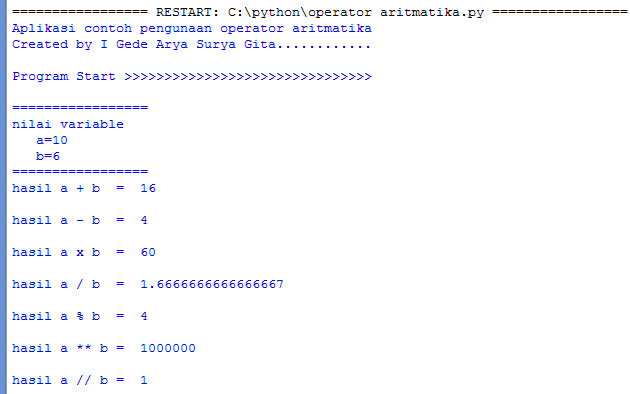
\includegraphics[width=0.25\textwidth]{figures/ctharitmatika}}
 	\caption{Contoh Operator Aritmatika}
 	\label{contoh}
\end{figure}

\vspace{12pt}
\noindent 
Bahasa Python mendukung jenis operator berikut. \par
\vspace{12pt}
\noindent 
\begin{enumerate}
	\item Operator Aritmatika 
	\item Operator Perbandingan (Relasional) 
	\item Operator Penugasan \par
	\item Operator Logis \par
	\item Bitwise Operator \par
	\item Operator keanggotaan \par
	\item Operator Identitas \par
\end{enumerate}


Mari kita lihat semua operator satu per satu. \par
\vspace{12pt}
\noindent 
Operator Aritmatika Python \par
\vspace{12pt}
\noindent 
Asumsikan variabel a memegang 10 dan variabel b memegang 20, maka  \par
\vspace{12pt}
\noindent 
+ Tambahan \par
\noindent 
Menambahkan nilai di kedua sisi operator. \par
\noindent 
Contoh A + b = 30 \par
\vspace{12pt}
\noindent 
- Pengurangan \par
\noindent 
Kurangi operan tangan kanan dari operan tangan kiri. \par
\noindent 
Contoh a - b = -10 \par
\vspace{12pt}
\noindent 
* Perkalian \par
\noindent 
Kalikan nilai di kedua sisi operator \par
\noindent 
Contoh a * b = 200 \par
\vspace{12pt}
\noindent 
/ Divisi \par
\noindent 
Membagi operan tangan kiri dengan tangan kanan operan \par
\noindent 
Contoh B / a = 2 \par
\vspace{12pt}
\noindent 
 $  \%  $ Modulus \par
\noindent 
Membagi operan tangan kiri dengan operan tangan kanan dan mengembalikan sisa \par
\noindent 
Contoh B $  \%  $ a = 0 \par
\vspace{12pt}
\noindent 
** Eksponen \par
\noindent 
Melakukan perhitungan eksponensial (daya) pada operator \par
\noindent 
Contoh A ** b = 10 ke daya 20 \par
\vspace{12pt}
\noindent 
// \par
\vspace{12pt}
\noindent 
Divisi Lantai - Pembagian operan dimana hasilnya adalah hasil bagi di mana angka setelah titik desimal dikeluarkan. $  $Tapi jika salah satu operan negatif, hasilnya berlantai, yaitu terbulatkan dari nol (menuju negatif tak terbatas): \par
\vspace{12pt}
\noindent 
9 // 2 = 4 dan 9.0 // 2.0 = 4.0, -11 // 3 = -4, -11.0 // 3 = -4.0 \par
\vspace{12pt}
\noindent 
Operator Perbandingan Python \par
\vspace{12pt}
\noindent 
Operator ini membandingkan nilai di kedua sisi dan memutuskan hubungan di antara keduanya. $  $Mereka juga disebut operator relasional. \par
\vspace{12pt}
\noindent 
Asumsikan variabel a memegang 10 dan variabel b memegang 20, maka  \par
\vspace{12pt}
\noindent 
== \par
\noindent 
Jika nilai dua operan sama, maka kondisinya menjadi benar. \par
\noindent 
Contoh (a == b) tidak benar \par
\vspace{12pt}
\noindent 
! = \par
\noindent 
Jika nilai dua operan tidak sama, maka kondisinya menjadi benar. \par
\vspace{12pt}
\noindent 
> \par
\noindent 
Jika nilai operan kiri lebih besar dari nilai operan kanan, maka kondisinya menjadi benar. \par
\noindent 
Contoh (a> b) tidak benar \par
\vspace{12pt}
\noindent 
< \par
\noindent 
Jika nilai operan kiri kurang dari nilai operan kanan, maka kondisinya menjadi benar. \par
\noindent 
Contoh (A <b) adalah benar. \par
\vspace{12pt}
\noindent 
> = \par
\noindent 
Jika nilai operan kiri lebih besar dari atau sama dengan nilai operan kanan, maka kondisinya menjadi benar. \par
\noindent 
Contoh (a> = b) tidak benar \par
\vspace{12pt}
\noindent 
<= \par
\noindent 
Jika nilai operan kiri kurang dari atau sama dengan nilai operan kanan, maka kondisinya menjadi benar. \par
\noindent 
Contoh (a <= b) adalah benar. \par
\vspace{12pt}
\noindent 
Operator Penugasan Python \par
\vspace{12pt}
\noindent 
Asumsikan variabel a memegang 10 dan variabel b memegang 20, maka - \par
\vspace{12pt}
\noindent 
= \par
\noindent 
Menetapkan nilai dari operan sisi kanan ke operan sisi kiri \hspace*{4.41in}  \par
\noindent 
Contoh : c = a + b memberi nilai a + b ke c \par
\noindent 
\vspace{12pt}
\noindent 
+ = Tambahkan DAN \par
\noindent 
Ini menambahkan operan kanan ke operan kiri dan menetapkan hasilnya ke operan kiri \par
\noindent 
Contoh : c + = a setara dengan c = c + a \par
\noindent 
\vspace{12pt}
\noindent 
- = Kurangi DAN \par
\noindent 
Ini mengurangi opera kanan dari operan kiri dan menetapkan hasilnya ke operan kiri \par
\noindent 
Contoh : c - = a setara dengan c = c – a \par
\noindent 
\vspace{12pt}
\noindent 
* = Multiply DAN \par
\noindent 
Ini mengalikan operand kanan dengan operan kiri dan menetapkan hasilnya ke operan kiri \par
\noindent 
Contoh : c * = a setara dengan c = c * a \par
\noindent 
\vspace{12pt}
\noindent 
/ = Bagilah dan \par
\noindent 
Ini membagi operan kiri dengan operan kanan dan menetapkan hasilnya ke operan kiri \par
\noindent 
Contoh : C / = a adalah setara dengan c = c / ac / = a adalah setara dengan c = c / a \par
\noindent 
\vspace{12pt}
\noindent 
 $  \%  $ = Modulus DAN \par
\noindent 
Dibutuhkan modulus menggunakan dua operan dan menetapkan hasilnya ke operan kiri \par
\noindent 
Contoh : C $  \%  $ = a setara dengan c = c $  \%  $ a \par
\noindent 
\vspace{12pt}
\noindent 
** = Eksponen DAN \par
\noindent 
Melakukan perhitungan eksponensial (daya) pada operator dan memberikan nilai pada operan kiri \par
\noindent 
Contoh : C ** = a setara dengan c = c ** a \par
\noindent 
\vspace{12pt}
\noindent 
// Divisi Lantai \par
\noindent 
Ini melakukan pembagian lantai pada operator dan memberikan nilai ke operan kiri \par
\noindent 
Contoh : C // = a sama dengan c = c // a \par
\noindent 
\vspace{12pt}
\noindent 
Operator Bitwise Python \par
\vspace{12pt}
\noindent 
Operator Bitwise bekerja pada bit dan melakukan operasi bit by bit. $  $Asumsikan jika a = 60; $  $Dan b = 13; $  $Sekarang dalam format biner mereka akan menjadi seperti berikut - \par

\begin{verbatim}
a = 0011 1100
b = 0000 1101
a & b = 0000 1100
A | b = 0011 1101
a ^ b = 0011 0001
~ a = 1100 0011
\end{verbatim}

Ada beberapa operator Bitwise berikut yang didukung oleh bahasa Python \par
\vspace{12pt}
\noindent 
 $  \&  $ Biner DAN \par
\noindent 
Operator menyalin sedikit ke hasil jika ada di kedua operan \par
\noindent 
Contoh : (A  $  \&  $ b) (berarti 0000 1100) \par
\vspace{12pt}
\noindent 
 $  \vert  $ $  $Biner ATAU \par
\noindent 
Ini salinan sedikit jika ada di salah satu operan. \par
\noindent 
Contoh : (A  $  \vert  $ b) = 61 (berarti 0011 1101) \par
\vspace{12pt}
\noindent 
 $  \string^  $ Biner XOR \par
\noindent 
Ini salinan bit jika diatur dalam satu operand tapi tidak keduanya. \par
\noindent 
Contoh : (A  $  \string^  $ b) = 49 (berarti 0011 0001) \par
\vspace{12pt}
\noindent 
 $  \sim  $ Binary Ones Complement \par
\noindent 
Ini tidak mencolok dan memiliki efek bit 'flipping'. \par
\noindent 
Contoh : ( $  \sim  $ A) = -61 (berarti bentuk pelengkap 1100 0011 dalam 2 karena nomor biner yang ditandatangani \par
\vspace{12pt}
\noindent 
<< Pergeseran Kiri Biner \par
\noindent 
Nilai operan kiri dipindahkan ke kiri oleh jumlah bit yang ditentukan oleh operan kanan. \par
\noindent 
Contoh : Sebuah << = 240 (berarti 1111 0000) \par
\vspace{12pt}
\noindent 
>> Binary Right Shift \par
\noindent 
Nilai operan kiri dipindahkan tepat dengan jumlah bit yang ditentukan oleh operan kanan. \par
\noindent 
Contoh : a >> = 15 (berarti 0000 1111) \par
\vspace{12pt}
\noindent 
Operator Logika Python \par
\vspace{12pt}
\noindent 
Ada beberapa operator logis berikut yang didukung oleh bahasa Python. $  $Asumsikan variabel a memegang 10 dan variabel b memegang 20 kemudian \par
\vspace{12pt}
\noindent 
Digunakan untuk membalik keadaan logis operannya. \par
\vspace{12pt}
\noindent 
Keanggotaan Python Operator \par
\vspace{12pt}
\noindent 
Operator keanggotaan Python menguji keanggotaan secara berurutan, seperti senar, daftar, atau tupel. $  $Ada dua operator keanggotaan seperti yang dijelaskan di bawah ini \par
\vspace{12pt}
\noindent 
Di \par
\noindent 
Mengevaluasi ke true jika menemukan sebuah variabel dalam urutan yang ditentukan dan false sebaliknya. \par
\noindent 
Contoh : X di y, di sini menghasilkan 1 jika x adalah anggota dari urutan y. \par
\vspace{12pt}
\noindent 
tidak masuk \par
\noindent 
Mengevaluasi ke true jika tidak menemukan variabel dalam urutan yang ditentukan dan false sebaliknya. \par
\noindent 
Contoh : X tidak di y, di sini tidak menghasilkan 1 jika x bukan anggota urutan y. \par
\vspace{12pt}
\noindent 
Operator Identitas Python \par
\vspace{12pt}
\noindent 
Operator identitas membandingkan lokasi memori dari dua objek. $  $Ada dua operator Identitas yang dijelaskan di bawah ini: \par
\vspace{12pt}
\noindent 
aku s \par
\noindent 
Mengevaluasi ke true jika variabel di kedua sisi operator menunjuk ke objek yang sama dan salah sebaliknya. \par
\noindent 
Contoh: X adalah y, di sini $  $adalah $  $hasil dalam 1 jika id (x) sama dengan id (y). \par
\vspace{12pt}
\noindent 
Tidak \par
\noindent 
Mengevaluasi false jika variabel di kedua sisi operator menunjuk ke objek yang sama dan benar sebaliknya. \par
\noindent 
Contoh: X bukan y, $  $ini bukan $  $hasil 1 jika id (x) tidak sama dengan id (y). \par
\vspace{12pt}
\noindent 
Operator Python Diutamakan \par
\vspace{12pt}
\noindent 
 berikut mencantumkan semua operator dari preseden tertinggi sampai yang terendah. \par
\vspace{12pt}
\noindent 
** \par
\noindent 
Eksponensiasi (naik ke tampuk kekuasaan) \par
\vspace{12pt}
\noindent 
 $  \sim  $ + - \par
\noindent 
Pelengkap, unary plus dan minus (nama metode untuk dua yang terakhir adalah + @ dan - @) \par
\vspace{12pt}
\noindent 
* / $  \%  $ // \par
\noindent 
Kalikan, bagi, modulo dan pembagian lantai \par
\vspace{12pt}
\noindent 
+ - \par
\noindent 
Penambahan dan pengurangan \par
\vspace{12pt}
\noindent 
>> << \par
\noindent 
Pergeseran bitwise kanan dan kiri \par
\vspace{12pt}
\noindent 
 $  \&  $ \par
\noindent 
Bitwise 'DAN' \par
\vspace{12pt}
\noindent 
 $  \string^  $  $  \vert  $ \par
\noindent 
Bitwise eksklusif `OR 'dan reguler` OR' \par
\vspace{12pt}
\noindent 
<= <>> = \par
\noindent 
Operator perbandingan \par
\vspace{12pt}
\noindent 
<> ==! = \par
\noindent 
Operator kesetaraan \par
\vspace{12pt}
\noindent 
= $  \%  $ = / = // = - = + = * = ** = \par
\noindent 
Operator penugasan \par
\vspace{12pt}
\noindent 
Bukan \par
\noindent 
Operator identitas \par
\vspace{12pt}
\noindent 
Bukan di \par
\noindent 
Operator keanggotaan \par
\vspace{12pt}
\noindent 
Tidak atau dan \par
\noindent 
Operator logika \par
\vspace{12pt}
\noindent 
Peran operator dalam proses perhitungan matematika sangatlah penting. Selain $  $operator Aritmatika, Python juga mendukung $  $operator berkondisi $  $yang berfungsi untuk membandingkan suatu nilai dengan nilai yang lain. Operator-operator yang didukung oleh Python yaitu $  $operator Unari $  $( + dan – ) dan $  $operator Binari $  $( +, -, *, /,  $  \%  $, dan **). Pada ekspresi Aritmatika berikut:\vspace{\baselineskip}
\vspace{\baselineskip}
x = y + z \par
\noindent 
y $  $dan $  $z $  $disebut sebagai operan dari operator $  $+. Tabel di bawah ini menjelaskan tentang berbagai macam operator yang digunakan untuk segala perhitungan di Python. \par
\vspace{12pt}
\noindent 
Jika sebuah ekspresi melibatkan lebih dari satu operator, Python secara otomatis akan memilih operator mana yang akan diutamakan dahulu. Sebagai contoh: \par
\begin{verbatim}
>>> x=7+3*6
>>> x
25
>>> y=100/4*5
>>> y
125

\end{verbatim}
Operator $  $** $  $memiliki urutan tertinggi diantara operator lainnya. Operator $  $* $  $mempunyai urutan lebih tinggi daripada operator $  $+, dan operator $  $/ $  $mempunyai urutan yang sama dengan operator $  $*. Pada ekspresi $  $x = 7 + 3 * 6, bagian $  $3 * 6 $  $akan dieksekusi pertama kali menghasilkan $  $18, yang kemudian ditambahkan dengan $  $7. Sedangkan ekspresi $  $y = 100/4*5, bagian $  $100/4dieksekusi terlebih dahulu karena operator $  $/ $  $berada disebelah kiri dari operator $  $*. \par
\vspace{12pt}
\noindent 
Kita dapat mengubah urutan prioritas dari operator Aritmatika dengan menggunakan kurung-buka-kurung-tutup $  $(). Operator $  $() $  $memiliki urutan tertinggi diantara tiga tipe lainnya. Operator $  $() $  $mempunyai urutan dari kiri ke kanan pada ekspresi di dalamnya. Berikut ini contohnya: \par
\vspace{12pt}
\noindent 
>>> x=(7+3)*6\vspace{\baselineskip}
>>> x\vspace{\baselineskip}
60\vspace{\baselineskip}
>>> y=100/(4*5)\vspace{\baselineskip}
>>> y\vspace{\baselineskip}
5\vspace{\baselineskip}
>>> z=7+(5*(8/2)+(4+6))\vspace{\baselineskip}
>>> z\vspace{\baselineskip}
37 \par
\vspace{12pt}
\noindent 
Operator modulus $  $ $  \%  $ $  $akan memberikan nilai sisa dari pembagian integer. Berikut contoh penggunaan operator modulus: \par
\vspace{12pt}
\noindent 
>>> 7  $  \%  $ 3\vspace{\baselineskip}
1\vspace{\baselineskip}
>>> 0  $  \%  $ 3\vspace{\baselineskip}
0\vspace{\baselineskip}
>>> 1.0  $  \%  $ 3.0\vspace{\baselineskip}
1.0 \par
\vspace{12pt}
\noindent 
Operator eksponensial $  $akan memberikan nilai pangkat dari suatu bilangan. Contoh penggunaan operator eksponensial: \par
\vspace{12pt}
\noindent 
>>> 5**2\vspace{\baselineskip}
25\vspace{\baselineskip}
>>> 5**-2\vspace{\baselineskip}
0.04\vspace{\baselineskip}
>>> -5**2\vspace{\baselineskip}
-25\vspace{\baselineskip}
>>> (-5)**2\vspace{\baselineskip}
25 \par
\vspace{12pt}
\noindent 
Operator Penugasan Python \par
\vspace{12pt}
\noindent 
Asumsikan variabel a memegang 10 dan variabel b memegang 20, maka - \par
\vspace{12pt}
\noindent 
= \par
\noindent 
Menetapkan nilai dari operan sisi kanan ke operan sisi kiri \hspace*{4.41in}  \par
\noindent 
Contoh : c = a + b memberi nilai a + b ke c \par
\noindent 
\vspace{12pt}
\noindent 
+ = Tambahkan DAN \par
\noindent 
Ini menambahkan operan kanan ke operan kiri dan menetapkan hasilnya ke operan kiri \par
\noindent 
Contoh : c + = a setara dengan c = c + a \par
\noindent 
\vspace{12pt}
\noindent 
- = Kurangi DAN \par
\noindent 
Ini mengurangi opera kanan dari operan kiri dan menetapkan hasilnya ke operan kiri \par
\noindent 
Contoh : c - = a setara dengan c = c – a \par
\noindent 
\vspace{12pt}
\noindent 
* = Multiply DAN \par
\noindent 
Ini mengalikan operand kanan dengan operan kiri dan menetapkan hasilnya ke operan kiri \par
\noindent 
Contoh : c * = a setara dengan c = c * a \par
\noindent 
\vspace{12pt}
\noindent 
/ = Bagilah dan \par
\noindent 
Ini membagi operan kiri dengan operan kanan dan menetapkan hasilnya ke operan kiri \par
\noindent 
Contoh : C / = a adalah setara dengan c = c / ac / = a adalah setara dengan c = c / a \par
\noindent 
\vspace{12pt}
\noindent 
 $  \%  $ = Modulus DAN \par
\noindent 
Dibutuhkan modulus menggunakan dua operan dan menetapkan hasilnya ke operan kiri \par
\noindent 
Contoh : C $  \%  $ = a setara dengan c = c $  \%  $ a \par
\noindent 
\vspace{12pt}
\noindent 
** = Eksponen DAN \par
\noindent 
Melakukan perhitungan eksponensial (daya) pada operator dan memberikan nilai pada operan kiri \par
\noindent 
Contoh : C ** = a setara dengan c = c ** a \par
\noindent 
\vspace{12pt}
\noindent 
// Divisi Lantai \par
\noindent 
Ini melakukan pembagian lantai pada operator dan memberikan nilai ke operan kiri \par
\noindent 
Contoh : C // = a sama dengan c = c // a \par
\noindent 
\vspace{12pt}
\noindent 
Operator Bitwise Python \par
\vspace{12pt}
\noindent 
Operator Bitwise bekerja pada bit dan melakukan operasi bit by bit. $  $Asumsikan jika a = 60; $  $Dan b = 13; $  $Sekarang dalam format biner mereka akan menjadi seperti berikut - \par
\vspace{12pt}
\noindent 
a = 0011 1100 \par
\vspace{12pt}
\noindent 
b = 0000 1101 \par
\vspace{12pt}
\vspace{12pt}
\noindent 
a  $  \&  $ b = 0000 1100 \par
\vspace{12pt}
\noindent 
A  $  \vert  $ b = 0011 1101 \par
\vspace{12pt}
\noindent 
a  $  \string^  $ b = 0011 0001 \par
\vspace{12pt}
\noindent 
 $  \sim  $ a = 1100 0011 \par
\vspace{12pt}
\noindent 
Ada beberapa operator Bitwise berikut yang didukung oleh bahasa Python \par
\vspace{12pt}
\noindent 
 $  \&  $ Biner DAN \par
\noindent 
Operator menyalin sedikit ke hasil jika ada di kedua operan \par
\noindent 
Contoh : (A  $  \&  $ b) (berarti 0000 1100) \par
\vspace{12pt}
\noindent 
 $  \vert  $ $  $Biner ATAU \par
\noindent 
Ini salinan sedikit jika ada di salah satu operan. \par
\noindent 
Contoh : (A  $  \vert  $ b) = 61 (berarti 0011 1101) \par
\vspace{12pt}
\noindent 
 $  \string^  $ Biner XOR \par
\noindent 
Ini salinan bit jika diatur dalam satu operand tapi tidak keduanya. \par
\noindent 
Contoh : (A  $  \string^  $ b) = 49 (berarti 0011 0001) \par
\vspace{12pt}
\noindent 
 $  \sim  $ Binary Ones Complement \par
\noindent 
Ini tidak mencolok dan memiliki efek bit 'flipping'. \par
\noindent 
Contoh : ( $  \sim  $ A) = -61 (berarti bentuk pelengkap 1100 0011 dalam 2 karena nomor biner yang ditandatangani \par
\vspace{12pt}
\noindent 
<< Pergeseran Kiri Biner \par
\noindent 
Nilai operan kiri dipindahkan ke kiri oleh jumlah bit yang ditentukan oleh operan kanan. \par
\noindent 
Contoh : Sebuah << = 240 (berarti 1111 0000) \par
\vspace{12pt}
\noindent 
>> Binary Right Shift \par
\noindent 
Nilai operan kiri dipindahkan tepat dengan jumlah bit yang ditentukan oleh operan kanan. \par
\noindent 
Contoh : a >> = 15 (berarti 0000 1111) \par
\vspace{12pt}
\noindent 
Operator Perbandingan Python \par
\vspace{12pt}
\noindent 
Operator ini membandingkan nilai di kedua sisi dan memutuskan hubungan di antara keduanya. $  $Mereka juga disebut operator relasional. \par
\vspace{12pt}
\noindent 
Asumsikan variabel a memegang 10 dan variabel b memegang 20, maka  \par
\vspace{12pt}
\noindent 
== \par
\noindent 
Jika nilai dua operan sama, maka kondisinya menjadi benar. \par
\noindent 
Contoh (a == b) tidak benar \par
\vspace{12pt}
\noindent 
! = \par
\noindent 
Jika nilai dua operan tidak sama, maka kondisinya menjadi benar. \par
\vspace{12pt}
\noindent 
> \par
\noindent 
Jika nilai operan kiri lebih besar dari nilai operan kanan, maka kondisinya menjadi benar. \par
\noindent 
Contoh (a> b) tidak benar \par
\vspace{12pt}
\noindent 
< \par
\noindent 
Jika nilai operan kiri kurang dari nilai operan kanan, maka kondisinya menjadi benar. \par
\noindent 
Contoh (A <b) adalah benar. \par
\vspace{12pt}
\noindent 
> = \par
\noindent 
Jika nilai operan kiri lebih besar dari atau sama dengan nilai operan kanan, maka kondisinya menjadi benar. \par
\noindent 
Contoh (a> = b) tidak benar \par
\vspace{12pt}
\noindent 
<= \par
\noindent 
Jika nilai operan kiri kurang dari atau sama dengan nilai operan kanan, maka kondisinya menjadi benar. \par
\noindent 
Contoh (a <= b) adalah benar. \par
\noindent 
Operator Python Diutamakan \par
\vspace{12pt}
\noindent 
 berikut mencantumkan semua operator dari preseden tertinggi sampai yang terendah. \par
\vspace{12pt}
\noindent 
** \par
\noindent 
Eksponensiasi (naik ke tampuk kekuasaan) \par
\vspace{12pt}
\noindent 
 $  \sim  $ + - \par
\noindent 
Pelengkap, unary plus dan minus (nama metode untuk dua yang terakhir adalah + @ dan - @) \par
\vspace{12pt}
\noindent 
* / $  \%  $ // \par
\noindent 
Kalikan, bagi, modulo dan pembagian lantai \par
\vspace{12pt}
\noindent 
+ - \par
\noindent 
Penambahan dan pengurangan \par
\vspace{12pt}
\noindent 
>> << \par
\noindent 
Pergeseran bitwise kanan dan kiri \par
\vspace{12pt}
\noindent 
 $  \&  $ \par
\noindent 
Bitwise 'DAN' \par
\vspace{12pt}
\noindent 
 $  \string^  $  $  \vert  $ \par
\noindent 
Bitwise eksklusif `OR 'dan reguler` OR' \par
\vspace{12pt}
\noindent 
<= <>> = \par
\noindent 
Operator perbandingan \par
\vspace{12pt}
\noindent 
<> ==! = \par
\noindent 
Operator kesetaraan \par
\vspace{12pt}
\noindent 
= $  \%  $ = / = // = - = + = * = ** = \par
\noindent 
Operator penugasan \par
\vspace{12pt}
\noindent 
Bukan \par
\noindent 
Operator identitas \par
\vspace{12pt}
\noindent 
Bukan di \par
\noindent 
Operator keanggotaan \par
\vspace{12pt}
\noindent 
Tidak atau dan \par
\noindent 
Operator logika \par
\vspace{12pt}
\vspace{12pt}



\chapter{Desicion Making}
\section{Python Decision Making}
Pengambilan keputusan adalah antisipasi kondisi yang terjadi saat pelaksanaan program dan menentukan tindakan yang dilakukan sesuai kondisi. 
Struktur keputusan mengevaluasi banyak ekspresi yang menghasilkan TRUE atau FALSE sebagai hasil. \$  \$Anda perlu menentukan tindakan mana yang harus diambil dan pernyataan mana yang akan dijalankan jika hasilnya BENAR atau SALAH sebaliknya. 
Berikut adalah bentuk umum dari struktur pengambilan keputusan yang khas atau khusus yang ditemukan di sebagian besar bahasa pemrograman
\ref{struktur}.
\begin{figure}[ht]
    \centerline{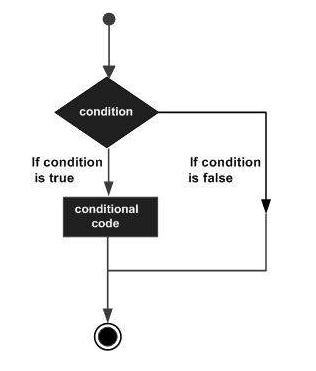
\includegraphics[width=0.25\textwidth]{figures/struktur.png}}
    \caption{struktur pada python}
    \label{struktur}
    \end{figure}\par
Bahasa pemrograman Python menyediakan jenis dan juga laporan pengambilan keputusan. Berikut ini adalah penjelasan tentang pernyataan dan deskripsinya :
\begin{enumerate}
\item
if statements : sebuah if statement terdiri dari ekspresi boolean diikuti oleh satu atau lebih pernyataan. \par
\item
if...else statements : sebuah if statement dapat diikuti oleh opsinal else statement, yang mengeksekusi ketika ekspresi boolean adalah palsu. \par
\item
nested if statements : anda dapat menggunakan satu if atau else if pernyataan di dalam lain if atau else if statements. \par
\end{enumerate}
Decision making atau Pemilihan keputusan pada python sangat penting untuk pemrograman komputer. Akan ada banyak situasi saat Anda diberi dua pilihan atau lebih dan Anda harus memilih opsi berdasarkan kondisi yang diberikan. Misalnya,
\begin{enumerate} \par
\item
Seorang murid dengan nilai lebih dari 90 disebut siswa pintar \par
\item
Seorang murid dengan nilai dibawah 90 dan diatas 30 disebut Siswa Standard \par
\item
Seorang murid dengan nilai dibawah 30 disebut siswa bodoh \par
\end{enumerate}\par

Umumnya juga, decision making dalam bahasa pemrograman yang sering digunakan adalah :
\begin{enumerate}
\item
if...else statement : berguna saat kita harus mengambil keputusan dari dua pilihan. Misalnya, jika seorang siswa mendapatkan nilai lebih dari angka 95, maka siswa itu pintar, jika tidak, situasi seperti itu dapat dikodekan. \par
\item
if...elseif...else statement : merupakan optional dari if...else statement, yang sangat berguna untuk menentukan berbagai kondisi yang lebih dari 2. \par
\item
switch statement : merupakan alternative dari if statement. Setiap nilai disebut case, dan variabel yang dicek untuk setiap switch case. \par
\end{enumerate}

Dari contoh diatas, pertanyaannya adalah bagaimana cara menulis kode pemrograman untuk menangani situasi seperti itu. Hampir semua bahasa pemrograman memberikan pernyataan kondisional diatas berdasarkan diagram decision di bawah. \par
\begin{figure}[ht]
	    \centerline{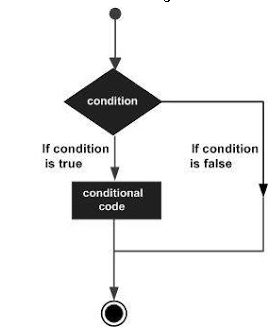
\includegraphics[width=0.25\textwidth]{figures/diagram_decision.png}}
	    \caption{diagram decision}
	    \label{diagram_decision}
	    \end{figure} \par

Mari kita membuat sebuah program C dengan bantuan jika pernyataan kondisional untuk mengubah situasi yang diberikan di atas menjadi kode pemrograman: \par 
\begin{verbatim}
#include <stdio.h>
 
main() {
   int x = 45;
   if( x > 95) {
      printf( "siswa pintar");
   }
   if( x < 30) {
      printf( "siswa bodoh");
   }
   if( x < 95 && x > 30 ) {
      printf( "Siswa Standard");
   }
}
\end{verbatim}\par
Outputnya adalah Siswa Standard

Bahasa pemrograman Python mengasumsikan nilai \$  \$non-nol \$  \$dan \$  \$non-nullsebagai TRUE, dan jika itu adalah \$  \$nol \$  \$atau \$  \$nol \$  \$, maka diasumsikan sebagai nilai FALSE. \par
Bahasa pemrograman Python menyediakan jenis pernyataan pengambilan keputusan berikut. \par
\vspace{12pt}
\noindent 
Mari kita membahas setiap keputusan secara singkat  \par
\vspace{12pt}
\noindent 
Setelah tutorial mengenai \$ 
\subsection{variable dan operator}
\$pada bahasa pemrograman python akan membahas mengenai percabangan/pengambilan keputusan. Percabangan atau pengambilan keputusan adalah pengkondisian yang terjadi ketika aplikasi berjalan, kemudian ada aksi-aksi tertentu atau kondisi tertentu sehingga aplikasi harus bereaksi terhadap hal itu. Atau dalam bahasa pemrograman umum dikenal dengan IF, THEN, ELSE sebagai contoh pengaplikasian dari pengambilan keputusan ini. \par
\vspace{12pt}
if statements
Sebuah if statement terdiri dari ekspresi boolean diikuti oleh satu atau lebih pernyataan.
\noindent 
Pada pembahasan python decisiom makaing ini, kami menggunakan perangkat raspberry pi 2 dengan sistem operasi rasbian jessie. Sangat ringan dan tentunya python secara default ada di dalamnya. Kebetulan dalam tulisan ini masih menggunakan python versi 2, meskipun ada python versi 3 juga. \par
\vspace{12pt}
\noindent 
Python core tidak menyediakan  \$ \" \$switch \$ \" \$ atau  \$ " \$case \$ \" \$ seperti bahasa pemrograman lain. Tapi kita bisa menggunakan statemen if, elif yang bisa menggantikan  \$ \" \$switch \$ \" \$ atau  \$ \" \$case \$ \" \$. \par
\vspace{12pt}
\noindent 
Di bawah ini merupakan tipe-tipe percabangan yang disediakan oleh python. \par
\vspace{12pt}
\noindent 
IF : Mengandung ekspresi boolean dan diikuti oleh satu atau banyak statemen \par
\vspace{12pt}
\noindent 
IF ELSE : IF bisa diikuti oleh optional statemen yaitu ELSE, yang akan dieksekusi ketika ekspresi boolean bernilai FALSE \par
\vspace{12pt}
\noindent 
NESTED IF atau IF bersarang :~ Kita bisa menggunakan IF, ELSE IF di dalam IF, ELSE IF lainnya \par
\vspace{12pt}
\noindent 
Contoh dalam python untuk IF :  \par
\vspace{12pt}
\noindent 
varAngka1 = 123 \par
\vspace{12pt}
\noindent 
varAngka2 = 0 \par
\vspace{12pt}
\noindent 
if varAngka1: \par
\vspace{12pt}
\noindent 
 \$  \$ \$  \$ \$  \$ \$  \$ \$ \$ \$  \$ \$  \$ \$  \$ \$  \$ \$  \$ \$  \$ \$  \$ \$  \$ \$  \$ \$  \$ \$  \$print "Nilai : TRUE" \par
\vspace{12pt}
\noindent 
 \$  \$ \$  \$ \$  \$ \$  \$ \$  \$ \$  \$ \$  \$ \$  \$ \$  \$ \$  \$ \$  \$ \$  \$ \$  \$ \$  \$ \$  \$ \$  \$print varAngka1 \par
\vspace{12pt}
\noindent 
if varAngka2: \par
\vspace{12pt}
\noindent 
 \$  \$ \$  \$ \$  \$ \$  \$ \$ \$ \$  \$ \$  \$ \$  \$ \$  \$ \$  \$ \$  \$ \$  \$ \$  \$ \$  \$ \$  \$ \$  \$print "Nilai : TRUE" \par
\vspace{12pt}
\noindent 
 \$  \$ \$  \$ \$  \$ \$  \$ \$ \$ \$  \$ \$  \$ \$  \$ \$  \$ \$  \$ \$  \$ \$  \$ \$  \$ \$  \$ \$  \$ \$  \$print varAngka2{\fontsize{14pt}{14pt}\selectfont  \$  \$ \\} \par
\vspace{12pt}
\noindent 
Begin{verbatim}
#/usr/bin/python
a = raw_input("Masukkan Angka = ")
b = int(a)
if (b%2==0):
        print "Genap"
else:
        print "Ganjil"
end{verbatim}

Contoh untuk IF ELIF ELSE, di python sintak ini bisa ditulis dengan lebih singkat yaitu elif :  \par
\vspace{12pt}
\noindent 
varAngka = 123 \par
\noindent 
 \$  \$ \par
\noindent 
if varAngka==200: \par
\vspace{12pt}
\noindent 
 \$  \$  \$  \$  \$  \$  \$  \$  \$  \$  \$  \$  \$  \$print "Nilai : TRUE" \par
\vspace{12pt}
\noindent 
 \$  \$  \$  \$  \$  \$  \$  \$  \$  \$  \$  \$  \$  \$print varAngka \par
\vspace{12pt}
\noindent 
elif varAngka==123: \par
\vspace{12pt}
\noindent 
 \$  \$  \$  \$  \$  \$  \$  \$  \$  \$  \$  \$  \$  \$print "Nilai : TRUE" \par
\vspace{12pt}
\noindent 
 \$  \$  \$  \$  \$  \$  \$  \$  \$  \$  \$  \$  \$  \$print varAngka \par
\vspace{12pt}
\noindent 
else: \par
\vspace{12pt}
\noindent 
 \$  \$  \$  \$  \$  \$  \$  \$  \$  \$  \$  \$  \$  \$print "Nilai : FALSE" \par
\vspace{12pt}
\noindent 
 \$  \$  \$  \$  \$  \$  \$  \$  \$  \$  \$  \$  \$  \$print varAngka \par
\vspace{12pt}
\noindent 
Contoh untuk NESTED IF :  \par
\vspace{12pt}
\begin{verbatim}
varAngka = 89 \par
\noindent 
 \$  \$ \par
\noindent 
if varAngka<100: \par
\vspace{12pt}
\noindent 
 \$  \$  \$  \$  \$  \$  \$  \$  \$  \$  \$  \$print \"Nilai : TRUE\" \par
\vspace{12pt}
\noindent 
 \$  \$  \$  \$  \$  \$  \$  \$  \$  \$  \$  \$print varAngka \par
\vspace{12pt}
\noindent 
 \$  \$  \$  \$  \$  \$  \$  \$  \$  \$  \$  \$if varAngka > 80: \par
\vspace{12pt}
\noindent 
 \$  \$  \$  \$  \$  \$  \$  \$  \$  \$  \$  \$  \$  \$  \$  \$  \$  \$  \$  \$  \$  \$  \$  \$ print \"Nilai : A\" \par
\vspace{12pt}
\noindent 
 \$  \$  \$  \$  \$  \$  \$  \$  \$  \$  \$  \$elif varAngka > 60: \par
\vspace{12pt}
\noindent 
 \$  \$  \$  \$  \$  \$  \$  \$  \$  \$  \$  \$  \$  \$  \$  \$  \$  \$  \$  \$  \$  \$  \$  \$ print \"Nilai : B\" \par
\vspace{12pt}
\noindent 
\$  \$  \$  \$  \$  \$  \$  \$  \$  \$  \$   \$elif varAngka > 40: \par
\vspace{12pt}
\noindent 
 \$  \$  \$  \$  \$  \$  \$  \$  \$  \$  \$  \$  \$  \$  \$  \$  \$  \$  \$  \$  \$  \$  \$ print \"Nilai : C\" \par
\vspace{12pt}
\noindent 
 \$  \$  \$  \$  \$  \$  \$  \$  \$  \$  \$  \$elif varAngka > 20: \par
\vspace{12pt}
\noindent 
\$  \$  \$  \$  \$  \$  \$  \$  \$  \$  \$  \$  \$  \$  \$  \$  \$  \$  \$  \$  \$  \$  \$ print \"Nilai : D\" \par
\vspace{12pt}
\noindent 
  \$  \$  \$  \$  \$  \$  \$  \$  \$  \$  \$  $else: \par
\vspace{12pt}
\noindent 
\$  \$  \$  \$  \$  \$  \$  \$  \$  \$  \$  \$  \$  \$  \$  \$  \$  \$  \$  \$  \$  \$  \ print \"Nilai : E\" \par
\vspace{12pt}
\noindent 
else: \par
\vspace{12pt}
\noindent  \$  \$  \$  \$  \$  \$  \$  \$  \$  \$  \$  \$print \"Nilai : FALSE\" \par
\vspace{12pt}
\noindent 
  \$  \$  \$  \$  \$  \$  \$  \$  \$  \$  \$  \$print varAngka \par
  end{verbatim}
\vspace{12pt}
\noindent
Contoh lain pada NESTED IF dengan kondisi pilihan lebih dari satu. Seperti menentukan game yang sangat disukai : \par
\vspace{12}
\noindent 
Begin{verbatim}
#/usr/bin/python
pilihan=2
if pilihan==1:
        print "DOTA 2"
else:
        if pilihan==2:
		print "GTA V Online"
	else:
		print "Semua Game"
end{verbatim}
\noindent
Perintah seperti diatas itu adalah NESTED IF yaitu terdapat IF di dalam IF. \par
\vspace{12pt}
\noindent 
Statemen IF juga bisa ditulis dalam 1 baris saja, misalnya seperti ini :  \par
\vspace{12pt}
\noindent 
if varAngka1: print \"Nilai : TRUE\" \par
\vspace{12pt}
\noindent 
Dari sintak percabangan sudah bisa kita lihat perbedaan di antara python dengan menggunakan bahasa pemrograman yang lain. Sintak ditulis dengan lebih ringkas dibanding dengan yang lain. Percabangan atau pengkondisian ini adalah hal dasar dalam pemrograman pada umumnya, kita pasti akan menggunakannya. Pada tulisan yang akan dibuat selanjutnya saya akan menulis mengenai perulangan atau looping dalam python. \par
\vspace{12pt}
\noindent 
Suite pernyataan tunggal \par
\vspace{12pt}
\noindent 
Jika rangkaian \$  \$klausa \$  \$jika \$  \$hanya terdiri dari satu baris, itu mungkin sama pada baris perintah sebagai pernyataan header. \par
\vspace{12pt}
\noindent 
Berikut adalah contoh \$  \$klausa \$  \$satu baris jika \$  \$- \par
\vspace{12pt}
\vspace{12pt}
\noindent 
var = 100 \par
\vspace{12pt}
\noindent 
if ( var~ == 100 ) : print "Value of expression is 100" \par
\vspace{12pt}
\noindent 
print "Good bye!" \par
\vspace{12pt}
\noindent 
Bila kode diatas dieksekusi, maka menghasilkan hasil sebagai berikut - \par
\vspace{12pt}
\noindent 
Value of expression is 100 \par
\vspace{12pt}
\noindent 
Good bye! \hspace*{1.31in}  \par
\noindent 
\vspace{12pt}
\noindent 
Pengambilan keputusan (kondisi if) digunakan untuk mengantisipasi kondisi yang terjadi saat jalanya program dan menentukan tindakan apa yang akan diambil sesuai dengan kondisi. \par
\noindent 
\vspace{12pt}
\noindent 
Pada python ada beberapa statement atau kondisi diantaranya adalah \$  \$if, \$  \$else \$  \$dan \$  \$elif \$  \$Kondisi \$  \$if \$  \$digunakan untuk mengeksekusi kode jika kondisi bernilai benar. \par
\noindent 
\vspace{12pt}
\noindent 
Jika kondisi bernilai salah maka statement atau kondisi if tidak akan di-eksekusi. \par
\noindent 
\vspace{\baselineskip}
Dibawah ini adalah contoh penggunaan kondisi if pada Python \par
\noindent 
\vspace{\baselineskip}
Dari contoh diatas, jika program dijalankan maka akan mencetak string \"Selamat Anda Lulus Ujian\" sebanyak 1 kali yaitu pada if pertama. Di if kedua statement bernilai salah, jadi perintah \$  \$print(\"Selamat Anda Lulus\") \$  \$tidak akan dieksekusi. \par
\noindent 
\vspace{\baselineskip}
Selanjutnya Anda bisa mempelajari kondisi if else \par
\vspace{12pt}
\noindent 
Pengambilan keputusan (kondisi if else) tidak hanya digunakan untuk menentukan tindakan apa yang akan diambil sesuai dengan kondisi, tetapi juga digunakan untuk menentukan tindakan apa yang akan diambil atau dijalankan jika kondisi tidak sesuai.\vspace{\baselineskip}
\vspace{\baselineskip}
 \par
\noindent 
Pada python ada beberapa statement atau kondisi diantaranya adalah \$  \$if, \$  \$else \$  \$dan \$  \$elif \$  \$Kondisi \$  \$if \$  \$digunakan untuk mengeksekusi kode jika kondisi bernilai benar.\vspace{\baselineskip}
\vspace{\baselineskip}
 \par
\noindent 
Kondisi if else adalah kondisi dimana jika pernyataan benar (true) maka kode dalam if akan dieksekusi, tetapi jika bernilai salah (false) maka akan mengeksekusi kode di dalam else.\vspace{\baselineskip}
\vspace{\baselineskip}
 \par
\noindent 
Dibawah ini adalah contoh penggunaan kondisi if else pada Python \par
\vspace{12pt}
\noindent 
Kondisi if else adalah jika kondisi bernilai TRUE maka akan dieksekusi pada if, tetapi jika bernilai FALSE maka akan dieksekusi kode pada else \par
\noindent 
\vspace{\baselineskip}
nilai = 3\vspace{\baselineskip}
 \par
\noindent 
Jika pernyataan pada if bernilai TRUE maka if akan dieksekusi, tetapi jika FALSE kode pada else yang akan dieksekusi.\vspace{\baselineskip}
 \par
\noindent 
if(nilai > 7):\vspace{\baselineskip}
 \$  \$  \$  \$ \par
\noindent 
 print(\"Selamat Anda Lulus\")\vspace{\baselineskip}
 \par
\noindent 
else:\vspace{\baselineskip}
 \par
\noindent 
 \$  \$  \$  \$ print(\"Maaf Anda Tidak Lulus\") \par
\noindent 
\vspace{\baselineskip}
\vspace{\baselineskip}
Pada contoh diatas, jika program dijalankan maka akan mencetak string \"Maaf Anda Tidak Lulus\" karena pernyataan pada if bernilai FALSE \par
\noindent 
\vspace{\baselineskip}
Selanjutnya kita akan mempelajari per-kondisi an pada python yang terakhir yaitu \"Elif\" \$  \$ \par
\vspace{12pt}
\noindent 
Pengambilan keputusan (kondisi if elif) merupakan lanjutan atau percabangan logika dari \"kondisi if\". Dengan elif kita bisa membuat kode program yang akan menyeleksi beberapa kemungkinan yang bisa terjadi. Hampir sama dengan kondisi \"else\", bedanya kondisi \"elif\" bisa banyak dan tidak hanya satu. \$  \$\vspace{\baselineskip}
\vspace{\baselineskip}
Dibawah ini adalah contoh penggunaan kondisi elif pada Python \par
\vspace{12pt}
\noindent 
Contoh penggunaan kondisi elif \par
\vspace{12pt}
\noindent 
hari \$  \_  \$ini = \"Minggu\" \par
\noindent 
\vspace{\baselineskip}
\vspace{\baselineskip}
if(hari \$  \_  \$ini == \"Senin\"): \par
\noindent 
\vspace{\baselineskip}
 \$  \$  \$  \$ print(\"Saya akan kuliah\") \par
\noindent 
\vspace{\baselineskip}
elif(hari \$  \_  \$ini == \"Selasa\"): \par
\noindent 
\vspace{\baselineskip}
 \$  \$  \$  \$ print(\"Saya akan kuliah\") \par
\noindent 
\vspace{\baselineskip}
elif(hari \$  \_  \$ini == \"Rabu\"): \par
\noindent 
\vspace{\baselineskip}
 \$  \$  \$  \$ print(\"Saya akan kuliah\") \par
\noindent 
\vspace{\baselineskip}
elif(hari \$  \_  \$ini == \"Kamis\"): \par
\noindent 
\vspace{\baselineskip}
 \$  \$  \$  \$ print(\"Saya akan kuliah\") \par
\noindent 
\vspace{\baselineskip}
elif(hari \$  \_  \$ini == \"Jumat\"): \par
\noindent 
\vspace{\baselineskip}
 $  $  $  $ print("Saya akan kuliah") \par
\noindent 
\vspace{\baselineskip}
elif(hari $  \_  $ini == "Sabtu"): \par
\noindent 
\vspace{\baselineskip}
 $  $  $  $ print("Saya akan kuliah") \par
\noindent 
\vspace{\baselineskip}
elif(hari $  \_  $ini == "Minggu"): \par
\noindent 
\vspace{\baselineskip}
 $  $  $  $ print("Saya akan libur") \par
\noindent 
\vspace{\baselineskip}
\vspace{\baselineskip}
Pada contoh diatas, jika program dijalankan maka akan mencetak \$  
\$\"Saya akan libur\". \par
\noindent 
 \$  \$ Pernyataan tersebut digunakan untuk pengambilan keputusan dalam python berupa if, pernyataan tersebut memiliki format lengkap  yang dapat dilihat sebagai berikut : \par
\vspace{12pt}
\noindent 
\begin{enumerate}
\item
if kondisi \$  \_  \$1: \par
\vspace{12pt}
\noindent 
~~~~~~ pernyataan \$  \_  \$pernyataan \$  \_  \$1 \par
\vspace{12pt}
\noindent 
\item
elif kondisi \$  \_  \$2: \par
\vspace{12pt}
\noindent 
~~~~~~ pernyataan \$  \_  \$pernyataan \$  \_  \$2 \par
\vspace{12pt}
\noindent 
\item
elif kondisi \$  \_  \$3: \par
\vspace{12pt}
\noindent 
~~~~~~ pernyataan \$  \_  \$pernyataan \$  \_  \$3 \par
\vspace{12pt}
\noindent 
\item
else kondisi \$  \_  \$n: \par
\vspace{12pt}
\noindent 
~~~~~~ pernyataan \$  \_  \$pernyataan-n \par
\vspace{12pt}
\noindent 
~~~~~~  \par
\noindent 
\item
if kondisi \$  \_  \$1,elif kondisi \$  \_  \$2,elif kondisi \$  \_  \$3,else kondisi \$  \_  \$n \par
\vspace{12pt}
\noindent 
~~~~berupa~suatu ekspresi yang menghasilkan nilai logika (benar atau salah)    \par
\noindent 
~~~  \par
\end{enumerated}
\noindent 
Contoh Code yang dijalankan pada modus interaktif \par
\vspace{12pt}
\noindent
\begin{verbatim}
  x = 5 \par
\vspace{12pt}
\noindent 
~ y = 100 \par
\vspace{12pt}
\noindent 
~~~ terbesar = x \par
\vspace{12pt}
\noindent 
~~ if terbesar < y: \par
\vspace{12pt}
\noindent 
terbesar = y \par
\vspace{12pt}
~~~ terbesar = 100  \par
\vspace{12pt}
\end{verbatim}
\noindent 
~~~  \par
\vspace{12pt}
\noindent 
 \$ \$Python tidak menggunakan \$ \{ \$ \$ \} \$ untuk menyertakan blok kode untuk penggunaan if or loop or fungsi yang lainnya. Sebaliknya, python menggunakan titik dua (:) dan indentasi atau spasi untuk pernyataan \$ \$kelompok. Tes \$ \$boolean untuk if tidak perlu dalam tanda kurung (perbedaan besar dari C++ atau Java), dan dapat memiliki *elif* dan *else*. \par
\noindent 
\vspace{\baselineskip}
 \$  \$ \$  \$ \$  \$ \$  \$Nilai apapun dapat digunakan sebagai if-test. pada  \$ \" \$nol \$ \" \$ nilai-nilai semua dihitung sebagai false:Tidak ada,0,string kosong,list kosong, dictionary kosong. Ada juga tipe Boolean dengan dua nilai: True dan False (jika dikonversi ke int, ini adalah 1 dan 0). Python memiliki operasi perbandingan yang biasa: ==, =, <, <=,>,> =. Tidak seperti Java dan C.Operator boolean bisa juga di eja seperti * and *, * or *, * not * (Python tidak menggunakan gaya C  \$  \&  \$  \$  \&  \$  \$  \vert  \$  \$  \vert  \$!). \par
\vspace{12pt}
\noindent 
~~~~matakuliah = 'matematika'   matematika,fisika \par
\noindent 
~~  \par
\noindent 
 nilai = 70 100,80,50 \par
\vspace{12pt}
\noindent 
~~~ if nilai >=100 or nilai>=80 : \par
\vspace{12pt}
\noindent 
~~~~~~ if matakuliah == 'matematika': \par
\vspace{12pt}
\noindent 
~~~~~~~~~ print 'anda mendapat nilai A dalam mata kuliah matematika' \par
\vspace{12pt}
\noindent 
~~~ elif matakuliah == 'fisika': \par
\vspace{12pt}
\noindent 
~~~~~~ print 'anda mendapat nilai A dalam mata kuliah Fisika' \par
\vspace{12pt}
\noindent 
~~~ elif nilai >=70 and matakuliah=='matematika': \par
\vspace{12pt}
\vspace{12pt}
\noindent 
~~~~~~ print 'anda mendapat nilai B dalam mata kuliah matematika' \par
\vspace{12pt}
\noindent 
~~~ elif nilai >=70 and matakuliah=='fisika': \par
\vspace{12pt}
\noindent 
~~~~~~ print 'anda mendapat nilai B dalam mata kuliah fisika' \par
\vspace{12pt}
\noindent 
~~~ else: \par
\vspace{12pt}
\noindent 
~~~~~~ print 'nilai dan~matakuliah~tidak~ada'~~~     \par
\vspace{12pt}
\noindent 
Seperti halnya bahasa pemrograman yang lain, tentu python juga mempunyai perintah untuk pengambilan suatu keputusan terhadap kondisi tertentu, yang disebut percabangan. Percabangan pada bahasa pemrograman python menggunakan perintah if, ya sama dengan bahasa pemrograman yang lain. Bagaimana cara menggunakan perintah if ini dalam bahasa pemrograman python? berikut adaah cara penggunaan percabangan if yang tepat\par
\noindent 
\vspace{\baselineskip}
Cara penulisan dari perintah if secara garis besar adalah seperti berikut: \par
\noindent 
\vspace{\baselineskip}
\vspace{\baselineskip}
if <kondisi 1>: \par
\noindent 
\vspace{\baselineskip}
 \$  \$<perintah yang dijalankan 1> \par
\noindent 
\vspace{\baselineskip}
elif <kondisi 2>: \par
\noindent 
\vspace{\baselineskip}
<perintah yang dijalankan 2> \par
\noindent 
\vspace{\baselineskip}
else:\vspace{\baselineskip}
 \$  \$<perintah yang dijalankan 3> \par
\noindent 
\vspace{\baselineskip}
\vspace{\baselineskip}
Perintah-perintah yang dipergunakan antara lain \par
\noindent 
\vspace{\baselineskip}
If dan If bersarang \par
\noindent 
\vspace{\baselineskip}
Elif (singkatan dari: else if) dan \par
\noindent 
\vspace{\baselineskip}
else.\vspace{\baselineskip}
 \par
\noindent 
\vspace{\baselineskip}
IF Bersarang \par
\noindent 
\vspace{\baselineskip}
Adapun tanda titik dua diletakan setelah kondisi, sedangkan untuk perintah yang dijalankan jika kondisi if terpenuhi diberi tab atau 4 spasi pada depannya untuk menandakan bahwa perintah tersebut berada didalam if, contoh dalam source code. Misal kita ingin menentukan angka genap atau ganjil: \par
\noindent 
\vspace{\baselineskip}
angka = 7 \par
\noindent 
\vspace{\baselineskip}
if angka  \$  \%  \$ 2 == 0: \par
\noindent 
\vspace{\baselineskip}
 \$  \$  \$  \$ print 'genap' \par
\noindent 
\vspace{\baselineskip}
else:\vspace{\baselineskip}
 \$  \$print 'ganjil' \par
\noindent 
\vspace{\baselineskip}
 Dari perintah diatas akan menghasilkan nilai yang diprint adalah 'ganjil'. Tanda  $  \%  $ (persen) disini merupakan operator untuk modulus, yaitu sisa bagi. Adapun jalannya dari program diatas adalah, jika angka dalam hal ini nilainya 7 jika di modulus dengan 2, menyisahkan nilai nol maka data yang diprint adalah genap, jika tidak menyisahkan nilai nol maka data yang diprint adalah ganjil. \par
\noindent 
\vspace{\baselineskip}
Bagaimana halnya dengan kondisi yang lebih dari satu. Misal kita ingin menentukan game yang kita sukai: \par
\noindent 
\vspace{\baselineskip}
pilihan = 2 \par
\noindent 
\vspace{\baselineskip}
if pilihan == 1: \par
\noindent 
\vspace{\baselineskip}
 \$  \$  \$  \$ print 'DOTA2' \par
\noindent 
\vspace{\baselineskip}
else:\vspace{\baselineskip}
 \$  \$  \$  \$ if pilihan == 2: \par
\noindent 
\vspace{\baselineskip}
 \$  \$  \$  \$  \$  \$  \$  \$ print 'GTA V Online' \par
\noindent 
\vspace{\baselineskip}
 \$  \$  \$  \$ else: \par
\noindent 
\vspace{\baselineskip}
 \$  \$  \$  \$  \$  \$  \$  \$ print 'Semua Game' \par
\noindent 
\vspace{\baselineskip}
Perintah diatas merupakan if bersarang yaitu terdapat if didalam if, dapat juga dituliskan dengan perintah dibawah ini dengan menggunakan elif: \par
\noindent 
\vspace{\baselineskip}
\vspace{\baselineskip}
Elif \par
\noindent 
\vspace{\baselineskip}
Merupakan suatu pemilihan kondisi dimana dalam kondisi tersebut, terdapat lagi kondisi lain\vspace{\baselineskip}
Contoh kodingnya : \par
\noindent 
\vspace{\baselineskip}
Program Kategori Berat hewan qurban \par
\noindent 
\vspace{\baselineskip}
pilihan = 300 \par
\noindent 
\vspace{\baselineskip}
if pilihan > 300: \par
\noindent 
\vspace{\baselineskip}
 \$  \$  \$  \$ print 'Sapi boleh diqurban' \par
\noindent 
\vspace{\baselineskip}
elif pilihan <  \$  \$300 : \par
\noindent 
\vspace{\baselineskip}
 \$  \$  \$  \$ print 'Sapi belum boleh diqurban' \par
\noindent 
\vspace{\baselineskip}
else: \par
\noindent 
\vspace{\baselineskip}
 \$  \$  \$  \$ print ‘Rawat dulu sapinya yang benar' \par
\noindent 
\vspace{\baselineskip}
Mana yang terbaik dari kedua cara penulisan kondisi if yang lebih dari satu diatas itu tentunya sesuai dengan kebutuhan kita masing-masing dalam membuat suatu aplikasi. Dalam if pun kita bisa membuat dua atau lebih persyaratan dalam kondisi if \par
\noindent 
\vspace{\baselineskip}
\vspace{\baselineskip}
Else \par
\noindent 
\vspace{\baselineskip}
contohnya:\vspace{\baselineskip}
angka = 2 \par
\noindent 
\vspace{\baselineskip}
if angka <= 10 and angka >= 1 : \par
\noindent 
\vspace{\baselineskip}
 \$  \$  \$  \$ print 'angka diantara 1 dan 10' \par
\noindent 
\vspace{\baselineskip}
else: \par
\noindent 
\vspace{\baselineskip}
 \$  \$  \$  \$ print 'angka diluar jangkauan' \par
\vspace{12pt}
\noindent 
Percabangan Pada Bahasa Pemrograman Python. \par
\vspace{12pt}
\noindent 
Seperti halnya bahasa pemrograman yang lain, tentu python juga mempunyai perintah untuk pengambilan suatu keputusan terhadap kondisi tertentu, yang disebut percabangan. Percabangan pada bahasa pemrograman python menggunakan perintah \$  \$if, ya sama dengan bahasa pemrograman yang lain. Bagaimana cara menggunakan perintah \$  \$if \$  \$ini dalam bahasa pemrograman python? Yuk mari kita sama-sama melihat cara penggunaan perintah \$  \$if \$  \$ini. \par
\vspace{12pt}
\noindent 
Cara penulisan dari perintah if secara garis besar adalah seperti berikut: \par
\noindent 
if <kondisi 1>: \par
\vspace{12pt}
\noindent 
~~~ <perintah yang dijalankan 1> \par
\vspace{12pt}
\noindent 
elif <kondisi 2>: \par
\vspace{12pt}
\noindent 
~~~ <perintah yang dijalankan 2> \par
\vspace{12pt}
\noindent 
else: \par
\vspace{12pt}
\noindent 
~~~ <perintah yang dijalankan 3> \par
\vspace{12pt}
\noindent 
Perintah-perintah yang dipergunakan antara lain \$  \$if, \$  \$elif \$  \$(singkatan dari: \$  \$else if) dan \$  \$else. Adapun tanda titik dua diletakan setelah kondisi, sedangkan untuk perintah yang dijalankan jika kondisi if terpenuhi diberi \$  \$tab \$  \$atau \$  \$4 spasi \$  \$pada depannya untuk menandakan bahwa perintah tersebut berada didalam if, contoh dalam source code. Misal kita ingin menentukan angka genap atau ganjil: \par
\vspace{12pt}
\noindent 
angka = 7 \par
\vspace{12pt}
\noindent 
if angka  \$  \%  \$ 2 == 0: \par
\vspace{12pt}
\noindent 
~~~ print 'genap' \par
\vspace{12pt}
\noindent 
else: \par
\vspace{12pt}
\noindent 
~~~ print 'ganjil' \par
\vspace{12pt}
\noindent 
Dari perintah diatas akan menghasilkan nilai yang diprint adalah 'ganjil'. Tanda \$  \$ \$  \%  \$ \$  \$(persen) disini merupakan operator untuk modulus, yaitu sisa bagi. Adapun jalannya dari program diatas adalah, jika angka dalam hal ini nilainya 7 jika di modulus dengan 2, menyisahkan nilai nol maka data yang diprint adalah genap, jika tidak menyisahkan nilai nol maka data yang diprint adalah ganjil. \par
\vspace{12pt}
\noindent 
Bagaimana halnya dengan kondisi yang lebih dari satu. Misal kita ingin menentukan buah yang kita sukai: \par
\vspace{12pt}
\noindent 
pilihan = 2 \par
\vspace{12pt}
\noindent 
if pilihan == 1: \par
\vspace{12pt}
\noindent 
~~~ print 'buah durian' \par
\vspace{12pt}
\noindent 
else: \par
\vspace{12pt}
\noindent 
~~~ if pilihan == 2: \par
\vspace{12pt}
\noindent 
~~~~~~~ print 'buah mangga' \par
\vspace{12pt}
\noindent 
~~~ else: \par
\vspace{12pt}
\noindent 
~~~~~~~ print 'semua buah' \par
\vspace{12pt}
\noindent 
Perintah diatas merupakan if bersarang yaitu terdapat if didalam if, dapat juga dituliskan dengan perintah dibawah ini dengan menggunakan $  $elif: \par
\vspace{12pt}
\noindent 
pilihan = 2 \par
\vspace{12pt}
\noindent 
if pilihan == 1: \par
\vspace{12pt}
\noindent 
~~~ print 'buah durian' \par
\vspace{12pt}
\noindent 
elif pilihan == 2: \par
\vspace{12pt}
\noindent 
~~~ print 'buah mangga' \par
\vspace{12pt}
\noindent 
else: \par
\vspace{12pt}
\noindent 
~~~ print 'semua buah' \par
\vspace{12pt}
\noindent 
Mana yang terbaik dari kedua cara penulisan kondisi if yang lebih dari satu diatas itu tentunya sesuai dengan kebutuhan kita masing-masing dalam membuat suatu aplikasi, seperti kata orang, banyak jalan menuju roma begitu juga dengan pemrograman, banyak jalan untuk menuliskan suatu perintah untuk menghasilkan hasil tertentu... :) \par
\vspace{12pt}
\noindent 
Dalam if pun kita bisa membuat dua atau lebih persyaratan dalam kondisi \$  \$if \$  \$contohnya: \par
\vspace{12pt}
\noindent 
\begin{verbatim}
angka = 2 \par 
if angka <= 10 and angka >= 1 : \par
~~~ print 'angka diantara 1 dan 10' \par
else: \par 
~~~ print 'angka diluar jangkauan' \par
\end{verbatim}
\vspace{12pt}
\vspace{12pt}



\chapter{Loop}
\section{Python Loops}
\begin{figure}[ht]
	\centerline{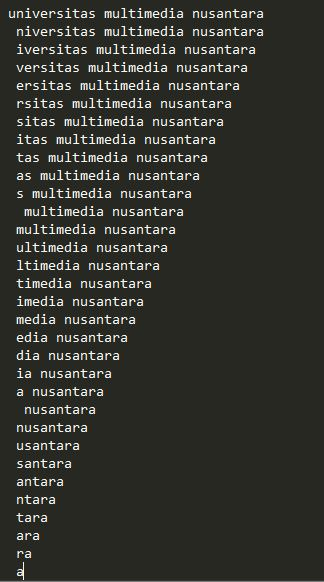
\includegraphics[width=0.25\textwidth]{gambar/perulangan}}
	\caption{Perulangan}
	\label{perulangan}
\end{figure}
Python dikenal sebagai bahasa pemograman interpreter, karena Python dieksekusi dengan sebuah interpreter. Satu hal yang telah kita ketahui bahwa bahasa pemograman Python adalah bahasa pemograman yang mudah dibaca dan terstruktur. Python sangat mementingkan indentasi, sehingga kita perlu melakukan indentasi secara konsisten. Indentasi tersebut dipermudah dengan penggunaan tombol Tab dan dimulai dari kolom pertama untuk setiap blok baru\cite{santoso2009bahasa}.
Python memiliki kelebihan lain yang sangat penting dibanding bahasa pemrograman yang terdahulu:
\begin{itemize}
\item Python merupakan open-source software, yang artinya ia dapat diperoleh secara gratis. Bahkan python sudah otomatis terinstall di Linux.
\item Python tersedia pada semua operating systems (OS) terkenal seperti Linux, Unix, Windows, dan MacOS. Suatu script python yang ditulis pada OS tertentu, dapat dijalankan di OS lain tapa ada modifikasi sedikitpun.
\item Python lebih mudah dipelajari sekaligus lebih mudah "‘dibaca"’ dibandingkan dengan bahasa pemrograman lainnya.
\item Python dan program ekstensinya mudah diinstall.
\end{itemize}
Python berdiri di atas landasan pondasi Java and C++. Hal-hal seperti classes, methods, inheritance, yang kerapkali diimplementasikan pada bahasa yang bersifat object-oriented, juga dapat diimplementasikan di python.\cite{suparno2013komputasi}

Secara umum, perulangan adalah blok kode yang dieksekusi berulang kali. Semua bahasa pemrograman menyediakan berbagai model struktur perulangan, seperti contohnya pada PHP ada while, for, dan foreach. Python juga menyediakan berbagai model tipe untuk menghandel perulangan. \par

Perintah perulangan di gunakan untuk mengulang pengeksekusian statemen-statemen hingga
berkali-kali sesuai dengan iterasi yang diinginkan. Dalam python, perintah untuk perulangan (loop)
adalah while dan for.

Secara umum, pernyataan pada bahasa pemrograman akan dieksekusi secara berurutan. Pernyataan pertama dalam sebuah fungsi dijalankan pertama, diikuti oleh yang kedua, dan seterusnya. Tetapi akan ada situasi dimana Anda harus menulis banyak kode, dimana kode tersebut sangat banyak. Jika dilakukan secara manual maka Anda hanya akan membuang-buang tenaga dengan menulis beratus-ratus bahkan beribu-ribu kode. Untuk itu Anda perlu menggunakan pengulangan di dalam bahasa pemrograman Python. \par

Di dalam bahasa pemrograman Python pengulangan dibagi menjadi 3 bagian, yaitu : 
\begin{itemize}
\item
While Loop 
\item
For Loop 
\item
Nested Loop 
\end{itemize} 
\vspace{\baselineskip}
\vspace{\baselineskip}
\vspace{12pt}


\subsection{While Loop}
Pengulangan While Loop di dalam bahasa pemrograman Python dieksesusi statement berkali-kali selama kondisi bernilai benar atau True. \par
\vspace{\baselineskip}
\vspace{\baselineskip}
Dibawah ini adalah contoh penggunaan pengulangan While Loop. \par
\vspace{\baselineskip}
\vspace{12pt}
Contoh penggunaan While Loop \par
\vspace{\baselineskip}
\vspace{\baselineskip}
\begin{verbatim}
count = 0 \par
while (count < 9): \par
 \$  \$  \$  \$ print ('The count is:', count) \par
 \$  \$  \$  \$ count = count + 1 \par
print ("Good bye!") \par
\end{verbatim}
\vspace{\baselineskip}
\vspace{\baselineskip}
\vspace{\baselineskip}
\vspace{12pt}

\subsection{For Loop}
Perulangan for disebut juga counted loop \(perulangan yang terhitung\)
Pengulangan for digunakan untuk pengulangan dengan muatan yang banyak\cite{van2007python}.
keistimewaan perulanga pada for adalah , perulangan dapat di hentikan pada saat kondisi tertentu. pada python, statemen for bekerja mengulang berbagai macam tipe data sekuensial seperti pada list, string dan tuple
Contohnya Seperti :
\begin{verbatim}
for a in range(0, 10):
	print a
\end{verbatim}
Hasil Outputnya :
\begin{verbatim}
python for.py
0
1
2
3
4
5
6
7
8
9
\end{verbatim}

Pengulangan For pada Python memiliki kemampuan untuk mengulangi item dari urutan apapun, seperti \$  \$list atau string. \par
\vspace{\baselineskip}
\vspace{\baselineskip}
Dibawah ini adalah contoh penggunaan pengulangan While Loop. \par
\vspace{\baselineskip}
\vspace{12pt}
Contoh pengulangan for sederhana \par
\vspace{\baselineskip}
angka = [1,2,3,4,5] \par
\vspace{\baselineskip}
for x in angka: \par
\vspace{\baselineskip}
 \$  \$  \$  \$ print(x) \par
\vspace{\baselineskip}
\vspace{\baselineskip}
Contoh pengulangan for \par
\vspace{\baselineskip}
buah = ["nanas", "apel", "jeruk"] \par
\vspace{\baselineskip}
for makanan in buah: \par
\vspace{\baselineskip}
 \$  \$  \$  \$ print(\"Saya suka makan\", makanan) \par
\vspace{\baselineskip}
\vspace{\baselineskip}
\vspace{12pt}

Looping artinya adalah pengulangan. Misalnya anda mendapat tugas untuk menghitung akar bilangan-bilangan dari 1 sampai 10. Ada 2 cara untuk menyelesaikan tugas tersebut, pertama, salinlah source-code berikut pada python editor lalu diberi nama looping01.py
\begin{enumerate}
\item from numpy import sqrt \# hanya function sqrt yang dipanggil
\item print sqrt(1)
\item print sqrt(2)
\item print sqrt(3)
\item print sqrt(4)
\item print sqrt(5)
\item print sqrt(6)
\item print sqrt(7)
\item print sqrt(8)
\item print sqrt(9)
\item print sqrt(10)
\end{enumerate}
Jalankan source-code di atas dengan menekan tombol F5, maka akan muncul hasil sebagai berikut :
\begin{enumerate}
\item 0
\item 41421356237
\item 73205080757
\item 0
\item 2360679775
\item 44948974278
\item 64575131106
\item 82842712475
\item 0
\item 16227766017
\end{enumerate}
Cara kedua dengan teknik looping, yaitu :
from numpy import sqrt
for i in range(1,10+1):
print sqrt(i)
Simpanlah source-code ini dengan nama looping02.py, lalu jalankan dengan F5, akan nampak
hasil yang sama yaitu
\begin{enumerate}
\item 0
\item 41421356237
\item 73205080757
\item 0
\item 2360679775
\item 44948974278
\item 64575131106
\item 82842712475
\item 0
\item 16227766017
\end{enumerate}

Mari sejenak kita bandingkan antara looping01.py dan looping02.py. Kedua source-code itu memiliki tujuan yang sama yaitu menghitung akar bilangan dari 1 sampai 10. Perbedaannya, looping01.py berisi 11 baris statemen, sedangkan looping02.py hanya 3 baris statemen. Coba cek
ukuran file-nya! Ukuran file looping01.py (di laptop saya) adalah 179 byte, sementara ukuran looping02.py adalah 72 byte. Dengan demikian dapat disimpulkan bahwa looping02.py lebih efisien dibanding looping01.py.\cite{suparno2013komputasi}

\subsection{Nested Loop}
Nested Loop (Perulangan Bertingkat) adalah semua tipe perulangan yang dapat dipakai di dalam perulangan yang lain. Jadi Perulangan for bisa dipakai di dalam for yang lain, perulangan for bisa berada didalam perulangan while, perulangan while bisa dipakai di dalam perulangan while yang lain, dan perulangan while bisa di dalam perulangan for. \par
\vspace{12pt}
Bahasa pemrograman Python memungkinkan penggunaan satu lingkaran di dalam loop lain. Bagian berikut menunjukkan beberapa contoh untuk menggambarkan konsep tersebut. \$  \$\vspace{\baselineskip}
\vspace{\baselineskip}
Dibawah ini adalah contoh penggunaan Nested Loop. \par

Contoh penggunaan Nested Loop : \par
\vspace{\baselineskip}
\vspace{\baselineskip}
i = 2 \par
\vspace{\baselineskip}
while(i < 100): \par
\vspace{\baselineskip}
 \$  \$  \$  \$ j = 2 \par
\vspace{\baselineskip}
 \$  \$  \$  \$ while(j <= (i/j)): \par
\vspace{\baselineskip}
 \$  \$  \$  \$  \$  \$  \$  \$ if not(i \$  \%  \$j): break \par
\vspace{\baselineskip}
 \$  \$  \$  \$  \$  \$  \$  \$ j = j + 1 \par
\vspace{\baselineskip}
 \$  \$  \$  \$ if (j > i/j) : print i, " is prime" \par
\vspace{\baselineskip}
 \$  \$  \$  \$ i = i + 1 \par
\vspace{\baselineskip}
\vspace{\baselineskip}
print "Good bye!" \par
\vspace{12pt}
\vspace{12pt}
Perhatikan contoh berikut ini:\vspace{\baselineskip}
\vspace{\baselineskip}
 \par
\vspace{12pt}
print ("1") \par
print ("2") \par
print ("3") \par
print ("4") \par
print ("5") \par
print ("6") \par
print ("7") \par
print ("8") \par
print ("9") \par
print ("10") \par
\vspace{12pt}
\vspace{\baselineskip}

Contoh program diatas adalah program untuk menampilkan angka 1 sampai dengan 10 tanpa perulangan. Tanpa menggunakan perulangan, programmer harus menuliskan semua statement diatas sehingga source code menjadi lebih banyak dan tidak efisien. Bayangkan kalau programmer disuruh menampilkan angka 1 sampai dengan 1000000 tanpa menggunakan perulangan\vspace{\baselineskip}
\vspace{\baselineskip}

Dengan menggunakan perulangan, source code lebih pendek dan efisien. Perhatikan contoh program untuk mencetak angka 1 sampai dengan 10 dengan menggunakan konsep perulangan di bawah ini.\vspace{\baselineskip}
\vspace{\baselineskip}
 \par
\vspace{12pt}

begin{verbatim}
i = 1 \par
while(i < 11): \par
~~~ print(i) \par
~~~ i = i+1 \par
end{verbatim}
\vspace{\baselineskip}

Bandingkan kedua program diatas, Mana yang lebih efisien? Mana yang lebih simple?\vspace{\baselineskip}
\vspace{\baselineskip}

Ada 3 macam bentuk perulangan pada Python, yaitu: \par
FOR Loop \par
WHILE Loop \par
dan Loop bersarang (Nested Loop) \par
\vspace{\baselineskip}

Selain membahas 3 bentuk perulangan diatas, tutorial ini juga membahas control perulangan, meliputi: \par
Break Statement \par
Continue Statement \par
dan Pass Statement \par
\vspace{\baselineskip}
\vspace{12pt}

\subsubsection{Contoh Penggunaan Nested Loop}
Format nested loop \(for di dalam for\)
\begin{verbatim}
For iterasi_var_1 in urutan_1:
	Statements_untuk_perulangan_for_yang_di_luar
...
For iterasi_var_1 in urutan_2:
	Statements_untuk_perulangan_for_yang_di_dalam
...
Statements_untuk_perulangan_for_yang_di_luar
...
\end{verbatim}

Format nested loop \(while di dalam while\)
\begin{verbatim}
While expressions:
	Statements_untuk_perulangan_while_yang_di_dalam
...
Statements_untuk_perulangan_whle_yang_di_luar
...
\end{verbatim}

Contoh :
\begin{verbatim}
X = int(input(“Masukkan jumlah bariss: “))
For i in range (x) :
	For j in range(i+1):
		Print(“*”, end=””)
	Print()
\end{verbatim}
Saat di Run Module maka :
Masukkan jumlah bariss: 5 \(inputkan 5\)
*
**
***
****
***** 
Muncul 5 baris isi bintang

\subsubsection{Nested Loop for Nested Data}
Disini kita memiliki list data dari murid-murid. Jadi, setiap murid memiliki nama yang dipasangkan dengan list subyek(mata pelajaran) yang mereka ambil. Dan akan mencetak setiap nama murid, dan jumlah dari subyek (mata pelajaran) yang mereka ambil
\begin{verbatim}
students = [
    ("John", ["TIK", "IPS"]),
    ("Vusi", ["Matematika", "TIK", "IPA"]),
    ("Jess", ["TIK", "Bahasa Indonesia", "Ekonomi", "Pendidikan Agama Islam"]),
    ("Sarah", ["Biologi", "Matematika", "Ekonomi", "Kimia"]),
    ("Zuki", ["Sosiologi", "Ekonomi", "Biologi", "Matematika", "Bahasa Inggris"])]

for (name, subjects) in students:
    print(name, "takes", len(subjects), "courses")
\end{verbatim}
Lalu, setelah dijalankan (run) maka akan tampil seperti ini:
John takes 2 courses
Vusi takes 3 courses
Jess takes 4 courses
Sarah takes 4 courses
Zuki takes 5 course

\subsection{FOR Loop}
FOR Loop digunakan untuk melakukan perulangan atau iterasi sampai batas atau range yang telah ditentukan.\vspace{\baselineskip}
\vspace{\baselineskip}
Dibawah ini adalah sintak dasar FOR Loop di Python.\vspace{\baselineskip}
\vspace{\baselineskip}
 \par
for iterating \$  \_  \$var in range: \par
~~ statements(s) \par
\vspace{\baselineskip}
Contoh Program\vspace{\baselineskip}
\vspace{\baselineskip}
Perhatikan contoh program For Loop pada Python:\vspace{\baselineskip}
\vspace{\baselineskip}
Contoh 1\vspace{\baselineskip}
\vspace{\baselineskip}
 \par
 \begin{equation}
 Program mencetak angka 1 s/d 10 
 \end{equation}
\vspace{12pt}
\begin{verbatim}
i = 10 \par
for i in range(10): \par
~~ print(i+1) \par
~~ i = i+1 \par
\end{verbatim}
\vspace{\baselineskip}
Fungsi \$  \$range() \$  \$biasanya digunakan sebagai counter pada perulangan bentuk For. range(10) artinya menampikan perulangan sebanyak 10 elemen.\vspace{\baselineskip}
\vspace{\baselineskip}
Apabila program diatas Anda jalankan, maka akan menampilkan angka 1 sampai dengan 10 seperti output di bawah ini:\vspace{\baselineskip}
\vspace{\baselineskip}
 \par
1 \par
2 \par
3 \par
4 \par
5 \par
6 \par
7 \par
8 \par
9 \par
10 \par
\vspace{\baselineskip}
Contoh 2\vspace{\baselineskip}
\vspace{\baselineskip}
 \par
 Program mencetak angka -1 s/d 8 \par
\vspace{12pt}
begin{verbatim}
i = 10 \par
for i in range(-10, 10, 2):  \$  \#  \$ range(range awal, range akhir, selisih) \par
~~ print(i) \par
end{verbatim}
\vspace{12pt}
\vspace{\baselineskip}
Perhatikan pada range(-10, 10, 2) artinya perulangan akan dimulai dari batas awal -10 sampai dengan batas akhir 10 dengan selisih 2.\vspace{\baselineskip}
\vspace{\baselineskip}
Apabila program diatas Anda jalankan, maka akan menampilkan output berikut ini:\vspace{\baselineskip}
\vspace{\baselineskip}
 \par
-10 \par
-8 \par
-6 \par
-4 \par
-2 \par
0 \par
2 \par
4 \par
6 \par
8 \par
\vspace{\baselineskip}
Contoh 3\vspace{\baselineskip}
\vspace{\baselineskip}
 \par
Program menampilkan huruf Belajar Python \par
for~huruf~in 'Belajar Python':    \par
~~ print (huruf) \par
\vspace{\baselineskip}
Apabila program diatas Anda jalankan, maka akan menghasilkan output berikut ini:\vspace{\baselineskip}
\vspace{\baselineskip}
 \par
B \par
e \par
l \par
a \par
j \par
a \par
r \par
  \par
P \par
y \par
t \par
h \par
o \par
n \par
\vspace{12pt}
Contoh 4\vspace{\baselineskip}
\vspace{\baselineskip}
Program berikut akan menampilkan perulangan dari list atau tupple.\vspace{\baselineskip}
\vspace{\baselineskip}
 \par
Program menampilkan huruf Belajar Python \par
\vspace{12pt}
begin{verbatim}
makanan = ['Pizza', 'Nasi Bebek',~ 'Rujak Buah'] \par
for makan in makanan: \par
~~ print (\"Makanan Favorit :\", makan) \par
end{verbatim}
\vspace{12pt}
Apabila program diatas Anda jalankan, maka akan menghasilkan output berikut ini:\vspace{\baselineskip}
\vspace{\baselineskip}
 \par
Makanan Favorit : Pizza \par
Makanan Favorit : Nasi Bebek \par
Makanan Favorit : Rujak Buah \par
\vspace{12pt}
\vspace{\baselineskip}
\vspace{12pt}
\subsection{While Loop}
While Loop akan menjalankan statemet selama kondisi terpenuhi (atau bernilai true).\vspace{\baselineskip}
\vspace{\baselineskip}
Di bawah ini adalah sintak dasar dari While Loop pada Python\vspace{\baselineskip}
\vspace{\baselineskip}
Contoh Program\vspace{\baselineskip}
\vspace{\baselineskip}
Coba Anda ketik program di bawah ini:\vspace{\baselineskip}
\vspace{\baselineskip}
 \par
Program mencetak angka 1 s/d 10 \par
\vspace{12pt}
begin{verbatim}
i = 1 \par
while(i < 11): \par
 print(i) \par
 i = i+1 \par
 end{verbatim}
\vspace{\baselineskip}

Apabila program diatas Anda jalankan, maka akan menghasilkan output seperti di bawah ini:\vspace{\baselineskip}
\vspace{\baselineskip}
 \par
1 \par
2 \par
3 \par
4 \par
5 \par
6 \par
7 \par
8 \par
9 \par
10 \par
\vspace{12pt}
\vspace{\baselineskip}
\vspace{12pt}
\subsection{Infinite Loop}
\vspace{\baselineskip}
Infinite Loop adalah kondisi perulangan, dimana statement akan dijalankan terus menerus tanpa berhenti. Akan berhenti kalau Anda menekan tombol CTRL+C.\vspace{\baselineskip}
\vspace{\baselineskip}
Di bawah ini contoh program Infinite Loop\vspace{\baselineskip}
\vspace{\baselineskip}
 \par
program menampilkan tulisan Python tanpa henti \par
\vspace{12pt}
flag = 1 \par
\vspace{12pt}
while (flag): print ("Python") \par
print ("Good bye!") \par
\vspace{12pt}
\vspace{\baselineskip}
\vspace{12pt}
\subsection{Nested Loop}
\vspace{\baselineskip}
Nested Loop secara sederhana adalah perulangan di dalam perulangan.\vspace{\baselineskip}
\vspace{\baselineskip}
Di bawah ini adalah sintak dasar Nested Loop pada Python:\vspace{\baselineskip}
\vspace{\baselineskip}
 \par
for iterating \$  \_  \$var in sequence: \par
~~ for iterating \$  \_  \$var in sequence: \par
~~~~~ statements(s) \par
~~ statements(s) \par
\vspace{\baselineskip}
atau yang menggunakan while loop\vspace{\baselineskip}
\vspace{\baselineskip}
 \par
while expression: \par
~~ while expression: \par
~~~~~ statement(s) \par
~~ statement(s) \par
\vspace{\baselineskip}
Contoh Program\vspace{\baselineskip}
\vspace{\baselineskip}
Di bawah ini adalah contoh program implementasi Nested Loop untuk mencetak bilangan prima dari 2 sampai 30.\vspace{\baselineskip}
\vspace{\baselineskip}
 \par
Program menampilkan bilangan prima dari 2 s/d 30 \par
\vspace{12pt}
\begin{verbatim}
i = 2 \par
while(i < 30): \par
~~ j = 2 \par
~~ while(j <= (i/j)): \par
~~~~~ if not(i \$  \%  \$j): break \par
~~~~~ j = j + 1 \par
~~ if (j > i/j) : print (i, \" adalah bilangan prima\") \par
~~ i = i + 1 \par
\end{verbatim}
\vspace{12pt}
print (\"Good bye!\") \par
\vspace{12pt}
\vspace{\baselineskip}
Apabila program diatas Anda jalankan, maka akan menampilkan output seperti di bawah ini.\vspace{\baselineskip}
\vspace{\baselineskip}
 \par
2~ adalah bilangan prima \par
3~ adalah bilangan prima \par
5~ adalah bilangan prima \par
7~ adalah bilangan prima \par
11~ adalah bilangan prima \par
13~ adalah bilangan prima \par
17~ adalah bilangan prima \par
19~ adalah bilangan prima \par
23~ adalah bilangan prima \par
29~ adalah bilangan prima \par
\vspace{12pt}
Pengulangan adalah salah satu hal penting yang ada di bahasa pemrograman. Pengulangan digunakan misalnya untuk meng-update \$  \$nama \$  \$file \$  \$yang cukup banyak jumlahnya, atau mengakses piksel satu persatu pada gambar. \par
Python memiliki tiga jenis pengulangan yang wajib Anda cermati untuk membuat sebuah aplikasi dengan Python. Pengulangan yang pertama adalah \$  \$while. Dengan menggunakan \$  \$while, Anda dapat membuat kondisi tertentu untuk menghentikan \$  \$while. Biasanya \$  \$while \$  \$digunakan untuk melakukan \$  \$loopingyang tidak pasti. Coba lihat contoh berikut (Anda dapat menulisnya dalam sebuah \$  \$file, kemudian eksekusi \$  \$file \$  \$tersebut di konsol): \par
begin{verbatim}
i = 0 \par
while True: \par
~~~ if i < 10: \par
~~~~~~~ print "Saat ini i bernilai: ", i \par
~~~~~~~ i = i + 1 \par
~~~ elif i >= 10: \par
~~~~~~~ break \par
end{verbatim}
\vspace{12pt}
Pada potongan kode diatas, \$  \$while \$  \$akan terus berputar selama i masih kurang dari 10. Jika sudah lebih dari 10 maka \$  \$while \$  \$akan berhenti. Pengulangan \$  \$whilejuga biasa digunakan di aplikasi konsol, untuk menahan \$  \$user \$  \$mengisikan semua input yang diperlukan dan baru akan berhenti setelah semua input dan proses interaksi berakhir. Jika kode diatas kita jalankan, maka \$  \$output-nya akan seperti ini: \par
\vspace{12pt}
Saat~ini i bernilai:  0 \par
Saat~ini i bernilai:  1 \par
Saat~ini i bernilai:  2 \par
Saat~ini i bernilai:  3 \par
Saat~ini i bernilai:  4 \par
Saat~ini i bernilai:  5 \par
Saat~ini i bernilai:  6 \par
Saat~ini i bernilai:  7 \par
Saat~ini i bernilai:  8 \par
Saat~ini i bernilai:  9 \par
\vspace{12pt}
Sekarang kita coba gunakan \$  \$for. Pengulangan \$  \$for \$  \$biasa digunakan untuk pengulangan yang sudah jelas banyaknya. Misal, Anda ingin mengulang sebuah pengulangan sampai 10 kali atau mengeluarkan semua hasil \$  \$query \$  \$dari \$  \$databasedi halaman HTML. Berikut ini adalah contoh kode untuk pengulangan \$  \$for: \par
for i in range(0, 10): \par
~~~ print i \par
Jika dijalankan maka kode diatas akan mengeluarkan \$  \$output \$  \$seperti ini: \par
\vspace{12pt}
0 \par
1 \par
2 \par
3 \par
4 \par
5 \par
6 \par
7 \par
8 \par
9 \par
Tidak hanya mengiterasi deretan angka, pengulangan \$  \$for \$  \$pun dapat Anda gunakan untuk mengulang sesuatu yang \$  \$iterable \$  \$seperti \$  \$list, \$  \$tuple, \$  \$dictionary, dan \$  \$iterable object \$  \$lainnya. Berikut ini kita ambil contoh dengan mengulang sebuah \$  \$list \$  \$yang berisi karakter anime Dragonball Super: \par
\vspace{12pt}
dragonball \$  \_  \$super \$  \_  \$character = [\"Son Goku\", \"Vegeta\", \"Beerus\", \"Trunks\", \"Whiz\", \"Champa\"] \par
for character in dragonball \$  \_  \$super \$  \_  \$character: \par
~~~ print character \par
\vspace{12pt}
Jika kita jalankan potongan kode tadi, maka \$  \$output-nya akan seperti berikut: \par
\vspace{12pt}
\begin{itemize}
\item
Son Goku
\item
Vegeta
\item
Beerus
\item
Trunks
\item
Whiz
\item
Champa
\item
For Loop
\end{itemize}
Seperti pada bahasa pemrograman lainnya, for loop sudah menjadi standar namun berbeda-beda tata cara penulisan nya di setiap pemrograman. \par
\vspace{12pt}
Sekarang kita langsung buat contoh di Python. \$  \$ \par
\vspace{12pt}
\vspace{12pt}
Contoh iterasi pada String  \par
\vspace{12pt}
\begin{verbatim}
for~n in 'Python':   \par
~~~ print 'Huruf :', n \par
\end{verbatim}
\vspace{12pt}
  \par
iterasi pada List biasa \par
\vspace{12pt}
mobil = ['sedan', 'truk', 'angkot']  \par
for p in mobil: \par
~~~ print 'Mobil :', mobil \par
\vspace{12pt}
\vspace{12pt}
iterasi pada list melalui index \par
for i in range(len(mobil)): \par
~~~ print 'Mobil :', mobil[i] \par
\vspace{12pt}
iterasi angka / range \par
\vspace{12pt}
for a in range(1,10): \par
~~~~ print "Angka :", a \par
~~~~ if(a == 5):  \$  \#  \$ditambah conditional \par
~~~~~~~~ print "Saya dapat angka : ",a \par
\vspace{12pt}
iterasi loop nested \par
for a in range(1,10): \par
~~~ for x in range(11,20): \par
~~~~~~~~b~=~a~* x      \par
~~~~~~~ print "Angka :", b \par
\vspace{12pt}
loop dgn break \par
for letter in 'Python': \par
~~ if letter == 'h': \par
~~~~~ break \par
~~ print 'Current Letter :', letter \par
\vspace{12pt}
print "Good job !!!" \par
\vspace{12pt}
\subsection{While Loop}
WHile dipakai untuk looping dimana iterasi akan dilakukan selama kondisi yang diberikan benar. While ini juga bisa di pakai untuk Infinite loop. \par
\vspace{12pt}
Contoh While \par
count = 0 \par
while count < 100: \par
 \$  \$  \$  \$  \$  \$print "Count ke : ", count \par
 \$  \$  \$  \$  \$  \$count = count + 1 \par
\vspace{12pt}
infinite loop \par
''' \par
Set loop ini untuk kondisi dimana suatu syarat tidak pernah TRUE \par
''' \par
\vspace{12pt}
setvar =1 \par
while setvar == 1 \par
 \$  \$  \$  \$ input = input \$  \_  \$raw("Masukan angka :") \par
 \$  \$  \$  \$ print "Angka anda : ", input \par
\vspace{12pt}
loop diatas akan berhenti jika anda stop manual misal dgn CTRL+C di terminal \par
''' \par
ELSE statement di while loop. di Python kita bisa set WHile loop lalu dikasih kondisi \par
''' \par
\begin{verbatim}
count = 0 \par
while count < 5: \par
 \$  \$  \$  \$  \$  \$print "count : ",count \par
 \$  \$  \$  \$  \$  \$count = count + 1 \par
else: \par
 \$  \$  \$  \$ print "Lihat yang masuk sini apa : ",count \par
 \end{verbatim}
\vspace{12pt}
while dgn break \par
angka~=~10~~~~~~    \par
while~angka~>~0:~~~~~~~~~~     \par
~~  \par
~~ print 'Angka :', angka \par
~~ angka = angka -1 \par
~~ if angka == 7: \par
~~~~~ break \par
\vspace{\baselineskip}
\vspace{12pt}
\vspace{12pt}

\subsection{Penggunaan loop dengan else statement}
Python mendukung untuk memiliki pernyataan lain yang terkait dengan pernyataan lingkaran
Jika else statement digunakan dengan for loop, pernyataan yang lain dijalankan saat loop telah habis mengulangi daftar.
Jika else statement digunakan dengan loop sementara, pernyataan yang lain dijalankan saat kondisinya menjadi salah.

\subsection{Middle-test loop}
Middle-test loop adalah sebuah perulangan yang akan mengeksekusi pada beberapa bagian body, kemudian akan melakukan pengujian exit berarti menguji dalam kondisi exit, lalu kemungkinan akan mengeksekusi beberapa bagian body lainnya. Disini dapat menggunakan while dan break secara bersama-sama. Terkadang kita membutuhkan looping dengan pengujian di tengah daripada pengujian di atas maupun di akhir.

\subsection{Penjelasan Penggunaan For Loop}
For loop secara tradisional digunakan saat Anda memiliki blok kode yang ingin Anda ulangi beberapa kali. Python untuk pernyataan iterates atas anggota urutan dalam urutan, mengeksekusi blok setiap waktu. Kontras untuk pernyataan dengan loop '' while '', digunakan bila suatu kondisi perlu diperiksa setiap iterasi, atau untuk mengulang blok kode selamanya.


%\chapter{Numbers}
%
NUMBERS \par
\vspace{12pt}
Nomor tipe data menyimpan nilai numerik. Mereka adalah tipe data yang tidak berubah, artinya mengubah nilai dari sejumlah hasil tipe data pada objek yang baru dialokasikan. \par
Nomor objek dibuat saat Anda memberikan nilai pada mereka. Contohnya – \par
\vspace{12pt}
var1 = 1 \par
var2 = 10 \par
Anda juga dapat menghapus referensi ke objek nomor dengan menggunakan del statement. Sintaks dari pernyataan del adalah - \par
\vspace{12pt}
del var1[,var2[,var3[....,varN]]]] \par
Anda dapat menghapus satu objek atau beberapa objek dengan menggunakan pernyataan del. Sebagai contoh: \par
\vspace{12pt}
del var \par
del var $  \_  $a, var $  \_  $b \par
Python mendukung empat jenis numerik yang berbeda – \par
\vspace{12pt}
 $ \bullet $ int (signed integers): Mereka sering disebut bilangan bulat atau int, bilangan bulat positif atau negatif tanpa titik desimal. \par
 $ \bullet $ panjang (bilangan bulat panjang): Juga disebut rindu, bilangan bulat adalah ukuran tak terbatas, ditulis seperti bilangan bulat dan diikuti huruf besar atau huruf kecil L. \par
 $ \bullet $ float (floating point real value): Disebut juga floats, mereka mewakili bilangan real dan ditulis dengan titik desimal membagi bilangan bulat dan bagian fraksional. Mengapung juga bisa dalam notasi ilmiah, dengan E atau e menunjukkan kekuatan 10 (2,5e2 = 2,5 x 102 = 250). \par
 $ \bullet $ kompleks (bilangan kompleks): berbentuk a + bJ, di mana a dan b mengapung dan J (atau j) mewakili akar kuadrat -1 (yang merupakan bilangan imajiner). Bagian sebenarnya dari bilangan tersebut adalah a, dan bagian imajinernya adalah b. Nomor kompleks tidak banyak digunakan dalam pemrograman Python. \par
CONTOH \par
Berikut adalah beberapa contoh angka \par
\vspace{12pt}
int \hspace*{0.5in} long \hspace*{0.5in} float \hspace*{0.5in} complex \par
10 \hspace*{0.5in} 51924361L \hspace*{0.5in} 0.0 \hspace*{0.5in} 3.14j \par
100 \hspace*{0.5in} -0x19323L \hspace*{0.5in} 15.20 \hspace*{0.5in} 45.j \par
-786 \hspace*{0.5in} 0122L \hspace*{0.5in} -21.9 \hspace*{0.5in} 9.322e-36j \par
080 \hspace*{0.5in} 0xDEFABCECBDAECBFBAEL \hspace*{0.5in} 32.3+e18 \hspace*{0.5in} .876j \par
-0490 \hspace*{0.5in} 535633629843L \hspace*{0.5in} -90. \hspace*{0.5in} -.6545+0J \par
-0x260 \hspace*{0.5in} -052318172735L \hspace*{0.5in} -32.54e100 \hspace*{0.5in} 3e+26J \par
0x69 \hspace*{0.5in} -4721885298529L \hspace*{0.5in} 70.2-E12 \hspace*{0.5in} 4.53e-7j \par
 $ \bullet $ Python memungkinkan Anda menggunakan huruf kecil L dengan panjang, namun disarankan agar Anda hanya menggunakan huruf besar L untuk menghindari kebingungan dengan nomor 1. Python menampilkan bilangan bulat panjang dengan huruf besar L. \par
 $ \bullet $ Nomor kompleks terdiri dari sepasang bilangan floating point asli yang ditandai dengan tanda + bj, di mana a adalah bagian sebenarnya dan b adalah bagian imajiner dari bilangan kompleks. \par
\vspace{12pt}
Konversi Tipe Jumlah \par
\vspace{12pt}
Python mengubah nomor secara internal dalam sebuah ekspresi yang mengandung tipe campuran untuk tipe umum untuk evaluasi. Tapi terkadang, Anda perlu memaksa nomor secara eksplisit dari satu jenis ke tipe lain untuk memenuhi persyaratan parameter operator atau fungsi. \par
\vspace{12pt}
 $ \bullet $ \hspace*{0.5in} Type int(x) to convert x to a plain integer. \par
 $ \bullet $ \hspace*{0.5in} Type long(x) to convert x to a long integer. \par
 $ \bullet $ \hspace*{0.5in} Type float(x) to convert x to a floating-point number. \par
 $ \bullet $ \hspace*{0.5in} Type complex(x) to convert x to a complex number with real part x and imaginary part zero. \par
 $ \bullet $ \hspace*{0.5in} Type complex(x, y) to convert x and y to a complex number with real part x and imaginary part y. x and y are numeric expressions \par
\vspace{12pt}
Fungsi Matematika \par
\vspace{12pt}
Python mencakup fungsi berikut yang melakukan perhitungan matematis. \par
\vspace{12pt}
Function \hspace*{0.5in} Returns ( description ) \par
abs(x) \par
The absolute value of x: the (positive) distance between x and zero. \par
ceil(x)  \par
The ceiling of x: the smallest integer not less than x \par
cmp(x, y) \par
-1 if x < y, 0 if x == y, or 1 if x > y  \par
exp(x)  \par
The exponential of x: ex  \par
fabs(x) \par
The absolute value of x. \par
floor(x)  \par
The floor of x: the largest integer not greater than x \par
log(x)  \par
The natural logarithm of x, for x> 0  \par
log10(x)  \par
The base-10 logarithm of x for x> 0 . \par
max(x1, x2,...)  \par
The largest of its arguments: the value closest to positive infinity  \par
min(x1, x2,...)  \par
The smallest of its arguments: the value closest to negative infinity  \par
modf(x)  \par
The fractional and integer parts of x in a two-item tuple. Both parts have the same sign as x. The integer part is returned as a float. \par
pow(x, y) \par
The value of x**y. \par
round(x [,n]) \par
x rounded to n digits from the decimal point. Python rounds away from zero as a tie-breaker: round(0.5) is 1.0 and round(-0.5) is -1.0. \par
sqrt(x)  \par
The square root of x for x > 0 \par
\vspace{12pt}
Fungsi Nomor Acak \par
\vspace{12pt}
Nomor acak digunakan untuk aplikasi permainan, simulasi, pengujian,  \par
\vspace{12pt}
keamanan, dan privasi. Python mencakup fungsi berikut yang umum digunakan. \par
\vspace{12pt}
Function \hspace*{0.5in} Description \par
choice(seq) \par
A random item from a list, tuple, or string. \par
randrange ([start,] stop [,step])  \par
A randomly selected element from range(start, stop, step) \par
random()  \par
A random float r, such that 0 is less than or equal to r and r is less than 1 \par
seed([x])  \par
Sets the integer starting value used in generating random numbers. Call this function before calling any other random module function. Returns None. \par
shuffle(lst)  \par
Randomizes the items of a list in place. Returns None. \par
uniform(x, y) \par
A random float r, such that x is less than or equal to r and r is less than y  \par
FUNGSI TRIGONOMETRIK \par
Python mencakup fungsi berikut yang melakukan perhitungan trigonometri. \par
\vspace{12pt}
Function \hspace*{0.5in} Description \par
acos(x) \par
Return the arc cosine of x, in radians. \par
asin(x) \par
Return the arc sine of x, in radians. \par
atan(x) \par
Return the arc tangent of x, in radians. \par
atan2(y, x) \par
Return atan(y / x), in radians.  \par
cos(x) \par
Return the cosine of x radians. \par
hypot(x, y) \par
Return the Euclidean norm, sqrt(x*x + y*y).  \par
sin(x) \par
Return the sine of x radians. \par
tan(x) \par
Return the tangent of x radians. \par
degrees(x) \par
Converts angle x from radians to degrees. \par
radians(x) \par
Converts angle x from degrees to radians. \par
\vspace{12pt}
Konstanta matematika \par
\vspace{12pt}
Modul ini juga mendefinisikan dua konstanta matematika – \par
\vspace{12pt}
Constants \hspace*{0.5in} Description \par
pi \hspace*{0.5in} The mathematical constant pi. \par
e \hspace*{0.5in} The mathematical constant e. \par
\vspace{12pt}
String adalah salah satu jenis yang paling populer dengan Python. Kita bisa membuatnya hanya dengan melampirkan karakter dalam tanda kutip. Python memperlakukan tanda petik tunggal sama dengan tanda kutip ganda. Membuat string semudah memberi nilai pada sebuah variabel. Misalnya – \par
\vspace{12pt}
var1 = 'Hello World!' \par
var2 = "Python Programming" \par
\vspace{12pt}
Mengakses Nilai dalam String \par
\vspace{12pt}
Python tidak mendukung tipe karakter; Ini diperlakukan sebagai string dengan panjang satu, sehingga juga dianggap sebagai substring. \par
Untuk mengakses substring, gunakan tanda kurung siku untuk mengiris beserta indeks atau indeks untuk mendapatkan substring Anda. Misalnya - \par
\vspace{12pt}
 $  \#  $!/usr/bin/python \par
\vspace{12pt}
var1 = 'Hello World!' \par
var2 = "Python Programming" \par
\vspace{12pt}
print "var1[0]: ", var1[0] \par
print "var2[1:5]: ", var2[1:5] \par
\vspace{12pt}
Bila kode diatas dieksekusi, maka menghasilkan hasil sebagai berikut - \par
\vspace{12pt}
var1[0]:~ H \par
var2[1:5]:~ ytho \par
Memperbarui String \par
\vspace{12pt}
Anda dapat "memperbarui" string yang ada dengan (kembali) menugaskan variabel ke string lain. Nilai baru dapat dikaitkan dengan nilai sebelumnya atau ke string yang sama sekali berbeda sama sekali. Misalnya - \par
\vspace{12pt}
 $  \#  $!/usr/bin/python \par
\vspace{12pt}
var1 = 'Hello World!' \par
\vspace{12pt}
print "Updated String :- ", var1[:6] + 'Python' \par
\vspace{12pt}
Bila kode diatas dieksekusi, maka menghasilkan hasil sebagai berikut - \par
\vspace{12pt}
Updated~String :-  Hello Python \par
\vspace{12pt}
Karakter melarikan diri \par
\vspace{12pt}
Tabel berikut adalah daftar karakter escape atau non-printable yang dapat diwakili dengan notasi backslash. \par
\vspace{12pt}
Karakter pelarian ditafsirkan; dalam satu dikutip serta dua kali mengutip string. \par
\vspace{12pt}
Backslash \par
notation \hspace*{0.5in} Hexadecimal \par
character \hspace*{0.5in} Description \par
 $  \textbackslash  $a \hspace*{0.5in} 0x07 \hspace*{0.5in} Bell or alert \par
 $  \textbackslash  $b \hspace*{0.5in} 0x08 \hspace*{0.5in} Backspace \par
 $  \textbackslash  $cx \hspace*{0.5in}   \hspace*{0.5in} Control-x \par
 $  \textbackslash  $C-x \hspace*{0.5in}   \hspace*{0.5in} Control-x \par
 $  \textbackslash  $e \hspace*{0.5in} 0x1b \hspace*{0.5in} Escape \par
 $  \textbackslash  $f \hspace*{0.5in} 0x0c \hspace*{0.5in} Formfeed \par
 $  \textbackslash  $M- $  \textbackslash  $C-x \hspace*{0.5in}   \hspace*{0.5in} Meta-Control-x \par
 $  \textbackslash  $n \hspace*{0.5in} 0x0a \hspace*{0.5in} Newline \par
 $  \textbackslash  $nnn \hspace*{0.5in}   \hspace*{0.5in} Octal notation, where n is in the range 0.7 \par
 $  \textbackslash  $r \hspace*{0.5in} 0x0d \hspace*{0.5in} Carriage return \par
 $  \textbackslash  $s \hspace*{0.5in} 0x20 \hspace*{0.5in} Space \par
 $  \textbackslash  $t \hspace*{0.5in} 0x09 \hspace*{0.5in} Tab \par
 $  \textbackslash  $v \hspace*{0.5in} 0x0b \hspace*{0.5in} Vertical tab \par
 $  \textbackslash  $x \hspace*{0.5in}   \hspace*{0.5in} Character x \par
 $  \textbackslash  $xnn \hspace*{0.5in}   \hspace*{0.5in} Hexadecimal notation, where n is in the range 0.9, a.f, or A.F \par
\vspace{12pt}
String Operator Khusus \par
\vspace{12pt}
Asumsikan variabel string memegang 'Halo' dan variabel b berisi 'Python', lalu – \par
\vspace{12pt}
Operator \hspace*{0.5in} Description \hspace*{0.5in} Example \par
+ \hspace*{0.5in} Concatenation - Adds values on either side of the operator \hspace*{0.5in} a + b will give HelloPython \par
* \hspace*{0.5in} Repetition - Creates new strings, concatenating multiple copies of the same string \hspace*{0.5in} a*2 will give -HelloHello \par
[] \hspace*{0.5in} Slice - Gives the character from the given index \hspace*{0.5in} a[1] will give e \par
[ : ] \hspace*{0.5in} Range Slice - Gives the characters from the given range \hspace*{0.5in} a[1:4] will give ell \par
in \hspace*{0.5in} Membership - Returns true if a character exists in the given string \hspace*{0.5in} H in a will give 1 \par
not in  \hspace*{0.5in} Membership - Returns true if a character does not exist in the given string \hspace*{0.5in} M not in a will give 1 \par
r/R \hspace*{0.5in} Raw String - Suppresses actual meaning of Escape characters. The syntax for raw strings is exactly the same as for normal strings with the exception of the raw string operator, the letter "r," which precedes the quotation marks. The "r" can be lowercase (r) or uppercase (R) and must be placed immediately preceding the first quote mark. \hspace*{0.5in} print r' $  \textbackslash  $n' prints  $  \textbackslash  $n and print R' $  \textbackslash  $n'prints  $  \textbackslash  $n \par
 $  \%  $ \hspace*{0.5in} Format - Performs String formatting \hspace*{0.5in} See at next section \par
\vspace{12pt}
\vspace{12pt}
Penyandian String Operator \par
Salah satu fitur Python yang paling keren adalah format string operator $  \%  $. Operator ini unik untuk string dan membuat paket memiliki fungsi dari keluarga printf C () C. Berikut adalah contoh sederhana - \par
 $  \#  $! / Usr / bin / python \par
\vspace{12pt}
Cetak "Nama saya $  \%  $ s dan beratnya adalah $  \%  $ d kg!"  $  \%  $ ('Zara', 21) \par
Bila kode diatas dieksekusi, maka menghasilkan hasil sebagai berikut - \par
Nama saya Zara dan beratnya adalah 21 kg! \par
Berikut adalah daftar lengkap simbol yang bisa digunakan bersamaan dengan $  \%  $ - \par
\vspace{12pt}
Format Symbol \hspace*{0.5in} Conversion \par
 $  \%  $c \hspace*{0.5in} character \par
 $  \%  $s \hspace*{0.5in} string conversion via str() prior to formatting \par
 $  \%  $i \hspace*{0.5in} signed decimal integer \par
 $  \%  $d \hspace*{0.5in} signed decimal integer \par
 $  \%  $u \hspace*{0.5in} unsigned decimal integer \par
 $  \%  $o \hspace*{0.5in} octal integer \par
 $  \%  $x \hspace*{0.5in} hexadecimal integer (lowercase letters) \par
 $  \%  $X \hspace*{0.5in} hexadecimal integer (UPPERcase letters) \par
 $  \%  $e \hspace*{0.5in} exponential notation (with lowercase 'e') \par
 $  \%  $E \hspace*{0.5in} exponential notation (with UPPERcase 'E') \par
 $  \%  $f \hspace*{0.5in} floating point real number \par
 $  \%  $g \hspace*{0.5in} the shorter of  $  \%  $f and  $  \%  $e \par
 $  \%  $G \hspace*{0.5in} the shorter of  $  \%  $f and  $  \%  $E \par
\vspace{12pt}
Simbol dan fungsionalitas pendukung lainnya tercantum dalam tabel berikut – \par
\vspace{12pt}
Symbol \hspace*{0.5in} Functionality \par
* \hspace*{0.5in} argument specifies width or precision \par
- \hspace*{0.5in} left justification \par
+ \hspace*{0.5in} display the sign \par
<sp> \hspace*{0.5in} leave a blank space before a positive number \par
 $  \#  $ \hspace*{0.5in} add the octal leading zero ( '0' ) or hexadecimal leading '0x' or '0X', depending on whether 'x' or 'X' were used. \par
0 \hspace*{0.5in} pad from left with zeros (instead of spaces) \par
 $  \%  $ \hspace*{0.5in} ' $  \%  $ $  \%  $' leaves you with a single literal ' $  \%  $' \par
(var) \hspace*{0.5in} mapping variable (dictionary arguments) \par
m.n. \hspace*{0.5in} m is the minimum total width and n is the number of digits to display after the decimal point (if appl.) \par
\vspace{12pt}
Triple Quotes \par
\vspace{12pt}
Tiga tanda kutip Python hadir untuk menyelamatkannya dengan membiarkan string memanjang banyak baris, termasuk kata kunci NEWLINEs, TABs, dan karakter khusus lainnya. \par
Sintaks untuk triple quotes terdiri dari tiga tanda kutip tunggal atau ganda berturut-turut. \par
 $  \#  $! / Usr / bin / python \par
\vspace{12pt}
para $  \_  $str = "" "ini adalah string panjang yang terdiri dari \par
Beberapa baris dan karakter yang tidak dapat dicetak seperti \par
TAB ( $  \textbackslash  $ t) dan mereka akan muncul seperti itu saat ditampilkan. \par
NEWLINEs dalam string, apakah secara eksplisit diberikan seperti \par
Ini dalam tanda kurung [ $  \textbackslash  $ n], atau hanya NEWLINE di dalamnya \par
tugas variabel juga akan muncul. \par
"" " \par
Cetak para $  \_  $str \par
Bila kode diatas dieksekusi, maka hasilnya akan menghasilkan hasil berikut. Perhatikan bagaimana setiap karakter khusus telah diubah menjadi bentuk cetaknya, sampai ke NEWLINE terakhir di akhir string antara "up". Dan menutup tanda kutip tiga kali. Perhatikan juga bahwa NEWLINEs terjadi baik dengan carriage return yang eksplisit di akhir baris atau kode escape-nya ( $  \textbackslash  $ n) - \par
Ini adalah string panjang yang terdiri dari \par
beberapa baris dan karakter yang tidak dapat dicetak seperti \par
TAB () dan mereka akan muncul seperti itu saat ditampilkan. \par
NEWLINEs dalam string, apakah secara eksplisit diberikan seperti \par
ini dalam tanda kurung [ \par
 ], atau hanya NEWLINE di dalamnya \par
tugas variabel juga akan muncul. \par
String mentah tidak memperlakukan garis miring terbalik sebagai karakter spesial sama sekali. Setiap karakter yang Anda masukkan ke dalam string mentah tetap seperti yang Anda tulis - \par
 $  \#  $! / Usr / bin / python \par
\vspace{12pt}
cetak 'C:  $  \textbackslash  $ $  \textbackslash  $ tempat' \par
Bila kode diatas dieksekusi, maka menghasilkan hasil sebagai berikut - \par
C: di mana-mana \par
Sekarang mari kita gunakan string mentah. Kami akan mengutarakan ekspresi 'sebagai berikut - \par
 $  \#  $! / Usr / bin / python \par
\vspace{12pt}
Cetak r'C:  $  \textbackslash  $ $  \textbackslash  $ tempat ' \par
Bila kode diatas dieksekusi, maka menghasilkan hasil sebagai berikut - \par
C: tidak di mana-mana \par
String Unicode \par
String normal dengan Python disimpan secara internal sebagai 8-bit ASCII, sedangkan string Unicode disimpan sebagai Unicode 16-bit. Hal ini memungkinkan untuk serangkaian karakter yang lebih bervariasi, termasuk karakter khusus dari kebanyakan bahasa di dunia. Saya akan membatasi perlakuan saya terhadap string Unicode sebagai berikut - \par
 $  \#  $! / Usr / bin / python \par
\vspace{12pt}
cetak u'Hello, dunia! ' \par
Bila kode diatas dieksekusi, maka menghasilkan hasil sebagai berikut - \par
Halo Dunia! \par
Seperti yang bisa Anda lihat, senar Unicode menggunakan awalan Anda, sama seperti senar biasa menggunakan awalan r. \par
Metode String Terpadu \par
Python menyertakan metode built-in berikut untuk memanipulasi string – \par
\vspace{12pt}
SN \hspace*{0.5in} Methods with Description \par
1 \hspace*{0.5in} capitalize() \par
Capitalizes first letter of string \par
2 \hspace*{0.5in} center(width, fillchar) \par
\vspace{12pt}
Returns a space-padded string with the original string centered to a total of width columns. \par
3 \hspace*{0.5in} count(str, beg= 0,end=len(string)) \par
\vspace{12pt}
Counts how many times str occurs in string or in a substring of string if starting index beg and ending index end are given. \par
4 \hspace*{0.5in} decode(encoding='UTF-8',errors='strict') \par
\vspace{12pt}
Decodes the string using the codec registered for encoding. encoding defaults to the default string encoding. \par
5 \hspace*{0.5in} encode(encoding='UTF-8',errors='strict') \par
\vspace{12pt}
Returns encoded string version of string; on error, default is to raise a ValueError unless errors is given with 'ignore' or 'replace'. \par
6 \hspace*{0.5in} endswith(suffix, beg=0, end=len(string)) \par
Determines if string or a substring of string (if starting index beg and ending index end are given) ends with suffix; returns true if so and false otherwise. \par
7 \hspace*{0.5in} expandtabs(tabsize=8) \par
\vspace{12pt}
Expands tabs in string to multiple spaces; defaults to 8 spaces per tab if tabsize not provided. \par
8 \hspace*{0.5in} find(str, beg=0 end=len(string)) \par
\vspace{12pt}
Determine if str occurs in string or in a substring of string if starting index beg and ending index end are given returns index if found and -1 otherwise. \par
9 \hspace*{0.5in} index(str, beg=0, end=len(string)) \par
\vspace{12pt}
Same as find(), but raises an exception if str not found. \par
10 \hspace*{0.5in} isalnum() \par
\vspace{12pt}
Returns true if string has at least 1 character and all characters are alphanumeric and false otherwise. \par
11 \hspace*{0.5in} isalpha() \par
\vspace{12pt}
Returns true if string has at least 1 character and all characters are alphabetic and false otherwise. \par
12 \hspace*{0.5in} isdigit() \par
\vspace{12pt}
Returns true if string contains only digits and false otherwise. \par
13 \hspace*{0.5in} islower() \par
\vspace{12pt}
Returns true if string has at least 1 cased character and all cased characters are in lowercase and false otherwise. \par
14 \hspace*{0.5in} isnumeric() \par
\vspace{12pt}
Returns true if a unicode string contains only numeric characters and false otherwise. \par
15 \hspace*{0.5in} isspace() \par
\vspace{12pt}
Returns true if string contains only whitespace characters and false otherwise. \par
16 \hspace*{0.5in} istitle() \par
\vspace{12pt}
Returns true if string is properly "titlecased" and false otherwise. \par
17 \hspace*{0.5in} isupper() \par
\vspace{12pt}
Returns true if string has at least one cased character and all cased characters are in uppercase and false otherwise. \par
18 \hspace*{0.5in} join(seq) \par
\vspace{12pt}
Merges (concatenates) the string representations of elements in sequence seq into a string, with separator string. \par
19 \hspace*{0.5in} len(string) \par
\vspace{12pt}
Returns the length of the string \par
20 \hspace*{0.5in} ljust(width[, fillchar]) \par
\vspace{12pt}
Returns a space-padded string with the original string left-justified to a total of width columns. \par
21 \hspace*{0.5in} lower() \par
\vspace{12pt}
Converts all uppercase letters in string to lowercase. \par
22 \hspace*{0.5in} lstrip() \par
\vspace{12pt}
Removes all leading whitespace in string. \par
23 \hspace*{0.5in} maketrans() \par
\vspace{12pt}
Returns a translation table to be used in translate function. \par
24 \hspace*{0.5in} max(str) \par
\vspace{12pt}
Returns the max alphabetical character from the string str. \par
25 \hspace*{0.5in} min(str) \par
\vspace{12pt}
Returns the min alphabetical character from the string str. \par
26 \hspace*{0.5in} replace(old, new [, max]) \par
\vspace{12pt}
Replaces all occurrences of old in string with new or at most max occurrences if max given. \par
27 \hspace*{0.5in} rfind(str, beg=0,end=len(string)) \par
\vspace{12pt}
Same as find(), but search backwards in string. \par
28 \hspace*{0.5in} rindex( str, beg=0, end=len(string)) \par
\vspace{12pt}
Same as index(), but search backwards in string. \par
29 \hspace*{0.5in} rjust(width,[, fillchar]) \par
\vspace{12pt}
Returns a space-padded string with the original string right-justified to a total of width columns. \par
30 \hspace*{0.5in} rstrip() \par
\vspace{12pt}
Removes all trailing whitespace of string. \par
31 \hspace*{0.5in} split(str="", num=string.count(str)) \par
\vspace{12pt}
Splits string according to delimiter str (space if not provided) and returns list of substrings; split into at most num substrings if given. \par
32 \hspace*{0.5in} splitlines( num=string.count(' $  \textbackslash  $n')) \par
\vspace{12pt}
Splits string at all (or num) NEWLINEs and returns a list of each line with NEWLINEs removed. \par
33 \hspace*{0.5in} startswith(str, beg=0,end=len(string)) \par
\vspace{12pt}
Determines if string or a substring of string (if starting index beg and ending index end are given) starts with substring str; returns true if so and false otherwise. \par
34 \hspace*{0.5in} strip([chars]) \par
\vspace{12pt}
Performs both lstrip() and rstrip() on string \par
35 \hspace*{0.5in} swapcase() \par
\vspace{12pt}
Inverts case for all letters in string. \par
36 \hspace*{0.5in} title() \par
\vspace{12pt}
Returns "titlecased" version of string, that is, all words begin with uppercase and the rest are lowercase. \par
37 \hspace*{0.5in} translate(table, deletechars="") \par
\vspace{12pt}
Translates string according to translation table str(256 chars), removing those in the del string. \par
38 \hspace*{0.5in} upper() \par
\vspace{12pt}
Converts lowercase letters in string to uppercase. \par
39 \hspace*{0.5in} zfill (width) \par
\vspace{12pt}
Returns original string leftpadded with zeros to a total of width characters; intended for numbers, zfill() retains any sign given (less one zero). \par
40 \hspace*{0.5in} isdecimal() \par
\vspace{12pt}
Returns true if a unicode string contains only decimal characters and false otherwise. \par
\vspace{12pt}
9.1.2.2. Implementing the arithmetic operations \par
We want to implement the arithmetic operations so that mixed-mode operations either call an implementation whose author knew about the types of both arguments, or convert both to the nearest built in type and do the operation there. For subtypes of Integral, this means that  $  \_  $ $  \_  $add $  \_  $ $  \_  $() and  $  \_  $ $  \_  $radd $  \_  $ $  \_  $() should be defined as: \par
class MyIntegral(Integral): \par
\vspace{12pt}
~~~ def  $  \_  $ $  \_  $add $  \_  $ $  \_  $(self, other): \par
~~~~~~~ if isinstance(other, MyIntegral): \par
~~~~~~~~~~~ return do $  \_  $my $  \_  $adding $  \_  $stuff(self, other) \par
~~~~~~~ elif isinstance(other, OtherTypeIKnowAbout): \par
~~~~~~~~~~~ return do $  \_  $my $  \_  $other $  \_  $adding $  \_  $stuff(self, other) \par
~~~~~~~ else: \par
~~~~~~~~~~~ return NotImplemented \par
\vspace{12pt}
~~~ def  $  \_  $ $  \_  $radd $  \_  $ $  \_  $(self, other): \par
~~~~~~~ if isinstance(other, MyIntegral): \par
~~~~~~~~~~~ return do $  \_  $my $  \_  $adding $  \_  $stuff(other, self) \par
~~~~~~~ elif isinstance(other, OtherTypeIKnowAbout): \par
~~~~~~~~~~~ return do $  \_  $my $  \_  $other $  \_  $adding $  \_  $stuff(other, self) \par
~~~~~~~ elif isinstance(other, Integral): \par
~~~~~~~~~~~ return int(other) + int(self) \par
~~~~~~~ elif isinstance(other, Real): \par
~~~~~~~~~~~ return float(other) + float(self) \par
~~~~~~~ elif isinstance(other, Complex): \par
~~~~~~~~~~~ return complex(other) + complex(self) \par
~~~~~~~ else: \par
~~~~~~~~~~~ return NotImplemented \par
There are 5 different cases for a mixed-type operation on subclasses of Complex. I’ll refer to all of the above code that doesn’t refer to MyIntegral and OtherTypeIKnowAbout as  $ " $boilerplate $ " $. a will be an instance of A, which is a subtype of Complex (a : A <: Complex), and b : B <: Complex. I’ll consider a + b: \par
1. \hspace*{0.5in} If A defines an  $  \_  $ $  \_  $add $  \_  $ $  \_  $() which accepts b, all is well. \par
2. \hspace*{0.5in} If A falls back to the boilerplate code, and it were to return a value from  $  \_  $ $  \_  $add $  \_  $ $  \_  $(), we’d miss the possibility that B defines a more intelligent  $  \_  $ $  \_  $radd $  \_  $ $  \_  $(), so the boilerplate should return NotImplemented from  $  \_  $ $  \_  $add $  \_  $ $  \_  $(). (Or A may not implement  $  \_  $ $  \_  $add $  \_  $ $  \_  $() at all.) \par
3. \hspace*{0.5in} Then B’s  $  \_  $ $  \_  $radd $  \_  $ $  \_  $() gets a chance. If it accepts a, all is well. \par
4. \hspace*{0.5in} If it falls back to the boilerplate, there are no more possible methods to try, so this is where the default implementation should live. \par
5. \hspace*{0.5in} If B <: A, Python tries B. $  \_  $ $  \_  $radd $  \_  $ $  \_  $ before A. $  \_  $ $  \_  $add $  \_  $ $  \_  $. This is ok, because it was implemented with knowledge of A, so it can handle those instances before delegating to Complex. \par
If A <: Complex and B <: Real without sharing any other knowledge, then the appropriate shared operation is the one involving the built in complex, and both  $  \_  $ $  \_  $radd $  \_  $ $  \_  $() s land there, so a+b == b+a. \par
Because most of the operations on any given type will be very similar, it can be useful to define a helper function which generates the forward and reverse instances of any given operator. For example, fractions.Fraction uses: \par
def  $  \_  $operator $  \_  $fallbacks(monomorphic $  \_  $operator, fallback $  \_  $operator): \par
~~~ def forward(a, b): \par
~~~~~~~ if isinstance(b, (int, long, Fraction)): \par
~~~~~~~~~~~ return monomorphic $  \_  $operator(a, b) \par
~~~~~~~ elif isinstance(b, float): \par
~~~~~~~~~~~ return fallback $  \_  $operator(float(a), b) \par
~~~~~~~ elif isinstance(b, complex): \par
~~~~~~~~~~~ return fallback $  \_  $operator(complex(a), b) \par
~~~~~~~ else: \par
~~~~~~~~~~~ return NotImplemented \par
~~~ forward. $  \_  $ $  \_  $name $  \_  $ $  \_  $ = ' $  \_  $ $  \_  $' + fallback $  \_  $operator. $  \_  $ $  \_  $name $  \_  $ $  \_  $ + ' $  \_  $ $  \_  $' \par
~~~ forward. $  \_  $ $  \_  $doc $  \_  $ $  \_  $ = monomorphic $  \_  $operator. $  \_  $ $  \_  $doc $  \_  $ $  \_  $ \par
\vspace{12pt}
~~~ def reverse(b, a): \par
~~~~~~~ if isinstance(a, Rational): \par
~~~~~~~~~~~  $  \#  $ Includes ints. \par
~~~~~~~~~~~ return monomorphic $  \_  $operator(a, b) \par
~~~~~~~ elif isinstance(a, numbers.Real): \par
~~~~~~~~~~~ return fallback $  \_  $operator(float(a), float(b)) \par
~~~~~~~ elif isinstance(a, numbers.Complex): \par
~~~~~~~~~~~ return fallback $  \_  $operator(complex(a), complex(b)) \par
~~~~~~~ else: \par
~~~~~~~~~~~ return NotImplemented \par
~~~ reverse. $  \_  $ $  \_  $name $  \_  $ $  \_  $ = ' $  \_  $ $  \_  $r' + fallback $  \_  $operator. $  \_  $ $  \_  $name $  \_  $ $  \_  $ + ' $  \_  $ $  \_  $' \par
~~~ reverse. $  \_  $ $  \_  $doc $  \_  $ $  \_  $ = monomorphic $  \_  $operator. $  \_  $ $  \_  $doc $  \_  $ $  \_  $ \par
\vspace{12pt}
~~~ return forward, reverse \par
\vspace{12pt}
def  $  \_  $add(a, b): \par
~~~ """a + b""" \par
~~~ return Fraction(a.numerator * b.denominator + \par
~~~~~~~~~~~~~~~~~~~ b.numerator * a.denominator, \par
~~~~~~~~~~~~~~~~~~~ a.denominator * b.denominator) \par
\vspace{12pt}
 $  \_  $ $  \_  $add $  \_  $ $  \_  $,  $  \_  $ $  \_  $radd $  \_  $ $  \_  $ =  $  \_  $operator $  \_  $fallbacks( $  \_  $add, operator.add) \par
\vspace{12pt}
 $  \#  $ ... \par
\vspace{12pt}



%\chapter{Strings}
% 
STRING \par
String adalah salah satu jenis yang paling populer dengan Python. Kita bisa membuatnya hanya dengan melampirkan karakter dalam tanda kutip. Python memperlakukan tanda petik tunggal sama dengan tanda kutip ganda. Membuat string semudah memberi nilai pada sebuah variabel. Misalnya - \par
\vspace{12pt}
var1 = 'Hello World!' \par
var2 = "Python Programming" \par
\vspace{12pt}
Mengakses Nilai dalam String \par
Python tidak mendukung tipe karakter; Ini diperlakukan sebagai string dengan panjang satu, sehingga juga dianggap sebagai substring. \par
Untuk mengakses substring, gunakan tanda kurung siku untuk mengiris beserta indeks atau indeks untuk mendapatkan substring Anda. Misalnya - \par
\vspace{12pt}
 $  \#  $!/usr/bin/python \par
\vspace{12pt}
var1 = 'Hello World!' \par
var2 = "Python Programming" \par
\vspace{12pt}
print "var1[0]: ", var1[0] \par
print "var2[1:5]: ", var2[1:5] \par
\vspace{12pt}
Bila kode diatas dieksekusi, maka menghasilkan hasil sebagai berikut - \par
\vspace{12pt}
var1[0]:~ H \par
var2[1:5]:~ ytho \par
\vspace{12pt}
 $  \#  $!/usr/bin/python \par
\vspace{12pt}
Memperbarui String \par
Anda dapat "memperbarui" string yang ada dengan (kembali) menugaskan variabel ke string lain. Nilai baru dapat dikaitkan dengan nilai sebelumnya atau ke string yang sama sekali berbeda sama sekali. Misalnya - \par
\vspace{12pt}
\vspace{12pt}
var1 = 'Hello World!' \par
\vspace{12pt}
print "Updated String :- ", var1[:6] + 'Python' \par
\vspace{12pt}
Bila kode diatas dieksekusi, maka menghasilkan hasil sebagai berikut - \par
\vspace{12pt}
Updated~String :-  Hello Python \par
\vspace{12pt}
Karakter melarikan diri \par
\vspace{12pt}
Tabel berikut adalah daftar karakter escape atau non-printable yang dapat diwakili dengan notasi backslash. \par
Karakter pelarian ditafsirkan; dalam satu dikutip serta dua kali mengutip string. \par
\vspace{12pt}
Backslash \par
notation \hspace*{0.5in} Hexadecimal \par
character \hspace*{0.5in} Description \par
 $  \textbackslash  $a \hspace*{0.5in} 0x07 \hspace*{0.5in} Bell or alert \par
 $  \textbackslash  $b \hspace*{0.5in} 0x08 \hspace*{0.5in} Backspace \par
 $  \textbackslash  $cx \hspace*{0.5in}   \hspace*{0.5in} Control-x \par
 $  \textbackslash  $C-x \hspace*{0.5in}   \hspace*{0.5in} Control-x \par
 $  \textbackslash  $e \hspace*{0.5in} 0x1b \hspace*{0.5in} Escape \par
 $  \textbackslash  $f \hspace*{0.5in} 0x0c \hspace*{0.5in} Formfeed \par
 $  \textbackslash  $M- $  \textbackslash  $C-x \hspace*{0.5in}   \hspace*{0.5in} Meta-Control-x \par
 $  \textbackslash  $n \hspace*{0.5in} 0x0a \hspace*{0.5in} Newline \par
 $  \textbackslash  $nnn \hspace*{0.5in}   \hspace*{0.5in} Octal notation, where n is in the range 0.7 \par
 $  \textbackslash  $r \hspace*{0.5in} 0x0d \hspace*{0.5in} Carriage return \par
 $  \textbackslash  $s \hspace*{0.5in} 0x20 \hspace*{0.5in} Space \par
 $  \textbackslash  $t \hspace*{0.5in} 0x09 \hspace*{0.5in} Tab \par
 $  \textbackslash  $v \hspace*{0.5in} 0x0b \hspace*{0.5in} Vertical tab \par
 $  \textbackslash  $x \hspace*{0.5in}   \hspace*{0.5in} Character x \par
 $  \textbackslash  $xnn \hspace*{0.5in}   \hspace*{0.5in} Hexadecimal notation, where n is in the range 0.9, a.f, or A.F \par
\vspace{12pt}
String Operator Khusus \par
\vspace{12pt}
Asumsikan variabel string memegang 'Halo' dan variabel b berisi 'Python',  \par
lalu – \par
\vspace{12pt}
Operator \hspace*{0.5in} Description \hspace*{0.5in} Example \par
+ \hspace*{0.5in} Concatenation - Adds values on either side of the operator \hspace*{0.5in} a + b will give HelloPython \par
* \hspace*{0.5in} Repetition - Creates new strings, concatenating multiple copies of the same string \hspace*{0.5in} a*2 will give -HelloHello \par
[] \hspace*{0.5in} Slice - Gives the character from the given index \hspace*{0.5in} a[1] will give e \par
[ : ] \hspace*{0.5in} Range Slice - Gives the characters from the given range \hspace*{0.5in} a[1:4] will give ell \par
in \hspace*{0.5in} Membership - Returns true if a character exists in the given string \hspace*{0.5in} H in a will give 1 \par
not in  \hspace*{0.5in} Membership - Returns true if a character does not exist in the given string \hspace*{0.5in} M not in a will give 1 \par
r/R \hspace*{0.5in} Raw String - Suppresses actual meaning of Escape characters. The syntax for raw strings is exactly the same as for normal strings with the exception of the raw string operator, the letter "r," which precedes the quotation marks. The "r" can be lowercase (r) or uppercase (R) and must be placed immediately preceding the first quote mark. \hspace*{0.5in} print r' $  \textbackslash  $n' prints  $  \textbackslash  $n and print R' $  \textbackslash  $n'prints  $  \textbackslash  $n \par
 $  \%  $ \hspace*{0.5in} Format - Performs String formatting \hspace*{0.5in} See at next section \par
\vspace{12pt}
Penyandian String Operator \par
\vspace{12pt}
Salah satu fitur Python yang paling keren adalah format string operator $  \%  $. Operator ini unik untuk string dan membuat paket memiliki fungsi dari keluarga printf C () C. Berikut adalah contoh sederhana - \par
\vspace{12pt}
 $  \#  $!/usr/bin/python \par
\vspace{12pt}
print "My name is  $  \%  $s and weight is  $  \%  $d kg!"  $  \%  $ ('Zara', 21)  \par
\vspace{12pt}
Bila kode diatas dieksekusi, maka menghasilkan hasil sebagai berikut - \par
\vspace{12pt}
My name is Zara and weight is 21 kg! \par
Here is the list of complete set of symbols which can be used along with  $  \%  $  $ - $ \par
Format Symbol \hspace*{0.5in} Conversion \par
 $  \%  $c \hspace*{0.5in} character \par
 $  \%  $s \hspace*{0.5in} string conversion via str() prior to formatting \par
 $  \%  $i \hspace*{0.5in} signed decimal integer \par
 $  \%  $d \hspace*{0.5in} signed decimal integer \par
 $  \%  $u \hspace*{0.5in} unsigned decimal integer \par
 $  \%  $o \hspace*{0.5in} octal integer \par
 $  \%  $x \hspace*{0.5in} hexadecimal integer (lowercase letters) \par
 $  \%  $X \hspace*{0.5in} hexadecimal integer (UPPERcase letters) \par
 $  \%  $e \hspace*{0.5in} exponential notation (with lowercase 'e') \par
 $  \%  $E \hspace*{0.5in} exponential notation (with UPPERcase 'E') \par
 $  \%  $f \hspace*{0.5in} floating point real number \par
 $  \%  $g \hspace*{0.5in} the shorter of  $  \%  $f and  $  \%  $e \par
 $  \%  $G \hspace*{0.5in} the shorter of  $  \%  $f and  $  \%  $E \par
Other supported symbols and functionality are listed in the following table  $ - $ \par
Symbol \hspace*{0.5in} Functionality \par
* \hspace*{0.5in} argument specifies width or precision \par
- \hspace*{0.5in} left justification \par
+ \hspace*{0.5in} display the sign \par
<sp> \hspace*{0.5in} leave a blank space before a positive number \par
 $  \#  $ \hspace*{0.5in} add the octal leading zero ( '0' ) or hexadecimal leading '0x' or '0X', depending on whether 'x' or 'X' were used. \par
0 \hspace*{0.5in} pad from left with zeros (instead of spaces) \par
 $  \%  $ \hspace*{0.5in} ' $  \%  $ $  \%  $' leaves you with a single literal ' $  \%  $' \par
(var) \hspace*{0.5in} mapping variable (dictionary arguments) \par
m.n. \hspace*{0.5in} m is the minimum total width and n is the number of digits to display after the decimal point (if appl.) \par
\vspace{12pt}
Triple Quotes \par
\vspace{12pt}
Tiga tanda kutip Python hadir untuk menyelamatkannya dengan membiarkan string memanjang banyak baris, termasuk kata kunci NEWLINEs, TABs, dan karakter khusus lainnya. \par
Sintaks untuk triple quotes terdiri dari tiga tanda kutip tunggal atau ganda berturut-turut. \par
\vspace{12pt}
 $  \#  $!/usr/bin/python \par
\vspace{12pt}
para $  \_  $str = "" "ini adalah string panjang yang terdiri dari \par
beberapa baris dan karakter yang tidak dapat dicetak seperti \par
TAB ( $  \textbackslash  $ t) dan mereka akan muncul seperti itu saat ditampilkan. \par
NEWLINEs dalam string, apakah secara eksplisit diberikan seperti \par
Ini dalam tanda kurung [ $  \textbackslash  $ n], atau hanya NEWLINE di dalamnya \par
tugas variabel juga akan muncul. \par
"" " \par
Cetak para $  \_  $str \par
Bila kode diatas dieksekusi, maka hasilnya akan menghasilkan hasil berikut. Perhatikan bagaimana setiap karakter khusus telah diubah menjadi bentuk cetaknya, sampai ke NEWLINE terakhir di akhir string antara "up". Dan menutup tanda kutip tiga kali. Perhatikan juga bahwa NEWLINEs terjadi baik dengan carriage return yang eksplisit di akhir baris atau kode escape-nya ( $  \textbackslash  $ n) - \par
Ini adalah string panjang yang terdiri dari \par
beberapa baris dan karakter yang tidak dapat dicetak seperti \par
TAB () dan mereka akan muncul seperti itu saat ditampilkan. \par
NEWLINEs dalam string, apakah secara eksplisit diberikan seperti \par
ini dalam tanda kurung [ \par
 ], atau hanya NEWLINE di dalamnya \par
tugas variabel juga akan muncul. \par
String mentah tidak memperlakukan garis miring terbalik sebagai karakter spesial sama sekali. Setiap karakter yang Anda masukkan ke dalam string mentah tetap seperti yang Anda tulis - \par
\vspace{12pt}
 $  \#  $!/usr/bin/python \par
\vspace{12pt}
Cetak 'C:  $  \textbackslash  $ $  \textbackslash  $ tempat' \par
Bila kode diatas dieksekusi, maka menghasilkan hasil sebagai berikut - \par
C: di mana-mana \par
Sekarang mari kita gunakan string mentah. Kami akan mengutarakan ekspresi 'sebagai berikut - \par
\vspace{12pt}
 $  \#  $! / Usr / bin / python \par
\vspace{12pt}
Cetak r'C:  $  \textbackslash  $ $  \textbackslash  $ tempat ' \par
\vspace{12pt}
Bila kode diatas dieksekusi, maka menghasilkan hasil sebagai berikut - \par
C: tidak di mana-mana \par
String Unicode \par
String normal dengan Python disimpan secara internal sebagai 8-bit ASCII, sedangkan string Unicode disimpan sebagai Unicode 16-bit. Hal ini memungkinkan untuk serangkaian karakter yang lebih bervariasi, termasuk karakter khusus dari kebanyakan bahasa di dunia. Saya akan membatasi perlakuan saya terhadap string Unicode sebagai berikut - \par
\vspace{12pt}
 $  \#  $! / Usr / bin / python \par
\vspace{12pt}
Cetak u'Hello, dunia! ' \par
Bila kode diatas dieksekusi, maka menghasilkan hasil sebagai berikut - \par
Halo Dunia! \par
Seperti yang Anda lihat, senar Unicode menggunakan awalan Anda, sama seperti senar mentah menggunakan awalan r. \par
\vspace{12pt}
7.1. string — Common string operations \par
Source code: Lib/string.py \par
 $  \_  $ $  \_  $ $  \_  $ $  \_  $ $  \_  $ $  \_  $ $  \_  $ $  \_  $ $  \_  $ $  \_  $ $  \_  $ $  \_  $ $  \_  $ $  \_  $ $  \_  $ $  \_  $ $  \_  $ $  \_  $ $  \_  $ $  \_  $ $  \_  $ $  \_  $ $  \_  $ $  \_  $ $  \_  $ $  \_  $ $  \_  $ $  \_  $ $  \_  $ $  \_  $ $  \_  $ $  \_  $ $  \_  $ $  \_  $ $  \_  $ $  \_  $ $  \_  $ $  \_  $ $  \_  $ $  \_  $ \par
The string module contains a number of useful constants and classes, as well as some deprecated legacy functions that are also available as methods on strings. In addition, Python’s built-in string classes support the sequence type methods described in the Sequence Types — str, unicode, list, tuple, bytearray, buffer, xrange section, and also the string-specific methods described in the String Methods section. To output formatted strings use template strings or the  $  \%  $ operator described in the String Formatting Operations section. Also, see the re module for string functions based on regular expressions. \par
7.1.1. String constants \par
The constants defined in this module are: \par
string.ascii $  \_  $letters \par
The concatenation of the ascii $  \_  $lowercase and ascii $  \_  $uppercase constants described below. This value is not locale-dependent. \par
string.ascii $  \_  $lowercase \par
The lowercase letters 'abcdefghijklmnopqrstuvwxyz'. This value is not locale-dependent and will not change. \par
string.ascii $  \_  $uppercase \par
The uppercase letters 'ABCDEFGHIJKLMNOPQRSTUVWXYZ'. This value is not locale-dependent and will not change. \par
string.digits \par
The string '0123456789'. \par
string.hexdigits \par
The string '0123456789abcdefABCDEF'. \par
string.letters \par
The concatenation of the strings lowercase and uppercase described below. The specific value is locale-dependent, and will be updated when locale.setlocale() is called. \par
string.lowercase \par
A string containing all the characters that are considered lowercase letters. On most systems this is the string 'abcdefghijklmnopqrstuvwxyz'. The specific value is locale-dependent, and will be updated when locale.setlocale() is called. \par
string.octdigits \par
The string '01234567'. \par
string.punctuation \par
String of ASCII characters which are considered punctuation characters in the C locale. \par
string.printable \par
String of characters which are considered printable. This is a combination of digits, letters, punctuation, and whitespace. \par
string.uppercase \par
A string containing all the characters that are considered uppercase letters. On most systems this is the string 'ABCDEFGHIJKLMNOPQRSTUVWXYZ'. The specific value is locale-dependent, and will be updated when locale.setlocale() is called. \par
string.whitespace \par
A string containing all characters that are considered whitespace. On most systems this includes the characters space, tab, linefeed, return, formfeed, and vertical tab. \par
7.1.2. Custom String Formatting \par
New in version 2.6. \par
The built-in str and unicode classes provide the ability to do complex variable substitutions and value formatting via the str.format() method described in PEP 3101. The Formatter class in the string module allows you to create and customize your own string formatting behaviors using the same implementation as the built-in format() method. \par
class string.Formatter \par
The Formatter class has the following public methods: \par
format(format $  \_  $string, *args, **kwargs) \par
The primary API method. It takes a format string and an arbitrary set of positional and keyword arguments. It is just a wrapper that calls vformat(). \par
vformat(format $  \_  $string, args, kwargs) \par
This function does the actual work of formatting. It is exposed as a separate function for cases where you want to pass in a predefined dictionary of arguments, rather than unpacking and repacking the dictionary as individual arguments using the *args and **kwargs syntax. vformat() does the work of breaking up the format string into character data and replacement fields. It calls the various methods described below. \par
In addition, the Formatter defines a number of methods that are intended to be replaced by subclasses: \par
parse(format $  \_  $string) \par
Loop over the format $  \_  $string and return an iterable of tuples (literal $  \_  $text, field $  \_  $name, format $  \_  $spec, conversion). This is used by vformat() to break the string into either literal text, or replacement fields. \par
The values in the tuple conceptually represent a span of literal text followed by a single replacement field. If there is no literal text (which can happen if two replacement fields occur consecutively), then literal $  \_  $text will be a zero-length string. If there is no replacement field, then the values of field $  \_  $name, format $  \_  $spec and conversion will be None. \par
get $  \_  $field(field $  \_  $name, args, kwargs) \par
Given field $  \_  $name as returned by parse() (see above), convert it to an object to be formatted. Returns a tuple (obj, used $  \_  $key). The default version takes strings of the form defined in PEP 3101, such as  $ " $0[name] $ " $ or  $ " $label.title $ " $. args and kwargs are as passed in to vformat(). The return value used $  \_  $key has the same meaning as the key parameter to get $  \_  $value(). \par
get $  \_  $value(key, args, kwargs) \par
Retrieve a given field value. The key argument will be either an integer or a string. If it is an integer, it represents the index of the positional argument in args; if it is a string, then it represents a named argument in kwargs. \par
The args parameter is set to the list of positional arguments to vformat(), and the kwargs parameter is set to the dictionary of keyword arguments. \par
For compound field names, these functions are only called for the first component of the field name; Subsequent components are handled through normal attribute and indexing operations. \par
So for example, the field expression ‘0.name’ would cause get $  \_  $value() to be called with a key argument of 0. The name attribute will be looked up after get $  \_  $value() returns by calling the built-in getattr() function. \par
If the index or keyword refers to an item that does not exist, then an IndexError or KeyError should be raised. \par
check $  \_  $unused $  \_  $args(used $  \_  $args, args, kwargs) \par
Implement checking for unused arguments if desired. The arguments to this function is the set of all argument keys that were actually referred to in the format string (integers for positional arguments, and strings for named arguments), and a reference to the args and kwargs that was passed to vformat. The set of unused args can be calculated from these parameters. check $  \_  $unused $  \_  $args() is assumed to raise an exception if the check fails. \par
format $  \_  $field(value, format $  \_  $spec) \par
format $  \_  $field() simply calls the global format() built-in. The method is provided so that subclasses can override it. \par
convert $  \_  $field(value, conversion) \par
Converts the value (returned by get $  \_  $field()) given a conversion type (as in the tuple returned by the parse() method). The default version understands ‘s’ (str), ‘r’ (repr) and ‘a’ (ascii) conversion types. \par
7.1.3. Format String Syntax \par
The str.format() method and the Formatter class share the same syntax for format strings (although in the case of Formatter, subclasses can define their own format string syntax). \par
Format strings contain  $ " $replacement fields $ " $ surrounded by curly braces  $  \{  $ $  \}  $. Anything that is not contained in braces is considered literal text, which is copied unchanged to the output. If you need to include a brace character in the literal text, it can be escaped by doubling:  $  \{  $ $  \{  $ and  $  \}  $ $  \}  $. \par
The grammar for a replacement field is as follows: \par
replacement $  \_  $field~::=   $ " $ $  \{  $ $ " $ [field $  \_  $name] [ $ " $! $ " $ conversion] [ $ " $: $ " $ format $  \_  $spec]  $ " $ $  \}  $ $ " $ \par
field $  \_  $name~~~~~~~~::=  arg $  \_  $name ( $ " $. $ " $ attribute $  \_  $name  $  \vert  $  $ " $[ $ " $ element $  \_  $index  $ " $] $ " $)* \par
arg $  \_  $name~~~~~~~~~~::=  [identifier  $  \vert  $ integer] \par
attribute $  \_  $name~~~~::=  identifier \par
element $  \_  $index~~~~~::=  integer  $  \vert  $ index $  \_  $string \par
index $  \_  $string~~~~~~::=  <any source character except  $ " $] $ " $> + \par
conversion~~~~~~~~::=   $ " $r $ " $  $  \vert  $  $ " $s $ " $ \par
format $  \_  $spec~~~~~~~::=  <described in the next section> \par
In less formal terms, the replacement field can start with a field $  \_  $name that specifies the object whose value is to be formatted and inserted into the output instead of the replacement field. The field $  \_  $name is optionally followed by a conversion field, which is preceded by an exclamation point '!', and a format $  \_  $spec, which is preceded by a colon ':'. These specify a non-default format for the replacement value. \par
See also the Format Specification Mini-Language section. \par
The field $  \_  $name itself begins with an arg $  \_  $name that is either a number or a keyword. If it’s a number, it refers to a positional argument, and if it’s a keyword, it refers to a named keyword argument. If the numerical arg $  \_  $names in a format string are 0, 1, 2, … in sequence, they can all be omitted (not just some) and the numbers 0, 1, 2, … will be automatically inserted in that order. Because arg $  \_  $name is not quote-delimited, it is not possible to specify arbitrary dictionary keys (e.g., the strings '10' or ':-]') within a format string. The arg $  \_  $name can be followed by any number of index or attribute expressions. An expression of the form '.name' selects the named attribute using getattr(), while an expression of the form '[index]' does an index lookup using  $  \_  $ $  \_  $getitem $  \_  $ $  \_  $(). \par
Changed in version 2.7: The positional argument specifiers can be omitted, so ' $  \{  $ $  \}  $  $  \{  $ $  \}  $' is equivalent to ' $  \{  $0 $  \}  $  $  \{  $1 $  \}  $'. \par
Some simple format string examples: \par
"First,~thou shalt count to  $  \{  $0 $  \}  $"   $  \#  $ References first positional argument \par
"Bring~me~a~ $  \{  $ $  \}  $"~~~~~~~~~~~~~~~     $  \#  $ Implicitly references the first positional argument \par
"From~ $  \{  $ $  \}  $~to~ $  \{  $ $  \}  $"~~~~~~~~~~~~~~~     $  \#  $ Same as "From  $  \{  $0 $  \}  $ to  $  \{  $1 $  \}  $" \par
"My~quest~is~ $  \{  $name $  \}  $"~~~~~~~~~~     $  \#  $ References keyword argument 'name' \par
"Weight~in~tons~ $  \{  $0.weight $  \}  $"~~~     $  \#  $ 'weight' attribute of first positional arg \par
"Units~destroyed:~ $  \{  $players[0] $  \}  $"    $  \#  $ First element of keyword argument 'players'. \par
The conversion field causes a type coercion before formatting. Normally, the job of formatting a value is done by the  $  \_  $ $  \_  $format $  \_  $ $  \_  $() method of the value itself. However, in some cases it is desirable to force a type to be formatted as a string, overriding its own definition of formatting. By converting the value to a string before calling  $  \_  $ $  \_  $format $  \_  $ $  \_  $(), the normal formatting logic is bypassed. \par
Two conversion flags are currently supported: '!s' which calls str() on the value, and '!r' which calls repr(). \par
Some examples: \par
"Harold's~a~clever~ $  \{  $0!s $  \}  $"~~~~     $  \#  $ Calls str() on the argument first \par
"Bring~out~the~holy  $  \{  $name!r $  \}  $"     $  \#  $ Calls repr() on the argument first \par
The format $  \_  $spec field contains a specification of how the value should be presented, including such details as field width, alignment, padding, decimal precision and so on. Each value type can define its own  $ " $formatting mini-language $ " $ or interpretation of the format $  \_  $spec. \par
Most built-in types support a common formatting mini-language, which is described in the next section. \par
A format $  \_  $spec field can also include nested replacement fields within it. These nested replacement fields may contain a field name, conversion flag and format specification, but deeper nesting is not allowed. The replacement fields within the format $  \_  $spec are substituted before the format $  \_  $spec string is interpreted. This allows the formatting of a value to be dynamically specified. \par
See the Format examples section for some examples. \par
7.1.3.1. Format Specification Mini-Language \par
 $ " $Format specifications $ " $ are used within replacement fields contained within a format string to define how individual values are presented (see Format String Syntax). They can also be passed directly to the built-in format() function. Each formattable type may define how the format specification is to be interpreted. \par
Most built-in types implement the following options for format specifications, although some of the formatting options are only supported by the numeric types. \par
A general convention is that an empty format string ("") produces the same result as if you had called str() on the value. A non-empty format string typically modifies the result. \par
The general form of a standard format specifier is: \par
format $  \_  $spec~::=  [[fill]align][sign][ $  \#  $][0][width][,][.precision][type] \par
fill~~~~~~~~::=  <any character> \par
align~~~~~~~::=   $ " $< $ " $  $  \vert  $  $ " $> $ " $  $  \vert  $  $ " $= $ " $  $  \vert  $  $ " $ $  \string^  $ $ " $ \par
sign~~~~~~~~::=   $ " $+ $ " $  $  \vert  $  $ " $- $ " $  $  \vert  $  $ " $  $ " $ \par
width~~~~~~~::=  integer \par
precision~~~::=  integer \par
type~~~~~~~~::=   $ " $b $ " $  $  \vert  $  $ " $c $ " $  $  \vert  $  $ " $d $ " $  $  \vert  $  $ " $e $ " $  $  \vert  $  $ " $E $ " $  $  \vert  $  $ " $f $ " $  $  \vert  $  $ " $F $ " $  $  \vert  $  $ " $g $ " $  $  \vert  $  $ " $G $ " $  $  \vert  $  $ " $n $ " $  $  \vert  $  $ " $o $ " $  $  \vert  $  $ " $s $ " $  $  \vert  $  $ " $x $ " $  $  \vert  $  $ " $X $ " $  $  \vert  $  $ " $ $  \%  $ $ " $ \par
If a valid align value is specified, it can be preceded by a fill character that can be any character and defaults to a space if omitted. It is not possible to use a literal curly brace ( $ " $ $  \{  $ $ " $ or  $ " $ $  \}  $ $ " $) as the fill character when using the str.format() method. However, it is possible to insert a curly brace with a nested replacement field. This limitation doesn’t affect the format() function. \par
The meaning of the various alignment options is as follows: \par
Option \hspace*{0.5in} Meaning \par
'<' \hspace*{0.5in} Forces the field to be left-aligned within the available space (this is the default for most objects). \par
'>' \hspace*{0.5in} Forces the field to be right-aligned within the available space (this is the default for numbers). \par
'=' \hspace*{0.5in} Forces the padding to be placed after the sign (if any) but before the digits. This is used for printing fields in the form ‘+000000120’. This alignment option is only valid for numeric types. It becomes the default when ‘0’ immediately precedes the field width. \par
' $  \string^  $' \hspace*{0.5in} Forces the field to be centered within the available space. \par
Note that unless a minimum field width is defined, the field width will always be the same size as the data to fill it, so that the alignment option has no meaning in this case. \par
The sign option is only valid for number types, and can be one of the following: \par
Option \hspace*{0.5in} Meaning \par
'+' \hspace*{0.5in} indicates that a sign should be used for both positive as well as negative numbers. \par
'-' \hspace*{0.5in} indicates that a sign should be used only for negative numbers (this is the default behavior). \par
space \hspace*{0.5in} indicates that a leading space should be used on positive numbers, and a minus sign on negative numbers. \par
The ' $  \#  $' option is only valid for integers, and only for binary, octal, or hexadecimal output. If present, it specifies that the output will be prefixed by '0b', '0o', or '0x', respectively. \par
The ',' option signals the use of a comma for a thousands separator. For a locale aware separator, use the 'n' integer presentation type instead. \par
Changed in version 2.7: Added the ',' option (see also PEP 378). \par
width is a decimal integer defining the minimum field width. If not specified, then the field width will be determined by the content. \par
When no explicit alignment is given, preceding the width field by a zero ('0') character enables sign-aware zero-padding for numeric types. This is equivalent to a fill character of '0' with an alignment type of '='. \par
The precision is a decimal number indicating how many digits should be displayed after the decimal point for a floating point value formatted with 'f' and 'F', or before and after the decimal point for a floating point value formatted with 'g' or 'G'. For non-number types the field indicates the maximum field size - in other words, how many characters will be used from the field content. The precision is not allowed for integer values. \par
Finally, the type determines how the data should be presented. \par
The available string presentation types are: \par
Type \hspace*{0.5in} Meaning \par
's' \hspace*{0.5in} String format. This is the default type for strings and may be omitted. \par
None \hspace*{0.5in} The same as 's'. \par
The available integer presentation types are: \par
Type \hspace*{0.5in} Meaning \par
'b' \hspace*{0.5in} Binary format. Outputs the number in base 2. \par
'c' \hspace*{0.5in} Character. Converts the integer to the corresponding unicode character before printing. \par
'd' \hspace*{0.5in} Decimal Integer. Outputs the number in base 10. \par
'o' \hspace*{0.5in} Octal format. Outputs the number in base 8. \par
'x' \hspace*{0.5in} Hex format. Outputs the number in base 16, using lower- case letters for the digits above 9. \par
'X' \hspace*{0.5in} Hex format. Outputs the number in base 16, using upper- case letters for the digits above 9. \par
'n' \hspace*{0.5in} Number. This is the same as 'd', except that it uses the current locale setting to insert the appropriate number separator characters. \par
None \hspace*{0.5in} The same as 'd'. \par
In addition to the above presentation types, integers can be formatted with the floating point presentation types listed below (except 'n' and None). When doing so, float() is used to convert the integer to a floating point number before formatting. \par
The available presentation types for floating point and decimal values are: \par
Type \hspace*{0.5in} Meaning \par
'e' \hspace*{0.5in} Exponent notation. Prints the number in scientific notation using the letter ‘e’ to indicate the exponent. The default precision is 6. \par
'E' \hspace*{0.5in} Exponent notation. Same as 'e' except it uses an upper case ‘E’ as the separator character. \par
'f' \hspace*{0.5in} Fixed point. Displays the number as a fixed-point number. The default precision is 6. \par
'F' \hspace*{0.5in} Fixed point. Same as 'f'. \par
'g' \hspace*{0.5in} General format. For a given precision p >= 1, this rounds the number to p significant digits and then formats the result in either fixed-point format or in scientific notation, depending on its magnitude. \par
The precise rules are as follows: suppose that the result formatted with presentation type 'e' and precision p-1 would have exponent exp. Then if -4 <= exp < p, the number is formatted with presentation type 'f' and precision p-1-exp. Otherwise, the number is formatted with presentation type 'e' and precision p-1. In both cases insignificant trailing zeros are removed from the significand, and the decimal point is also removed if there are no remaining digits following it. \par
Positive and negative infinity, positive and negative zero, and nans, are formatted as inf, -inf, 0, -0 and nan respectively, regardless of the precision. \par
A precision of 0 is treated as equivalent to a precision of 1. The default precision is 6. \par
'G' \hspace*{0.5in} General format. Same as 'g' except switches to 'E' if the number gets too large. The representations of infinity and NaN are uppercased, too. \par
'n' \hspace*{0.5in} Number. This is the same as 'g', except that it uses the current locale setting to insert the appropriate number separator characters. \par
' $  \%  $' \hspace*{0.5in} Percentage. Multiplies the number by 100 and displays in fixed ('f') format, followed by a percent sign. \par
None \hspace*{0.5in} The same as 'g'. \par
\vspace{12pt}
\vspace{12pt}


\chapter{Lists}
\section{LISTS}
Struktur data yang paling dasar dengan Python adalah urutannya. Setiap elemen berurutan diberi nomor - posisinya atau indeksnya. Indeks pertama adalah nol, indeks kedua adalah satu, dan seterusnya.
\vspace{12pt}
Python memiliki enam jenis urutan built-in, namun yang paling umum adalah daftar dan tupel, yang akan kami lihat di tutorial ini.
Ada beberapa hal yang dapat Anda lakukan dengan semua tipe urutan. Operasi ini meliputi pengindeksan, pengiris, penambahan, perbanyak, dan pengecekan keanggotaan. Selain itu, Python memiliki fungsi built-in untuk menemukan panjang urutan dan untuk menemukan elemen terbesar dan terkecilnya.
\vspace{12pt}
\subsection{Daftar Python}
\vspace{12pt}
Daftar ini adalah datatype paling serbaguna yang tersedia dengan Python yang dapat ditulis sebagai daftar nilai yang dipisahkan koma (item) antara tanda kurung siku. Hal penting tentang daftar adalah item dalam daftar tidak perlu jenis yang sama.
Membuat daftar sederhana memasukkan berbagai nilai yang dipisahkan koma di antara tanda kurung siku.
\vspace{12pt}
\begin{verbatim}
list1 = ['physics', 'chemistry', 1997, 2000];
list2 = [1, 2, 3, 4, 5 ];
list3 = ["a", "b", "c", "d"]
\end{verbatim}
Serupa dengan indeks string, daftar indeks mulai dari 0, dan daftar dapat diiris, digabungkan dan seterusnya.
Mengakses Nilai dalam Daftar
Untuk mengakses nilai dalam daftar, gunakan tanda kurung siku untuk mengiris beserta indeks atau indeks untuk mendapatkan nilai yang tersedia pada indeks tersebut.
\vspace{12pt}
 \$  \#  \$! / Usr / bin / python \par
\vspace{12pt}
List1 = ['fisika', 'kimia', 1997, 2000]; \par
List2 = [1, 2, 3, 4, 5, 6, 7]; \par
\vspace{12pt}
Cetak "list1 [0]:", list1 [0] \par
Cetak "list2 [1: 5]:", list2 [1: 5] \par
\vspace{12pt}
Bila kode diatas dieksekusi, maka menghasilkan hasil sebagai berikut - \par
\vspace{12pt}
List1 [0]: fisika \par
List2 [1: 5]: [2, 3, 4, 5] \par
\vspace{12pt}
Memperbarui Daftar \par
\vspace{12pt}
Anda dapat memperbarui satu atau beberapa elemen daftar dengan memberikan potongan di sisi kiri operator penugasan, dan Anda dapat menambahkan ke elemen dalam daftar dengan metode append (). Misalnya - \par
\vspace{12pt}
 \$  \#  \$! / Usr / bin / python \par
\vspace{12pt}
list = ['physics', 'chemistry', 1997, 2000]; \par
\vspace{12pt}
print "Value available at index 2 : " \par
print list[2] \par
list[2] = 2001; \par
print "New value available at index 2 : " \par
print list[2] \par
Catatan: append () metode dibahas di bagian selanjutnya. \par
\vspace{12pt}
Bila kode diatas dieksekusi, maka menghasilkan hasil sebagai berikut - \par
Nilai tersedia di indeks 2: \par
\vspace{12pt}
1997 \par
\vspace{12pt}
Nilai baru tersedia di indeks 2: \par
\vspace{12pt}
2001 \par
\vspace{12pt}
Hapus Daftar Elemen \par
\vspace{12pt}
Untuk menghapus elemen daftar, Anda dapat menggunakan salah satu pernyataan del jika Anda tahu persis elemen yang Anda hapus atau metode hapus () jika Anda tidak mengetahuinya. Misalnya - \par
\vspace{12pt}
 \$  \#  \$! / Usr / bin / python \par
\vspace{12pt}
List1 = ['fisika', 'kimia', 1997, 2000]; \par
\vspace{12pt}
Daftar cetak1 \par
\vspace{12pt}
Del list1 [2]; \par
\vspace{12pt}
Cetak \"Setelah menghapus nilai pada indeks 2:\" \par
\vspace{12pt}
Daftar cetak1 \par
Bila kode diatas dieksekusi, maka menghasilkan hasil sebagai berikut - \par
['Fisika', 'kimia', 1997, 2000] \par
Setelah menghapus nilai pada indeks 2: \par
['Fisika', 'kimia', 2000] \par
Catatan: hapus () metode dibahas di bagian selanjutnya. \par
Operasi Daftar Dasar \par
Daftar merespons operator + dan * seperti string; Mereka berarti penggabungan dan pengulangan di sini juga, kecuali hasilnya adalah daftar baru, bukan string. \par
Sebenarnya, daftar merespons semua operasi urutan umum yang kami gunakan pada senar di bab sebelumnya. \par
Python Expression \hspace*{0.5in} Results  \hspace*{0.5in} Description \par
len([1, 2, 3]) \hspace*{0.5in} 3 \hspace*{0.5in} Length \par
[1, 2, 3] + [4, 5, 6] \hspace*{0.5in} [1, 2, 3, 4, 5, 6] \hspace*{0.5in} Concatenation \par
['Hi!'] * 4 \hspace*{0.5in} ['Hi!', 'Hi!', 'Hi!', 'Hi!'] \hspace*{0.5in} Repetition \par
3 in [1, 2, 3] \hspace*{0.5in} True \hspace*{0.5in} Membership \par
for x in [1, 2, 3]: print x, \hspace*{0.5in} 1 2 3 \hspace*{0.5in} Iteration \par
\vspace{12pt}
Indexing, Slicing, dan Matrixes \par
Karena daftar adalah urutan, pengindeksan dan pengiris bekerja dengan cara yang sama untuk daftar seperti yang mereka lakukan untuk string. \par
Dengan asumsi masukan berikut - \par
L = ['spam', 'Spam', 'SPAM!'] \par
Python Expression \hspace*{0.5in} Results  \hspace*{0.5in} Description \par
L[2] \hspace*{0.5in} 'SPAM!' \hspace*{0.5in} Offsets start at zero \par
L[-2] \hspace*{0.5in} 'Spam' \hspace*{0.5in} Negative: count from the right \par
L[1:] \hspace*{0.5in} ['Spam', 'SPAM!'] \hspace*{0.5in} Slicing fetches sections \par
Built-in List Functions  \$  \&  \$ Methods: \par
Python includes the following list functions – \par
\vspace{12pt}
SN \hspace*{0.5in} Function with Description \par
\begin{enumerate}
\item \hspace*{0.5in} cmp(list1, list2) \par
\vspace{12pt}
Compares elements of both lists. \par
\item \hspace*{0.5in} len(list) \par
\vspace{12pt}
Gives the total length of the list. \par
\item \hspace*{0.5in} max(list) \par
\vspace{12pt}
Returns item from the list with max value. \par
\item \hspace*{0.5in} min(list) \par
\vspace{12pt}
Returns item from the list with min value. \par
\item \hspace*{0.5in} list(seq) \par
\vspace{12pt}
Converts a tuple into list. \par
\end{enumerate}
Python includes following list methods \par
SN \hspace*{0.5in} Methods with Description \par
\begin{enumerate}
\item \hspace*{0.5in} list.append(obj) \par
\vspace{12pt}
Appends object obj to list \par
\item \hspace*{0.5in} list.count(obj) \par
\vspace{12pt}
Returns count of how many times obj occurs in list \par
\item \hspace*{0.5in} list.extend(seq) \par
\vspace{12pt}
Appends the contents of seq to list \par
\item \hspace*{0.5in} list.index(obj) \par
\vspace{12pt}
Returns the lowest index in list that obj appears \par
\item \hspace*{0.5in} list.insert(index, obj) \par
\vspace{12pt}
Inserts object obj into list at offset index \par
\item \hspace*{0.5in} list.pop(obj=list[-1]) \par
\vspace{12pt}
Removes and returns last object or obj from list \par
\item \hspace*{0.5in} list.remove(obj) \par
\vspace{12pt}
Removes object obj from list \par
\item \hspace*{0.5in} list.reverse() \par
\vspace{12pt}
Reverses objects of list in place \par
\item \hspace*{0.5in} list.sort([func]) \par
\vspace{12pt}
Sorts objects of list, use compare func if given \par
\vspace{12pt}
\end{enumerate}
Python memiliki tipe daftar built-in yang hebat dengan nama \"daftar\". Daftar literal ditulis dalam tanda kurung siku []. Daftar bekerja sama dengan senar - gunakan fungsi len () dan tanda kurung siku [] untuk mengakses data, dengan elemen pertama di indeks 0. (Lihat daftar dokumen python.org resmi). \par
\vspace{12pt}
\begin{verbatim}
~ Warna = ['merah', 'biru', 'hijau'] \par
~ cetak warna [0]  \$  \#  \$ \$  \#  \$ merah \par
~ cetak warna [2]  \$  \#  \$ \$  \#  \$ hijau \par
~ Cetak len (warna)  \$  \#  \$ \$  \#  \$ 3 \par
\end{verbatim}
\vspace{12pt}
\vspace{12pt}
  \par
Tugas dengan = daftar tidak membuat salinan. Sebagai gantinya, tugas membuat kedua variabel menunjuk ke satu daftar di memori. \par
\vspace{12pt}
\begin{verbatim}
~ B = warna  \$  \#  \$ \$  \#  \$ Tidak menyalin daftar \par
\"Daftar kosong\" hanyalah sepasang kurung kosong []. '+' Bekerja untuk menambahkan dua daftar, jadi [1, 2] + [3, 4] menghasilkan [1, 2, 3, 4] (ini sama seperti + dengan string). \par
FOR dan IN \par
\end{verbatim}
\vspace{12pt}
Python's * untuk * dan * in * constructs sangat berguna, dan penggunaan pertama dari yang akan kita lihat adalah dengan daftar. * Untuk * membangun - untuk daftar var - adalah cara mudah untuk melihat setiap elemen dalam daftar (atau koleksi lainnya). Jangan menambah atau menghapus dari daftar selama iterasi. \par
\vspace{12pt}
\begin{verbatim}
~ kotak = [1, 4, 9, 16] \par
~ Jumlah = 0 \par
~ Untuk num dalam kotak: \par
~~~ Jumlah + = num \par
~ Jumlah cetak \par
\end{verbatim}
\vspace{12pt}
Jika Anda tahu hal macam apa yang ada dalam daftar, gunakan nama variabel dalam lingkaran yang menangkap informasi seperti \"num\", atau \"name\", atau \"url\". Karena kode python tidak memiliki sintaks lain untuk mengingatkan Anda tentang tipe, nama variabel Anda adalah cara kunci bagi Anda untuk tetap mempertahankan apa yang sedang terjadi. \par
\vspace{12pt}
* Dalam * membangun sendiri adalah cara mudah untuk menguji apakah sebuah elemen muncul dalam daftar (atau koleksi lainnya) - nilai dalam koleksi - tes jika nilainya ada dalam koleksi, mengembalikan True / False. \par
\vspace{12pt}
\begin{verbatim}
~ Daftar = ['larry', 'curly', 'moe'] \par
~ jika 'keriting' dalam daftar: \par
~~~ Cetak 'yay' \par
\end{verbatim}
\vspace{12pt}
The for / in constructs sangat umum digunakan pada kode Python dan bekerja pada tipe data selain list, jadi sebaiknya hafalkan sintaksnya. Anda mungkin memiliki kebiasaan dari bahasa lain di mana Anda memulai pengulangan manual melalui koleksi, dengan Python yang seharusnya Anda gunakan untuk / in. \par
\vspace{12pt}
Anda juga dapat menggunakannya untuk / dalam mengerjakan sebuah string. String bertindak seperti daftar karakternya, jadi untuk ch di s: print ch mencetak semua karakter dalam sebuah string. \par
Jarak \par
\vspace{12pt}
Fungsi range (n) menghasilkan angka 0, 1, ... n-1, dan range (a, b) mengembalikan a, a + 1, ... b-1 - sampai tapi tidak termasuk angka terakhir . Kombinasi fungsi for-loop dan range () memungkinkan Anda membuat numerik tradisional untuk loop: \par
\vspace{12pt}
\vspace{12pt}
 $  \#  $ $  \#  $ print the numbers from 0 through 99 \par
~ for i in range(100): \par
~~~ print i \par
\vspace{12pt}
Ada varian xrange () yang menghindari biaya membangun keseluruhan daftar untuk kasus sensitif kinerja (dalam Python 3000, range () akan memiliki perilaku kinerja yang baik dan Anda dapat melupakan xrange ()). \par
Sementara Loop \par
\vspace{12pt}
Python juga memiliki standar while-loop, dan * break * dan * continue * statements bekerja seperti di C ++ dan Java, mengubah jalannya loop terdalam. Di atas untuk / dalam loop memecahkan kasus umum iterasi pada setiap elemen dalam daftar, namun loop sementara memberi Anda kontrol penuh atas angka indeks. Berikut adalah loop sementara yang mengakses setiap elemen ke-3 dalam daftar: \par
\vspace{12pt}
~  $  \#  $ $  \#  $ Mengakses setiap elemen ke-3 dalam daftar \par
~ I = 0 \par
~ sementara i <len (a): \par
~~~ cetak sebuah [i] \par
~~~ i = i + 3 \par
Daftar metode \par
\vspace{12pt}
Berikut adalah beberapa metode daftar umum lainnya. \par
\vspace{12pt}
~~~ List.append (elem) - menambahkan satu elemen ke akhir daftar. Kesalahan umum: tidak mengembalikan daftar baru, cukup modifikasi yang asli. \par
~~~ List.insert (indeks, elem) - memasukkan elemen pada indeks yang diberikan, menggeser elemen ke kanan. \par
~~~ List.extend (list2) menambahkan elemen dalam list2 ke akhir daftar. Menggunakan + atau + = pada daftar sama dengan menggunakan extend (). \par
~~~ List.index (elem) - mencari elemen yang diberikan dari awal daftar dan mengembalikan indeksnya. Melempar ValueError jika elemen tidak muncul (gunakan "in" untuk memeriksa tanpa ValueError). \par
~~~ List.remove (elem) - mencari instance pertama dari elemen yang diberikan dan menghapusnya (melempar ValueError jika tidak ada) \par
~~~ List.sort () - menyusun daftar di tempat (tidak mengembalikannya). (Fungsi yang diurutkan () yang ditunjukkan di bawah ini lebih diutamakan.) \par
~~~ List.reverse () - membalik daftar di tempat (tidak mengembalikannya) \par
~~~ List.pop (index) - menghapus dan mengembalikan elemen pada indeks yang diberikan. Mengembalikan elemen paling kanan jika indeks dihilangkan (kira-kira kebalikan dari append ()). \par
\vspace{12pt}
Perhatikan bahwa ini adalah * metode * pada daftar objek, sedangkan len () adalah fungsi yang mengambil daftar (atau string atau apapun) sebagai argumen. \par
\vspace{12pt}
\vspace{12pt}
Daftar = ['larry', 'curly', 'moe'] \par
~ List.append ('shemp')  $  \#  $ $  \#  $ append elem di akhir \par
~ List.insert (0, 'xxx')  $  \#  $ $  \#  $ masukkan elem pada indeks 0 \par
~ list.extend (['yyy', 'zzz'])  $  \#  $ $  \#  $ tambahkan daftar elems at end \par
~ daftar cetak  $  \#  $ $  \#  $ ['xxx', 'larry', 'curly', 'moe', 'shemp', 'yyy', 'zzz'] \par
~ Print list.index ('keriting')  $  \#  $ $  \#  $ 2 \par
\vspace{12pt}
~ List.remove ('curly')  $  \#  $ $  \#  $ cari dan hapus elemen itu \par
~ List.pop (1)  $  \#  $ $  \#  $ menghapus dan mengembalikan 'larry' \par
~ daftar cetak  $  \#  $ $  \#  $ ['xxx', 'moe', 'shemp', 'yyy', 'zzz'] \par
\vspace{12pt}
Kesalahan umum: perhatikan bahwa metode di atas tidak * mengembalikan * daftar yang dimodifikasi, mereka hanya memodifikasi daftar aslinya. \par
\vspace{12pt}
~ Daftar = [1, 2, 3] \par
~ Print list.append (4)  $  \#  $ $  \#  $ TIDAK, tidak bekerja, append () return Tidak ada \par
~  $  \#  $ $  \#  $ Pola yang benar: \par
~ List.append (4) \par
~ Daftar cetak  $  \#  $ $  \#  $ [1, 2, 3, 4] \par
st Build Up \par
\vspace{12pt}
Salah satu pola yang umum adalah dengan memulai daftar daftar kosong [], lalu gunakan append () atau extend () untuk menambahkan elemen ke dalamnya: \par
\vspace{12pt}
~ List = []  $  \#  $ $  \#  $ Mulai sebagai daftar kosong \par
~ List.append ('a')  $  \#  $ $  \#  $ Gunakan append () untuk menambahkan elemen \par
~ List.append ('b') \par
\vspace{12pt}
Daftar irisan \par
\vspace{12pt}
Slice bekerja pada daftar seperti halnya senar, dan juga dapat digunakan untuk mengubah sub-bagian daftar. \par
\vspace{12pt}
~ Daftar = ['a', 'b', 'c', 'd'] \par
~ Daftar cetak [1: -1]  $  \#  $ $  \#  $ ['b', 'c'] \par
~ Daftar [0: 2] = 'z'  $  \#  $ $  \#  $ ganti ['a', 'b'] dengan ['z'] \par
~ Daftar cetak  $  \#  $ $  \#  $ ['z', 'c', 'd'] \par
Tipe data daftar memiliki beberapa metode lagi. Berikut adalah semua metode daftar objek: \par
\vspace{12pt}
List.append (x) \par
\vspace{12pt}
~~~ Tambahkan item ke bagian akhir daftar. Setara dengan [len (a):] = [x]. \par
\vspace{12pt}
list.extend (iterable) \par
\vspace{12pt}
~~~ Perluas daftar dengan menambahkan semua item dari iterable. Setara dengan [len (a):] = iterable. \par
\vspace{12pt}
list.insert (i, x) \par
\vspace{12pt}
~~~ Masukkan item pada posisi tertentu. Argumen pertama adalah indeks dari elemen yang sebelum dimasukkan, jadi a.insert (0, x) memasukkan di bagian depan daftar, dan a.insert (len (a), x) setara dengan a.append ( x). \par
\vspace{12pt}
List.remove (x) \par
\vspace{12pt}
~~~ Hapus item pertama dari daftar yang nilainya x. Ini adalah kesalahan jika tidak ada item seperti itu. \par
\vspace{12pt}
List.pop ([i]) \par
\vspace{12pt}
~~~ Hapus item pada posisi yang diberikan dalam daftar, dan kembalikan. Jika tidak ada indeks yang ditentukan, a.pop () menghapus dan mengembalikan item terakhir dalam daftar. (Tanda kurung siku di sekitar i pada tanda tangan metode menunjukkan bahwa parameternya adalah opsional, bukankah Anda harus mengetikkan tanda kurung siku pada posisi itu. Anda akan sering melihat notasi ini di Referensi Perpustakaan Python.) \par
\vspace{12pt}
List.clear () \par
\vspace{12pt}
~~~ Hapus semua item dari daftar. Setara dengan del a [:]. \par
\vspace{12pt}
List.index (x [, start [, end]]) \par
\vspace{12pt}
~~~ Kembalikan indeks berbasis nol dalam daftar item pertama yang nilainya x. Meningkatkan ValueError jika tidak ada item seperti itu. \par
\vspace{12pt}
~~~ Argumen dan argumen opsional dimulai dengan interpretasi seperti notasi irisan dan digunakan untuk membatasi pencarian ke urutan berikutnya dari daftar. Indeks yang dikembalikan dihitung relatif terhadap awal urutan penuh daripada argumen awal. \par
\vspace{12pt}
List.count (x) \par
\vspace{12pt}
~~~ Kembalikan berapa kali x muncul dalam daftar. \par
\vspace{12pt}
List.sort (key = None, reverse = False) \par
\vspace{12pt}
~~~ Urutkan item daftar di tempat (argumen dapat digunakan untuk kustomisasi sortir, lihat diurutkan () untuk penjelasan mereka). \par
\vspace{12pt}
List.reverse () \par
\vspace{12pt}
~~~ Membalikkan unsur daftar di tempat. \par
\vspace{12pt}
List.copy () \par
\vspace{12pt}
~~~ Kembalikan salinan daftar yang dangkal. Setara dengan [:]. \par
\vspace{12pt}
Contoh yang menggunakan sebagian besar metode daftar: \par
\vspace{12pt}
>>> fruits = ['orange', 'apple', 'pear', 'banana', 'kiwi', 'apple', 'banana'] \par
>>> fruits.count('apple') \par
2 \par
>>> fruits.count('tangerine') \par
0 \par
>>> fruits.index('banana') \par
3 \par
>>>~fruits.index('banana', 4)   $  \#  $ Find next banana starting a position 4 \par
6 \par
>>> fruits.reverse() \par
>>> fruits \par
['banana', 'apple', 'kiwi', 'banana', 'pear', 'apple', 'orange'] \par
>>> fruits.append('grape') \par
>>> fruits \par
['banana', 'apple', 'kiwi', 'banana', 'pear', 'apple', 'orange', 'grape'] \par
>>> fruits.sort() \par
>>> fruits \par
['apple', 'apple', 'banana', 'banana', 'grape', 'kiwi', 'orange', 'pear'] \par
>>> fruits.pop() \par
'pear' \par
\vspace{12pt}
mungkin telah memperhatikan bahwa metode seperti insert, remove atau sortir yang hanya memodifikasi daftar tidak memiliki nilai pengembalian tercetak - mereka mengembalikan default None. [1] Ini adalah prinsip desain untuk semua struktur data yang bisa berubah dengan Python. \par
\vspace{12pt}
>>> stack = [3, 4, 5] \par
>>> stack.append (6) \par
>>> stack.append (7) \par
>>> susun \par
[3, 4, 5, 6, 7] \par
>>> stack.pop () \par
7 \par
>>> susun \par
[3, 4, 5, 6] \par
>>> stack.pop () \par
6 \par
>>> stack.pop () \par
5 \par
>>> susun \par
[3, 4] \par
\vspace{12pt}
5.1.2. Menggunakan Daftar sebagai Antrian \par
\vspace{12pt}
Hal ini juga memungkinkan untuk menggunakan daftar sebagai antrian, di mana elemen pertama yang ditambahkan adalah elemen pertama yang diambil ("first-in, first-out"); Namun, daftar tidak efisien untuk tujuan ini. Sementara menambahkan dan muncul dari akhir daftar dengan cepat, melakukan sisipan atau muncul dari awal daftar lambat (karena semua elemen lainnya harus digeser oleh satu). \par
\vspace{12pt}
Untuk menerapkan antrean, gunakan collections.deque yang dirancang agar cepat ditambahkan dan muncul dari kedua ujungnya. Sebagai contoh: \par
>>> \par
\vspace{12pt}
>>> dari koleksi import deque \par
>>> antrian = deque (["Eric", "John", "Michael"]) \par
>>> queue.append ("Terry")  $  \#  $ Terry tiba \par
>>> queue.append ("Graham")  $  \#  $ Graham tiba \par
>>> queue.popleft ()  $  \#  $ Yang pertama tiba sekarang pergi \par
'Eric' \par
>>> queue.popleft ()  $  \#  $ Yang kedua tiba sekarang pergi \par
'John' \par
>>> antrian  $  \#  $ Sisa antrian sesuai urutan kedatangan \par
deque (['Michael', 'Terry', 'Graham']) \par
\vspace{12pt}


\chapter{Tuples}


\section{TUPLES} \par
Sebuah tupel adalah urutan objek Python yang tidak berubah. Tupel adalah urutan, seperti daftar. Perbedaan antara tupel dan daftar adalah, tupel tidak dapat diubah tidak seperti daftar dan tupel menggunakan tanda kurung, sedangkan daftar menggunakan tanda kurung siku. \par
Tuple juga merupakan tipe data yang berurut (sequence data type) yang fungsinya hampir sama List. Namun Tuple juga berbeda sifatnya, yaitu Tuple bersifat immutable maksudnya data di dalam Tuple tidak dapat diubah atau dihapuskan. Sebuah Tuple terdiri dari beberapa nilai yang dipisah oleh tanda koma (‘,’). Tidak seperti List, tipe data Tuple ditandai dengan tanda kurung "()". \par
Ini adalah contohnya, \par

>>> NamaSiswa = ("Indra Riksa", "Agien Farhan", "Saryoni", "Berlin", "Kindi") \par
>>> NamaSiswa \par
('Indra Riksa', 'Agien Farhan', 'Saryoni, 'Berlin', 'Kindi') \par

Kita dapat mengisi sebuah Tuple tanpa memakai tanda kurung, tapi hal ini tidak dianjurkan jika Tuple tersebut berisi data yang besar. Contoh di bawah ini jika kita ingin membuat Tuple bersarang, ada Tuple di dalam Tuple. \par

>>> NamaKota = "Surabaya", "Jakarta" \par
>>> NamaKota \par
('Surabaya', 'Jakarta') \par
>>> KotaBesar = NamaKota, ("Bandung", "Yogyakarta", "Medan") \par
>>> KotaBesar \par
(('Surabaya', 'Jakarta'), ('Bandung', 'Yogyakarta', 'Medan')) \par
Sesuai dengan yang sudah dibahas di awal tadi, perbedaan utama dari Tuple dan List yaitu : \par
Tuple bersifat immutable (tetap), kita tidak diizinkan untuk mengganti nilai yang ada atau menghapus data yang ada dalam Tuple tersebut. Jika kita menghapus atau mengubah data yang sudah ada sebelumnya, maka pesan kesalahan akan di tampilkan oleh interpreter Python. \par

>>> NamaKota[1] = \"Medan\" \par
Traceback (most recent call last): \par
File "", line 1, in \par
NamaKota[1] = \"Medan\" \par

TypeError: 'tuple' object does not support item assignment \par

Kita dapat menggunakan indeks atau irisan untuk mengakses nilai yang ada di dalam Tuple. Berikut contohnya, \par

>>> NamaSiswa[1] \par
'Indra Riksa' \par
>>> NamaSiswa[0:2] \par
('Indra Riksa', 'Agien Farhan') \par
>>> KotaBesar[:2] \par
(('Surabaya', 'Jakarta'), ('Bandung', 'Yogyakarta', 'Medan')) \par
>>> KotaBesar[1][0] \par
'Bandung' \par

>>> TupleAku = (\"a\", 2, 3, 4) \par
>>> TupleAku \par
('a', 2, 3, 4) \par
>>> TupleDia = ("b", 5, 6, 7) \par
>>> TupleDia \par
('b', 5, 6, 7) \par
>>> TupleGab = TupleAku + TupleDia \par
>>> TupleGab \par
('a', 2, 3, 4, 'b', 5, 6, 7) \par
contoh di atas, dua Tuple dibuat secara terpisah, TupleAku dan TupleDia. Dua Tuple ini dicocokkan pada Tuple lainnya TupleGab menggunakan operator +. Perlu dicatat bahwa TupleGab berisi nilai dari TupleAku dan TupleDia. Metode ini dapat digunakan untuk menambahkan elemen data lain pada sebuah Tuple. \par
>>> IniTuple = (\"x\", \"y\", \"z\") \par
>>> IniTuple = IniTuple + (\"a\", \"b\") \par
>>> IniTuple \par
('x', 'y', 'z', 'a', 'b') \par

Dan kita juga dapat membuat Tuple dengan objek-objek yang mutable yaitu seperti List. Sedemikian sehingga, kita dapat mengubah nilai yang ada dalam List tersebut. Berikut contohnya: \par
>>> TupleData = (222, \"ayam\", [555, \"telur\", \"sapi\"]) \par
>>> TupleData \par
(222, 'ayam', [555, 'telur', 'sapi']) \par
>>> TupleData[2][1] = 777 \par
>>> TupleData \par
(222, 'ayam', [555, 777, 'sapi']) \par

Pada contoh tersebut, pertama kita membuat sebuah Tuple yang berisi sebuah List. Setelah itu, kita ubah sebuah nilai yang ada dalam List tersebut. Dapat disimpulkan bahwa obyek mutable dalam Tuple dapat diubah, meskipun Tuple sendiri bersifat immutable. \par

Jika kita ingin membuat sebuah sebuah variable dengan Tuple kosong, kita cukup memberikan tanda kurung pada variabel tersebut. Panjang Tuple kosong tersebut adalah 0. \par

Membuat tuple semudah memasukkan nilai-nilai yang dipisahkan koma. Opsional Anda dapat memasukkan nilai-nilai yang dipisahkan koma ini di antara tanda kurung juga. Misalnya - \par
\vspace{12pt}
Tup1 = ('fisika', 'kimia', 1997, 2000); \par
Tup2 = (1, 2, 3, 4, 5); \par
Tup3 = "a", "b", "c", "d"; \par
Tuple kosong ditulis sebagai dua tanda kurung yang tidak berisi apa - \par
tup1 = (); \par
Untuk menulis tupel yang berisi satu nilai, Anda harus menyertakan koma, meskipun hanya ada satu nilai - \par
Tup1 = (50,); \par
Seperti indeks string, indeks tuple mulai dari 0, dan mereka dapat diiris, digabungkan, dan seterusnya. \par
Mengakses Nilai pada Tuples: \par
Untuk mengakses nilai dalam tupel, gunakan tanda kurung siku untuk mengiris beserta indeks atau indeks untuk mendapatkan nilai yang tersedia pada indeks tersebut. Misalnya - \par
 \$  \#  \$! / Usr / bin / python \par
\vspace{12pt}
Tup1 = ('fisika', 'kimia', 1997, 2000); \par
Tup2 = (1, 2, 3, 4, 5, 6, 7); \par
\vspace{12pt}
Cetak "tup1 [0]:", tup1 [0] \par
Cetak "tup2 [1: 5]:", tup2 [1: 5] \par
Bila kode diatas dieksekusi, maka menghasilkan hasil sebagai berikut - \par
tup1 [0]: fisika \par
Tup2 [1: 5]: [2, 3, 4, 5] \par
Memperbarui Tupel \par
Tupel tidak berubah yang berarti Anda tidak dapat memperbarui atau mengubah nilai elemen tupel. Anda dapat mengambil bagian dari tupel yang ada untuk membuat tupel baru seperti ditunjukkan oleh contoh berikut - \par
 \$  \#  \$! / Usr / bin / python \par
\vspace{12pt}
Tup1 = (12, 34.56); \par
Tup2 = ('abc', 'xyz'); \par
\vspace{12pt}
 \$  \# \$ Tindakan berikut tidak berlaku untuk tupel \par
 \$  \#  \$ Tup1 [0] = 100; \par
\vspace{12pt}
 \$  \#  \$ Jadi mari kita buat tupel baru sebagai berikut \par
Tup3 = tup1 + tup2; \par
Cetak tup3 \par
Bila kode diatas dieksekusi, maka menghasilkan hasil sebagai berikut - \par
(12, 34.56, 'abc', 'xyz') \par
Hapus Elemen Tuple \par
Menghapus elemen tuple individual tidak mungkin dilakukan. Tentu saja, tidak ada yang salah dengan menggabungkan tuple lain dengan unsur-unsur yang tidak diinginkan dibuang. \par
Untuk secara eksplisit menghapus keseluruhan tuple, cukup gunakan del statement. Sebagai contoh: \par
 \$  \#  \$! / Usr / bin / python \par
\vspace{12pt}
Tup = ('fisika', 'kimia', 1997, 2000); \par
\vspace{12pt}
Cetak tup \par
Del tup; \par
Cetak "Setelah menghapus tup:" \par
Cetak tup \par
Ini menghasilkan hasil berikut. Perhatikan pengecualian yang diangkat, ini karena setelah del tup tupel tidak ada lagi - \par
('Fisika', 'kimia', 1997, 2000) \par
Setelah menghapus tup: \par
Traceback (panggilan terakhir): \par
~ File "test.py", baris 9, di <module> \par
~~~ Cetak tup; \par
NameError: nama 'tup' tidak didefinisikan \par
Operasi Tuple Dasar \par
Tupel merespons operator + dan * seperti string; Mereka berarti penggabungan dan pengulangan di sini juga, kecuali hasilnya adalah tupel baru, bukan string. \par
Sebenarnya, tupel menanggapi semua operasi urutan umum yang kami gunakan pada senar di bab sebelumnya - \par
Python Expression \hspace*{0.5in} Results  \hspace*{0.5in} Description \par
len((1, 2, 3)) \hspace*{0.5in} 3 \hspace*{0.5in} Length \par
(1, 2, 3) + (4, 5, 6) \hspace*{0.5in} (1, 2, 3, 4, 5, 6) \hspace*{0.5in} Concatenation \par
('Hi!',) * 4 \hspace*{0.5in} ('Hi!', 'Hi!', 'Hi!', 'Hi!') \hspace*{0.5in} Repetition \par
3 in (1, 2, 3) \hspace*{0.5in} True \hspace*{0.5in} Membership \par
for x in (1, 2, 3): print x, \hspace*{0.5in} 1 2 3 \hspace*{0.5in} Iteration \par
Indexing, Slicing, dan Matrixes \par
Karena tupel adalah urutan, pengindeksan dan pengiris bekerja dengan cara yang sama untuk tupel seperti yang mereka lakukan untuk string. Dengan asumsi masukan berikut - \par
L = ('spam', 'Spam', 'SPAM!') \par
  \par
Python Expression \hspace*{0.5in} Results  \hspace*{0.5in} Description \par
L[2] \hspace*{0.5in} 'SPAM!' \hspace*{0.5in} Offsets start at zero \par
L[-2] \hspace*{0.5in} 'Spam' \hspace*{0.5in} Negative: count from the right \par
L[1:] \hspace*{0.5in} ['Spam', 'SPAM!'] \hspace*{0.5in} Slicing fetches sections \par
\vspace{12pt}
Tidak melampirkan delimiters \par
Setiap kumpulan beberapa objek, yang dipisahkan koma, ditulis tanpa mengidentifikasi simbol, yaitu tanda kurung untuk daftar, tanda kurung untuk tupel, dll., Default tupel, seperti yang ditunjukkan dalam contoh singkat ini - \par
 \$  \#  \$! / Usr / bin / python \par
\vspace{12pt}
cetak 'abc', -4.24e93, 18 + 6.6j, 'xyz' \par
x, y = 1, 2; \par
Cetak "Nilai x, y:", x, y \par
Bila kode diatas dieksekusi, maka menghasilkan hasil sebagai berikut - \par
abc -4.24e + 93 (18 + 6.6j) xyz \par
Nilai x, y: 1 2 \par
Built-in Fungsi Tuple \par
Python mencakup fungsi tupel berikut – \par
\vspace{12pt}
\vspace{12pt}
\vspace{12pt}
SN \hspace*{0.5in} Function with Description \par
1 \hspace*{0.5in} cmp(tuple1, tuple2) \par
\vspace{12pt}
Compares elements of both tuples. \par
2 \hspace*{0.5in} len(tuple) \par
\vspace{12pt}
Gives the total length of the tuple. \par
3 \hspace*{0.5in} max(tuple) \par
\vspace{12pt}
Returns item from the tuple with max value. \par
4 \hspace*{0.5in} min(tuple) \par
\vspace{12pt}
Returns item from the tuple with min value. \par
5 \hspace*{0.5in} tuple(seq) \par
\vspace{12pt}
Converts a list into tuple. \par
\vspace{12pt}
\vspace{12pt}
\vspace{12pt}
\vspace{12pt}
\vspace{12pt}
Dalam pemrograman Python, tuple mirip dengan daftar. Perbedaan antara keduanya adalah kita tidak bisa mengubah unsur tuple begitu diberikan sedangkan dalam daftar, elemen bisa diubah. \par
Keuntungan Tuple over List \par
\vspace{12pt}
Karena, tupel sangat mirip dengan daftar, keduanya juga digunakan dalam situasi yang sama. \par
\vspace{12pt}
Namun, ada beberapa keuntungan dari penerapan tupel dari daftar. Di bawah ini tercantum beberapa keuntungan utama: \par
\vspace{12pt}
~~~ Kami umumnya menggunakan tuple untuk tipe data heterogen dan berbeda untuk tipe data homogen (sejenis). \par
~~~ Karena tupel tidak dapat diubah, iterasi melalui tupel lebih cepat daripada daftar. Jadi ada sedikit peningkatan kinerja. \par
~~~ Tupel yang mengandung unsur yang tidak berubah dapat digunakan sebagai kunci untuk kamus. Dengan daftar, ini tidak mungkin. \par
~~~ Jika Anda memiliki data yang tidak berubah, menerapkannya sebagai tupel akan menjamin bahwa itu tetap dilindungi penulisan. \par
\vspace{12pt}
Dalam pemrograman Python, tuple mirip dengan daftar. Perbedaan antara keduanya adalah kita tidak bisa mengubah unsur tuple begitu diberikan sedangkan dalam daftar, elemen bisa diubah. \par
Keuntungan Tuple over List \par
\vspace{12pt}
Karena, tupel sangat mirip dengan daftar, keduanya juga digunakan dalam situasi yang sama. \par
\vspace{12pt}
Namun, ada beberapa keuntungan dari penerapan tupel dari daftar. Di bawah ini tercantum beberapa keuntungan utama: \par
\vspace{12pt}
~~~ Kami umumnya menggunakan tuple untuk tipe data heterogen dan berbeda untuk tipe data homogen (sejenis). \par
~~~ Karena tupel tidak dapat diubah, iterasi melalui tupel lebih cepat daripada daftar. Jadi ada sedikit peningkatan kinerja. \par
~~~ Tupel yang mengandung unsur yang tidak berubah dapat digunakan sebagai kunci kamus. Dengan daftar, ini tidak mungkin. \par
~~~ Jika Anda memiliki data yang tidak berubah, menerapkannya sebagai tupel akan menjamin bahwa itu tetap dilindungi penulisan. \par
\vspace{12pt}
Membuat Tuple \par
\vspace{12pt}
Sebuah tuple dibuat dengan menempatkan semua item (elemen) di dalam tanda kurung (), dipisahkan dengan koma. Tanda kurung bersifat opsional namun merupakan praktik yang baik untuk menuliskannya. \par
\vspace{12pt}
Sebuah tuple dapat memiliki sejumlah item dan mereka mungkin memiliki tipe yang berbeda (integer, float, list, string etc.). \par
\vspace{12pt}
\vspace{12pt}
 \$  \#  \$ empty tuple \par
 \$  \#  \$ Output: () \par
my \$  \_  \$tuple = () \par
print(my \$  \_  \$tuple) \par
\vspace{12pt}
 \$  \#  \$ tuple having integers \par
 \$  \#  \$ Output: (1, 2, 3) \par
my \$  \_  \$tuple = (1, 2, 3) \par
print(my \$  \_  \$tuple) \par
\vspace{12pt}
 \$  \#  \$ tuple with mixed datatypes \par
 \$  \#  \$ Output: (1, "Hello", 3.4) \par
my \$  \_  \$tuple = (1, "Hello", 3.4) \par
print(my \$  \_  \$tuple) \par
\vspace{12pt}
 \$  \#  \$ nested tuple \par
 \$  \#  \$ Output: ("mouse", [8, 4, 6], (1, 2, 3)) \par
my \$  \_  \$tuple = ("mouse", [8, 4, 6], (1, 2, 3)) \par
print(my \$  \_  \$tuple) \par
\vspace{12pt}
 \$  \#  \$ tuple can be created without parentheses \par
 \$  \#  \$ also called tuple packing \par
 \$  \#  \$ Output: 3, 4.6, "dog" \par
\vspace{12pt}
my $  \_  $tuple = 3, 4.6, "dog" \par
print(my $  \_  $tuple) \par
\vspace{12pt}
 $  \#  $ tuple unpacking is also possible \par
 $  \#  $ Output: \par
 $  \#  $ 3 \par
 $  \#  $ 4.6 \par
 $  \#  $ dog \par
a, b, c = my $  \_  $tuple \par
print(a) \par
print(b) \par
print(c) \par
\vspace{12pt}
Membuat tuple dengan satu elemen agak rumit. \par
\vspace{12pt}
Memiliki satu elemen dalam kurung saja tidak cukup. Kita membutuhkan koma trailing untuk menunjukkan bahwa sebenarnya ada tupel. \par
\vspace{12pt}
 $  \#  $ only parentheses is not enough \par
 $  \#  $ Output: <class 'str'> \par
my $  \_  $tuple = ("hello") \par
print(type(my $  \_  $tuple)) \par
\vspace{12pt}
 $  \#  $ need a comma at the end \par
 $  \#  $ Output: <class 'tuple'> \par
my $  \_  $tuple~= ("hello",)   \par
print(type(my $  \_  $tuple)) \par
\vspace{12pt}
 $  \#  $ parentheses is optional \par
 $  \#  $ Output: <class 'tuple'> \par
my $  \_  $tuple = "hello", \par
print(type(my $  \_  $tuple)) \par
\vspace{12pt}
Mengakses Elemen dalam Tuple \par
\vspace{12pt}
Ada berbagai cara untuk mengakses elemen tuple. \par
1. Pengindeksan \par
\vspace{12pt}
Kita bisa menggunakan operator indeks [] untuk mengakses item di tupel dimana indeks dimulai dari 0. \par
\vspace{12pt}
Jadi, tupel yang memiliki 6 elemen akan memiliki indeks dari 0 sampai 5. Mencoba mengakses elemen lain yang (6, 7, ...) akan menghasilkan IndexError. \par
\vspace{12pt}
Indeks harus berupa bilangan bulat, jadi kita tidak bisa menggunakan float atau jenis lainnya. Ini akan menghasilkan TypeError. \par
\vspace{12pt}
Demikian juga, tuple bersarang diakses menggunakan pengindeksan nested, seperti yang ditunjukkan pada contoh di bawah ini. \par
my $  \_  $tuple = ('p','e','r','m','i','t') \par
\vspace{12pt}
 $  \#  $ Output: 'p' \par
print(my $  \_  $tuple[0]) \par
\vspace{12pt}
 $  \#  $ Output: 't' \par
print(my $  \_  $tuple[5]) \par
\vspace{12pt}
 $  \#  $ index must be in range \par
 $  \#  $ If you uncomment line 14, \par
 $  \#  $ you will get an error. \par
 $  \#  $ IndexError: list index out of range \par
\vspace{12pt}
 $  \#  $print(my $  \_  $tuple[6]) \par
\vspace{12pt}
 $  \#  $ index must be an integer \par
 $  \#  $ If you uncomment line 21, \par
 $  \#  $ you will get an error. \par
 $  \#  $ TypeError: list indices must be integers, not float \par
\vspace{12pt}
 $  \#  $my $  \_  $tuple[2.0] \par
\vspace{12pt}
 $  \#  $ nested tuple \par
n $  \_  $tuple = ("mouse", [8, 4, 6], (1, 2, 3)) \par
\vspace{12pt}
 $  \#  $ nested index \par
 $  \#  $ Output: 's' \par
print(n $  \_  $tuple[0][3]) \par
\vspace{12pt}
 $  \#  $ nested index \par
 $  \#  $ Output: 4 \par
print(n $  \_  $tuple[1][1]) \par
\vspace{12pt}
Slicing \par
\vspace{12pt}
Kita bisa mengakses berbagai item dalam tupel dengan menggunakan operator pengiris - titik dua ":". \par
\vspace{12pt}
my $  \_  $tuple = ('p','r','o','g','r','a','m','i','z') \par
\vspace{12pt}
 $  \#  $ elements 2nd to 4th \par
 $  \#  $ Output: ('r', 'o', 'g') \par
print(my $  \_  $tuple[1:4]) \par
\vspace{12pt}
 $  \#  $ elements beginning to 2nd \par
 $  \#  $ Output: ('p', 'r') \par
print(my $  \_  $tuple[:-7]) \par
\vspace{12pt}
 $  \#  $ elements 8th to end \par
 $  \#  $ Output: ('i', 'z') \par
print(my $  \_  $tuple[7:]) \par
\vspace{12pt}
 $  \#  $ elements beginning to end \par
 $  \#  $ Output: ('p', 'r', 'o', 'g', 'r', 'a', 'm', 'i', 'z') \par
print(my $  \_  $tuple[:]) \par
\vspace{12pt}
Mengubah Tuple \par
\vspace{12pt}
Tidak seperti daftar, tupel tidak dapat diubah. \par
\vspace{12pt}
Ini berarti elemen tupel tidak dapat diubah begitu telah ditetapkan. Tapi, jika elemen itu sendiri adalah datatype yang bisa berubah seperti daftar, item nested-nya bisa diubah. \par
\vspace{12pt}
Kita juga bisa menugaskan tuple ke nilai yang berbeda (reassignment). \par
\vspace{12pt}
my $  \_  $tuple = (4, 2, 3, [6, 5]) \par
\vspace{12pt}
 $  \#  $ we cannot change an element \par
 $  \#  $ If you uncomment line 8 \par
 $  \#  $ you will get an error: \par
 $  \#  $ TypeError: 'tuple' object does not support item assignment \par
\vspace{12pt}
 $  \#  $my $  \_  $tuple[1] = 9 \par
\vspace{12pt}
 $  \#  $ but item of mutable element can be changed \par
 $  \#  $ Output: (4, 2, 3, [9, 5]) \par
my $  \_  $tuple[3][0] = 9 \par
print(my $  \_  $tuple) \par
\vspace{12pt}
 $  \#  $ tuples can be reassigned \par
 $  \#  $ Output: ('p', 'r', 'o', 'g', 'r', 'a', 'm', 'i', 'z') \par
my $  \_  $tuple = ('p','r','o','g','r','a','m','i','z') \par
print(my $  \_  $tuple) \par
\vspace{12pt}
 \hspace*{0.5in} \vspace{12pt}
Python Tuples \par
Tutorial Tupai Python menjelaskan tupel dan bagaimana menggunakannya dengan Python. \par
Dengan Python, tupel hampir sama dengan daftar. Jadi, mengapa kita harus menggunakannya? Satu perbedaan utama antara tupel dan daftar adalah bahwa tupel tidak dapat diubah. Artinya, Anda tidak dapat menambahkan, mengubah, atau menghapus elemen dari tuple. Tupel mungkin tampak aneh pada awalnya, tapi ada alasan bagus mengapa mereka tidak bisa berubah. Sebagai pemrogram, kita mengacaukan sesekali. Kami mengubah variabel yang tidak ingin kami ubah, dan terkadang, kami hanya ingin hal-hal menjadi konstan sehingga kami tidak sengaja mengubahnya nanti. Namun, jika kita mengubah pikiran kita, kita juga bisa mengubah tupel menjadi daftar atau daftar menjadi tupel. Faktanya adalah kita perlu membuat usaha sadar untuk mengatakan Python, saya ingin mengubah tupel ini menjadi sebuah daftar sehingga saya bisa memodifikasinya. Cukup mengoceh, mari kita lihat sebuah tuple beraksi! \par
Otak Anda masih sakit dari pelajaran terakhir? Jangan khawatir, yang satu ini akan membutuhkan sedikit pemikiran. Kita akan kembali ke sesuatu yang sederhana - variabel - tapi sedikit lebih mendalam. \par
\vspace{12pt}
Pikirkanlah - variabel menyimpan satu bit informasi. Mereka mungkin muntah-muntah (tidak di karpet ...) informasi itu kapan saja, dan sedikit informasi mereka dapat berubah sewaktu-waktu. Variabel sangat bagus dengan apa yang mereka lakukan - menyimpan informasi yang mungkin berubah seiring berjalannya waktu. \par
\vspace{12pt}
Tapi bagaimana jika Anda perlu menyimpan daftar panjang informasi, yang tidak berubah dari waktu ke waktu? Katakanlah, misalnya, nama bulan dalam setahun. Atau mungkin daftar panjang informasi, itu memang berubah seiring berjalannya waktu? Katakanlah, misalnya, nama semua kucing Anda. Anda mungkin mendapatkan kucing baru, beberapa mungkin mati, beberapa mungkin menjadi makan malam Anda (kami harus menukar resep!). Bagaimana dengan buku telepon? Untuk itu Anda perlu melakukan sedikit referensi - Anda akan memiliki daftar nama, dan dilampirkan pada masing-masing nama tersebut, nomor teleponnya. Bagaimana Anda melakukannya? \par
\vspace{12pt}
Untuk ketiga masalah ini, Python menggunakan tiga solusi berbeda - daftar, tupel, dan kamus: \par
\vspace{12pt}
~~~ Daftar adalah apa yang mereka tampaknya - daftar nilai. Masing-masing diberi nomor, mulai dari nol - yang pertama diberi nomor nol, yang kedua 1, yang ketiga 2, dll. Anda dapat menghapus nilai dari daftar, dan menambahkan nilai baru sampai akhir. Contoh: nama kucing Anda banyak. \par
~~~ Tupel sama seperti daftar, tapi Anda tidak dapat mengubah nilainya. Nilai yang Anda berikan terlebih dahulu, adalah nilai yang Anda pakai untuk sisa program. Sekali lagi, setiap nilai diberi nomor mulai dari nol, untuk referensi mudah. Contoh: nama bulan dalam setahun. \par
~~~ Kamus serupa dengan apa yang namanya namanya - kamus. Dalam kamus, Anda memiliki 'indeks' kata-kata, dan untuk masing-masing definisi. Dengan kata Python, kata itu disebut 'kunci', dan definisi sebuah 'nilai'. Nilai dalam kamus tidak diberi nomor - keduanya tidak sesuai urutan tertentu, kuncinya adalah hal yang sama. (Setiap tombol harus unik, meskipun!) Anda dapat menambahkan, menghapus, dan memodifikasi nilai-nilai di kamus. Contoh: buku telepon \par
jadi ada yang lebih hidup dari pada nama kucing Anda. Anda perlu menghubungi saudara perempuan, ibu, anak laki-laki, pria buah, dan orang lain yang perlu tahu bahwa kucing favorit mereka sudah meninggal. Untuk itu Anda membutuhkan buku telepon. \par
\vspace{12pt}
Sekarang, daftar yang telah kami gunakan di atas tidak sesuai untuk buku telepon. Anda perlu mengetahui nomor berdasarkan nama seseorang - bukan sebaliknya, seperti yang kami lakukan pada kucing. Dalam contoh bulan dan kucing, kami memberi nomor komputer, dan itu memberi kami sebuah nama. Kali ini kami ingin memberi nama komputer, dan ini memberi kami nomor. Untuk ini kita butuh kamus. \par
\vspace{12pt}
Jadi bagaimana kita membuat kamus? Letakkan peralatan pengikat Anda, bukan itu yang maju. \par
\vspace{12pt}
Ingat, kamus memiliki kunci, dan nilai. Dalam buku telepon, Anda punya nama orang, lalu nomor mereka. Melihat kesamaan? \par
\vspace{12pt}
Saat pertama kali membuat kamus, sangat mirip membuat tupel atau daftar. Tupel memiliki (dan) benda, daftar memiliki [dan] benda. Tebak apa! kamus memiliki  $  \{  $dan $  \}  $ hal - kurung kurawal. Berikut adalah contoh di bawah ini, menampilkan kamus dengan empat nomor telepon di dalamnya: \par


%\chapter{Date and Time}
%
\sloppy
\begin{center}{\fontsize{16pt}{16pt}\selectfont \textbf{Python Date  $  \&  $ Time} \\}\end{center} \par

 \section{Python Date and Time}
\noindent 
 Program Python dapat menangani tanggal dan waktu dengan beberapa cara. Mengkonversi antara format tanggal adalah tugas umum untuk komputer. Waktu dan modul kalender Python membantu melacak tanggal dan waktu. \par

\noindent 
\begin{itemize}
	\item What is Tick?
\end{itemize}
\noindent 
Selang waktu adalah bilangan floating-point dalam satuan detik. Instansi tertentu dalam waktu dinyatakan dalam hitungan detik sejak pukul 12:00 pagi, 1 Januari 1970 (epoch). \par
\noindent 
Ada modul waktu populer yang tersedia dengan Python yang menyediakan fungsi untuk bekerja dengan waktu, dan untuk mengkonversi antara representasi. Fungsi time.time () mengembalikan waktu sistem saat ini di kutu sejak pukul 12:00, 1 Januari 1970 (zaman). \par
\vspace{12pt}
\vspace{\baselineskip}
\noindent 
\begin{verbatim}
Example 
#!/usr/bin/python
import~time;#This is required to include time module.
ticks = time.time() 
print "Number of ticks since 
12:00am, January 1, 1970:", ticks \par 
\end{verbatim}
\vspace{10pt}
Hal ini akan menghasilkan sesuatu sebagai berikut - \par
\noindent 
Number of ticks since 12:00am, January 1, 1970: 7186862.73399 \par
\vspace{\baselineskip}
\noindent 
Tanggal aritmatika mudah dilakukan dengan kutu. Namun, tanggal sebelum zaman tidak dapat diwakili dalam formulir ini. Tanggal di masa depan juga tidak dapat diwakili dengan cara ini - titik potong adalah sekitar 2038 untuk UNIX dan Windows. \par
\vspace{\baselineskip}
\noindent 
\begin{itemize}
	\item What is TimeTuple?
\end{itemize}
\noindent 
Banyak fungsi waktu Python menangani waktu sebagai tuple dari 9 nomor, seperti yang ditunjukkan di bawah ini – \par
\vspace{12pt}
\noindent 
Tuple di atas setara dengan struct $  \_  $time structure. Struktur ini memiliki atribut berikut – \par
\vspace{12pt}
\noindent 
\begin{enumerate}
	\item Getting current time
\end{enumerate}
\noindent 
Untuk menerjemahkan waktu instan dari satu detik sejak nilai floating-point ke waktu tupel, lewati nilai floating-point ke fungsi (mis., Localtime) yang mengembalikan waktu tupel dengan semua sembilan item valid. \par
 
 \begin{verbatim}
#!/usr/bin/python
import time; 
localtime = time.localtime(time.time()) \par
print "Local current time :", localtime \par
 \end{verbatim}
Ini akan menghasilkan hasil berikut, yang dapat diformat dalam bentuk lain yang sesuai - \par
\noindent 
Local current time : time.struct $  \_  $time(tm $  \_  $year=2013, tm $  \_  $mon=7,  \par
\noindent 
tm $  \_  $mday=17, tm $  \_  $hour=21, tm $  \_  $min=26, tm $  \_  $sec=3, tm $  \_  $wday=2, tm $  \_  $yday=198, tm $  \_  $isdst=0) \par
\vspace{12pt}
\vspace{12pt}
\vspace{12pt}
\vspace{12pt}
\vspace{12pt}
\vspace{12pt}
\vspace{12pt}
\vspace{12pt}

\begin{itemize}
	\item Support Opperation
\end{itemize}

\begin{figure}[ht]
	\centerline{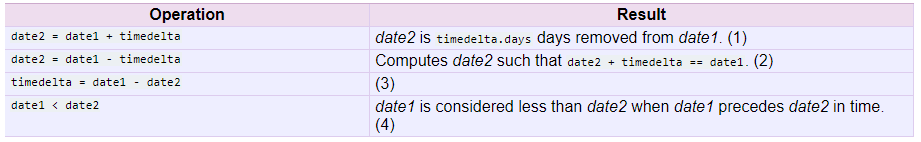
\includegraphics[width=0.90\textwidth]{figures/DateTime2}}
	\caption{Support Operation}
	\label{Support Opperation}
\end{figure}

\vspace{\baselineskip}
\noindent 
\begin{enumerate}
	\item Getting formatted time \par
\end{enumerate}
\noindent 
Anda dapat memformat kapan saja sesuai kebutuhan Anda, namun metode sederhana untuk mendapatkan waktu dalam format yang mudah dibaca adalah asctime () - \par
\noindent 
 \hspace*{0.5in}  $  \#  $!/usr/bin/python \par
\noindent 
 \hspace*{0.5in} import time; \par
\vspace{12pt}
\noindent 
 \hspace*{0.5in} localtime = time.asctime( time.localtime(time.time()) ) \par
\noindent 
 \hspace*{0.5in} print "Local current time :", localtime \par
\vspace{12pt}
\noindent 
Ini akan menghasilkan hasil sebagai berikut - \par
\noindent 
 \hspace*{0.5in} Local current time : Tue Jan 13 10:17:09 2009 \par
\vspace{12pt}
\vspace{12pt}
\noindent 
public static String getCurrentTimeStamp ()  $  \{  $ \par
\noindent 
 $  $ $  $ $  $ $  $ SimpleDateFormat sdfDate = new SimpleDateFormat ("yyyy-MM-dd HH: mm: ss"); // dd / MM / yyyy \par
\noindent 
 $  $ $  $ $  $ $  $ Tanggal sekarang = tanggal baru (); \par
\noindent 
 $  $ $  $ $  $ $  $ String strDate = sdfDate.format (sekarang); \par
\noindent 
 $  $ $  $ $  $ $  $ kembali strDate; \par
\noindent 
 $  \}  $ \par
\vspace{\baselineskip}
\noindent 
Saya mendapatkan tanggal dalam format 2009-09-22 16:47:08 (YYYY-MM-DD HH: MI: Sec). \par
\vspace{12pt}
\noindent 
Tapi saya ingin mengambil waktu sekarang dalam format 2009-09-22 16: 47: 08.128 ((YYYY-MM-DD HH: MI: Sec.Ms). \par
\vspace{12pt}
\noindent 
dimana 128 menceritakan milidetik. \par
\vspace{12pt}
\noindent 
SimpleTextFormat akan bekerja dengan baik. Di sini satuan waktu paling rendah adalah yang kedua, tapi bagaimana cara mendapatkan milidetik juga? \par
\noindent 
FYI, kelas tanggal tua yang merepotkan seperti java.util.Date, java.util.Calendar, dan java.text.SimpleTextFormat sekarang warisan, digantikan oleh kelas java.time. \par
\vspace{12pt}
\vspace{14pt}

\begin{itemize}
	\item Instance Attributes
\end{itemize}

\begin{figure}[ht]
	\centerline{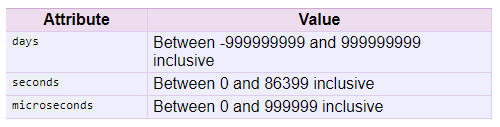
\includegraphics[width=0.90\textwidth]{figures/DateTime}}
	\caption{Instance Attributes}
	\label{Instance Attributes}
\end{figure}


\vspace{\baselineskip}
\noindent 
\begin{enumerate}
	\item Getting calendar for a month
\end{enumerate}
\noindent 
Modul kalender memberikan berbagai macam metode untuk dimainkan dengan kalender tahunan dan bulanan. Di sini, kami mencetak kalender untuk bulan tertentu (Jan 2008) - \par
\noindent 
 \hspace*{0.5in}  $  \#  $!/usr/bin/python \par
\noindent 
 \hspace*{0.5in} import calendar \par
\vspace{12pt}
\noindent 
 \hspace*{0.5in} cal = calendar.month(2008, 1) \par
\noindent 
 \hspace*{0.5in} print "Here is the calendar:" \par
\noindent 
 \hspace*{0.5in} print cal \par
\vspace{\baselineskip}
\noindent 
Ini akan menghasilkan hasil sebagai berikut - \par
\noindent 
 \hspace*{0.5in} Here is the calendar: \par
\noindent 
~~~  \hspace*{0.5in}  \hspace*{0.5in} January 2008 \par
\noindent 
 \hspace*{0.5in} Mo Tu We Th Fr Sa Su \par
\noindent 
~~~  \hspace*{0.5in}  \hspace*{0.5in} 1~ 2~~3~~4  5  6 \par
\noindent 
  \hspace*{0.5in}  \hspace*{0.5in} 7~ 8~ 9 10 11 12 13 \par
\noindent 
 \hspace*{0.5in}  \hspace*{0.5in} 14 15 16 17 18 19 20 \par
\noindent 
 \hspace*{0.5in}  \hspace*{0.5in} 21 22 23 24 25 26 27 \par
\noindent 
 \hspace*{0.5in}  \hspace*{0.5in} 28 29 30 31 \par
\noindent 

 \subsection {Android}
 \vspace{\baselineskip}
\noindent 
Pergi ke hari tertentu \par
\noindent 
Buka Google Kalender app Calendar. \par
\noindent 
Di kiri atas, ketuk nama bulan. Misalnya, January Down Arrow. \par
\noindent 
Gesek ke kiri atau kanan untuk pergi ke bulan lainnya. \par
\noindent 
Ketuk tanggal untuk melihat acara pada hari itu. \par
\noindent 
Kembali ke hari ini: Di pojok kanan atas, sentuh View today Event. \par
\vspace{12pt}
\noindent 
Pilih berapa hari untuk melihat \par
\noindent 
Saat membuka aplikasi Kalender, Anda akan melihat daftar acara mendatang Anda. Anda dapat mengalihkan pandangan untuk melihat keseluruhan hari atau beberapa hari Anda. \par
\vspace{12pt}
\noindent 
Buka Google Kalender app Calendar. \par
\noindent 
Di sudut kiri atas, tekan Menu Menu. \par
\noindent 
Pilih tampilan, seperti Jadwal atau Bulan. Untuk melihat semua acara, sasaran, dan pengingat Anda dalam daftar yang dipecah berdasarkan hari, pilih "Jadwal". \par
\noindent 

 \subsection {Computer}
\noindent 
Ubah tampilan kalender Anda \par
\noindent 
Ubah sementara \par
\noindent 
Tetapkan tampilan default baru \par
\noindent 
Arahkan kalender Anda \par
\noindent 
Ada dua cara untuk berpindah antar tanggal: \par
\vspace{12pt}
\noindent 
Gunakan tanda panah di pojok kiri atas Kalender untuk beralih ke tanggal terakhir di masa lalu atau masa depan. \par
\noindent 
Gunakan kalender kecil di pojok kiri atas untuk memilih tanggal. \par
\noindent 
Untuk kembali ke tanggal hari ini, klik Hari ini di pojok kiri atas. \par
\vspace{12pt}
\noindent 
Artikel terkait \par
\noindent 
Ubah pengaturan kalender Anda \par
\noindent 
Buat kalender baru \par


\noindent 
 \subsection { Iphone dan Ipad }
\noindent 
Pergi ke hari tertentu \par
\noindent 
Buka Google Kalender app Calendar. \par
\noindent 
Di kiri atas, ketuk nama bulan. Misalnya, January Down Arrow. \par
\noindent 
Gesek ke kiri atau kanan untuk pergi ke bulan lainnya. \par
\noindent 
Ketuk tanggal untuk melihat acara pada hari itu. \par
\noindent 
Kembali ke hari ini: Di pojok kanan atas, sentuh View today Event. \par
\vspace{12pt}
\noindent 
Pilih berapa hari untuk melihat \par
\noindent 
Saat membuka aplikasi Kalender, Anda akan melihat daftar acara mendatang Anda. Anda dapat mengalihkan pandangan untuk melihat keseluruhan hari atau beberapa hari Anda. \par
\vspace{12pt}
\noindent 
Buka Google Kalender app Calendar. \par
\noindent 
Di sudut kiri atas, tekan Menu Menu. \par
\noindent 
Pilih tampilan, seperti Jadwal atau Bulan. Untuk melihat semua acara, sasaran, dan pengingat Anda dalam daftar yang dipecah berdasarkan hari, pilih "Jadwal". \par
\noindent 
Ubah pengaturan Anda \par
\noindent 
Pelajari cara mengubah setelan kalender Anda, termasuk tampilan kalender dan hari dimulai. \par
\vspace{\baselineskip}
\noindent 
\begin{itemize}
\item The time Module
\end{itemize}
\noindent 
 \hspace*{0.5in} Ada modul waktu populer yang tersedia dengan Python yang menyediakan fungsi untuk bekerja dengan waktu dan untuk mengkonversi antara representasi. Berikut adalah daftar semua metode yang tersedia – \par
\noindent 
Modul ini menyediakan berbagai fungsi yang berkaitan dengan waktu. Untuk fungsionalitas terkait, lihat juga modul kalender dan kalender. \par
\vspace{12pt}
\noindent 
Meski modul ini selalu tersedia, tidak semua fungsi tersedia di semua platform. Sebagian besar fungsi yang didefinisikan dalam modul ini memanggil fungsi library C library dengan nama yang sama. Terkadang ada baiknya untuk berkonsultasi dengan dokumentasi platform, karena semantik fungsi ini bervariasi antar platform. \par
\noindent 
Penjelasan tentang beberapa terminologi dan konvensi adalah teratur. \par
\vspace{12pt}
\noindent 
Epoch adalah titik di mana waktu dimulai. Pada tanggal 1 Januari tahun itu, pada 0 jam, "waktu sejak zaman" adalah nol. Untuk Unix, eposnya adalah 1970. Untuk mengetahui apa zamannya, lihatlah gmtime (0). \par
\vspace{12pt}
\noindent 
Fungsi dalam modul ini tidak menangani tanggal dan waktu sebelum zaman atau jauh di masa depan. Titik potong di masa depan ditentukan oleh perpustakaan C; untuk Unix, biasanya pada tahun 2038. \par
\vspace{12pt}
\noindent 
Masalah tahun 2000 (Y2K): Python bergantung pada perpustakaan C platform, yang umumnya tidak memiliki masalah tahun 2000, karena semua tanggal dan waktu diwakili secara internal sebagai detik sejak zaman itu. Fungsi menerima struct $  \_  $time (lihat di bawah) umumnya memerlukan 4 digit tahun. Untuk kompatibilitas, 2 digit tahun didukung jika variabel modul accept2dyear adalah bilangan bulat nol nol; variabel ini diinisialisasi ke 1 kecuali variabel lingkungan PYTHONY2K diatur ke string yang tidak kosong, dalam hal ini diinisialisasi menjadi 0. Dengan demikian, Anda dapat mengatur PYTHONY2K ke string yang tidak kosong di lingkungan untuk meminta digit 4 digit untuk semua masukan tahun. Bila 2 digit tahun diterima, mereka dikonversi sesuai dengan standar POSIX atau X / Open: nilai 69-99 dipetakan ke 1969-1999, dan nilai 0-68 dipetakan ke 2000-2068. Nilai 100-1899 selalu ilegal. \par
\vspace{12pt}
\noindent 
UTC adalah Coordinated Universal Time (sebelumnya dikenal sebagai Greenwich Mean Time, atau GMT). Akronim UTC bukan kesalahan tapi kompromi antara bahasa Inggris dan Prancis. \par
\vspace{12pt}
\noindent 
DST adalah Daylight Saving Time, penyesuaian zona waktu dengan (biasanya) satu jam selama bagian tahun ini. Aturan DST adalah sihir (ditentukan oleh hukum setempat) dan bisa berubah dari tahun ke tahun. Perpustakaan C memiliki tabel yang berisi peraturan lokal (seringkali dibaca dari file sistem untuk fleksibilitas) dan merupakan satu-satunya sumber Kebijaksanaan Sejati dalam hal ini. \par
\vspace{12pt}
\noindent 
Ketepatan berbagai fungsi real-time mungkin kurang dari yang disarankan oleh unit di mana nilai atau argumen mereka diungkapkan. Misalnya. Pada sebagian besar sistem Unix, jam "kutu" hanya 50 atau 100 kali per detik. \par
\vspace{12pt}
\noindent 
Di sisi lain, ketepatan waktu () dan sleep () lebih baik daripada padanan Unix mereka: waktu dinyatakan sebagai bilangan floating point, waktu () mengembalikan waktu paling akurat yang tersedia (menggunakan Unix gettimeofday () jika tersedia), dan tidur () akan menerima waktu dengan pecahan tak-nol (Unix select () digunakan untuk menerapkan ini, jika tersedia). \par
\vspace{12pt}
\noindent 
Nilai waktu seperti yang dikembalikan oleh gmtime (), localtime (), dan strptime (), dan diterima oleh asctime (), mktime () dan strftime (), dapat dianggap sebagai urutan dari 9 bilangan bulat. Nilai kembalian gmtime (), localtime (), dan strptime () juga menawarkan nama atribut untuk masing-masing bidang. \par
\vspace{12pt}
\noindent 
Lihat struct $  \_  $time untuk deskripsi objek ini. \par
\vspace{12pt}
\noindent 
Berubah dalam versi 2.2: Urutan nilai waktu diubah dari tupel menjadi struct $  \_  $time, dengan penambahan nama atribut untuk field. \par
\vspace{\baselineskip}
\noindent 
\begin{itemize}
\item The calendar Module
\end{itemize}
\noindent 
Modul kalender memasok fungsi yang berhubungan dengan kalender, termasuk fungsi untuk mencetak kalender teks untuk bulan atau tahun tertentu. \par
\noindent 
Secara default, kalender mengambil hari Senin sebagai hari pertama minggu dan minggu sebagai yang terakhir. Untuk mengubah ini, fungsi call calendar.setfirstweekday (). \par
\noindent 
Berikut adalah daftar fungsi yang tersedia dengan modul kalender: \par
\noindent 
Modul ini memungkinkan Anda untuk menampilkan kalender seperti program cal Unix, dan menyediakan fungsi berguna tambahan yang terkait dengan kalender. Secara default, kalender ini Senin sebagai hari pertama dalam seminggu, dan hari minggu sebagai yang terakhir (konvensi Eropa). Gunakan setfirstweekday () untuk mengatur hari pertama dalam seminggu sampai Minggu (6) atau ke hari kerja lainnya. Parameter yang menentukan tanggal diberikan sebagai bilangan bulat. Untuk fungsionalitas terkait, lihat juga modul waktu dan waktu. \par
\vspace{12pt}
\noindent 
Sebagian besar fungsi dan kelas bergantung pada modul datetime yang menggunakan kalender ideal, kalender Gregorian saat ini tanpa batas diperpanjang di kedua arah. Ini sesuai dengan definisi kalender "pakar Gregorian" di buku Dershowitz dan Reingold "Perhitungan Calendrical", di mana kalender dasar untuk semua perhitungan. \par
\vspace{12pt}
\noindent 
kalender kelas.Calendar ([firstweekday]) \par
\noindent 
Membuat objek Kalender. Firstweekday adalah bilangan bulat yang menentukan hari pertama dalam seminggu. 0 adalah hari Senin (default), 6 adalah hari minggu. \par
\vspace{12pt}
\noindent 
Objek Kalender menyediakan beberapa metode yang dapat digunakan untuk menyiapkan data kalender untuk pemformatan. Kelas ini tidak melakukan format apapun itu sendiri. Ini adalah tugas dari subclass. \par
\vspace{12pt}
\noindent 
Baru di versi 2.5. \par
\vspace{12pt}
\noindent 
Contoh kalender memiliki metode berikut: \par
\vspace{12pt}
\noindent 
iterweekdays () \par
\noindent 
Kembalikan iterator untuk nomor hari minggu yang akan digunakan selama satu minggu. Nilai pertama dari iterator akan sama dengan nilai properti first weekekday. \par
\vspace{12pt}
\noindent 
ini bulan depan (tahun, bulan) \par
\noindent 
Kembalikan iterator untuk bulan bulan (1-12) di tahun tahun. Iterator ini akan mengembalikan semua hari (sebagai objek datetime.date) untuk bulan dan semua hari sebelum awal bulan atau setelah akhir bulan yang diperlukan untuk mendapatkan minggu yang lengkap. \par
\vspace{12pt}
\noindent 
itermonthdays2 (tahun, bulan) \par
\noindent 
Kembalikan iterator untuk bulan bulan di tahun yang sama dengan bulan tersebut (). Hari yang dikembalikan akan berupa tupel yang terdiri dari nomor hari dan nomor hari minggu. \par
\vspace{12pt}
\noindent 
itermonthdays (tahun, bulan) \par
\noindent 
Kembalikan iterator untuk bulan bulan di tahun yang sama dengan bulan tersebut (). Hari kembali hanya akan menjadi nomor hari. \par
\vspace{12pt}
\noindent 
monthdatescalendar (tahun, bulan) \par
\noindent 
Kembalikan daftar minggu di bulan bulan dalam setahun sebagai minggu penuh. Weeks adalah daftar tujuh objek datetime.date. \par
\vspace{12pt}
\noindent 
monthdays2calendar (tahun, bulan) \par
\noindent 
Kembalikan daftar minggu di bulan bulan dalam setahun sebagai minggu penuh. Weeks adalah daftar tujuh tupel nomor hari dan nomor hari kerja. \par
\vspace{12pt}
\noindent 
monthdayscalendar (tahun, bulan) \par
\noindent 
Kembalikan daftar minggu di bulan bulan dalam setahun sebagai minggu penuh. Weeks adalah daftar tujuh nomor hari. \par
\vspace{12pt}
\noindent 
yeardatescalendar (tahun [, lebar]) \par
\noindent 
Kembalikan data untuk tahun yang ditentukan untuk format. Nilai kembalian adalah daftar baris bulan. Setiap baris bulan berisi sampai berbulan-bulan (default ke 3). Setiap bulan mengandung antara 4 dan 6 minggu dan setiap minggu mengandung 1-7 hari. Hari adalah objek datetime.date. \par
\vspace{12pt}
\noindent 
yeardays2calendar (tahun [, lebar]) \par
\noindent 
Kembalikan data untuk tahun yang ditentukan untuk format (mirip dengan yeardatescalendar ()). Entri dalam daftar minggu adalah tupel nomor hari dan nomor hari kerja. Nomor hari di luar bulan ini adalah nol. \par
\vspace{12pt}
\noindent 
yeardayscalendar (tahun [, lebar]) \par
\noindent 
Kembalikan data untuk tahun yang ditentukan untuk format (mirip dengan yeardatescalendar ()). Entri dalam daftar minggu adalah nomor hari. Nomor hari di luar bulan ini adalah nol. \par
\vspace{12pt}
\noindent 
kalender kelas.TextCalendar ([firstweekday]) \par
\noindent 
Kelas ini bisa digunakan untuk menghasilkan teks biasa. \par
\vspace{12pt}
\noindent 
Baru di versi 2.5. \par
\vspace{12pt}
\noindent 
Contoh TextCalendar memiliki metode berikut: \par
\vspace{12pt}
\noindent 
format bulan (theyear, theyonth [, w [, l]]) \par
\noindent 
Kembalikan kalender bulan dalam string multi-baris. Jika w disediakan, kolom tersebut menentukan lebar kolom tanggal, yang dipusatkan. Jika saya diberi, itu menentukan jumlah baris yang akan digunakan setiap minggu. Tergantung pada hari kerja pertama seperti yang ditentukan dalam konstruktor atau ditetapkan oleh metode setfirstweekday (). \par
\vspace{12pt}
\noindent 
prmonth (theyear, theyonth [, w [, l]]) \par
\noindent 
Cetak kalender bulan yang dikembalikan menurut format bulan (). \par
\vspace{12pt}
\noindent 
formatyear (theyear [, w [, l [, c [, m]]]]) \par
\noindent 
Kembalikan kalender m-kolom selama satu tahun penuh sebagai string multi-baris. Parameter opsional w, l, dan c adalah untuk lebar kolom tanggal, garis per minggu, dan jumlah spasi di antara kolom bulan. Tergantung pada hari kerja pertama seperti yang ditentukan dalam konstruktor atau ditetapkan oleh metode setfirstweekday (). Tahun paling awal dimana kalender dapat dihasilkan bergantung pada platform. \par
\vspace{12pt}
\noindent 
pryear (theyear [, w [, l [, c [, m]]]]) \par
\noindent 
Cetak kalender selama satu tahun penuh seperti yang dikembalikan oleh formatyear (). \par
\vspace{12pt}
\noindent 
kalender kelas.HTMLCalendar ([firstweekday]) \par
\noindent 
Kelas ini bisa digunakan untuk membuat kalender HTML. \par
\vspace{12pt}
\noindent 
Baru di versi 2.5. \par
\vspace{12pt}
\noindent 
Contoh HTMLCalendar memiliki metode berikut: \par
\vspace{12pt}
\noindent 
formatmonth (theyear, theyonth [, withyear]) \par
\noindent 
Kembalikan kalender bulan sebagai tabel HTML. Jika tahun pertama benar tahun akan disertakan dalam header, jika tidak hanya nama bulan akan digunakan. \par
\vspace{12pt}
\noindent 
formatyear (theyear [, width]) \par
\noindent 
Kembalikan kalender satu tahun sebagai tabel HTML. lebar (default ke 3) menentukan jumlah bulan per baris. \par
\vspace{12pt}
\noindent 
formatyearpage (theyear [, width [, css [, encoding]]]) \par
\noindent 
Kembali a \par
\vspace{12pt}
\noindent 
\begin{itemize}
\item Other Modules\&Functions:
\end{itemize}
\noindent 
Jika Anda tertarik, maka di sini Anda akan menemukan daftar modul dan fungsi penting lainnya untuk bermain dengan tanggal  $  \&  $ waktu dengan Python: \par
\vspace{12pt}
\vspace{12pt}
\vspace{12pt}
\vspace{12pt}



\chapter{Dictionary}
\section{Python Dictionary}
Dictionary Python adalah kumpulan pasangan kunci:nilai (selanjutnya disebut: key-value) yang tak berurutan. Dictionary Python ini sama halnya dengan hash-table atau array-asosiatif di pemrograman Perl.

Suatu kunci (key) pada Dictionary bersifat Unique (unik), yang artinya adalah satu kunci hanya memiliki satu nilai. Aturan penulisannya berupa key:value. Sebuah Dictionary ditandai dengan adanya kurung kurawal “{}”. Setiap pasangan key:value dipisah dengan tanda koma. 

Setiap kunci dipisahkan dari nilainya oleh titik dua (:), item dipisahkan oleh koma, dan semuanya tertutup dalam kurung kurawal. Kamus kosong tanpa barang ditulis hanya dengan dua kurung kurawal, seperti ini:  \$  \{  \$ \$  \}  \$.

Kunci unik dalam kamus sementara nilai mungkin tidak. Nilai kamus bisa berupa tipe apa pun, namun kunci harus berupa tipe data yang tidak berubah seperti string, angka, atau tupel.

Dictionary menyediakan wadah yang sangat berguna yang memungkinkan kita mencari nilai menggunakan kunci\cite{oliphant2007python}. Dalam sebuah Dictionary tidak boleh ada dua key yang sama, maka memberikan nilai ke key yang sudah ada akan menghapus nilai yang lama. Untuk menambah key baru, Python memiliki syntax yang sama. Ini bisa menimbulkan kerancuan pada saat akan melakukan penambahan key baru, tapi ternyata hanya mengubah key yang sudah ada. Sebagai catatan, key yang baru terletak di bagian tengah bukan di belakang. Hal tersebut kebetulan saja, karena sebenarnya pada Dictionary memang tidak ada standar pengurutan yang berlaku.

\subsection{Accessing Values in Dictionary}
Untuk mengakses elemen kamus, Anda dapat menggunakan tanda kurung siku yang sudah dikenal bersama dengan kunci untuk mendapatkan nilainya. Berikut adalah contoh sederhana :
\begin{verbatim}  
  \$  \#  \$!/usr/bin/python
  dict =  \$  \{  \$'Name': 'Zara', 'Age': 7, 'Class': 'First' \$  \}  \$ 
 print "dict['Name']: ", dict['Name'] 
 print "dict['Age']: ", dict['Age']
\end{verbatim}
Bila kode diatas dieksekusi, maka menghasilkan hasil sebagai berikut :
dict['Name']:~ Zara
dict['Age']:~ 7 
Jika kita mencoba mengakses item data dengan sebuah kunci, yang bukan bagian dari kamus, kita mendapatkan error sebagai berikut :
\begin{verbatim} 
\$  \#  \$!/usr/bin/python
dict =  \$  \{  \$'Name': 'Zara', 'Age': 7, 'Class': 'First' \$  \}  \$ 
print "dict['Alice']: ", dict['Alice']
\end{verbatim}
Bila kode diatas dieksekusi, maka menghasilkan hasil sebagai berikut :
dict['Alice']: 
Traceback (most recent call last):
~~ File "test.py", line 4, in <module>
~~~~~  \print "dict['Alice']: ", dict['Alice']; 
KeyError: 'Alice' 

\subsection{Updating Dictionary}
Anda dapat memperbarui kamus dengan menambahkan entri baru atau pasangan nilai kunci, memodifikasi entri yang ada, atau menghapus entri yang ada seperti yang ditunjukkan di bawah ini dalam contoh sederhana :
\begin{verbatim}
\$  \#  \$!/usr/bin/python 
  dict =  \$  \{  \$'Name': 'Zara', 'Age': 7, 'Class': 'First' \$  \}  \$ 
  dict['Age'] = 8;  \$  \#  \$ update existing entry
  dict['School'] = "DPS School";  \$  \#  \$ Add new entry
  print "dict['Age']: ", dict['Age']
  print "dict['School']: ", dict['School']
\end{verbatim}
Bila kode diatas dieksekusi, maka menghasilkan hasil sebagai berikut : 
  dict['Age']:~ 8 
  dict['School']:~ DPS School 
  
\subsection{Delete Dictionary Elements}
Anda dapat menghapus elemen kamus individual atau menghapus keseluruhan isi kamus. Anda juga dapat menghapus seluruh kamus dalam satu operasi. 
Untuk menghapus seluruh kamus secara eksplisit, cukup gunakan del statement. Berikut adalah contoh sederhana : 
\begin{verbatim}   
   \$  \#  \$!/usr/bin/python
  dict =  \$  \{  \$'Name': 'Zara', 'Age': 7, 'Class': 'First' \$  \}  \$
  del dict['Name'];  \$  \#  \$ remove entry with key 'Name'
  dict.clear();~~~~  \$  \#  \$ remove all entries in dict 
  del dict~;~~~~~~   \$  \#  \$ delete entire dictionary 
  print "dict['Age']: ", dict['Age'] 
  print "dict['School']: ", dict['School']
\end{verbatim}  
Ini menghasilkan hasil berikut. Perhatikan bahwa pengecualian diajukan karena setelah kamus del dict tidak ada lagi - 
  dict['Age']: 
  Traceback (most recent call last): 
~   File "test.py", line 8, in <module> 
~~~     print "dict['Age']: ", dict['Age']; 
  TypeError: 'type' object is unsubscriptable 
Note: del () metode dibahas di bagian selanjutnya. 

\subsection{Properties of Dictionary Keys} 
Nilai kamus tidak memiliki batasan. Mereka bisa menjadi objek Python yang sewenang-wenang, baik objek standar atau objek yang ditentukan pengguna. Namun, hal yang sama tidak berlaku untuk kunci. 
Ada dua hal penting yang perlu diingat tentang kunci kamus – 
Lebih dari satu entri per kunci tidak diperbolehkan. Yang berarti tidak ada kunci duplikat yang diperbolehkan. Ketika kunci duplikat ditemui selama penugasan, tugas terakhir akan menang. Sebagai contoh – 
\begin{verbatim}   
   \$  \#  \$!/usr/bin/python 
  dict =  \$  \{  \$'Name': 'Zara', 'Age': 7, 'Name': 'Manni' \$  \}  \$ 
  print "dict['Name']: ", dict['Name']
\end{verbatim}  
Bila kode diatas dieksekusi, maka menghasilkan hasil sebagai berikut : 
  dict['Name']:~ Manni 
(b) Tombol harus tidak berubah. Yang berarti Anda bisa menggunakan string, angka atau tupel sebagai tombol kamus tapi sesuatu seperti ['key'] tidak diperbolehkan. Berikut adalah contoh sederhana: 
\begin{verbatim}   
   \$  \#  \$!/usr/bin/python 
  dict =  \$  \{  \$['Name']: 'Zara', 'Age': 7 \$  \}  \$ 
  print "dict['Name']: ", dict['Name']
\end{verbatim}
Bila kode diatas dieksekusi, maka menghasilkan hasil sebagai berikut : 
  Traceback (most recent call last): 
~~     File "test.py", line 3, in <module> 
~~~~~     dict =  \$  \{  \$['Name']: 'Zara', 'Age': 7 \$  \}  \$; 
  TypeError: list objects are unhashable 
Built-in Dictionary Functions  \$  \&  \$ Methods  \$ - \$ 
Python includes the following dictionary functions  \$ - \$ 
Python includes following dictionary methods  \$ - \$ 

\subsection{Dictionaries Introductions} 
Kami sudah mengenal daftar di bab sebelumnya. Di bab kusus Python online kami akan mempresentasikan kamus dan operator dan metode pada kamus. Program atau skrip Python tanpa daftar dan kamus hampir tidak dapat dibayangkan. Seperti daftar kamus yang bisa dengan mudah diubah, bisa menyusut dan berkembang ad libitum pada saat run time. Mereka menyusut dan tumbuh tanpa perlu membuat salinan. Kamus dapat dimuat dalam daftar dan sebaliknya. Tapi apa perbedaan antara daftar dan kamus? Daftar diurutkan dari objek, sedangkan kamus tidak berurutan. Tapi perbedaan utamanya adalah item dalam kamus diakses melalui kunci dan tidak melalui posisinya. Kamus adalah array asosiatif (juga dikenal sebagai hash). Kunci kamus mana pun dikaitkan (atau dipetakan) ke sebuah nilai. Nilai kamus bisa berupa tipe data Python. Jadi kamus adalah pasangan kunci-nilai tak berurutan. 
Kamus tidak mendukung urutan operasi dari jenis data urutan seperti string, tupel dan daftar. Kamus termasuk tipe pemetaan built-in. Mereka adalah satu-satunya wakil semacam ini! 
Di akhir bab ini, kami akan menunjukkan bagaimana kamus dapat diubah menjadi satu daftar, berisi (kunci, nilai) -tupel atau dua daftar, yaitu satu dengan kunci dan satu dengan nilainya. Transformasi ini bisa dilakukan secara terbalik juga. 

\subsection{How to create a dictionary?}
Membuat kamus sama mudahnya dengan menempatkan item dalam kurung kurawal  \$  \{  \$ \$  \}  \$ dipisahkan dengan koma. Item memiliki kunci dan nilai yang sesuai dinyatakan sebagai pasangan, kunci: nilai. Sementara nilai dapat berupa tipe data apa pun dan dapat diulang, kunci harus terdiri dari tipe yang tidak dapat diubah (string, number atau tupel dengan elemen yang tidak berubah) dan harus unik. 
\begin{verbatim}
   \$  \#  \$ empty dictionary 
  my \$  \_  \$dict =  \$  \{  \$ \$  \}  \$ 
   \$  \#  \$ dictionary with integer keys 
  my \$  \_  \$dict =  \$  \{  \$1: 'apple', 2: 'ball' \$  \}  \$ 
   \$  \#  \$ dictionary with mixed keys 
  my \$  \_  \$dict =  \$  \{  \$'name': 'John', 1: [2, 4, 3] \$  \}  \$ 
   \$  \#  \$ using dict() 
  my \$  \_  \$dict = dict( \$  \{  \$1:'apple', 2:'ball' \$  \}  \$) 
   \$  \#  \$ from sequence having each item as a pair 
  my \$  \_  \$dict = dict([(1,'apple'), (2,'ball')])
\end{verbatim}
Seperti yang bisa Anda lihat di atas, kita juga bisa membuat kamus menggunakan fungsi built-in dict (). 

\subsection{How to access elements from a dictionary?} 
Sementara pengindeksan digunakan dengan jenis wadah lain untuk mengakses nilai, kamus menggunakan tombol. Kunci dapat digunakan baik di dalam tanda kurung siku atau dengan metode get (). Perbedaan saat menggunakan get () adalah mengembalikan Elemen alih-alih KeyError, jika kuncinya tidak ditemukan. 
\begin{verbatim}
  my \$  \_  \$dict =  \$  \{  \$'name':'Jack', 'age': 26 \$  \}  \$ 
   \$  \#  \$ Output: Jack 
  print(my \$  \_  \$dict['name']) 
   \$  \#  \$ Output: 26 
  print(my \$  \_  \$dict.get('age')) 
   \$  \#  \$ Trying to access keys which doesn't exist throws error 
   \$  \#  \$ my \$  \_  \$dict.get('address') 
   \$  \#  \$ my \$  \_  \$dict['address'] 
\end{verbatim}   
Saat menjalankan program, hasilnya adalah: 
Jack 
26 

\subsection{How to change or add elements in a dictionary?}
Kamus bisa berubah-ubah. Kita bisa menambahkan item baru atau mengubah nilai barang yang ada menggunakan operator penugasan. 
Jika kuncinya sudah ada, nilai akan diperbarui, jika ada kunci baru: pasangan nilai ditambahkan ke kamus. 
Script.py
\begin{verbatim}
  my \$  \_  \$dict =  \$  \{  \$'name':'Jack', 'age': 26 \$  \}  \$ 
   \$  \#  \$ update value 
  my \$  \_  \$dict['age'] = 27 
   \$  \#  \$Output:  \$  \{  \$'age': 27, 'name': 'Jack' \$  \}  \$ 
  print(my \$  \_  \$dict) 
   \$  \#  \$ add item 
  my \$  \_  \$dict['address']~= 'Downtown'   
   \$  \#  \$ Output:  \$  \{  \$'address': 'Downtown', 'age': 27, 'name': 'Jack' \$  \}  \$ 
  print(my \$  \_  \$dict). 
\end{verbatim}  
Saat menjalankan program, hasilnya adalah: 

 \$  \{  \$'name': 'Jack', 'age': 27 \$  \}  \$ 
 \$  \{  \$'name': 'Jack', 'age': 27, 'address': 'Downtown' \$  \}  \$ 
 
\subsection{How to delete or remove elements from a dictionary?}
Kita bisa menghapus item tertentu dalam kamus dengan menggunakan metode pop (). Metode ini menghilangkan item dengan tombol yang disediakan dan mengembalikan nilainya. 
Metodenya, popitem () dapat digunakan untuk menghapus dan mengembalikan item yang sewenang-wenang (key, value) membentuk kamus. Semua item dapat dihapus sekaligus dengan menggunakan metode clear (). 
Kita juga bisa menggunakan kata kunci del untuk menghapus setiap item atau keseluruhan kamus itu sendiri. 
Scrip.py
\begin{verbatim}
   \$  \#  \$ create a dictionary 
  squares~=  \$  \{  \$1:1, 2:4, 3:9, 4:16, 5:25 \$  \}  \$   
   \$  \#  \$ remove a particular item 
   \$  \#  \$ Output: 16 
  print(squares.pop(4))~  
   \$  \#  \$ Output:  \$  \{  \$1: 1, 2: 4, 3: 9, 5: 25 \$  \}  \$ 
  print(squares) 
   \$  \#  \$ remove an arbitrary item 
   \$  \#  \$ Output: (1, 1) 
  print(squares.popitem()) 
   \$  \#  \$ Output:  \$  \{  \$2: 4, 3: 9, 5: 25 \$  \}  \$ 
  print(squares) 
   \$  \#  \$ delete a particular item 
  del~squares[5]   
   \$  \#  \$ Output:  \$  \{  \$2: 4, 3: 9 \$  \}  \$ 
  print(squares) 
   \$  \#  \$ remove all items 
  squares.clear() 
   \$  \#  \$ Output:  \$  \{  \$ \$  \}  \$ 
  print(squares) 
   \$  \#  \$ delete the dictionary itself 
  del squares 
  \$  \#  \$ Throws Error 
  \$  \#  \$ print(squares)
\end{verbatim}  
When you run the program, the output will be: 
16 
 \$  \{  \$1: 1, 2: 4, 3: 9, 5: 25 \$  \}  \$ 
(1, 1) 
 \$  \{  \$2: 4, 3: 9, 5: 25 \$  \}  \$ 
 \$  \{  \$2: 4, 3: 9 \$  \}  \$ 
 \$  \{  \$ \$  \}  \$ 
Tipe data daftar memiliki beberapa metode lagi. Berikut adalah semua metode daftar objek: 
list.append (x) 
Tambahkan item ke bagian akhir daftar; setara dengan [len (a):] = [x]. 
list.extend (L) 
Perluas daftar dengan menambahkan semua item dalam daftar yang diberikan; setara dengan [len (a):] = L. 
list.insert (i, x) 
Masukkan item pada posisi tertentu. Argumen pertama adalah indeks dari elemen yang sebelum dimasukkan, jadi a.insert (0, x) memasukkan di bagian depan daftar, dan a.insert (len (a), x) setara dengan a.append ( x). 
list.remove (x) 
Hapus item pertama dari daftar yang nilainya x. Ini adalah kesalahan jika tidak ada item seperti itu. 
list.pop ([i]) 
Hapus item pada posisi yang diberikan dalam daftar, dan kembalikan. Jika tidak ada indeks yang ditentukan, a.pop () menghapus dan mengembalikan item terakhir dalam daftar. (Tanda kurung siku di sekitar i pada tanda tangan metode menunjukkan bahwa parameternya adalah opsional, bukankah Anda harus mengetikkan tanda kurung siku pada posisi itu. Anda akan sering melihat notasi ini di Referensi Perpustakaan Python.) 
list.index (x) 
Kembalikan indeks di daftar item pertama yang nilainya x. Ini adalah kesalahan jika tidak ada item seperti itu. 
list.count (x) 
Kembalikan berapa kali x muncul dalam daftar. 
list.sort (cmp = None, key = None, reverse = False) 
Urutkan item daftar di tempat (argumen dapat digunakan untuk kustomisasi sortir, lihat diurutkan () untuk penjelasan mereka). 
list.reverse () 
Membalik unsur daftar, di tempat. 
Nilai Dictionary tidak memiliki batasan. Mereka bisa menjadi objek Python yang sewenang-wenang, baik objek standar atau objek yang ditentukan pengguna. Namun, hal yang sama tidak berlaku untuk key. 
Ada dua hal penting yang harus diingat tentang Dictionary Key. 
Pertama lebih dari satu entri per key tidak diperbolehkan. Yang berarti tidak ada key duplikat yang diperbolehkan. Saat key duplikat ditemui selama penugasan, tugas terakhir akan menang. 
Kedua key harus tidak berubah. Yang berarti Anda bisa menggunakan string, angka atau tuples sebagai tombol kamus tapi sesuatu seperti ['key'] tidak diperbolehkan. 


\chapter{Functions}
\section{Python Functions}\par
Fungsi adalah blok kode terorganisir dan dapat digunakan kembali yang digunakan untuk melakukan tindakan tunggal dan terkait. Fungsi menyediakan modularitas yang lebih baik untuk aplikasi Anda dan tingkat penggunaan kode yang tinggi. Seperti yang sudah Anda ketahui, Python memberi Anda banyak fungsi built-in seperti cetak (), dll. Tetapi Anda juga dapat membuat fungsi Anda sendiri. Fungsi ini disebut fungsi yang ditentukan pengguna. \par

function di Python biasanya mempunyai sebuah parameter dan return statement. Function di Python mempunyai pola sebagai berikut:
\begin{verbatim}
def nama function yang ingin anda buat (param1, param2, ... paramn):
   
   # kode Anda diisi
    return sesuatu
\end{verbatim}    
Tipe data yang dikembalikan bisa bermacam jenis tipe data yang didukung Python. Meskipun parameter yang akan diterima oleh function tersebut. 

\subsection{Defining a Function} \par
 Anda dapat menentukan fungsi untuk menyediakan fungsionalitas yang dibutuhkan. Berikut adalah aturan sederhana untuk mendefinisikan fungsi dengan Python. \par
\noindent 
 $ \bullet $ Blok fungsi dimulai dengan defensi kata kunci diikuti oleh nama fungsi dan tanda kurung (()). \par
\noindent 
 $ \bullet $ Setiap parameter masukan atau argumen harus ditempatkan di dalam tanda kurung ini. Anda juga dapat menentukan parameter di dalam tanda kurung ini. \par
\noindent 
 $ \bullet $ Pernyataan fungsi pertama dapat berupa pernyataan opsional - string dokumentasi fungsi atau docstring. \par
\noindent 
 $ \bullet $ Blok kode dalam setiap fungsi dimulai dengan titik dua (:) dan indentasi. \par
\noindent 
 $ \bullet $ Pernyataan kembali [ekspresi] keluar dari sebuah fungsi, secara opsional menyampaikan kembali ekspresi ke pemanggil. Pernyataan pengembalian tanpa argumen sama dengan return None. \par
\vspace{12pt}
\noindent 

\subsection{Syntax} \par
Berikut adalah contoh program kalkulator menggunakan Function pada Python : \par
\begin{verbatim}
def menu()
    print "Hallo Guys :) Selamat Datang di Program Kalkulator"
    print "Pilih Operasi Bilangan :"
    print " "
    print "1) Penjumlahan"
    print "2) Pengurangan"
    print "3) Perkalian"
    print "4) Pembagian"
    print "5) Keluar Program"
    print " "
    return input ("Pilih Operasi Matematikanya : ")

# Function untuk Penjumlahan
def tbh(a,b):
    print a, "+", b, "=", a + b

# Function untuk Pengurangan
def kur(a,b):
    print b, "+", a, "=", b + a

# Function untuk Perkalian
def kal(a,b):
    print a, "*", b, "=", a * b

# Function untuk Pembagian
def bag(a,b):
    print a, "/", b, "=", a / b

loop = 1
choice = 0
while loop == 1:
    choice = menu()
    if choice == 1:
        tbh(input("Tambahkan Ini: "),input("Dengan ini: "))
    elif choice == 2:
        kur(input("Kurangkan Ini: "),input("Dengan ini: "))
    elif choice == 3:
        kur(input("Kalikan Ini: "),input("Dengan ini: "))
    elif choice == 4:
        kur(input("Bagikan Ini: "),input("Dengan ini: "))
    elif choice == 5:
        loop = 0

print "GoodBye :( Terimakasih Telah Menggunakan calc.py :)"
\end{verbatim}

Berikut contoh Program Mencetak Menu dan Menghitung Luas menggunakan Function pada Python : \par
\begin{verbatim}
def menu(): 
print "Menu Options" 
print 
print "1. Segitiga" 
print "2. Persegi Panjang" 
print "3. Lingkaran" 
print "4. Keluar" 

def segitiga(): 
print "Menghitung Luas Segitiga" 
a = input("Tambahkan Alas : ") 
t = input("Tambahkan Tinggi : ") 
luas = (a*t)/2 
print "Luas Segitiga yaitu ",luas 
print 
print "Coba lagi [Y/N]? " 
back = raw_input().upper() 
if back == "Y": 
menu() 
else: 
exit()

def persegipanjang(): 
print "Menghitung Luas Persegi Panjang" 
p = input("Masukkan Panjang : ") 
l = input("Masukkan Lebar : ") 
luas = p*l 
print "Luas Persegi Panjang yaitu ",luas 
print 
print "Coba lagi [Y/N]? " 
back = raw_input().upper() 
if back == "Y": 
menu() 
else: 
exit() 

def lingkaran(): 
print "Menghitung Luas Lingkaran" 
r = input("Tambahkan Jari-Jari : ") 
luas = 3.14*(r**2) 
print "Luas Lingkaran yaitu ",luas 
print 
print "Coba lagi [Y/N]? " 
back = raw_input().upper() 
if back == "Y": 
menu() 
else: 
exit() 

#Program Perhitungan Luas 
print "Selamat Bahagia di Program Menghitung Luas" 
print "-----------------------------------------------" 
print 
menu() 
while l: 
#input 
pilih = input("Masukkan options : ") 
if pilih == 1: 
Segitiga() 
elif pilih == 2: 
Persegi Panjang() 
elif pilih == 3: 
Lingkaran() 
elif pilih == 4: 
print "\n"*100 
break 
else: 
print "Sorry Option yang di masukkan tidak ada" 
print "Coba lagi [Y/N] ? " 
coba = raw_input().upper() 
if coba == "Y": 
menu() 
else: 
print "\n"*100 
break
\end{verbatim}

\subsection{Parameter Fungsi} \par
Parameter Fungsi adalah sebuah fungsi yang dapat mempunyai daftar argumen (parameter) atau tidak. \par

\subsubsection{Parameter Posisi} \par
Parameter Posisi merupakan parameter fungsi pada urutan posisi yang valid. Saat pemanggilan fungsi, parameter itu diharuskan sesuai dengan jumlah parameter yang sudah didefinisikan. \par

Contoh : \par
\begin{verbatim}
def perhitunan (k,l) :
            m=k+l
            return m
perhitungan (4,5)
0utput = 9
\end{verbatim}

\noindent 
 \hspace*{0.5in} def functionname( parameters ): \par
\noindent 
~~  \hspace*{0.5in}  \hspace*{0.5in} "function $  \_  $docstring" \par
\noindent 
~~  \hspace*{0.5in}  \hspace*{0.5in} function $  \_  $suite \par
\noindent 
~~  \hspace*{0.5in}  \hspace*{0.5in} return [expression] \par
\noindent 
Secara default, parameter memiliki perilaku posisi dan Anda perlu memberi tahu mereka dengan urutan yang sama seperti yang ditetapkan. \par
\vspace{12pt}
\noindent 
Example \par
\noindent 
Fungsi berikut mengambil string sebagai parameter masukan dan mencetaknya di layar standar. \par
\noindent 
 \hspace*{0.5in} def printme( str ): \par
\noindent 
~~  \hspace*{0.5in}  \hspace*{0.5in} "This prints a passed string into this function" \par
\noindent 
~~  \hspace*{0.5in}  \hspace*{0.5in} print str \par
\noindent 
~~  \hspace*{0.5in}  \hspace*{0.5in} return \par
\vspace{12pt}
\noindent 
Calling a Function \par
\noindent 
Mendefinisikan sebuah fungsi hanya memberinya sebuah nama, menentukan parameter yang akan disertakan dalam fungsi dan menyusun blok kode. Setelah struktur dasar fungsi selesai, Anda dapat menjalankannya dengan memanggilnya dari fungsi lain atau langsung dari prompt Python. Berikut adalah contoh untuk memanggil fungsi printme () - \par
\noindent 
 \hspace*{0.5in}  $  \#  $!/usr/bin/python \par
\vspace{12pt}
\noindent 
 \hspace*{0.5in}  $  \#  $ Function definition is here \par
\noindent 
 \hspace*{0.5in} def printme( str ): \par
\noindent 
~~  \hspace*{0.5in}  \hspace*{0.5in} "This prints a passed string into this function" \par
\noindent 
~~  \hspace*{0.5in} print str \par
\noindent 
~~  \hspace*{0.5in} return; \par
\vspace{12pt}
\noindent 
 \hspace*{0.5in}  $  \#  $ Now you can call printme function \par
\noindent 
 \hspace*{0.5in} printme("I'm first call to user defined function!") \par
\noindent 
 \hspace*{0.5in} printme("Again second call to the same function") \par
\noindent 
Bila kode diatas dieksekusi, maka menghasilkan hasil sebagai berikut - \par
\noindent 
 \hspace*{0.5in} I'm first call to user defined function! \par
\noindent 
 \hspace*{0.5in} Again second call to the same function \par
\vspace{12pt}
\noindent 
Pass by reference vs value \par
\noindent 
Semua parameter (argumen) dalam bahasa Python dilewatkan dengan referensi. Ini berarti jika Anda mengubah parameter yang mengacu pada suatu fungsi, perubahan tersebut juga mencerminkan kembali fungsi pemanggilan. Sebagai contoh - \par
\noindent 
 \hspace*{0.5in}  $  \#  $!/usr/bin/python \par
\vspace{12pt}
\noindent 
 \hspace*{0.5in}  $  \#  $ Function definition is here \par
\noindent 
 \hspace*{0.5in} def changeme( mylist ): \par
\noindent 
 \hspace*{0.5in} ~~ "This changes a passed list into this function" \par
\noindent 
~~  \hspace*{0.5in}  \hspace*{0.5in} mylist.append([1,2,3,4]); \par
\noindent 
~~  \hspace*{0.5in} print "Values inside the function: ", mylist \par
\noindent 
~~  \hspace*{0.5in} return \par
\noindent 
 \hspace*{0.5in} \vspace{12pt}
\noindent 
 \hspace*{0.5in}  $  \#  $ Now you can call changeme function \par
\noindent 
 \hspace*{0.5in} mylist = [10,20,30]; \par
\noindent 
 \hspace*{0.5in} changeme( mylist ); \par
\noindent 
 \hspace*{0.5in} print "Values outside the function: ", mylist \par
\noindent 
Di sini, kita mempertahankan referensi objek yang dilewati dan menambahkan nilai pada objek yang sama. Jadi, ini akan menghasilkan hasil sebagai berikut - \par
\noindent 
 \hspace*{0.5in} Values~inside the function:  [10, 20, 30, [1, 2, 3, 4]] \par
\noindent 
 \hspace*{0.5in} Values~outside the function:  [10, 20, 30, [1, 2, 3, 4]] \par
\noindent 
Ada satu contoh lagi di mana argumen dilewatkan melalui referensi dan rujukannya ditimpa di dalam fungsi yang disebut. \par
\noindent 
 \hspace*{0.5in}  $  \#  $!/usr/bin/python \par
\vspace{12pt}
\noindent 
 \hspace*{0.5in}  $  \#  $ Function definition is here \par
\noindent 
 \hspace*{0.5in} def changeme( mylist ): \par
\noindent 
 \hspace*{0.5in} ~~ "This changes a passed list into this function" \par
\noindent 
 \hspace*{0.5in} ~~ mylist = [1,2,3,4];  $  \#  $ This would assig new reference in mylist \par
\noindent 
 \hspace*{0.5in} ~~ print "Values inside the function: ", mylist \par
\noindent 
 \hspace*{0.5in} ~~ return \par
\vspace{12pt}
\noindent 
 \hspace*{0.5in}  $  \#  $ Now you can call changeme function \par
\noindent 
 \hspace*{0.5in} mylist = [10,20,30]; \par
\noindent 
 \hspace*{0.5in} changeme( mylist ); \par
\noindent 
 \hspace*{0.5in} print "Values outside the function: ", mylist \par
\noindent 
Parameter mylist adalah local ke fungsi changeme. Mengubah mylist dalam fungsi tidak mempengaruhi mylist. Fungsi ini tidak menghasilkan apa-apa dan akhirnya ini akan menghasilkan hasil sebagai berikut: \par
\noindent 
 \hspace*{0.5in} Values~inside the function:  [1, 2, 3, 4] \par
\noindent 
 \hspace*{0.5in} Values~outside the function:  [10, 20, 30] \par
\vspace{12pt}
\noindent 
Function Arguments \par
\noindent 
Anda dapat memanggil fungsi dengan menggunakan jenis argumen formal berikut: \par
\noindent 
 \hspace*{0.5in}  $ \bullet $ Argumen yang dibutuhkan \par
\noindent 
 \hspace*{0.5in}  $ \bullet $ Argumen kata kunci \par
\noindent 
 \hspace*{0.5in}  $ \bullet $ Argumen baku \par
\noindent 
 \hspace*{0.5in}  $ \bullet $ Argumen panjang variable \par
\vspace{12pt}
\noindent 
Required arguments \par
\noindent 
Argumen yang diperlukan adalah argumen yang diberikan ke sebuah fungsi dalam urutan posisi yang benar. Di sini, jumlah argumen dalam pemanggilan fungsi harus sesuai persis dengan definisi fungsi. Untuk memanggil fungsi printme (), Anda pasti perlu melewati satu argumen, jika tidak maka akan memberikan kesalahan sintaks sebagai berikut - \par
\noindent 
 \hspace*{0.5in}  $  \#  $!/usr/bin/python \par
\vspace{12pt}
\noindent 
 \hspace*{0.5in}  $  \#  $ Function definition is here \par
\noindent 
 \hspace*{0.5in} def printme( str ): \par
\noindent 
~~  \hspace*{0.5in}  \hspace*{0.5in} "This prints a passed string into this function" \par
\noindent 
~~  \hspace*{0.5in} print str \par
\noindent 
~~  \hspace*{0.5in} return; \par
\vspace{12pt}
\noindent 
 \hspace*{0.5in}  $  \#  $ Now you can call printme function \par
\noindent 
 \hspace*{0.5in} printme() \par
\noindent 
Bila kode diatas dieksekusi, maka menghasilkan hasil sebagai berikut: \par
\noindent 
 \hspace*{0.5in} Traceback (most recent call last): \par
\noindent 
 \hspace*{0.5in} ~ File "test.py", line 11, in <module> \par
\noindent 
 \hspace*{0.5in} ~~~ printme(); \par
\noindent 
 \hspace*{0.5in} TypeError: printme() takes exactly 1 argument (0 given) \par
\vspace{12pt}
\noindent 
Keyword arguments \par
\noindent 
Argumen kata kunci terkait dengan pemanggilan fungsi. Bila Anda menggunakan argumen kata kunci dalam pemanggilan fungsi, penelepon mengidentifikasi argumen berdasarkan nama parameter. Hal ini memungkinkan Anda melewatkan argumen atau menempatkannya agar tidak bermasalah karena penerjemah Python dapat menggunakan kata kunci yang diberikan agar sesuai dengan nilai parameter. Anda juga dapat membuat panggilan kata kunci ke fungsi printme () dengan cara berikut - \par
\noindent 
 \hspace*{0.5in}  $  \#  $!/usr/bin/python \par
\vspace{12pt}
\noindent 
 \hspace*{0.5in}  $  \#  $ Function definition is here \par
\noindent 
 \hspace*{0.5in} def printme( str ): \par
\noindent 
 \hspace*{0.5in} ~~ "This prints a passed string into this function" \par
\noindent 
 \hspace*{0.5in} ~~ print str \par
\noindent 
 \hspace*{0.5in} ~~ return; \par
\vspace{12pt}
\noindent 
 \hspace*{0.5in}  $  \#  $ Now you can call printme function \par
\noindent 
 \hspace*{0.5in} printme( str = "My string") \par
\noindent 
Bila kode diatas dieksekusi, maka menghasilkan hasil sebagai berikut - \par
\noindent 
 \hspace*{0.5in} My string \par
\noindent 
Contoh berikut memberikan gambaran yang lebih jelas. Perhatikan bahwa urutan parameter tidak masalah. \par
\noindent 
 \hspace*{0.5in}  $  \#  $!/usr/bin/python \par
\vspace{12pt}
\noindent 
 \hspace*{0.5in}  $  \#  $ Function definition is here \par
\noindent 
 \hspace*{0.5in} def printinfo( name, age ): \par
\noindent 
 \hspace*{0.5in} ~~ "This prints a passed info into this function" \par
\noindent 
 \hspace*{0.5in} ~~ print "Name: ", name \par
\noindent 
 \hspace*{0.5in} ~~ print "Age ", age \par
\noindent 
 \hspace*{0.5in} ~~ return; \par
\vspace{12pt}
\noindent 
 \hspace*{0.5in}  $  \#  $ Now you can call printinfo function \par
\noindent 
 \hspace*{0.5in} printinfo( age=50, name="miki" ) \par
\noindent 
Bila kode diatas dieksekusi, maka menghasilkan hasil sebagai berikut - \par
\noindent 
 \hspace*{0.5in} Name:~ miki \par
\noindent 
 \hspace*{0.5in} Age~ 50 \par
\vspace{12pt}
\noindent 
Default arguments \par
\noindent 
Argumen default adalah argumen yang mengasumsikan nilai default jika nilai tidak diberikan dalam pemanggilan fungsi untuk argumen itu. Contoh berikut memberi ide pada argumen default, ini mencetak usia default jika tidak lulus - \par
\noindent 
 \hspace*{0.5in}  $  \#  $!/usr/bin/python \par
\vspace{12pt}
\noindent 
 \hspace*{0.5in}  $  \#  $ Function definition is here \par
\noindent 
 \hspace*{0.5in} def printinfo( name, age = 35 ): \par
\noindent 
 \hspace*{0.5in} ~~ "This prints a passed info into this function" \par
\noindent 
 \hspace*{0.5in} ~~ print "Name: ", name \par
\noindent 
 \hspace*{0.5in} ~~ print "Age ", age \par
\noindent 
 \hspace*{0.5in} ~~ return; \par
\vspace{12pt}
\noindent 
 \hspace*{0.5in}  $  \#  $ Now you can call printinfo function \par
\noindent 
 \hspace*{0.5in} printinfo( age=50, name="miki" ) \par
\noindent 
 \hspace*{0.5in} printinfo( name="miki" ) \par
\noindent 
Bila kode diatas dieksekusi, maka menghasilkan hasil sebagai berikut - \par
\noindent 
 \hspace*{0.5in} Name:~ miki \par
\noindent 
 \hspace*{0.5in} Age~ 50 \par
\noindent 
 \hspace*{0.5in} Name:~ miki \par
\noindent 
 \hspace*{0.5in} Age~ 35 \par
\vspace{12pt}
\noindent 
Variable-length arguments \par
\noindent 
Anda mungkin perlu memproses sebuah fungsi untuk argumen lebih banyak daripada yang Anda tentukan saat menentukan fungsinya. Argumen ini disebut variable-lengtharguments dan tidak disebutkan dalam definisi fungsi, tidak seperti argumen yang dibutuhkan dan standar. \par
\noindent 
Sintaks untuk fungsi dengan argumen variabel non-kata kunci adalah ini - \par
\noindent 
 \hspace*{0.5in} def functionname([formal $  \_  $args,] *var $  \_  $args $  \_  $tuple ): \par
\noindent 
 \hspace*{0.5in} ~~ "function $  \_  $docstring" \par
\noindent 
 \hspace*{0.5in} ~~ function $  \_  $suite \par
\noindent 
 \hspace*{0.5in} ~~ return [expression] \par
\noindent 
Tanda asterisk (*) ditempatkan sebelum nama variabel yang menyimpan nilai dari semua argumen variabel nonkeyword. Tuple ini tetap kosong jika tidak ada argumen tambahan yang ditentukan selama pemanggilan fungsi. Berikut adalah contoh sederhana - \par
\noindent 
 \hspace*{0.5in}  $  \#  $!/usr/bin/python \par
\vspace{12pt}
\noindent 
 \hspace*{0.5in}  $  \#  $ Function definition is here \par
\noindent 
 \hspace*{0.5in} def printinfo( arg1, *vartuple ): \par
\noindent 
 \hspace*{0.5in} ~~ "This prints a variable passed arguments" \par
\noindent 
 \hspace*{0.5in} ~~ print "Output is: " \par
\noindent 
 \hspace*{0.5in} ~~ print arg1 \par
\noindent 
 \hspace*{0.5in} ~~ for var in vartuple: \par
\noindent 
 \hspace*{0.5in} ~~~~~ print var \par
\noindent 
 \hspace*{0.5in} ~~ return; \par
\noindent 
 \hspace*{0.5in} \vspace{12pt}
\noindent 
 \hspace*{0.5in}  $  \#  $ Now you can call printinfo function \par
\noindent 
 \hspace*{0.5in} printinfo( 10 ) \par
\noindent 
 \hspace*{0.5in} printinfo( 70, 60, 50 ) \par
\noindent 
Bila kode diatas dieksekusi, maka menghasilkan hasil sebagai berikut - \par
\noindent 
 \hspace*{0.5in} Output is: \par
\noindent 
 \hspace*{0.5in} 10 \par
\noindent 
 \hspace*{0.5in} Output is: \par
\noindent 
 \hspace*{0.5in} 70 \par
\noindent 
 \hspace*{0.5in} 60 \par
\noindent 
 \hspace*{0.5in} 50 \par
\noindent 
The $  $Anonymous $  $Functions \par
\noindent 
Fungsi ini disebut anonim karena tidak dinyatakan secara standar dengan menggunakan kata kunci def. Anda bisa menggunakan kata kunci lambda untuk membuat fungsi anonim yang kecil. \par
\noindent 
 \hspace*{0.5in}  $ \bullet $ Bentuk lambda bisa mengambil sejumlah argumen tapi hanya mengembalikan satu nilai  \hspace*{0.5in} ~~ dalam bentuk ekspresi. Mereka tidak dapat berisi perintah atau beberapa ekspresi. \par
\noindent 
 \hspace*{0.5in}  $ \bullet $ Fungsi anonim tidak bisa menjadi panggilan langsung untuk dicetak karena lambda  \hspace*{0.5in} ~~ membutuhkan ekspresi \par
\noindent 
 \hspace*{0.5in}  $ \bullet $ Fungsi Lambda memiliki namespace lokal mereka sendiri dan tidak dapat mengakses  \hspace*{0.5in} ~ variabel selain yang ada dalam daftar parameter dan yang ada di namespace global. \par
\noindent 
 \hspace*{0.5in}  $ \bullet $ Meskipun tampak bahwa lambda adalah versi satu baris dari sebuah fungsi, mereka tidak  \hspace*{0.5in} ~ setara dengan pernyataan inline di C atau C ++, yang tujuannya adalah dengan  \hspace*{0.5in} ~~~~~~~ melewatkan alokasi stack fungsi selama pemanggilan untuk alasan kinerja. \par
\vspace{12pt}
\noindent 
Syntax \par
\noindent 
Sintaks fungsi lambda hanya berisi satu pernyataan, yaitu sebagai berikut - \par
\noindent 
 \hspace*{0.5in} lambda [arg1 [,arg2,.....argn]]:expression \par
\noindent 
Berikut adalah contoh untuk menunjukkan bagaimana lambda bentuk fungsi bekerja - \par
\noindent 
 \hspace*{0.5in}  $  \#  $!/usr/bin/python \par
\vspace{12pt}
\noindent 
 \hspace*{0.5in}  $  \#  $ Function definition is here \par
\noindent 
 \hspace*{0.5in} sum = lambda arg1, arg2: arg1 + arg2; \par
\vspace{12pt}
\noindent 
  \par
\vspace{12pt}
\noindent 
 \hspace*{0.5in}  $  \#  $ Now you can call sum as a function \par
\noindent 
 \hspace*{0.5in} print "Value of total : ", sum( 10, 20 ) \par
\noindent 
 \hspace*{0.5in} print "Value of total : ", sum( 20, 20 ) \par
\noindent 
Bila kode diatas dieksekusi, maka menghasilkan hasil sebagai berikut - \par
\noindent 
 \hspace*{0.5in} Value~of total :  30 \par
\noindent 
 \hspace*{0.5in} Value~of total :  40 \par
\vspace{12pt}
\noindent 
The $  $return $  $Statement \par
\noindent 
Pernyataan kembali [ekspresi] keluar dari sebuah fungsi, secara opsional menyampaikan kembali ekspresi ke pemanggil. Pernyataan pengembalian tanpa argumen sama dengan return None. \par
\noindent 
Semua contoh di atas tidak mengembalikan nilai apapun. Anda bisa mengembalikan nilai dari sebuah fungsi sebagai berikut - \par
\noindent 
 \hspace*{0.5in}  $  \#  $!/usr/bin/python \par
\vspace{12pt}
\noindent 
 \hspace*{0.5in}  $  \#  $ Function definition is here \par
\noindent 
 \hspace*{0.5in} def sum( arg1, arg2 ): \par
\noindent 
 \hspace*{0.5in} ~~  $  \#  $ Add both the parameters and return them." \par
\noindent 
 \hspace*{0.5in} ~~ total = arg1 + arg2 \par
\noindent 
 \hspace*{0.5in} ~~ print "Inside the function : ", total \par
\noindent 
 \hspace*{0.5in} ~~ return total; \par
\vspace{12pt}
\noindent 
 \hspace*{0.5in}  $  \#  $ Now you can call sum function \par
\noindent 
 \hspace*{0.5in} total = sum( 10, 20 ); \par
\noindent 
 \hspace*{0.5in} print "Outside the function : ", total  \par
\noindent 
Bila kode diatas dieksekusi, maka menghasilkan hasil sebagai berikut - \par
\noindent 
 \hspace*{0.5in} Inside~the function :  30 \par
\noindent 
 \hspace*{0.5in} Outside~the function :  30 \par
\noindent 
Scope of Variables \par
\noindent 
Semua variabel dalam sebuah program mungkin tidak dapat diakses di semua lokasi dalam program tersebut. Ini tergantung di mana Anda telah menyatakan sebuah variabel. \par
\noindent 
Ruang lingkup variabel menentukan bagian dari program di mana Anda dapat mengakses pengenal tertentu. Ada dua lingkup dasar variabel dengan Python - \par
\noindent 
 \hspace*{0.5in}  $ \bullet $ Variabel global \par
\noindent 
 \hspace*{0.5in}  $ \bullet $ Variabel local \par
\vspace{12pt}
\noindent 
Global vs. Local variables \par
\noindent 
Variabel yang didefinisikan di dalam badan fungsi memiliki lingkup lokal, dan yang didefinisikan di luar memiliki cakupan global. \par
\noindent 
Ini berarti bahwa variabel lokal dapat diakses hanya di dalam fungsi di mana mereka dideklarasikan, sedangkan variabel global dapat diakses di seluruh tubuh program oleh semua fungsi. Saat Anda memanggil fungsi, variabel yang dideklarasikan di dalamnya dibawa ke lingkup. Berikut adalah contoh sederhana - \par
\noindent 
 \hspace*{0.5in}  $  \#  $!/usr/bin/python \par
\vspace{12pt}
\noindent 
 \hspace*{0.5in} total = 0;  $  \#  $ This is global variable. \par
\noindent 
 \hspace*{0.5in}  $  \#  $ Function definition is here \par
\noindent 
 \hspace*{0.5in} def sum( arg1, arg2 ): \par
\noindent 
 \hspace*{0.5in} ~~  $  \#  $ Add both the parameters and return them." \par
\noindent 
 \hspace*{0.5in} ~~ total = arg1 + arg2;  $  \#  $ Here total is local variable. \par
\noindent 
 \hspace*{0.5in} ~~ print "Inside the function local total : ", total \par
\noindent 
 \hspace*{0.5in} ~~ return total; \par
\noindent 
 \hspace*{0.5in} \vspace{12pt}
\noindent 
 \hspace*{0.5in}  $  \#  $ Now you can call sum function \par
\noindent 
 \hspace*{0.5in} sum( 10, 20 ); \par
\noindent 
 \hspace*{0.5in} print "Outside the function global total : ", total  \par
\noindent 
Bila kode diatas dieksekusi, maka menghasilkan hasil sebagai berikut - \par
\noindent 
 \hspace*{0.5in} Inside~the function local total :  30 \par
\noindent 
 \hspace*{0.5in} Outside~the function global total :  0 \par



\chapter{Modules}

\section{Phyton Modules} 
Modul memungkinkan Anda mengatur kode Python secara logis. Mengelompokkan kode terkait ke dalam modul membuat kode lebih mudah dipahami & digunakan. Modul merupakan objek Python dengan atribut yang diberi nama semena-mena sehingga Anda bisa mengikat & memberi referensi.
\subsection{Modul Phyton}
modul adalah file yang terdiri dari kode Python. Modul dapat mendefinisikan fungsi, kelas & variabel. Modul juga bisa menyertakan kode runnable.
Kode Python untuk sebuah modul bernama aname biasanya berada pada sebuah file bernama aname.py. Berikut adalah contoh modul sederhana, support.py  
 \hspace*{0.5in} def print \  \_  \$func{ par }:  
 \hspace*{0.5in} ~~ print "Hello : ", par  
 \hspace*{0.5in} ~~ return  
The \$  \$import \$  \Statement  
Anda dapat menggunakan file sumber Python apapun sebagai modul dengan mengeksekusi pernyataan impor di file sumber Python lainnya. Impor memiliki sintaks berikut:  
 \hspace*{0.5in} import module1[, module2[,... moduleN]  
Ketika penafsir menemukan sebuah pernyataan impor, ia mengimpor modul jika modul tersebut ada di jalur pencarian. Jalur pencarian adalah daftar direktori yang ditafsirkan juru bahasa sebelum mengimpor modul. Misalnya, untuk mengimpor modul support.py, Anda perlu meletakkan perintah berikut di bagian atas skrip - 
 \hspace*{0.5in}  \  \#  \!/usr/bin/python 
 \hspace*{0.5in}  \  \#  \ Import module support 
 \hspace*{0.5in} import support 
 \hspace*{0.5in}  \  \#  \ Now you can call defined function that module as follows 
 \hspace*{0.5in} support.print \  \_  \func{"Zara"} 
Bila kode diatas dieksekusi, maka menghasilkan hasil sebagai berikut 
 \hspace*{0.5in} Hello : Zara
Modul hanya dimuat satu kali, berapa pun jumlahnya diimpor. Hal ini mencegah eksekusi modul terjadi berulang-ulang jika terjadi beberapa impor. 
The \  \from...import \  \Statement 
\noindent 
Python dari pernyataan memungkinkan Anda mengimpor atribut tertentu dari modul ke dalam namespace saat ini. Dari ... impor memiliki sintaks berikut - 
 \hspace*{0.5in} from modname import name1[, name2[, ... nameN]] 
Misalnya, untuk mengimpor fungsi fibonacci dari modul fib, gunakan pernyataan berikut 
 \hspace*{0.5in} from fib import fibonacci 
Pernyataan ini tidak mengimpor seluruh modul fib ke dalam namespace saat ini; Itu hanya memperkenalkan item fibonacci dari modul fib ke dalam tabel simbol global modul pengimpor.  
The \  \from...import * \  \$Statement: 
Hal ini juga memungkinkan untuk mengimpor semua nama dari modul ke dalam namespace saat ini dengan menggunakan pernyataan impor berikut 
 \hspace*{0.5in} from modname import * 
Ini menyediakan cara mudah untuk mengimpor semua item dari modul ke dalam namespace saat ini; Namun, pernyataan ini harus digunakan dengan hemat.
Locating Modules
Saat mengimpor modul, juru bahasa Python mencari modul dalam urutan berikut - 
 \hspace*{0.5in}  \ \bullet \ Direktori saat ini. 
 \hspace*{0.5in}  \ \bullet \ Jika modul tidak ditemukan, Python kemudian mencari setiap direktori di variabel shell  \hspace*{0.5in} PYTHONPATH. 
 \hspace*{0.5in}  \ \bullet \ Jika semuanya gagal, Python memeriksa jalur default. Di UNIX, jalur default ini  \hspace*{0.5in} biasanya / usr / local / lib / python /. 
Jalur pencarian modul disimpan dalam sistem modul sys sebagai sys.pathvariable. Variabel sys.path berisi direktori saat ini, PYTHONPATH, & default pengaturan instalasi.
The \  \PYTHONPATH \  \Variable:  
The PYTHONPATH adalah variabel lingkungan, yang terdiri dari daftar direktori. Sintaksis PYTHONPATH sama dengan variabel shell PATH. 
Berikut adalah PYTHONPATH khas dari sistem Windows: 
 \hspace*{0.5in} set PYTHONPATH=c: \  \setminus  \python20 \  \setminus  \$lib;  
Dan berikut ini adalah PYTHONPATH khas dari sistem UNIX: 
 \hspace*{0.5in} set PYTHONPATH=/usr/local/lib/python  
Namespaces & Scoping  
Variabel adalah nama {identifiers} yang memetakan ke objek. Namespace adalah kamus dari nama variabel {kunci} & objek yang sesuai {nilai}.  
Pernyataan phyton dapat mengakses sebuah variabel di dalam namespace lokal & dalam sebuah namespace global, jika variabel lokal & variabel global memiliki satu kesamaan pada namanya, maka variabel lokal akan membayangi variabel global . & pada setiap fungsinya tentu memiliki namespace lokalnya sendiri, metode kelas ini mengikuti suatu aturan perlingkupan yang sama dengan fungsi seperti biasanya.  
Python membuat tebakan terdidik tentang apakah variabel bersifat lokal atau global. Ini mengasumsikan bahwa setiap variabel yang diberi nilai dalam suatu fungsi adalah lokal.  
Oleh karena itu, untuk menetapkan nilai pada variabel global dalam suatu fungsi, Anda harus terlebih dahulu menggunakan pernyataan global.  
Pernyataan global VarName memberitahu Python bahwa VarName adalah variabel global. Python berhenti mencari namespace lokal untuk variabel tersebut. 
Sebagai contoh, kita mendefinisikan sebuah variabel Money in the global namespace. Dalam fungsi Money, kita menetapkan Money a value, oleh karena itu Python mengasumsikan variabel lokal Moneyas. Namun, kami mengakses nilai variabel lokal Moneybefore yang mengaturnya, jadi UnboundLocalError adalah hasilnya. Uncommenting pernyataan global memperbaiki masalahnya. 
 \hspace*{0.5in}  \  \#  \!/usr/bin/python  
 \hspace*{0.5in} Money = 2000  
 \hspace*{0.5in} def AddMoney():  
 \hspace*{0.5in} ~~  \  \#  \ Uncomment the following line to fix the code:  
 \hspace*{0.5in} ~~  \  \#  \ global Money  
 \hspace*{0.5in} ~~ Money = Money + 1  
 \hspace*{0.5in} print Money  
 \hspace*{0.5in} AddMoney() 
 \hspace*{0.5in} print Money  
The dir( ) Function  
Fungsi dir () built-in mengembalikan daftar string yang diurutkan yang berisi nama yang ditentukan oleh sebuah modul. 
Daftar berisi nama semua modul, variabel dan fungsi yang didefinisikan dalam modul. Berikut adalah contoh sederhana - 
 \hspace*{0.5in}  \  \#  \!/usr/bin/python 
 \hspace*{0.5in}  \  \#  \ Import built-in module math  
 \hspace*{0.5in} import math  
 \hspace*{0.5in} content = dir(math) 
 \hspace*{0.5in} print content 
Bila kode diatas dieksekusi, maka menghasilkan hasil sebagai berikut - 
 \hspace*{0.5in} [' \  \_  \ \  \_  \doc \  \_  \ \  \_  \', ' \  \_  \ \  \_  \file \  \_  \ \  \_  \', ' \  \_  \ \  \_  \name \  \_  \ \  \_  \', 'acos', 'asin', 'atan',
 
 \hspace*{0.5in} 'atan2', 'ceil', 'cos', 'cosh', 'degrees', 'e', 'exp',   
 \hspace*{0.5in} 'fabs', 'floor', 'fmod', 'frexp', 'hypot', 'ldexp', 'log',  
 \hspace*{0.5in} 'log10', 'modf', 'pi', 'pow', 'radians', 'sin', 'sinh',   
 \hspace*{0.5in} 'sqrt', 'tan', 'tanh']  
Di sini, variabel string khusus  \$  \_  \$ \$  \_  \$name \$  \_  \$ \$  \_  \$ adalah nama modul, dan  \$  \_  \$ \$  \_  \$file \$  \_  \$ \$  \_  \$ adalah nama file tempat modul dimuat. 
The \$  \$globals() \$  \$and \$  \$locals() \$  \$Functions  \$ - \$  
Fungsi global () & penduduk lokal () dapat digunakan untuk mengembalikan nama di ruang nama global & lokal tergantung pada lokasi dari tempat mereka dipanggil.  
Jika penduduk setempat () dipanggil dari dalam sebuah fungsi, maka semua nama yang dapat diakses secara lokal berasal dari fungsi itu. 
Jika globals () dipanggil dari dalam sebuah fungsi, maka akan mengembalikan semua nama yang dapat diakses secara global dari fungsi itu. 
Jenis kembalian dari kedua fungsi ini adalah kamus. Oleh karena itu, nama dapat diekstrak dengan menggunakan tombol () fungsi.
The \$  \$reload() \$  \$Function  
Saat modul diimpor ke dalam skrip, kode di bagian tingkat atas dari modul hanya akan dijalankan satu kali.  
Oleh karena itu, jika Anda ingin mengulang ulang kode tingkat atas dalam modul, Anda dapat menggunakan fungsi reload (). Fungsi reload () mengimpor modul yang sebelumnya diimpor lagi. Sintaks fungsi reload () adalah ini -  
 \hspace*{0.5in} reload(module \$  \_  \$name) 
Di sini, module \$  \_  \$name adalah nama modul yang ingin Anda muat ulang & bukan string yang berisi nama modul. Misalnya, untuk me-reload modul hello, lakukan hal berikut -  
 \hspace*{0.5in} reload(hello) 
Packages in Python 
Paket adalah struktur direktori file hirarkis yang mendefinisikan satu lingkungan aplikasi Python yang terdiri dari modul & subpackages dan sub-subpackages, & seterusnya.  
Pertimbangkan sebuah file Pots.py yang tersedia di direktori Phone. File ini memiliki baris kode sumber berikut -  
 \hspace*{0.5in}  \  \#  \!/usr/bin/python 
 \hspace*{0.5in} def Pots():  
 \hspace*{0.5in} ~~ print "I'm Pots Phone"  
Cara yang sama, kita memiliki dua file lain yang memiliki fungsi berbeda dengan nama yang sama seperti di atas -  
Phone/Isdn.py \  \file having function Isdn()  
Phone/G3.py \$  \file having function G3() 
Now, create one more file  \  \_  \ \  \_  \init \  \_  \ \  \_  \.py in \  \$Phone \  \$directory  \ - \ 
Phone/ \  \_  \ \  \_  \init \  \_  \ \  \_  \.py  
Untuk membuat semua fungsi Anda tersedia saat mengimpor Telepon, Anda harus memasukkan pernyataan impor secara eksplisit di    \_     \_  \init \  \_  \ \  \_  \.py sebagai berikut - 
 \hspace*{0.5in} from Pots import Pots 
 \hspace*{0.5in} from Isdn import Isdn  
 \hspace*{0.5in} from G3 import G3 
Setelah Anda menambahkan baris ini ke  \  \_  \ \  \_  \init \  \_  \ \  \_  \.py, Anda memiliki semua kelas ini yang tersedia saat Anda mengimpor paket Telepon. 
 \hspace*{0.5in}  \  \#  \!/usr/bin/python 
 \hspace*{0.5in}  \  \#  \ Now import your Phone Package. 
 \hspace*{0.5in} import Phone 
 \hspace*{0.5in} Phone.Pots()  
 \hspace*{0.5in} Phone.Isdn() 
 \hspace*{0.5in} Phone.G3() 
Bila kode diatas dieksekusi, maka menghasilkan hasil sebagai berikut -  
 \hspace*{0.5in} I'm Pots Phone  
 \hspace*{0.5in} I'm 3G Phone  
 \hspace*{0.5in} I'm ISDN Phone  
Pada contoh di atas, kita telah mengambil contoh fungsi tunggal di setiap file, namun Anda dapat menyimpan beberapa fungsi dalam file Anda. Anda juga dapat menentukan kelas Python yang berbeda dalam file tersebut dan kemudian Anda dapat membuat paket Anda dari kelas tersebut.
Modules  
Jika Anda berhenti dari juru bahasa Python & memasukkannya lagi, definisi yang telah Anda buat (fungsi dan variabel) hilang. Oleh karena itu, jika Anda ingin menulis program yang agak lama, sebaiknya Anda menggunakan editor teks untuk menyiapkan masukan bagi penerjemah dan menjalankannya dengan file itu sebagai masukan. Ini dikenal dengan membuat skrip. Seiring program Anda semakin lama, Anda mungkin ingin membaginya menjadi beberapa file untuk memudahkan perawatan. Anda mungkin juga ingin menggunakan fungsi praktis yang telah Anda tulis di beberapa program tanpa menyalin definisinya ke dalam setiap program.  
Untuk mendukung ini, Python memiliki cara untuk menempatkan definisi dalam file dan menggunakannya dalam naskah atau dalam contoh juru bahasa interaktif. File seperti itu disebut modul; definisi dari modul dapat diimpor ke modul lain atau masuk ke modul utama (kumpulan variabel yang Anda akses ke dalam naskah yang dieksekusi di tingkat atas dan dalam mode kalkulator).  
Modul adalah file yang berisi definisi dan pernyataan Python. Nama file adalah nama modul dengan akhiran .py ditambahkan. Dalam sebuah modul, nama modul (sebagai string) tersedia sebagai nilai dari variabel global    \_     \_  name   \_     \_  . Misalnya, gunakan editor teks favorit Anda untuk membuat file bernama fibo.py di direktori saat ini dengan konten berikut.  
6.1. More on Modules 
Modul dapat berisi pernyataan eksekusi serta definisi fungsi. Pernyataan ini dimaksudkan untuk menginisialisasi modul. Mereka dieksekusi hanya untuk pertama kalinya nama modul ditemukan dalam sebuah pernyataan impor. [1] (Mereka juga dijalankan jika file dijalankan sebagai skrip.)  
Setiap modul memiliki tabel simbol pribadinya, yang digunakan sebagai tabel simbol global oleh semua fungsi yang didefinisikan dalam modul. Dengan demikian, penulis modul dapat menggunakan variabel global dalam modul tanpa mengkhawatirkan bentrokan kecelakaan dengan variabel global pengguna. Di sisi lain, jika Anda tahu apa yang Anda lakukan, Anda dapat menyentuh variabel global modul dengan notasi yang sama yang digunakan untuk merujuk pada fungsinya, nama modname.itemname. 
Modul bisa mengimpor modul lainnya. Sudah menjadi kebiasaan tapi tidak diharuskan untuk menempatkan semua pernyataan impor di awal modul (atau naskah, dalam hal ini). Nama modul yang diimpor ditempatkan di tabel simbol global modul pengimpor.  
6.1.1. Executing modules as scripts  
Saat Anda menjalankan modul Python dengan  
python fibo.py <arguments>  
Kode dalam modul akan dieksekusi, sama seperti jika Anda mengimpornya, tapi dengan    \_     \_  name   \_     \_   set ke "   \_     \_  main   \_     \_  ". Itu berarti bahwa dengan menambahkan kode ini di akhir modul Anda: 
if    \_     \_  name   \_     \_   == "   \_     \_  main   \_     \_  ":  
~~~ import sys 
~~~ fib(int(sys.argv[1])) 
Anda dapat membuat file tersebut dapat digunakan sebagai skrip dan juga modul yang dapat diimpor, karena kode yang mem-parsing baris perintah hanya berjalan jika modul dijalankan sebagai file "utama":  
   \$   python fibo.py 50 t 
1 1 2 3 5 8 13 21 34  
Jika modul diimpor, kode tidak dijalankan:  
>>>  
>>> import fibo  
>>>  
Hal ini sering digunakan untuk menyediakan antarmuka pengguna yang mudah digunakan ke modul, atau untuk tujuan pengujian (menjalankan modul saat skrip menjalankan test suite). 
6.1.2. The Module Search Path 
Ketika sebuah modul bernama spam diimpor, penerjemah pertama-tama mencari modul built-in dengan nama itu. Jika tidak ditemukan, maka cari file bernama spam.py dalam daftar direktori yang diberikan oleh variabel sys.path. sys.path diinisialisasi dari lokasi ini:  
  \bullet  Direktori berisi skrip masukan (atau direktori saat ini bila tidak ada file yang ditentukan).  
  \bullet  PYTHONPATH (daftar nama direktori, dengan sintaks yang sama dengan variabel shell PATH).  
  \bullet  Default yang tergantung pada instalasi. 
Setelah inisialisasi, program Python dapat memodifikasi sys.path. Direktori yang berisi skrip yang dijalankan ditempatkan di awal jalur pencarian, di depan jalur perpustakaan standar. Ini berarti skrip di direktori itu akan dimuat alih-alih modul dengan nama yang sama di direktori perpustakaan. Ini adalah kesalahan kecuali penggantinya. Lihat bagian Modul Standar untuk informasi lebih lanjut.  
6.1.3.   " Compiled  "  Python files  
Untuk mempercepat pemuatan modul, Python menyimpan versi yang dikompilasi setiap modul di direktori    \_     \_  pycache   \_     \_   dengan nama module.version.pyc, di mana versi tersebut mengkodekan format file yang dikompilasi; Umumnya berisi nomor versi Python. Sebagai contoh, dalam rilis CPython 3.3 versi terkompilasi dari spam.py akan di-cache sebagai    \_     \_  pycache    \_     \_   / spam.cpython-33.pyc. Konvensi penamaan ini memungkinkan modul yang dikompilasi dari berbagai rilis dan versi Python yang berbeda untuk hidup berdampingan.  
Python memeriksa tanggal modifikasi sumber dari versi yang dikompilasi untuk melihat apakah sudah ketinggalan zaman dan perlu dikompilasi ulang. Ini adalah proses yang benar-benar otomatis. Selain itu, modul yang dikompilasi bersifat platform-independen, sehingga perpustakaan yang sama dapat dibagi antar sistem dengan arsitektur yang berbeda. Python tidak memeriksa cache dalam dua situasi. Pertama, selalu mengkompilasi ulang dan tidak menyimpan hasilnya untuk modul yang dimuat langsung dari baris perintah. Kedua, tidak memeriksa cache jika tidak ada modul sumber. Untuk mendukung distribusi non-source (dikompilasi saja), modul yang dikompilasi harus berada dalam direktori sumber, dan tidak boleh ada modul sumber. 
Beberapa tip untuk para ahli:  
  \bullet  Anda dapat menggunakan switch -O atau -OO pada perintah Python untuk mengurangi ukuran modul yang dikompilasi. Sakelar -O menghapus pernyataan tegas, tombol -OO menghapus kedua pernyataan tegas dan string    \_     \_  doc   \_     \_  . Karena beberapa program mungkin bergantung pada ketersediaan ini, Anda sebaiknya hanya menggunakan opsi ini jika Anda tahu apa yang Anda lakukan. Modul "Dioptimalkan" memiliki pilihan dan biasanya lebih kecil. Rilis masa depan dapat mengubah efek pengoptimalan. 
  \bullet  Program tidak berjalan lebih cepat saat dibaca dari file .pyc daripada saat dibaca dari file .py; Satu-satunya yang lebih cepat tentang file .pyc adalah kecepatan pengisiannya.  
  \bullet  Compileall modul dapat membuat file .pyc untuk semua modul dalam sebuah direktori.  
  \bullet  Ada lebih banyak rincian mengenai proses ini, termasuk bagan alir keputusan, dalam PEP 3147. 



\chapter{Files I/O}
Python File I/O \par
Unit~input~adalah (masukan) suatu  data yang berbentuk documet bait itu data data foto, data data hurup ataupun data tanggal ke dalam sebuah system yang  terkomputerisasi.  \par
unit output (keluaran) biasanya digunakan untuk menampilkan data, atau dengan kata lain untuk menangkap data yang telah diinputkan terlebih dahulu dalam sebuah penyimpanan media elektronic , contohnya data yang akan ditampilkan pada layar monitor atau printer. \par
I/O Input/Ouput Read [IOR] dan untuk tulis I/O Input/Output Write [IOW]. \par
\vspace{12pt}
\vspace{12pt}
\vspace{12pt}
File adalah lokasi bernama pada disk untuk menyimpan informasi terkait. Ini digunakan untuk menyimpan data secara permanen dalam memori non-volatile (misalnya hard disk). \par
\vspace{12pt}
Karena, random access memory (RAM) bersifat volatile sehingga kehilangan datanya saat komputer dimatikan, kita menggunakan file untuk penggunaan data masa depan. \par
\vspace{12pt}
Bila kita ingin membaca dari atau menulis ke file kita perlu membukanya terlebih dahulu. Bila sudah selesai, perlu ditutup, agar sumber yang diikat dengan file tersebut dibebaskan. \par
\vspace{12pt}
Oleh karena itu, dengan Python, sebuah operasi file berlangsung dengan urutan sebagai berikut. \par
\vspace{12pt}
1. \hspace*{0.5in} Buka file \par
2. \hspace*{0.5in} Membaca atau menulis (melakukan operasi) \par
3. \hspace*{0.5in} Tutup file tersebu \par
\vspace{12pt}
\vspace{12pt}
\vspace{12pt}
Membuka sebuah file \par
Python memiliki built-in function open () untuk membuka file. Fungsi ini mengembalikan objek file, juga disebut handle, karena digunakan untuk membaca atau memodifikasi file yang sesuai. \par
\vspace{12pt}
>>>~f~=~open("test.txt")     $  \#  $ open file in current directory \par
>>>~f = open("C:/Python33/README.txt")   $  \#  $ specifying full path \par
\vspace{12pt}
Kita bisa menentukan mode saat membuka file. Dalam mode, kami menentukan apakah kita ingin membaca 'r', menulis 'w' atau menambahkan 'a' ke file. Kita juga menentukan apakah kita ingin membuka file dalam mode teks atau mode biner. \par
\vspace{12pt}
Defaultnya adalah membaca dalam mode teks. Dalam mode ini, kita mendapatkan string saat membaca dari file. \par
\vspace{12pt}
Di sisi lain, mode biner mengembalikan byte dan ini adalah mode yang akan digunakan saat berhadapan dengan file non-teks seperti file gambar atau exe. \par
\vspace{12pt}
'r' \hspace*{0.5in} Buka file untuk dibaca. (default) \par
\vspace{12pt}
'w' \hspace*{0.5in} Buka file untuk menulis. Membuat file baru jika tidak ada atau memotong file jika file tersebut ada. \par
\vspace{12pt}
'x' \hspace*{0.5in} Buka file untuk pembuatan eksklusif. Jika file sudah ada, operasi gagal \par
\vspace{12pt}
'a' \hspace*{0.5in} Buka untuk menambahkan di akhir file tanpa memotongnya. Membuat file baru jika tidak ada. \par
\vspace{12pt}
't' \hspace*{0.5in} Buka dalam mode teks. (default) \par
\vspace{12pt}
'b' \hspace*{0.5in} Buka dalam mode biner. \par
\vspace{12pt}
'+' \hspace*{0.5in} Buka file untuk mengupdate (membaca dan menulis) \par
\vspace{12pt}
\vspace{12pt}
f~=~open("test.txt")~~~    $  \#  $ equivalent to 'r' or 'rt' \par
f~= open("test.txt",'w')   $  \#  $ write in text mode \par
f = open("img.bmp",'r+b')  $  \#  $ read and write in binary mode \par
\vspace{12pt}
Tidak seperti bahasa lain, karakter 'a' tidak menyiratkan angka 97 sampai dikodekan menggunakan ASCII (atau pengkodean setara lainnya). \par
\vspace{12pt}
Apalagi, pengkodean default bergantung pada platform. Di jendela, itu adalah 'cp1252' tapi 'utf-8' di Linux. \par
\vspace{12pt}
Jadi, kita juga tidak harus bergantung pada pengkodean default atau kode kita akan berperilaku berbeda di berbagai platform. \par
\vspace{12pt}
Oleh karena itu, ketika bekerja dengan file dalam mode teks, sangat disarankan untuk menentukan jenis pengkodean. \par
\vspace{12pt}
f = open("test.txt",mode = 'r',encoding = 'utf-8') \par
\vspace{12pt}
Menutup sebuah File \par
\vspace{12pt}
Ketika kita selesai dengan operasi ke file, kita perlu menutupinya dengan benar. \par
\vspace{12pt}
Menutup file akan membebaskan sumber daya yang terkait dengan file dan dilakukan dengan menggunakan metode close (). \par
\vspace{12pt}
Python memiliki pengumpul sampah untuk membersihkan benda yang tidak difermentasi tapi, kita tidak boleh bergantung padanya untuk menutup file. \par
f = open("test.txt",encoding = 'utf-8') \par
 $  \#  $ perform file operations \par
f.close() \par
\vspace{12pt}
Metode ini tidak sepenuhnya aman. Jika pengecualian terjadi saat kita melakukan operasi dengan file, kode keluar tanpa menutup file. \par
\vspace{12pt}
Cara yang lebih aman adalah dengan menggunakan try ... akhirnya blok. \par
\vspace{12pt}
try: \par
~~ f = open("test.txt",encoding = 'utf-8') \par
~~  $  \#  $ perform file operations \par
finally: \par
~~ f.close() \par
\vspace{12pt}
Dengan cara ini, kita dijamin bahwa file tersebut benar tertutup bahkan jika pengecualian dinaikkan, menyebabkan aliran program berhenti. \par
\vspace{12pt}
Cara terbaik untuk melakukannya adalah dengan menggunakan pernyataan. Ini memastikan file ditutup saat blok di dalam dengan keluar. \par
\vspace{12pt}
Kita tidak perlu secara eksplisit memanggil metode close (). Hal itu dilakukan secara internal. \par
\vspace{12pt}
with open("test.txt",encoding = 'utf-8') as f: \par
~~  $  \#  $ perform file operations \par
\vspace{12pt}
\vspace{12pt}
\vspace{12pt}
\vspace{12pt}
Menulis ke File \par
\vspace{12pt}
Untuk menulis ke file kita perlu membukanya dalam mode write 'w', tambahkan 'a' atau exclusive creation 'x'. \par
\vspace{12pt}
Kita harus berhati-hati dengan mode 'w' karena akan menimpa file jika sudah ada. Semua data sebelumnya terhapus. \par
\vspace{12pt}
Menulis string atau urutan byte (untuk file biner) dilakukan dengan menggunakan metode write (). Metode ini mengembalikan jumlah karakter yang ditulis ke file. \par
\vspace{12pt}
with open("test.txt",'w',encoding = 'utf-8') as f: \par
~~ f.write("my first file $  \textbackslash  $n") \par
~~ f.write("This file $  \textbackslash  $n $  \textbackslash  $n") \par
~~ f.write("contains three lines $  \textbackslash  $n") \par
\vspace{12pt}
Program ini akan membuat file baru bernama 'test.txt' jika tidak ada. Jika memang ada, itu akan ditimpa. \par
\vspace{12pt}
Kita harus menyertakan karakter newline sendiri untuk membedakan garis yang berbeda. \par
Membaca Dari File \par
\vspace{12pt}
Untuk membaca isi sebuah file, kita harus membuka file dalam mode baca. \par
\vspace{12pt}
Ada berbagai metode yang tersedia untuk tujuan ini. Kita bisa menggunakan metode read (size) untuk membaca dalam jumlah ukuran data. Jika parameter ukuran tidak ditentukan, bunyinya dan kembali ke akhir file. \par
\vspace{12pt}
\vspace{12pt}
>>> f = open("test.txt",'r',encoding = 'utf-8') \par
>>>~f.read(4)~~   $  \#  $ read the first 4 data \par
'This' \par
\vspace{12pt}
>>>~f.read(4)~~   $  \#  $ read the next 4 data \par
' is ' \par
\vspace{12pt}
>>>~f.read()~~~   $  \#  $ read in the rest till end of file \par
'my first file $  \textbackslash  $nThis file $  \textbackslash  $ncontains three lines $  \textbackslash  $n' \par
\vspace{12pt}
>>>~f.read()   $  \#  $ further reading returns empty sting \par
\vspace{12pt}
\vspace{12pt}
Kita dapat melihat, metode read () mengembalikan baris baru sebagai ' $  \textbackslash  $ n'. Begitu akhir file tercapai, kita mendapatkan string kosong untuk dibaca lebih lanjut. \par
\vspace{12pt}
Kita bisa mengubah kursor file kita saat ini (posisi) dengan menggunakan metode seek (). Demikian pula metode tell () mengembalikan posisi kita saat ini (dalam jumlah byte). \par
\vspace{12pt}
>>>~f.tell()~~   $  \#  $ get the current file position \par
56 \par
\vspace{12pt}
>>>~f.seek(0)~   $  \#  $ bring file cursor to initial position \par
0 \par
\vspace{12pt}
>>>~print(f.read())   $  \#  $ read the entire file \par
This is my first file \par
This file \par
contains three lines \par
\vspace{12pt}
\vspace{12pt}
Kita bisa membaca file line-by-line menggunakan for loop. Ini efisien dan cepat. \par
\vspace{12pt}
>>> for line in f: \par
...~~~~ print(line, end = '') \par
... \par
This is my first file \par
This file \par
contains three lines \par
\vspace{12pt}
\vspace{12pt}
Baris dalam file itu sendiri memiliki karakter baris baru ' $  \textbackslash  $ n'. \par
\vspace{12pt}
Terlebih lagi, print () parameter akhir untuk menghindari dua baris baru saat mencetak. \par
\vspace{12pt}
Sebagai alternatif, kita dapat menggunakan metode readline () untuk membaca setiap baris file. Metode ini membaca sebuah file sampai newline, termasuk newline character. \par
\vspace{12pt}
>>> f.readline() \par
'This is my first file $  \textbackslash  $n' \par
\vspace{12pt}
>>> f.readline() \par
'This file $  \textbackslash  $n' \par
\vspace{12pt}
>>> f.readline() \par
'contains three lines $  \textbackslash  $n' \par
\vspace{12pt}
>>> f.readline() \par
'' \par
\vspace{12pt}
Terakhir, metode readlines () mengembalikan daftar baris yang tersisa dari keseluruhan file. Semua metode membaca ini mengembalikan nilai kosong saat akhir file (EOF) tercapai. \par
\vspace{12pt}
>>> f.readlines() \par
['This is my first file $  \textbackslash  $n', 'This file $  \textbackslash  $n', 'contains three lines $  \textbackslash  $n'] \par
\vspace{12pt}
\vspace{12pt}
Metode Berkas Python \par
\vspace{12pt}
Ada berbagai metode yang tersedia dengan objek file. Beberapa di antaranya telah digunakan pada contoh di atas. \par
\vspace{12pt}
Berikut adalah daftar lengkap metode dalam mode teks dengan deskripsi singkat. \par
\vspace{12pt}
Atribut Objek file \par
\vspace{12pt}
Setelah file dibuka dan Anda memiliki satu file objek, Anda bisa mendapatkan berbagai informasi yang berkaitan dengan file tersebut. \par
\vspace{12pt}
Berikut adalah daftar semua atribut yang terkait dengan objek file: \par
\vspace{12pt}
\vspace{12pt}
\vspace{12pt}
 $  \#  $!/usr/bin/python \par
\vspace{12pt}
 $  \#  $ Open a file \par
fo = open("foo.txt", "wb") \par
print "Name of the file: ", fo.name \par
print "Closed or not : ", fo.closed \par
print "Opening mode : ", fo.mode \par
print "Softspace flag : ", fo.softspace \par
\vspace{12pt}
Membaca dan Menulis File \par
\vspace{12pt}
Objek file menyediakan seperangkat metode akses untuk membuat hidup kita lebih mudah. Kita akan melihat bagaimana menggunakan metode read () dan write () untuk membaca dan menulis file. \par
Metode tulis () \par
\vspace{12pt}
Metode write () menulis string apapun ke file yang terbuka. Penting untuk dicatat bahwa string Python dapat memiliki data biner dan bukan hanya teks. \par
\vspace{12pt}
Metode write () tidak menambahkan karakter baris baru (' $  \textbackslash  $ n') ke akhir string - \par
Sintaksis \par
\vspace{12pt}
 $  \#  $!/usr/bin/python \par
\vspace{12pt}
 $  \#  $ Open a file \par
fo = open("foo.txt", "wb") \par
fo.write( "Python is a great language. $  \textbackslash  $nYeah its great!! $  \textbackslash  $n"); \par
\vspace{12pt}
 $  \#  $ Close opend file \par
fo.close() \par
 $  \#  $!/usr/bin/python \par
\vspace{12pt}
 $  \#  $ Open a file \par
fo = open("foo.txt", "r+") \par
str = fo.read(10); \par
print "Read String is : ", str \par
\vspace{12pt}
 $  \#  $ Close opend file \par
fo.close() \par
\vspace{12pt}
Read~String is :  Python is \par
\vspace{12pt}
 $  \#  $!/usr/bin/python \par
\vspace{12pt}
 $  \#  $ Open a file \par
fo = open("foo.txt", "r+") \par
str = fo.read(10); \par
print "Read String is : ", str \par
\vspace{12pt}
 $  \#  $ Check current position \par
position = fo.tell(); \par
print "Current file position : ", position \par
\vspace{12pt}
 $  \#  $ Reposition pointer at the beginning once again \par
position = fo.seek(0, 0); \par
str = fo.read(10); \par
print "Again read String is : ", str \par
 $  \#  $ Close opend file \par
fo.close() \par
\vspace{12pt}
Read~String is :  Python is \par
Current~file position :  10 \par
Again~read String is :  Python is \par
\vspace{12pt}
os.rename(current $  \_  $file $  \_  $name, new $  \_  $file $  \_  $name) \par
\vspace{12pt}
 $  \#  $!/usr/bin/python \par
import os \par
\vspace{12pt}
 $  \#  $ Rename a file from test1.txt to test2.txt \par
os.rename( "test1.txt", "test2.txt" ) \par
\vspace{12pt}
 $  \#  $!/usr/bin/python \par
import os \par
\vspace{12pt}
 $  \#  $ Delete file test2.txt \par
os.remove("text2.txt") \par
\vspace{12pt}
os.mkdir("newdir") \par
\vspace{12pt}
 $  \#  $!/usr/bin/python \par
import os \par
\vspace{12pt}
 $  \#  $ Create a directory "test" \par
os.mkdir("test") \par
\vspace{12pt}
 $  \#  $!/usr/bin/python \par
import os \par
\vspace{12pt}
 $  \#  $ Changing a directory to "/home/newdir" \par
os.chdir("/home/newdir") \par
\vspace{12pt}
 $  \#  $!/usr/bin/python \par
import os \par
\vspace{12pt}
 $  \#  $ This would give location of the current directory \par
os.getcwd() \par
\vspace{12pt}
 $  \#  $!/usr/bin/python \par
import os \par
\vspace{12pt}
 $  \#  $~This~would  remove "/tmp/test"  directory. \par
os.rmdir(~"/tmp/test"  ) \par
\vspace{12pt}
\vspace{12pt}
Membuka sebuah file \par
\vspace{12pt}
Untuk membuka file teks yang Anda gunakan, well, open () function. Sepertinya masuk akal. Anda melewatkan parameter tertentu untuk membuka () untuk memberitahukannya di mana file harus dibuka - 'r' untuk dibaca saja, 'w' untuk tulisan saja (jika ada file lama, akan dituliskan), 'a 'Untuk menambahkan (menambahkan sesuatu ke akhir file) dan' r + 'untuk membaca dan menulis. Tapi kurang bicara, mari kita buka file untuk membaca (Anda bisa melakukan ini dengan mode idle python Anda). Buka file teks biasa. Kami kemudian akan mencetak apa yang kita baca di dalam file: \par
Contoh Kode 1 - Membuka sebuah file \par
\vspace{12pt}
Openfile = open ('pathtofile', 'r') \par
Openfile.read () \par
\vspace{12pt}
Itu menarik. Anda akan melihat banyak simbol ' $  \textbackslash  $ n'. Ini merupakan baris baru (di mana Anda menekan enter untuk memulai baris baru). Teksnya benar-benar tidak diformat, tapi jika Anda melewati keluaran openfile.read () untuk mencetak (dengan mengetikkan print openfile.read ()) akan diformat dengan baik. \par
Carilah dan Anda Temukan \par
\vspace{12pt}
Apakah Anda mencoba mengetik di print openfile.read ()? Apakah itu gagal? Kemungkinan besar, dan alasannya adalah karena 'kursor' telah mengubah tempatnya. Kursor Kursor apa Nah, kursor yang sebenarnya tidak bisa kamu lihat, tapi tetap kursor. Kursor tak terlihat ini memberitahukan fungsi baca (dan banyak fungsi I / O lainnya) dari mana mulai. Untuk mengatur di mana kursor berada, Anda menggunakan fungsi seek (). Ini digunakan dalam bentuk seek (offset, dari mana). \par
\vspace{12pt}
Mana yang opsional, dan menentukan mana yang harus dicari. Jika darimana 0, byte / huruf dihitung dari awal. Jika 1, byte dihitung dari posisi kursor saat ini. Jika 2, maka byte dihitung dari akhir file. Jika tidak ada yang diletakkan di sana, 0 diasumsikan. \par
\vspace{12pt}
Offset menggambarkan seberapa jauh dari mana kursor bergerak. sebagai contoh: \par
\vspace{12pt}
~~~ openfile.seek (45,0) akan memindahkan kursor ke 45 byte / huruf setelah permulaan file. \par
~~~ Openfile.seek (10,1) akan memindahkan kursor ke 10 byte / huruf setelah posisi kursor saat ini. \par
~~~ openfile.seek (-77,2) akan memindahkan kursor ke 77 byte / huruf sebelum akhir file (perhatikan - sebelum angka 77) \par
\vspace{12pt}
Cobalah sekarang juga. Gunakan openfile.seek () untuk pergi ke tempat manapun di file dan kemudian mencoba mengetik print openfile.read (). Ini akan dicetak dari tempat yang Anda inginkan. Tapi sadari bahwa openfile.read () memindahkan kursor ke akhir file - Anda harus mencari lagi. \par
\vspace{12pt}
Fungsi I / O Lainnya \par
\vspace{12pt}
Ada banyak fungsi lain yang membantu Anda dalam berurusan dengan file. Mereka memiliki banyak kegunaan yang memberdayakan Anda untuk berbuat lebih banyak, dan membuat hal-hal yang dapat Anda lakukan lebih mudah. Mari kita lihat kirim (), readline (), readlines (), tulis () dan close (). \par
\vspace{12pt}
Kirim () mengembalikan tempat kursor berada dalam file. Tidak memiliki parameter, ketik saja (seperti contoh di bawah ini yang akan ditampilkan). Ini sangat berguna, untuk mengetahui apa yang Anda maksud, di mana letaknya, dan kontrol kursor yang sederhana. Untuk menggunakannya, ketik fileobjectname.tell () - dimana fileobjectname adalah nama dari file objek yang Anda buat saat Anda membuka file (di openfile = open ('pathtofile', 'r') nama objek file adalah openfile). \par
\vspace{12pt}
Readline () membaca dari mana kursor sampai akhir baris. Ingat bahwa akhir baris bukan tepi layar Anda - garis berakhir saat Anda menekan enter untuk membuat baris baru. Ini berguna untuk hal-hal seperti membaca log peristiwa, atau mengalami sesuatu yang progresif untuk mengolahnya. Tidak ada parameter yang harus Anda lewati ke readline (), meskipun secara opsional Anda dapat memberi tahu jumlah maksimal byte / huruf untuk dibaca dengan meletakkan nomor di tanda kurung. Gunakan dengan fileobjectname.readline (). \par
\vspace{12pt}
Readlines () sama seperti readline (), namun readlines () membaca semua baris dari kursor dan seterusnya, dan mengembalikan sebuah daftar, dengan setiap elemen daftar memegang satu baris kode. Gunakan dengan fileobjectname.readlines (). Misalnya, jika Anda memiliki file teks: \par
Contoh Kode 2 - contoh file teks \par
\vspace{12pt}
Baris 1 \par
\vspace{12pt}
Baris 3 \par
Baris 4 \par
\vspace{12pt}
Baris 6 \par
\vspace{12pt}
Fungsi write (), menulis ke file. Bagaimana kamu menebak nya??? Ini menulis dari mana kursor berada, dan menimpa teks di depannya - seperti di MS Word, di mana Anda menekan 'insert' dan menulis di atas teks lama. Untuk memanfaatkan fungsi yang paling penting ini, letakkan string di antara tanda kurung untuk ditulis mis. fileobjectname.write ('ini adalah string'). \par
\vspace{12pt}
Dekat, Anda bisa mencari, menutup file sehingga Anda tidak dapat lagi membaca atau menulis sampai Anda membuka kembali lagi. Cukup sederhana Untuk menggunakan, Anda akan menulis fileobjectname.close (). Sederhana! \par
\vspace{12pt}
Dengan mode siaga Python, buka file uji (atau buat yang baru ...) dan mainkan fungsi ini. Anda bisa melakukan penyuntingan teks yang sederhana (dan sangat merepotkan). \par
Mmm, acar \par
\vspace{12pt}
Pickles, dengan Python, harus dimakan. Rasa mereka hanya untuk membiarkan pemrogram meninggalkan mereka di lemari es. \par
\vspace{12pt}
Ok, hanya bercanda disana. Pickles, dengan Python, adalah objek yang disimpan ke sebuah file. Objek dalam kasus ini bisa berupa variabel, instance dari kelas, atau daftar, kamus, atau tupel. Hal lain juga bisa acar, tapi dengan batas. Objek kemudian dapat dipulihkan, atau tidak dicemari, nanti. Dengan kata lain, Anda 'menyimpan' benda Anda. \par
\vspace{12pt}
Jadi bagaimana kita acar? Dengan fungsi dump (), yang ada di dalam modul acar - jadi pada awal program Anda, Anda harus menulis acar impor. Cukup sederhana Kemudian buka file kosong, dan gunakan pickle.dump () untuk menjatuhkan objek ke file itu. Mari kita coba itu: \par
Contoh Kode 3 - pickletest.py \par
\vspace{12pt}
 $  \#  $ $  \#  $ $  \#  $ pickletest.py \par
 $  \#  $ $  \#  $ $  \#  $ PICKLE AN OBJECT \par
\vspace{12pt}
 $  \#  $ mengimpor modul acar \par
Acar impor \par
\vspace{12pt}
 $  \#  $ Mari membuat sesuatu untuk menjadi acar \par
 $  \#  $ Bagaimana dengan daftar? \par
picklelist = ['one', 2, 'three', 'four', 5, 'dapatkah kamu menghitung?'] \par
\vspace{12pt}
 $  \#  $ Sekarang buat file \par
 $  \#  $ ganti nama file dengan file yang ingin Anda buat \par
File = open ('filename', 'w') \par
\vspace{12pt}
 $  \#  $ Sekarang mari kita pilih picklelist \par
pickle.dump (picklelist, file) \par
\vspace{12pt}
 $  \#  $ Tutup file, dan pengawetan Anda sudah selesai \par
file.close () \par
\vspace{12pt}
Kode untuk melakukan ini diletakkan seperti pickle.load (object $  \_  $to $  \_  $pickle, file $  \_  $object) di mana: \par
\vspace{12pt}
~~~ object $  \_  $to $  \_  $pickle adalah objek yang ingin Anda acar (yaitu simpan ke file) \par
~~~ file $  \_  $object adalah objek file yang ingin Anda tulis (dalam kasus ini, objek file adalah 'file') \par
\vspace{12pt}
Setelah Anda menutup file tersebut, buka di notepad dan lihat apa yang Anda lihat. Seiring dengan beberapa kue gibblygook lainnya, Anda akan melihat potongan daftar yang kami buat. \par
\vspace{12pt}
Sekarang untuk membuka kembali, atau unpickle, file Anda. Untuk menggunakan ini, kita akan menggunakan pickle.load (): \par
Contoh kode 4 - unpickletest.py \par
\vspace{12pt}
 $  \#  $ $  \#  $ $  \#  $ unpickletest.py \par
 $  \#  $ $  \#  $ $  \#  $ unpickle file \par
\vspace{12pt}
 $  \#  $ mengimpor modul acar \par
Acar impor \par
\vspace{12pt}
 $  \#  $ sekarang buka file untuk dibaca \par
 $  \#  $ ganti nama file dengan path ke file yang Anda buat di pickletest.py \par
unpicklefile = open ('filename', 'r') \par
\vspace{12pt}
 $  \#  $ sekarang muat daftar yang kita acar ke objek baru \par
unpickledlist = pickle.load (unpicklefile) \par
\vspace{12pt}
 $  \#  $ Tutup file, hanya untuk keamanan \par
unpicklefile.close () \par
\vspace{12pt}
 $  \#  $ Mencoba menggunakan daftar \par
untuk item dalam unpickledlist: \par
~~~ Item cetak \par
\vspace{12pt}



\chapter{Exceptions}
%muammar Khadapi
\sloppy
\begin{center}{\fontsize{24pt}{24pt}\selectfont \textbf{Python Exceptions Handling}  \\}\end{center} 
\vspace{12pt}
\vspace{12pt}
 
 
 \begin{figure}[ht]
 	\centerline{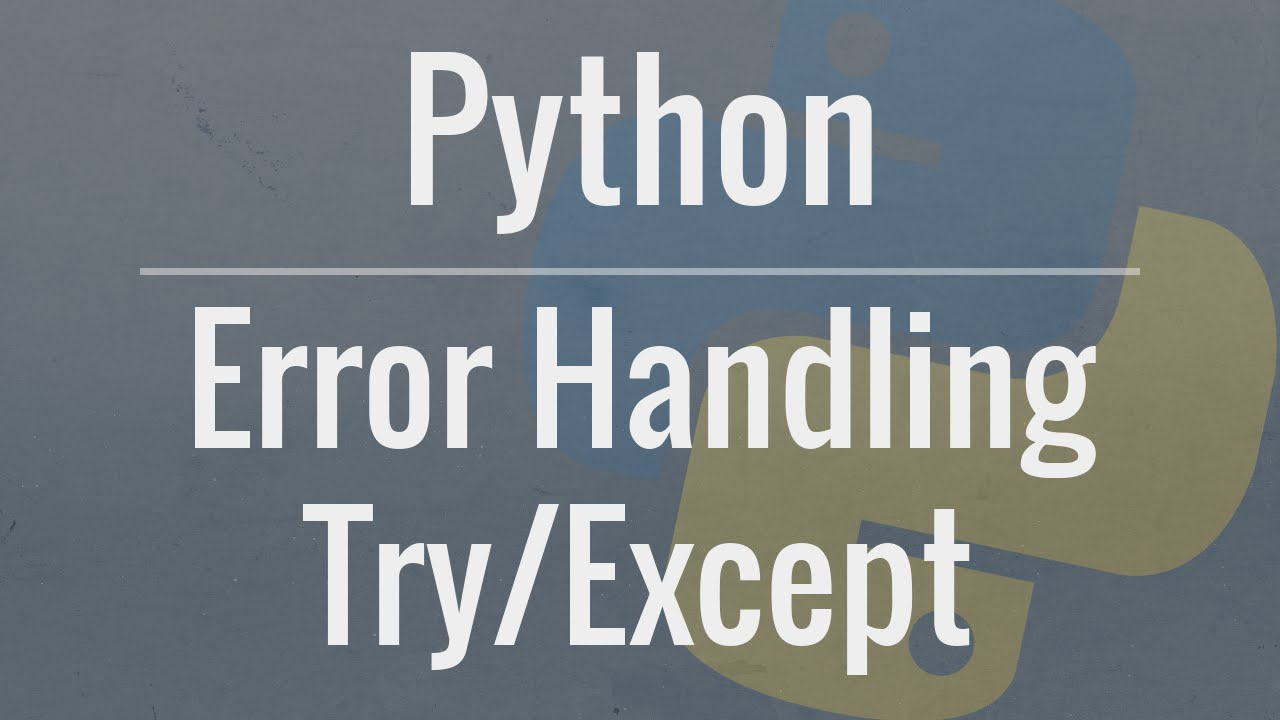
\includegraphics[width=0.60\textwidth]{Gambar/dapi6.jpg}}
 	\caption{Python Exceptions Handling}
 	\label{Python Exceptions Handling}
 \end{figure}
 
 
 
 \section {Pengertian }
 \subsection {Python Exceptions Handling}
 
 
 \hspace*{0.64in} Python menyediakan dua fitur yang sangat penting untuk menangani kesalahan tak terduga dalam program Python Anda dan menambahkan kemampuan debugging di dalamnya Exception Handling: Ini akan dibahas dalam tutorial ini. Berikut adalah daftar standar Pengecualian yang tersedia dengan Python: Pengecualian Standar. Penegasan: Ini akan dibahas dalam Asertions dengan tutorial Python. Daftar Pengecualian Standar – Penegasan dengan Python Penegasan adalah pemeriksaan kewarasan yang dapat Anda aktifkan atau matikan saat Anda selesai dengan pengujian program Anda. Cara termudah untuk memikirkan sebuah pernyataan adalah menyamakannya dengan pernyataan kenaikan gaji-jika (atau lebih akurat, pernyataan kenaikan-jika-tidak). Sebuah ekspresi diuji, dan jika hasilnya muncul salah, pengecualian akan meningkat. Penegasan dilakukan dengan pernyataan tegas, kata kunci terbaru untuk Python, diperkenalkan di versi 1.5. Pemrogram sering menempatkan asersi pada awal fungsi untuk memeriksa masukan yang valid, dan setelah pemanggilan fungsi untuk memeriksa keluaran yang valid. Pernyataan tegas Ketika menemukan pernyataan tegas, Python mengevaluasi ekspresi yang menyertainya, yang semoga benar. Jika ungkapannya salah, Python menimbulkan pengecualian AssertionError. Sintaks untuk menegaskan adalah -menegaskan Ekspresi [, Argumen]. 
 
 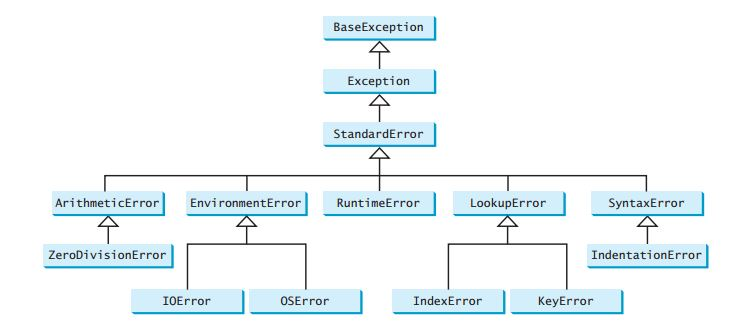
\includegraphics[width=15cm,height=7cm]{Gambar/dapi5.jpg}
 \begin{equation}Python Exceptions Handling\end{equation}
 

\section{Kelas dasar untuk semua pengecualian } 

\subsection{EXCEPTION NAME }

\vspace{12pt}
 \begin{enumerate}
\item StopIteration 

Dibesarkan ketika metode (iterator) berikutnya dari iterator tidak mengarah ke objek apa pun. 
\vspace{12pt}

\item SystemExit 
Dibesarkan oleh fungsi sys.exit () 
\vspace{12pt}

\item StandardError 
 
Kelas dasar untuk semua pengecualian built-in kecuali StopIteration dan SystemExit 
\vspace{12pt}

\item ArithmeticError 
 
Kelas dasar untuk semua kesalahan yang terjadi untuk perhitungan numerik. 
\vspace{12pt}

\item OverflowError 

Dibesarkan saat perhitungan melebihi batas maksimum untuk tipe numerik.
\vspace{12pt}

\item FloatingPointError   

Dibesarkan saat perhitungan floating point gagal. 
\vspace{12pt}

\item ZeroDivisionError  

Dibesarkan saat pembagian atau modulo nol dilakukan untuk semua tipe numerik. 
\vspace{12pt}
\vspace{12pt}

\item AssertionError 

Dibesarkan jika terjadi kegagalan pernyataan Assert. 
\vspace{12pt}

\item AttributeError 
 
Dibesarkan jika terjadi kegagalan referensi atribut atau penugasan.
\vspace{12pt}

\item EOFError 

Dibesarkan bila tidak ada input dari fungsi raw $  \_  $input () atau input () dan akhir file tercapai. 
\vspace{12pt}

\item ImportError 

Dibesarkan saat sebuah pernyataan impor gagal. 
\vspace{12pt}

\item KeyboardInterrupt  

Dibesarkan saat pengguna menyela eksekusi program, biasanya dengan menekan Ctrl + c. 
\vspace{12pt}

\item LookupError  

Kelas dasar untuk semua kesalahan pencarian. 
\vspace{12pt}


\item KeyError 
 
Dibesarkan saat sebuah indeks tidak ditemukan secara berurutan. Dibesarkan saat kunci yang ditentukan tidak ditemukan dalam kamus. 
\vspace{12pt}

\item NameError 

Dibesarkan saat pengenal tidak ditemukan di namespace lokal atau global. 
\vspace{12pt}



\item EnvironmentError  
 
Dibesarkan saat mencoba mengakses variabel lokal dalam suatu fungsi atau metode namun tidak nilai yang ditugaskan padanya. Kelas dasar untuk semua pengecualian yang terjadi di luar lingkungan Python. 
\vspace{12pt}


\item IOError 

IOError Dibesarkan saat operasi input / output gagal, seperti pernyataan cetak atau fungsi open () saat mencoba membuka file yang tidak ada. Dibangkitkan untuk kesalahan terkait sistem operasi. 
\vspace{12pt}

\end {enumerate}
 
\section{SyntaxError} 

\begin{enumerate}


\item IndentationError 

Dibesarkan saat ada kesalahan dengan sintaks Python. Dibesarkan saat indentasi tidak ditentukan dengan benar. 


\item SystemError  

Dibesarkan saat penafsir menemukan masalah internal, namun bila kesalahan ini ditemui juru bahasa Python tidak keluar. 
\vspace{12pt}




\item SystemExit  

Dibesarkan saat juru bahasa Python berhenti dengan menggunakan fungsi sys.exit (). Jika tidak ditangani dalam kode, menyebabkan penafsir untuk keluar. 
\vspace{12pt}


\item TypeError 

Dibesarkan saat operasi atau fungsi dicoba yang tidak valid untuk tipe data yang ditentukan. 
\vspace{12pt}


\item ValueError 

Dibesarkan saat fungsi bawaan untuk tipe data memiliki jenis argumen yang valid, namun argumen tersebut memiliki nilai yang tidak valid yang ditentukan. 
\vspace{12pt}

\item RuntimeError 

Dibesarkan saat kesalahan yang dihasilkan tidak termasuk dalam kategori apa pun. 
\vspace{12pt}

 \end {enumerate}

 \hspace*{0.5in} Jika asersi gagal, Python menggunakan ArgumentExpression sebagai argumen untuk AssertionError. Penegasan Pengecualian pengecualian dapat ditangkap dan ditangani seperti pengecualian lainnya dengan menggunakan perintah try-except, namun jika tidak ditangani, mereka akan menghentikan program dan menghasilkan traceback. 
 
Contoh Berikut adalah fungsi yang mengubah suhu dari derajat Kelvin sampai derajat Fahrenheit. Karena nol derajat Kelvin sedingin yang didapatnya, fungsi itu mundur jika melihat suhu negatif –
\vspace{12pt}
\begin{verbatim}
 $  \#  $!/usr/bin/python 
 
def KelvinToFahrenheit(Temperature): 

~~ assert (Temperature >= 0),"Colder than absolute zero!" 

~~ return ((Temperature-273)*1.8)+32 

print KelvinToFahrenheit(273) 

print int(KelvinToFahrenheit(505.78)) 

print KelvinToFahrenheit(-5) 
\vspace{14pt}

Bila kode diatas dieksekusi, maka menghasilkan hasil sebagai berikut – 
\vspace{12pt}

32.0 

451 

Traceback (most recent call last): 

File "test.py", line 9, in  

print KelvinToFahrenheit(-5) 

File "test.py", line 4, in KelvinToFahrenheit

assert (Temperature >= 0),"Colder than absolute zero!" 

AssertionError: Colder than absolute zero! 
\vspace{12pt}
\end{verbatim}
Apa itu Exception? 

Pengecualian adalah sebuah peristiwa, yang terjadi selama pelaksanaan program yang mengganggu aliran normal instruksi program. Secara umum, ketika skrip Python menemukan situasi yang tidak dapat diatasi, hal itu menimbulkan pengecualian. Pengecualian adalah objek Python yang mewakili kesalahan. 
\vspace{12pt}

Ketika skrip Python menimbulkan pengecualian, ia harus menangani pengecualian begitu saja sehingga berhenti dan berhenti. Menangani pengecualian Jika Anda memiliki beberapa kode yang mencurigakan yang mungkin menimbulkan pengecualian, Anda dapat mempertahankan program Anda dengan menempatkan kode yang mencurigakan di coba: blokir. Setelah dicoba: blokir, sertakan sebuah pernyataan kecuali:, diikuti oleh blok kode yang menangani masalah ini seaman mungkin. Sintaksis Berikut adalah sintaks sederhana coba .... kecuali ... blok lain – 
\vspace{12pt}

\begin{verbatim}
try: 

~~ You do your operations here; 

~~ ...................... 

except \textit{ExceptionI}: 

~~ If there is ExceptionI, then execute this block. 

except \textit{ExceptionII}: 

~~ If there is ExceptionII, then execute this block. 

~~ ...................... 

else: 

~~ If there is no exception then execute this block 
\vspace{12pt}
\vspace{12pt}

\end{verbatim}

Berikut adalah beberapa poin penting tentang sintaks yang disebutkan di atas - 

 \hspace*{0.5in} \vspace{12pt}
\vspace{12pt}

 \hspace*{0.5in} Pernyataan percobaan tunggal dapat memiliki banyak kecuali pernyataan. Ini berguna saat blok coba berisi pernyataan yang mungkin membuang berbagai jenis pengecualian. $  $Anda juga bisa memberikan klausa umum kecuali klausul, yang menangani pengecualian apapun.Setelah klausa kecuali, Anda bisa memasukkan klausul lain. Kode di blok yang lain dijalankan jika kode di coba: blok tidak menimbulkan pengecualian.Blok yang lain adalah tempat yang baik untuk kode yang tidak perlu dicoba: perlindungan blokir. Contoh Contoh ini membuka file, menulis konten di file, dan keluar dengan anggun karena tidak ada masalah sama sekali - 
\vspace{16pt}

\begin{verbatim}

 $  \#  $!/usr/bin/python 
\vspace{12pt}
 
try: 

~~ fh = open("testfile", "w") 

~~ fh.write("This is my test file for exception handling!!") 

except IOError: 

~~ print "Error: can $  \setminus  $'t find file or read data" 

else: 

~~ print "Written content in the file successfully" 

~~ fh.close() 
\vspace{16pt}

Ini menghasilkan hasil sebagai berikut - 
\vspace{12pt}

Written content in the file successfully 
\vspace{12pt}
 
 \end{verbatim}
 
Klausul kecuali tanpa pengecualian anda juga dapat menggunakan pernyataan kecuali tanpa pengecualian yang didefinisikan sebagai berikut - 
\vspace{12pt}

\begin{verbatim}

try: 

~~ You do your operations here; 

~~ ...................... 

except:

~~ If there is any exception, then execute this block. 

~~ ...................... 

else: 

~~ If there is no exception then execute this block.  
\vspace{12pt}
\vspace{16pt}

\end{verbatim}

 \hspace*{0.5in} Pernyataan try-except semacam ini menangkap semua pengecualian yang terjadi. Dengan menggunakan jenis try-except statement ini tidak dianggap sebagai praktik pemrograman yang bagus, karena menangkap semua pengecualian namun tidak membuat programmer mengenali akar permasalahan yang mungkin terjadi. Klausul Kecuali dengan Beberapa Pengecualian Anda juga dapat menggunakan pernyataan kecuali yang sama untuk menangani beberapa pengecualian sebagai berikut - 
\vspace{12pt}
 
try: 

~~ You do your operations here; 

~~ ...................... 

except(Exception1[, Exception2[,...ExceptionN]]]): 

~~ If there is any exception from the given exception list,  

~~ then execute this block. 

~~ ...................... 

else: 

~~ If there is no exception then execute this block.  
\vspace{12pt}
\vspace{12pt}
 
 $  \#  $!/usr/bin/python 
\vspace{12pt}

try: 

~~ fh = open("testfile", "w") 

~~ fh.write("This is my test file for exception handling!!") 
 
finally: 

~~ print "Error: can $  \setminus  $'t find file or read data" 
\vspace{12pt}
\vspace{12pt}
 
 $  \#  $!/usr/bin/python 
\vspace{12pt}
 
try: 

~~ fh = open("testfile", "w") 

~~ try: 
 
~~~~~ fh.write("This is my test file for exception handling!!") 

~~ finally: 

~~~~~ print "Going to close the file" 

~~~~~ fh.close() 

except IOError: 

~~ print "Error: can $  \setminus  $'t find file or read data" 
\vspace{12pt}
\vspace{16pt}

 \hspace*{0.5in} Bila dikecualikan dilempar di blok coba, eksekusi langsung lolos ke blok akhirnya. Setelah semua pernyataan di blok akhirnya dieksekusi, pengecualian dinaikkan lagi dan ditangani dalam pernyataan kecuali jika ada di lapisan yang lebih tinggi dari pernyataan try-except. Argumen Eksepsi Pengecualian dapat memiliki argumen, yang merupakan nilai yang memberi informasi tambahan tentang masalah tersebut. Isi argumen bervariasi menurut pengecualian. Anda menangkap argumen pengecualian dengan menyediakan sebuah variabel dalam klausa kecuali sebagai berikut - 
\vspace{12pt}

try: 

~~ You do your operations here;

~~ ...................... 

except \textit{ExceptionType}\textit{,}\textit{ }\textit{Argument}: 

~~ You can print value of Argument here... 
\vspace{12pt}

 \hspace*{0.5in} Jika Anda menulis kode untuk menangani satu pengecualian, Anda dapat memiliki variabel mengikuti nama pengecualian dalam pernyataan kecuali. Jika Anda menjebak beberapa pengecualian, Anda dapat memiliki variabel mengikuti tuple pengecualian. Variabel ini menerima nilai pengecualian yang sebagian besar mengandung penyebab pengecualian. Variabel tersebut dapat menerima satu nilai atau beberapa nilai dalam bentuk tuple. Tuple ini biasanya berisi error string, error number, dan error location. Pengecualian yang Ditentukan Pengguna Python juga memungkinkan Anda membuat pengecualian sendiri dengan menurunkan kelas dari pengecualian standar built-in. Berikut adalah contoh yang berkaitan dengan RuntimeError. Di sini, sebuah kelas dibuat yang dikelompokkan dari RuntimeError. Ini berguna saat Anda perlu menampilkan informasi yang lebih spesifik saat pengecualian tertangkap. Di blok percobaan, pengecualian yang ditentukan pengguna dinaikkan dan ditangkap di blok kecuali. Variabel e digunakan untuk membuat sebuah instance dari class Networkerror. 
\vspace{12pt}

{\fontsize{10pt}{10pt}\selectfont  (x,y) = (5,0)} 

{\fontsize{10pt}{10pt}\selectfont  try:} 

{\fontsize{10pt}{10pt}\selectfont ~~ z = x/y} 


{\fontsize{10pt}{10pt}\selectfont  except ZeroDivisionError:}


{\fontsize{10pt}{10pt}\selectfont ~~ print "divide by zero"} 

\vspace{10pt}

Jika Anda ingin memeriksa pengecualian dari kode, Anda bisa memiliki: 

\vspace{12pt}
 
\vspace{12pt}

\vspace{12pt}

{\fontsize{10pt}{10pt}\selectfont  (x,y) = (5,0)} 


{\fontsize{10pt}{10pt}\selectfont  try:} 


{\fontsize{10pt}{10pt}\selectfont ~~ z = x/y} 


{\fontsize{10pt}{10pt}\selectfont  except ZeroDivisionError as e:} 

{\fontsize{10pt}{10pt}\selectfont ~~ z = e  $  \#  $ representation: "<exceptions.ZeroDivisionError instance at 0x817426c>"} 


{\fontsize{10pt}{10pt}\selectfont  print z  $  \#  $ output: "integer division or modulo by zero"} 

\vspace{16pt}

General Error Catching 

\vspace{12pt}
 
 \hspace*{0.64in} Terkadang, Anda ingin menangkap semua kesalahan yang mungkin dihasilkan, tapi biasanya Anda tidak melakukannya. Dalam kebanyakan kasus, Anda ingin menjadi sespesifik mungkin (CatchWhatYouCanHandle). Pada contoh pertama di atas, jika Anda menggunakan klausul pengecualian catch-all dan pengguna menekan Ctrl-C, menghasilkan KeyboardInterrupt, Anda tidak ingin program mencetak "bagi dengan nol". Namun, ada beberapa situasi di mana yang terbaik untuk menangkap semua kesalahan. Misalnya, Anda menulis modul ekstensi ke layanan web. Anda ingin informasi kesalahan untuk output output halaman web, dan server untuk terus berjalan, jika mungkin. Tapi Anda tidak tahu kesalahan apa yang mungkin Anda masukkan ke dalam kode Anda. Dalam situasi seperti ini, Anda mungkin ingin mengode sesuatu seperti ini: 
\vspace{12pt}


{\fontsize{10pt}{10pt}\selectfont  import sys}
 

{\fontsize{10pt}{10pt}\selectfont  try:} 


{\fontsize{10pt}{10pt}\selectfont ~~ untrusted.execute()} 


{\fontsize{10pt}{10pt}\selectfont  except:  $  \#  $ catch *all* exceptions} 


{\fontsize{10pt}{10pt}\selectfont ~~ e = sys.exc $  \_  $info()[0]} 


{\fontsize{10pt}{10pt}\selectfont ~~ write $  \_  $to $  \_  $page( "<p>Error:  $  \%  $s</p>"  $  \%  $ e )} 
\vspace{10pt}

 \hspace*{0.64in} Menemukan Nama Pengecualian Spesifik Pengecualian standar yang dapat diajukan dijelaskan secara rinci pada: $  $
 Lihatlah dokumentasi kelas untuk mengetahui pengecualian apa yang bisa diberikan oleh kelas tertentu. Lihat juga: Di wiki ini: WritingExceptionClasses, TracebackModule. Untuk gagasan umum (non-Python specific) tentang pengecualian, berkonsultasilah dengan ExceptionPatterns. Untuk menulis tentang ... 

\vspace{12pt}
 
\begin{itemize}
\item Berikan contoh IOError, dan interpretasikan kode IOError. 

\item Berikan contoh beberapa pengecualian. Penanganan beberapa kecuali dalam satu baris.\end{itemize}
 
 
\vspace{12pt}

Pertanyaan Penanganan Kesalahan Umum, Di bagian "penanganan kesalahan umum" di atas, tertulis untuk menangkap semua pengecualian, Anda menggunakan kode berikut: 
\vspace{14pt}
 
{\fontsize{10pt}{10pt}\selectfont import sys} 


{\fontsize{10pt}{10pt}\selectfont  try:} 

\vspace{10pt}
 

{\fontsize{10pt}{10pt}\selectfont ~~ untrusted.execute()} 

\vspace{10pt}


{\fontsize{10pt}{10pt}\selectfont  except:  $  \#  $ catch *all* exceptions} 

\vspace{10pt}


{\fontsize{10pt}{10pt}\selectfont ~~ e = sys.exc $  \_  $info()[0]} 

\vspace{10pt}


{\fontsize{10pt}{10pt}\selectfont ~~ write $  \_  $to $  \_  $page( "<p>Error:  $  \%  $s</p>"  $  \%  $ e )} 
\vspace{16pt}


{\fontsize{10pt}{10pt}\selectfont  try:}

\vspace{10pt}
 
 
{\fontsize{10pt}{10pt}\selectfont ~~ untrusted.execute()} 

\vspace{10pt}

 
{\fontsize{10pt}{10pt}\selectfont  except Exception as e:} 

\vspace{10pt}

 
{\fontsize{10pt}{10pt}\selectfont ~~ write $  \_  $to $  \_  $page( "<p>Error:  $  \%  $s</p>"  $  \%  $ str(e) )} 
\vspace{16pt}

 \hspace*{0.64in} Seseorang menunjukkan bahwa "kecuali" menangkap lebih dari sekedar "kecuali Pengecualian sebagai e." Mengapa demikian? Apa bedanya? – LionKimbro Untuk saat ini (versi <= 2.4) pengecualian tidak harus diwarisi dari Exception. Jadi polos 'kecuali:'nangkap semua pengecualian, tidak hanya sistem. Pengecualian string adalah salah satu contoh pengecualian yang tidak mewarisi dari Exception. – MikeRovner Saya percaya bahwa pada 2,7, pengecualian masih tidak harus diwariskan dari Exception atau bahkan BaseException. Namun, seperti Python 3, pengecualian harus subclass BaseException. - gajah jim Mendapatkan Informasi Berguna dari Pengecualian Jadi, saya punya sesuatu seperti: 
 
\vspace{12pt}


{\fontsize{10pt}{10pt}\selectfont  (a,b,c) = d} 

\vspace{12pt}
 
dan Python kembali: 
 
\vspace{12pt}
 
 
{\fontsize{10pt}{10pt}\selectfont  ValueError: unpack list of wrong size} 
\vspace{16pt}

... dan begitulah, Anda tentu bertanya-tanya, "Nah, apa yang ada di d?" 

\vspace{12pt}

Anda tahu - Anda bisa mencetak di sana, dan itu berhasil. Tapi adakah cara yang lebih baik dan lebih menarik untuk mendapatkan informasi yang diketahui orang? Anda bisa melakukan sesuatu seperti: 
\vspace{20pt}

 
 try: 
 
 
~~ a, b, c = d 
 
 
 except Exception as e: 
 
 
~~ e.args += (d,) 
 
 
~~ raise 
\vspace{20pt}
 
 \hspace*{0.64in} Atribut .args pengecualian adalah tuple dari semua argumen yang dilewatkan (biasanya argumen satu dan satu-satunya adalah pesan kesalahannya). Dengan cara ini Anda dapat mengubah argumen dan menaikkan kembali, dan informasi tambahan akan ditampilkan. Anda juga bisa membuat pernyataan cetak atau login di blok kecuali. Perhatikan bahwa tidak semua pengecualian subclass Exception (meski hampir semua dilakukan), jadi ini mungkin tidak menangkap beberapa pengecualian; Selain itu, pengecualian tidak diperlukan untuk memiliki atribut .args (meskipun jika pengecualian subclass Exception dan tidak mengesampingkan  $  \_  $ $  \_  $init $  \_  $ $  \_  $ tanpa memanggil superclass-nya), maka kode yang ditulis mungkin gagal Namun dalam prakteknya hampir tidak pernah (dan Jika ya, Anda harus memperbaiki pengecualian yang tidak sesuai!) Bukankah lebih baik mencegahnya untuk melakukan remediasi? >  
 Joel Spolsky mungkin programmer hebat C ++, dan sarannya untuk desain antarmuka pengguna sangat berharga, tapi Python bukan C ++ atau Java, dan argumennya tentang pengecualian tidak berlaku dengan Python. Joel berpendapat: "Mereka tidak terlihat dalam kode sumber Melihat kumpulan kode, termasuk fungsi yang mungkin atau mungkin tidak membuang pengecualian, tidak ada cara untuk melihat pengecualian mana yang mungkin dilempar dan dari mana.Ini berarti bahwa pemeriksaan kode yang hati-hati pun tidak. Saya bisa mengungkapkan potensi bug. " 

 \hspace*{0.64in} (Perhatikan bahwa ini juga merupakan argumen di balik pengecualian yang diperiksa oleh Java - sekarang eksplisit bahwa pengecualian dapat dilemparkan - kecuali bahwa RuntimeException masih dapat dibuang ke mana saja. -jJ) Saya tidak mengerti argumen ini. Dalam kode sumber acak, tidak ada cara untuk mengetahui apakah akan gagal hanya dengan inspeksi. Jika Anda melihat: 

\vspace{12pt}

\vspace{12pt}

x = 1 

result = myfunction (x) 
\vspace{20pt}

 \hspace*{0.64in} Anda tidak dapat mengetahui apakah fungsi saya gagal pada saat runtime hanya dengan inspeksi, jadi mengapa harus itu penting apakah gagal menabrak pada saat runtime atau gagal dengan meningkatkan pengecualian? 
 
\vspace{12pt}
 
(Crashing itu buruk Dengan secara eksplisit menyatakan pengecualian, Anda memperingatkan orang-orang bahwa mereka mungkin ingin mengatasinya Jawa melakukannya dengan canggung C tidak memiliki cara yang baik untuk melakukannya sama sekali, karena kesalahan kembali masih di band Untuk pengembalian reguler Di python, pengecualian passthrough tidak ditandai, namun kondisi kesalahan menonjol di tempat mereka diciptakan, dan biasanya tidak meniru hasil yang benar. -jJ)

 \hspace*{0.64in} Argumen Joel yang mengemukakan pengecualian hanyalah sebuah goto yang menyamar sebagian benar. Tapi begitu juga untuk loop, sementara loop, fungsi dan metode! Seperti konstruksi lainnya, pengecualian adalah gotos yang dijinakkan dan dipekerjakan untuk Anda, bukan yang liar dan berbahaya. Anda tidak bisa melompat * di mana saja *, hanya tempat yang sangat terbatas. 
 
\vspace{12pt}

Joel juga menulis: 

\vspace{12pt}
 
 \hspace*{0.64in} "Mereka membuat terlalu banyak titik keluar yang mungkin untuk sebuah fungsi.Untuk menulis kode yang benar, Anda benar-benar harus memikirkan setiap jalur kode yang mungkin melalui fungsi Anda. Setiap kali Anda memanggil fungsi yang dapat meningkatkan pengecualian dan tidak menangkapnya di Spot, Anda menciptakan peluang untuk kejutan bug yang disebabkan oleh fungsi yang dihentikan tiba-tiba, meninggalkan data dalam keadaan tidak konsisten, atau jalur kode lainnya yang tidak Anda pikirkan. " 
 
\vspace{12pt}
 
\vspace{10pt}
\vspace{12pt}

try: 
 
~~ You do your operations here; 

~~ ...................... 
 
except(Exception1[, Exception2[,...ExceptionN]]]): 
 
~~ If there is any exception from the given exception list,  

~~ then execute this block. 

~~ ...................... 

else: 
 
~~ If there is no exception then execute this block.  
\vspace{12pt}
\vspace{12pt}
 
 $  \#  $!/usr/bin/python 
\vspace{12pt}

try: 
 
~~ fh = open("testfile", "w") 

~~ fh.write("This is my test file for exception handling!!") 

finally: 

~~ print "Error: can $  \setminus  $'t find file or read data" 
\vspace{12pt}
\vspace{12pt}
 
 $  \#  $!/usr/bin/python 
\vspace{12pt}
 
try: 
 
~~ fh = open("testfile", "w") 

~~ try: 
 
~~~~~ fh.write("This is my test file for exception handling!!") 

~~ finally: 
 
~~~~~ print "Going to close the file" 

~~~~~ fh.close() 

except IOError: 
 
~~ print "Error: can $  \setminus  $'t find file or read data" 
\vspace{12pt}
\vspace{12pt}
\vspace{12pt}
\vspace{12pt}
Bila dikecualikan dilempar di blok coba, eksekusi langsung lolos ke blok akhirnya. Setelah semua pernyataan di blok akhirnya dieksekusi, pengecualian dinaikkan lagi dan ditangani dalam pernyataan kecuali jika ada di lapisan yang lebih tinggi dari pernyataan try-except. Argumen Eksepsi. Python juga memungkinkan Anda membuat pengecualian sendiri dengan menurunkan kelas dari pengecualian standar built-in. Berikut adalah contoh yang berkaitan dengan RuntimeError. Di sini, sebuah kelas dibuat yang dikelompokkan dari RuntimeError. Ini berguna saat Anda perlu menampilkan informasi yang lebih spesifik saat pengecualian tertangkap. Di blok percobaan, pengecualian yang ditentukan pengguna dinaikkan dan ditangkap di blok kecuali. Variabel e digunakan untuk membuat sebuah instance dari class Networkerror. 
\vspace{18pt}



\chapter{Clasess/Object}
\section{center}{\fontsize{16pt}{16pt}\selectfont \textbf{Python Object Oriented} \\}\end{center} 
Python telah menjadi bahasa berorientasi objek sejak itu ada. Karena itu, menciptakan dan menggunakan kelas dan objek sangat mudah. Bab ini membantu Anda menjadi ahli dalam menggunakan dukungan pemrograman berorientasi objek Python. Jika Anda tidak memiliki pengalaman sebelumnya dengan pemrograman berorientasi objek (OO), Anda mungkin ingin berkonsultasi dengan kursus perkenalan atau setidaknya tutorial semacam itu sehingga Anda dapat memahami konsep dasarnya. Namun, di sini adalah pengenalan kecil Object-Oriented Programming (OOP) untuk membawa Anda pada kecepatan - Ikhtisar Terminologi OOP. Kelas: Prototipe yang ditentukan pengguna untuk objek yang mendefinisikan seperangkat atribut yang menjadi ciri objek kelas apa pun. Atribut adalah data anggota (variabel kelas dan variabel contoh) dan metode, diakses melalui notasi titik. Variabel kelas: Variabel yang dimiliki oleh semua instance kelas. Variabel kelas didefinisikan dalam kelas tapi di luar metode kelas manapun. Variabel kelas tidak digunakan sesering variabel contoh. Anggota data: Variabel kelas atau variabel contoh yang menyimpan data yang terkait dengan kelas dan objeknya. Fungsi overloading: Penugasan lebih dari satu perilaku ke fungsi tertentu. Operasi yang dilakukan bervariasi menurut jenis objek atau argumen yang terlibat.Contoh variabel: Variabel yang didefinisikan di dalam metode dan hanya dimiliki oleh instance kelas saat ini. 
Warisan: Pengalihan karakteristik kelas ke kelas lain yang berasal darinya. Contoh: Objek individual dari kelas tertentu. Obyek obj yang termasuk dalam Lingkaran kelas, misalnya, adalah turunan dari Lingkaran kelas. Instansiasi: Pembuatan sebuah instance dari sebuah kelas. Metode: Jenis fungsi khusus yang didefinisikan dalam definisi kelas.  Objek: Contoh unik dari struktur data yang didefinisikan oleh kelasnya. Objek terdiri dari kedua anggota data (variabel kelas dan variabel contoh) dan metode. Operator overloading: Penugasan lebih dari satu fungsi ke operator tertentu. 

\subsection{Pernyataan kelas membuat definisi kelas baru}
Pernyataan kelas membuat definisi kelas baru , Nama kelas segera mengikuti kelas kata kunci diikuti oleh titik dua sebagai berikut 
class ClassName: 
~~ 'Optional class documentation string' 
~~ class \$  \_  \$suite 
\subsubsection {Kelas~memiliki kumpulan dokumentasi}
Kelas~memiliki kumpulan dokumentasi, yang bisa diakses melalui ClassName . \$  \_  \$ \$  \_  \$ doc \$  \_  \$ \$  \_  \$.  Class \$  \_  \$ suite terdiri dari semua pernyataan komponen yang mendefinisikan anggota kelas, atribut dan fungsi data. 
Berikut adalah contoh kelas Python sederhana 
class Employee:
~~ 'Common base class for all employees' 
~~ empCount = 0 
~~ def  \$  \_  \$ \  \_  \$init \$  \_  \$ \$  \_  \$(self, name, salary):  
~~~~~ self.name = name  
~~~~~ self.salary = salary 
~~~~~ Employee.empCount += 1 
~~  
~~ def displayCount(self): \
~~~~ print "Total Employee  \$  \%  \$d"  \$  \%  \$ Employee.empCount 
~~ def displayEmployee(self):
~~~~~~print "Name : ", self.name,  ", Salary: ", self.salary 
Variabel empCount adalah variabel kelas yang nilainya dibagi di antara semua contoh kelas ini. Ini bisa diakses sebagai Employee.empCount dari dalam kelas atau di luar kelas. Metode pertama  \$  \_  \$ \$  \_  \$init  \$  \_  \$ \$  \_  \$ () adalah metode khusus, yang disebut metode konstruktor kelas atau inisialisasi yang Python panggil saat Anda membuat instance baru dari kelas ini. Anda menyatakan metode kelas lain seperti fungsi normal dengan pengecualian bahwa argumen pertama untuk setiap metode adalah self. Python menambahkan argumen diri ke daftar untuk Anda; Anda tidak perlu memasukkannya saat Anda memanggil metode. 
{\fontsize{14pt}{14pt}\selectfont \textbf{Membuat Instance Objects} \\} 
Untuk membuat contoh kelas, Anda memanggil kelas menggunakan nama kelas dan meneruskan argumen apa pun yang diterima metode  \$  \_  \$ \$  \_  \$init \$  \_  \$ \$  \_  \$-nya. 
"Ini akan menciptakan objek pertama kelas Karyawan" 
Emp1 = Karyawan ("Zara", 2000) 
"Ini akan menciptakan objek kedua dari kelas Karyawan" 
Emp2 = Karyawan ("Manni", 5000) 
{\fontsize{14pt}{14pt}\selectfont \textbf{Mengakses Atribut} \\}
Anda mengakses atribut objek menggunakan dot operator dengan objek. Variabel kelas akan diakses dengan menggunakan nama kelas sebagai berikut 
Emp1.displayEmployee () 
Emp2.displayEmployee ()  
Cetak "Jumlah Karyawan \$  \%  \$ d" \$  \%  \$ Employee.empCount 
Sekarang, meletakkan semua konsep bersama 
 \$  \#  \$!/usr/bin/python 
class Employee: 
~~ 'Common base class for all employees' 
~~ empCount = 0 
~~ def  \$  \_  \$ \$  \_  \$init \$  \_  \$ \$  \_  \$(self, name, salary): 
~~~~~ self.name = name \par
~~~~~ self.salary = salary \par
~~~~~ Employee.empCount += 1 \par
~~  \par
\noindent 
~~ def displayCount(self): \par
\noindent 
~~~~ print "Total Employee  \$  \%  \$d"  \$  \%  \$ Employee.empCount \par
\vspace{12pt}
\noindent 
~~ def displayEmployee(self): \par
\noindent 
~~~~~~print "Name : ", self.name,  ", Salary: ", self.salary \par
\vspace{12pt}
\noindent 
"This would create first object of Employee class" \par
\noindent 
emp1 = Employee("Zara", 2000) \par
\noindent 
"This would create second object of Employee class" \par
\noindent 
emp2 = Employee("Manni", 5000) \par
\noindent 
emp1.displayEmployee() \par
\noindent 
emp2.displayEmployee() \par
\noindent 
print "Total Employee  \$  \%  \$d"  \$  \%  \$ Employee.empCount \par
\noindent 
When the above code is executed, it produces the following result  \$ - \$ \par
\noindent 
Name~:~ Zara ,Salary:  2000 \par
\noindent 
Name~:~ Manni ,Salary:  5000 \par
\noindent 
Total Employee 2 \par
\noindent 
You can add, remove, or modify attributes of classes and objects at any time  $ - $ \par
\noindent 
emp1.age~= 7   \$  \#  \$ Add an 'age' attribute. \par
\noindent 
emp1.age~= 8   \$  \#  \$ Modify 'age' attribute. \par
\noindent 
del~emp1.age   \$  \#  \$ Delete 'age' attribute. \par
\vspace{12pt}
Alih-alih menggunakan pernyataan normal untuk mengakses atribut, Anda dapat menggunakan fungsi berikut - \par
\vspace{12pt}
\noindent 
~~~ Getattr (obj, name [, default]): untuk mengakses atribut objek. \par
\vspace{12pt}
\noindent 
~~~ Hasattr (obj, name): untuk memeriksa apakah ada atribut atau tidak. \par
\vspace{12pt}
\noindent 
~~~ Setattr (obj, name, value): untuk mengatur atribut. Jika atribut tidak ada, maka akan dibuat. \par
\vspace{12pt}
\noindent 
~~~ The delattr (obj, name): untuk menghapus sebuah atribut. \par
\vspace{12pt}
\noindent 
Hasattr (emp1, 'age')  \$  \#  \$ Mengembalikan true jika atribut 'age' ada \par
\noindent 
Getattr (emp1, 'age')  \$  \#  \$ Mengembalikan nilai atribut 'age' \par
\noindent 
Setattr (emp1, 'age', 8)  \$  \#  \$ Set attribute 'age' di 8 \par
\noindent 
Delattr (empl, 'age')  \$  \#  \$ Hapus atribut 'umur' \par
\vspace{12pt}
\noindent 
Atribut Atribut Built-In \par
\vspace{12pt}
\noindent 
Setiap kelas Python terus mengikuti atribut bawaan dan mereka dapat diakses menggunakan operator dot seperti atribut lainnya - \par
\vspace{12pt}
\noindent 
~~~  \$  \_  \$ \$  \_  \$dict \$  \_  \$ \$  \_  \$: Kamus yang berisi namespace kelas. \par
\vspace{12pt}
\noindent 
~~~  \$  \_  \$ \$  \_  \$doc \$  \_  \$ \$  \_  \$: String dokumentasi kelas atau tidak, jika tidak terdefinisi. \par
\vspace{12pt}
\noindent 
~~~  \$  \_  \$ \$  \_  \$name \$  \_  \$ \$  \_  \$: nama kelas \par
\vspace{12pt}
\noindent 
~~~  \$  \_  \$ \$  \_  \$module \$  \_  \$ \$  \_  \$: Nama modul dimana kelas didefinisikan. Atribut ini " \$  \_  \$ \$  \_  \$main \$  \_  \$ \$  \_  \$" dalam mode interaktif. \par
\vspace{12pt}
\noindent 
~~~  \$  \_  \$ \$  \_  \$bases\$  \_  \$ \$  \_  \$: Tupel yang mungkin kosong yang berisi kelas dasar, sesuai urutan kejadiannya dalam daftar kelas dasar. \par
\vspace{12pt}
\noindent 
Untuk kelas di atas mari kita coba untuk mengakses semua atribut ini – \par
\vspace{12pt}
\noindent 
 \$  \#  \$!/usr/bin/python \par
\vspace{12pt}
\noindent 
class Employee: \par
\noindent 
~~ 'Common base class for all employees' \par
\noindent 
~~ empCount = 0 \par
\vspace{12pt}
\noindent 
~~ def  $  \_  $ $  \_  $init $  \_  $ $  \_  $(self, name, salary): \par
\noindent 
~~~~~ self.name = name \par
\noindent 
~~~~~ self.salary = salary \par
\noindent 
~~~~~ Employee.empCount += 1 \par
\noindent 
~~  \par
\noindent 
~~ def displayCount(self): \par
\noindent 
~~~~ print "Total Employee  $  \%  $d"  $  \%  $ Employee.empCount \par
\vspace{12pt}
\noindent 
~~ def displayEmployee(self): \par
\noindent 
~~~~~~print "Name : ", self.name,  ", Salary: ", self.salary \par
\vspace{12pt}
\noindent 
print "Employee. $  \_  $ $  \_  $doc $  \_  $ $  \_  $:", Employee. $  \_  $ $  \_  $doc $  \_  $ $  \_  $ \par
\noindent 
print "Employee. $  \_  $ $  \_  $name $  \_  $ $  \_  $:", Employee. $  \_  $ $  \_  $name $  \_  $ $  \_  $ \par
\noindent 
print "Employee. $  \_  $ $  \_  $module $  \_  $ $  \_  $:", Employee. $  \_  $ $  \_  $module $  \_  $ $  \_  $ \par
\noindent 
print "Employee. $  \_  $ $  \_  $bases $  \_  $ $  \_  $:", Employee. $  \_  $ $  \_  $bases $  \_  $ $  \_  $ \par
\noindent 
print "Employee. $  \_  $ $  \_  $dict $  \_  $ $  \_  $:", Employee. $  \_  $ $  \_  $dict $  \_  $ $  \_  $ \par
\vspace{12pt}
\vspace{12pt}
\noindent 
Bila kode diatas dieksekusi, maka menghasilkan hasil sebagai berikut - \par
\vspace{12pt}
\noindent 
Karyawan . $  \_  $ $  \_  $ doc $  \_  $ $  \_  $: kelas dasar umum untuk semua karyawan \par
\noindent 
Karyawan . $  \_  $ $  \_  $ name $  \_  $ $  \_  $: Karyawan \par
\noindent 
Karyawan . $  \_  $ $  \_  $ modul $  \_  $ $  \_  $:  $  \_  $ $  \_  $main $  \_  $ $  \_  $ \par
\noindent 
Karyawan . $  \_  $ $  \_  $ bases $  \_  $ $  \_  $: () \par
\noindent 
Karyawan . $  \_  $ $  \_  $ dict $  \_  $ $  \_  $:  $  \{  $' $  \_  $ $  \_  $module $  \_  $ $  \_  $': ' $  \_  $ $  \_  $main $  \_  $ $  \_  $', 'displayCount': \par
\noindent 
<function displayCount at 0xb7c84994>, 'empCount': 2, \par
\noindent 
'DisplayEmployee': <function displayEmployee at 0xb7c8441c>, \par
\noindent 
' $  \_  $ $  \_  $doc $  \_  $ $  \_  $': 'Kelas dasar umum untuk semua karyawan', \par
\noindent 
' $  \_  $ $  \_  $init $  \_  $ $  \_  $': <function  $  \_  $ $  \_  $init $  \_  $ $  \_  $ di 0xb7c846bc> $  \}  $ \par
\vspace{12pt}
\noindent 
{\fontsize{14pt}{14pt}\selectfont \textbf{Menghancurkan Objek (Pengumpulan Sampah)} \\} \par
\vspace{12pt}
Python menghapus objek yang tidak dibutuhkan (tipe built-in atau instance kelas) secara otomatis untuk membebaskan ruang memori. Proses dimana Python secara berkala mengumpulkan kembali blok memori yang tidak lagi digunakan disebut Koleksi Sampah. Pengumpul sampah Python berjalan selama eksekusi program dan dipicu saat penghitungan referensi objek mencapai nol. Jumlah referensi referensi berubah karena jumlah alias yang menunjukkannya berubah. Jumlah referensi objek meningkat saat diberi nama baru atau ditempatkan dalam wadah (daftar, tupel, atau kamus). Jumlah referensi objek berkurang saat dihapus dengan del, rujukannya ditugaskan kembali, atau rujukannya tidak sesuai. Ketika penghitungan referensi objek mencapai nol, Python mengumpulkannya secara otomatis. \par
\vspace{12pt}
\noindent 
a = 40  $  \#  $ Buat objek <40> \par
\noindent 
B = a  $  \#  $ Tingkatkan ref. Hitung <40> \par
\noindent 
c = [b]  $  \#  $ Tingkatkan ref. Hitung <40> \par
\vspace{12pt}
\noindent 
Del  $  \#  $ Penurunan ref. Hitung <40> \par
\noindent 
b = 100  $  \#  $ Kurangi ref. Hitung <40> \par
\noindent 
C [0] = -1  $  \#  $ Kurangi ref. Hitung <40> \par
\vspace{12pt}
Anda biasanya tidak akan memperhatikan kapan pengumpul sampah menghancurkan contoh yatim piatu dan mengembalikan ruangnya. Tapi kelas bisa menerapkan metode khusus  $  \_  $ $  \_  $del  $  \_  $ $  \_  $ (), yang disebut destructor, yang dipanggil saat instance tersebut hendak dimusnahkan. Metode ini bisa digunakan untuk membersihkan sumber daya non memori yang digunakan oleh sebuah instance. \par
\noindent 
Contoh \par
\vspace{12pt}
\noindent 
Penghancur  $  \_  $ $  \_  $del  $  \_  $ $  \_  $ () ini mencetak nama kelas sebuah instance yang akan dihancurkan - \par
\noindent 
 $  \#  $!/usr/bin/python \par
\vspace{12pt}
\noindent 
class Point: \par
\noindent 
~~ def  $  \_  $ $  \_  $init $  \_  $ $  \_  $( self, x=0, y=0): \par
\noindent 
~~~~~ self.x = x \par
\noindent 
~~~~~ self.y = y \par
\noindent 
~~ def  $  \_  $ $  \_  $del $  \_  $ $  \_  $(self): \par
\noindent 
~~~~~ class $  \_  $name = self. $  \_  $ $  \_  $class $  \_  $ $  \_  $. $  \_  $ $  \_  $name $  \_  $ $  \_  $ \par
\noindent 
~~~~~ print class $  \_  $name, "destroyed" \par
\vspace{12pt}
\noindent 
pt1 = Point() \par
\noindent 
pt2 = pt1 \par
\noindent 
pt3 = pt1 \par
\noindent 
print id(pt1), id(pt2), id(pt3)  $  \#  $ prints the ids of the obejcts \par
\noindent 
del pt1 \par
\noindent 
del pt2 \par
\noindent 
del pt3 \par
\vspace{12pt}
\vspace{12pt}
\noindent 
{\fontsize{14pt}{14pt}\selectfont \textbf{Kelas Warisan} \\} \par
\vspace{12pt}
Alih-alih mulai dari nol, Anda dapat membuat kelas dengan menurunkannya dari kelas yang sudah ada sebelumnya dengan mencantumkan kelas induk dalam tanda kurung setelah nama kelas yang baru. Kelas anak mewarisi atribut kelas induknya, dan Anda dapat menggunakan atribut tersebut seolah-olah mereka didefinisikan di kelas anak. Kelas anak juga dapat mengesampingkan data anggota dan metode dari orang tua. Sintaksis Kelas turunan dinyatakan seperti kelas orang tua mereka; Namun, daftar kelas dasar yang diwarisi dari diberikan setelah nama kelas - \par
\vspace{12pt}
\noindent 
Kelas SubClassName (ParentClass1 [, ParentClass2, ...]): \par
\noindent 
~~ 'String dokumentasi kelas opsional' \par
\noindent 
~~ Class $  \_  $suite \par
\noindent 
 $  \#  $!/usr/bin/python \par
\vspace{12pt}
\noindent 
class~Parent:~~~~~~   $  \#  $ define parent class \par
\noindent 
~~ parentAttr = 100 \par
\noindent 
~~ def  $  \_  $ $  \_  $init $  \_  $ $  \_  $(self): \par
\noindent 
~~~~~ print "Calling parent constructor" \par
\vspace{12pt}
\noindent 
~~ def parentMethod(self): \par
\noindent 
~~~~~ print 'Calling parent method' \par
\vspace{12pt}
\noindent 
~~ def setAttr(self, attr): \par
\noindent 
~~~~~ Parent.parentAttr = attr \par
\vspace{12pt}
\noindent 
~~ def getAttr(self): \par
\noindent 
~~~~~ print "Parent attribute :", Parent.parentAttr \par
\vspace{12pt}
\noindent 
class Child(Parent):  $  \#  $ define child class \par
\noindent 
~~ def  $  \_  $ $  \_  $init $  \_  $ $  \_  $(self): \par
\noindent 
~~~~~ print "Calling child constructor" \par
\vspace{12pt}
\noindent 
~~ def childMethod(self): \par
\noindent 
~~~~~ print 'Calling child method' \par
\vspace{12pt}
\noindent 
c~=~Child()~~~~~~~    $  \#  $ instance of child \par
\noindent 
c.childMethod()~~~~~  $  \#  $ child calls its method \par
\noindent 
c.parentMethod()~~~~  $  \#  $ calls parent's method \par
\noindent 
c.setAttr(200)~~~~~~  $  \#  $ again call parent's method \par
\noindent 
c.getAttr()~~~~~~~~~  $  \#  $ again call parent's method \par
\vspace{12pt}
\noindent 
Calling child constructor \par
\noindent 
Calling child method \par
\noindent 
Calling parent method \par
\noindent 
Parent attribute : 200 \par
\vspace{12pt}
\noindent 
class~A:~~~~~~   $  \#  $ define your class A \par
\noindent 
..... \par
\vspace{12pt}
\noindent 
class~B:~~~~~~~   $  \#  $ define your class B \par
\noindent 
..... \par
\vspace{12pt}
\noindent 
class~C(A,~B):    $  \#  $ subclass of A and B \par
\vspace{12pt}
Anda dapat menggunakan fungsi issubclass () atau isinstance () untuk memeriksa hubungan dua kelas dan contoh. Fungsi boolean issubclass (sub, sup) mengembalikan true jika sub subclass yang diberikan memang merupakan subclass dari superclass sup. The isinstance (obj, Class) fungsi boolean mengembalikan true jika obj adalah turunan dari Class Class atau merupakan instance dari subclass of Class. \par
\vspace{12pt}
\noindent 
{\fontsize{14pt}{14pt}\selectfont \textbf{Metode utama} \\} \par
\vspace{12pt}
Anda selalu dapat mengganti metode kelas induk Anda. Salah satu alasan untuk mengesampingkan metode orang tua adalah karena Anda mungkin menginginkan fungsi khusus atau berbeda di subkelas Anda. \par
Contoh \par
\vspace{12pt}
\noindent 
 $  \#  $! / Usr / bin / python \par
\vspace{12pt}
\noindent 
class parent:  $  \#  $ define parent class \par
\noindent 
~~ Def myMethod (diri): \par
\noindent 
~~~~~ Cetak 'metode induk panggilan' \par
\vspace{12pt}
\noindent 
Kelas anak (orang tua):  $  \#  $ define child class \par
\noindent 
~~ Def myMethod (diri): \par
\noindent 
~~~~~ Cetak 'metode memanggil anak' \par
\vspace{12pt}
\noindent 
C = Anak ()  $  \#  $ contoh anak \par
\noindent 
C.myMethod ()  $  \#  $ metode panggilan balik anak \par
\vspace{12pt}
\noindent 
Bila kode diatas dieksekusi, maka menghasilkan hasil sebagai berikut - \par
\vspace{12pt}
\noindent 
Memanggil metode anak \par
\vspace{12pt}
\noindent 
Metode Base Overloading \par
\vspace{12pt}
\noindent 
Berikut daftar tabel beberapa fungsionalitas generik yang dapat Anda timpa di kelas Anda sendiri - \par
\vspace{14pt}
\noindent 
{\fontsize{14pt}{14pt}\selectfont \textbf{Operator overloading} \\} \par
\vspace{12pt}
Misalkan Anda telah membuat kelas Vektor untuk mewakili vektor dua dimensi, apa yang terjadi bila Anda menggunakan operator plus untuk menambahkannya? Kemungkinan besar Python akan berteriak pada Anda. Anda bisa, bagaimanapun, menentukan metode  $  \_  $ $  \_  $add $  \_  $ $  \_  $ di kelas Anda untuk melakukan penambahan vektor dan operator plus akan berperilaku sesuai harapan - \par
Contoh \par
\vspace{12pt}
\noindent 
 $  \#  $! / Usr / bin / python \par
\vspace{12pt}
\noindent 
Kelas vektor: \par
\noindent 
~~ def  $  \_  $ $  \_  $init  $  \_  $ $  \_  $ (diri, a, b): \par
\noindent 
~~~~~ Self.a = a \par
\noindent 
~~~~~ Self.b = b \par
\vspace{12pt}
\noindent 
~~ def  $  \_  $ $  \_  $str  $  \_  $ $  \_  $ (diri): \par
\noindent 
~~~~~ Return 'Vector ( $  \%  $ d, $  \%  $ d)' $  \%  $ (self.a, self.b) \par
\noindent 
~~  \par
\noindent 
~~ Def  $  \_  $ $  \_  $add  $  \_  $ $  \_  $ (diri sendiri, lainnya): \par
\noindent 
~~~~~ return Vector (self.a + other.a, self.b + other.b) \par
\vspace{12pt}
\noindent 
v1 = vektor (2,10) \par
\noindent 
v2 = vektor (5, -2) \par
\noindent 
cetak v1 + v2 \par
\vspace{12pt}
\noindent 
Bila kode diatas dieksekusi, maka menghasilkan hasil sebagai berikut - \par
\vspace{12pt}
\noindent 
Vektor (7,8) \par
\vspace{12pt}
\noindent 
{\fontsize{14pt}{14pt}\selectfont \textbf{Persembunyian data} \\} \par
\vspace{12pt}
Atribut objek mungkin atau mungkin tidak terlihat di luar definisi kelas. Anda perlu memberi nama atribut dengan awalan ganda ganda, dan atribut tersebut kemudian tidak langsung terlihat oleh orang luar. \par
Contoh \par
\vspace{12pt}
\noindent 
 $  \#  $! / Usr / bin / python \par
\vspace{12pt}
\noindent 
Kelas JustCounter: \par
\noindent 
~~  $  \_  $ $  \_  $secretCount = 0 \par
\noindent 
~  \par
\noindent 
~~ def menghitung (diri): \par
\noindent 
~~~~~ self . $  \_  $ $  \_  $ secretCount + = 1 \par
\noindent 
~~~~~ cetak diri . $  \_  $ $  \_  $ secretCount \par
\vspace{12pt}
\noindent 
counter = JustCounter () \par
\noindent 
Counter.count () \par
\noindent 
Counter.count () \par
\noindent 
print counter . $  \_  $ $  \_  $ secretCount \par
\vspace{12pt}
\noindent 
Bila kode diatas dieksekusi, maka menghasilkan hasil sebagai berikut - \par
\vspace{12pt}
\noindent 
1 \par
\noindent 
2 \par
\noindent 
Traceback (panggilan terakhir): \par
\noindent 
~ File "test.py", baris 12, di <module> \par
\noindent 
~~~ print counter . $  \_  $ $  \_  $ secretCount \par
\noindent 
AttributeError: instance JustCounter tidak memiliki atribut ' $  \_  $ $  \_  $secretCount' \par
\vspace{12pt}
Python melindungi anggota tersebut dengan mengganti namanya secara internal untuk memasukkan nama kelas. Anda dapat mengakses atribut seperti object. $  \_  $className $  \_  $ $  \_  $attrName. Jika Anda akan mengganti baris terakhir Anda sebagai berikut, maka akan berhasil untuk Anda - \par
\vspace{12pt}
\noindent 
print counter. $  \_  $JustCounter $  \_  $ $  \_  $secretCount \par
\vspace{12pt}
\noindent 
Bila kode diatas dieksekusi, maka menghasilkan hasil sebagai berikut - \par
\vspace{12pt}
\noindent 
1 \par
\noindent 
2 \par
\noindent 
2 \par
\vspace{12pt}
Contoh \par
\vspace{12pt}
Kelas bisa mewarisi kelas lainnya. Kelas dapat mewarisi atribut dan perilaku (metode) dari kelas lain, yang disebut kelas super. Sebuah kelas yang mewarisi dari kelas super disebut Sub-kelas. Kelas super kadang disebut nenek moyang juga. Ada hubungan hierarki antar kelas. Jika kita melihat lebih dekat contoh sebelumnya tentang akun kelas, kita dapat melihat bahwa model ini dapat memenuhi kebutuhan bank sebenarnya. Bank biasanya memiliki jenis akun yang berbeda, mis. Rekening Tabungan, Rekening Giro dan lain-lain. Meskipun jenis akun yang berbeda ini sangat berbeda, namun tetap memiliki banyak sifat dan metode yang sama. Misalnya. Setiap akun memiliki dan membutuhkan nomor rekening, pemegang dan saldo. Selanjutnya mungkin bagi masing-masing untuk menyetor atau menarik uang. \par
Jadi, ada sesuatu seperti akun "mendasar" darimana mereka mewarisi. Warisan digunakan untuk membuat kelas baru dengan menggunakan kelas yang ada. Yang baru dapat diciptakan dengan memperluas dan dengan membatasi kelas yang ada. \par
Sekarang saatnya untuk kembali ke Python dan melihat bagaimana kelas diimplementasikan dengan Python. Kita mulai dengan kelas yang paling sederhana, yang bisa didefinisikan. Kami hanya memberikan nama tapi menghilangkan semua spesifikasi lebih lanjut dengan menggunakan kata kunci n. \par
\vspace{12pt}
\noindent 
Class Account (objek): \par
\vspace{12pt}
\noindent 
Kami belum mendefinisikan atribut atau metode apa pun di kelas akun sederhana kami. Sekarang kita akan membuat sebuah instance dari kelas kosong ini: \par
\vspace{12pt}
\vspace{12pt}
\vspace{12pt}
\vspace{12pt}
\noindent 
>>> dari Account import Account \par
\noindent 
>>> x = Akun () \par
\noindent 
>>> cetak x \par
\noindent 
<Account.Account objek di 0x7f364120ab90> \par
\noindent 
>>> \par
\vspace{12pt}
\noindent 
Sebuah metode berbeda dari satu fungsi saja dalam dua aspek: \par
\noindent 
Itu milik kelas dan itu didefinisikan dalam kelas \par
\noindent 
Parameter pertama dalam definisi suatu metode harus menjadi referensi "diri" pada instance kelas \par
\noindent 
Sebuah metode disebut tanpa parameter ini "diri" \par
\vspace{12pt}
Kami memperluas kelas kami dengan mendefinisikan beberapa metode. Tubuh dari metode ini masih belum ditentukan: \par
\vspace{12pt}
\noindent 
kelas Account (objek): \par
\vspace{12pt}
\noindent 
~~~ Transfer def (self, target, amount): \par
\noindent 
~~~~~~~ lulus \par
\noindent 
  \par
\noindent 
~~~ Def deposit (self, amount): \par
\noindent 
~~~~~~~ lulus \par
\noindent 
  \par
\noindent 
~~~ Def withdraw (self, amount): \par
\noindent 
~~~~~~~ lulus \par
\noindent 
  \par
\noindent 
~~~ def keseimbangan (diri): \par
\noindent 
~~~~~~~ lulus \par
\vspace{12pt}
\noindent 
Python tidak memiliki konstruktor eksplisit seperti C ++ atau Java, tapi metode  $  \_  $ $  \_  $init  $  \_  $ $  \_  $ () dengan Python adalah sesuatu yang serupa, meskipun sebenarnya bukan konstruktor. Ini berperilaku dalam banyak hal seperti konstruktor, mis. Ini adalah kode pertama yang dijalankan, saat instance baru dari sebuah kelas dibuat. Nama itu terdengar seperti konstruktor " $  \_  $ $  \_  $init $  \_  $ $  \_  $". Tapi secara tegas, akan salah jika menyebutnya sebagai konstruktor, karena contoh baru sudah "dibangun" pada saat metode  $  \_  $ $  \_  $init $  \_  $ $  \_  $ dipanggil. Tapi bagaimanapun, metode  $  \_  $ $  \_  $init $  \_  $ $  \_  $ digunakan - seperti konstruktor pada bahasa pemrograman berorientasi objek lainnya - untuk menginisialisasi variabel instance dari sebuah objek. Definisi metode init terlihat seperti definisi metode lainnya: \par
\vspace{12pt}
\vspace{12pt}
\noindent 
Def  $  \_  $ $  \_  $init  $  \_  $ $  \_  $ (self, holder, number, balance, credit $  \_  $line = 1500): \par
\noindent 
~~~~~~~ self.Holder = pemegang \par
\noindent 
~~~~~~~ Nomor self.Number = \par
\noindent 
~~~~~~~ self.Balance = keseimbangan \par
\noindent 
~~~~~~~ self.CreditLine = credit $  \_  $line \par
\vspace{12pt}
Apa yang kami katakan tentang konstruktor berlaku bagi penghancur juga. Tidak ada destruktor "nyata", tapi ada yang serupa, yaitu metode  $  \_  $ $  \_  $del $  \_  $ $  \_  $. Hal ini disebut ketika contoh ini akan hancur. Jika kelas dasar memiliki metode  $  \_  $ $  \_  $del  $  \_  $ $  \_  $ (), metode  $  \_  $ $  \_  $del  $  \_  $ $  \_  $ () kelas turunan, jika ada, harus secara eksplisit memanggilnya untuk memastikan penghapusan komponen kelas dasar contoh yang tepat. \par
\noindent 
Contoh berikut menunjukkan kelas dengan konstruktor dan destruktor: \par
\vspace{12pt}
\vspace{12pt}
\noindent 
Kelas Salam: \par
\noindent 
~~~ Def  $  \_  $ $  \_  $init  $  \_  $ $  \_  $ (diri, nama): \par
\noindent 
~~~~~~~ self.name = nama \par
\noindent 
~~~ Def  $  \_  $ $  \_  $del  $  \_  $ $  \_  $ (diri): \par
\noindent 
~~~~~~~ Cetak "Destructor dimulai" \par
\noindent 
~~~ Def SayHello (diri): \par
\noindent 
~~~~~~~ Cetak "Halo", self.name \par
\vspace{12pt}


\chapter{Reg Expression}
\subsection {Python Regular Exceptions}
 Exceptions reguler adalah urutan khusus karakter yang membantu Anda mencocokkan atau menemukan string atau rangkaian senar lainnya, menggunakan sintaks khusus yang dipegang dalam sebuah pola. Ekspresi reguler banyak digunakan di dunia UNIX. Modul ini memberikan dukungan penuh untuk ekspresi reguler seperti Perl dengan Python. Modul re meningkatkan pengecualian re.error jika terjadi kesalahan saat mengkompilasi atau menggunakan ekspresi reguler.Kami akan membahas dua fungsi penting, yang akan digunakan untuk menangani ekspresi reguler. Tapi ada hal kecil dulu: Ada berbagai karakter, yang tentunya memiliki arti khusus bila digunakan dalam ekspresi reguler. Untuk menghindari kebingungan saat berhadapan dengan ekspresi reguler, kita akan menggunakan Raw Strings sebagai r'expression '.
\subsubsection {Fungsi Pertandingan}
Fungsi ini mencoba mencocokkan pola RE dengan string dengan flag pilihan.
Berikut adalah sintaks untuk fungsi ini :
\begin {enumerate}
\item Parameter, Ini adalah ekspresi reguler yang harus disesuaikan.
\item String, Ini adalah string, yang akan dicari agar sesuai dengan pola pada awal string.
\item flags, Anda dapat menentukan flag yang berbeda menggunakan bitwise OR ( $  \vert  $). Ini adalah pengubah, yang tercantum dalam tabel di bawah ini.

Fungsi re.match  \par
\noindent 
mengembalikan objek yang cocok pada kesuksesan, None on failure. Kami mengelompokkan (num) atau kelompok () fungsi objek pencocokan untuk mendapatkan ekspresi yang sesuai. \par
\noindent 
Match Object Methods \hspace*{0.5in} Description \par
\noindent 
group(num=0) \hspace*{0.5in} Metode ini mengembalikan seluruh kecocokan (atau jumlah subkelompok tertentu) \par
\vspace{12pt}
groups() \hspace*{0.5in}  \par
\noindent 
Metode ini mengembalikan semua subkelompok yang cocok dalam tupel (kosong jika tidak ada) \par
\vspace{12pt}
\vspace{12pt}
\noindent 
 $  \#  $! / Usr / bin / python \par
\noindent 
Impor kembali \par
\vspace{12pt}
\noindent 
Line = "Kucing lebih pintar dari pada anjing" \par
\vspace{12pt}
\noindent 
MatchObj = re.match (r '(. *) Adalah (. *?). *', Line, re.M  $  \vert  $ re.I) \par
\vspace{12pt}
\noindent 
jika cocokObj: \par
\noindent 
~~ cetak "matchObj.group ():", matchObj.group () \par
\noindent 
~~ cetak "matchObj.group (1):", matchObj.group (1) \par
\noindent 
~~ Cetak "matchObj.group (2):", matchObj.group (2) \par
\noindent 
lain: \par
\noindent 
~~ cetak "Tidak ada pertandingan !!" \par
\vspace{12pt}
\noindent 
Bila kode diatas dieksekusi, maka menghasilkan hasil sebagai berikut - \par
\vspace{12pt}
\noindent 
MatchObj.group (): Kucing lebih pintar dari pada anjing \par
\noindent 
MatchObj.group (1): Kucing \par
\noindent 
MatchObj.group (2): lebih pintar \par
\vspace{12pt}
Fungsi Pencarian \par
\vspace{12pt}
Fungsi ini mencari kejadian pertama dari pola RE dalam string dengan flag pilihan. \par
\vspace{12pt}
Berikut adalah sintaks untuk fungsi ini: \par
\vspace{12pt}
Re.search (pola, string, flag = 0) \par
\vspace{12pt}
\noindent 
Berikut adalah deskripsi parameternya: \par
Parameter pattern Ini adalah ekspresi reguler yang harus disesuaikan. String Ini adalah string, yang akan dicari agar sesuai dengan pola di manapun dalam string. Flags Anda dapat menentukan flag yang berbeda menggunakan bitwise OR ( $  \vert  $). Ini adalah pengubah, yang tercantum dalam tabel di bawah ini.Fungsi re.search mengembalikan objek yang cocok pada kesuksesan, tidak ada yang gagal. Kami menggunakan fungsi kelompok (num) atau kelompok () dari objek pertandingan untuk mendapatkan ekspresi yang sesuai.Match Object Methods Descriptiongroup(num=0) Metode ini mengembalikan seluruh kecocokan (atau jumlah subkelompok tertentu)groups()Metode ini mengembalikan semua subkelompok yang cocok dalam tupel (kosong jika tidak ada) \par
\vspace{12pt}
\vspace{12pt}
\noindent 
 $  \#  $!/usr/bin/python \par
\noindent 
import re \par
\vspace{12pt}
\noindent 
line = "Cats are smarter than dogs"; \par
\vspace{12pt}
\noindent 
searchObj = re.search( r'(.*) are (.*?) .*', line, re.M $  \vert  $re.I) \par
\vspace{12pt}
\noindent 
if searchObj: \par
\noindent 
~~ print "searchObj.group() : ", searchObj.group() \par
\noindent 
~~ print "searchObj.group(1) : ", searchObj.group(1) \par
\noindent 
~~ print "searchObj.group(2) : ", searchObj.group(2) \par
\noindent 
else: \par
\noindent 
~~ print "Nothing found!!" \par
\vspace{12pt}
\noindent 
searchObj.group()~:  Cats are smarter than dogs \par
\noindent 
searchObj.group(1)~:  Cats \par
\noindent 
searchObj.group(2)~:  smarter \par
\noindent 
Pencocokan Versus Searching \par
\vspace{12pt}
Python menawarkan dua operasi primitif yang berbeda berdasarkan ekspresi reguler: cek kecocokan untuk kecocokan hanya di awal string, sementara pencarian memeriksa kecocokan di manapun dalam string (inilah yang Perl lakukan secara default). \par
Contoh \par
\noindent 
 $  \#  $!/usr/bin/python \par
\noindent 
import re \par
\vspace{12pt}
\noindent 
line = "Cats are smarter than dogs"; \par
\vspace{12pt}
\noindent 
matchObj = re.match( r'dogs', line, re.M $  \vert  $re.I) \par
\noindent 
if matchObj: \par
\noindent 
~~ print "match --> matchObj.group() : ", matchObj.group() \par
\noindent 
else: \par
\noindent 
~~ print "No match!!" \par
\vspace{12pt}
\noindent 
searchObj = re.search( r'dogs', line, re.M $  \vert  $re.I) \par
\noindent 
if searchObj: \par
\noindent 
~~ print "search --> searchObj.group() : ", searchObj.group() \par
\noindent 
else: \par
\noindent 
~~ print "Nothing found!!" \par
\vspace{12pt}
\noindent 
No match!! \par
\noindent 
search~--> matchObj.group() :  dogs \par
\vspace{12pt}
\noindent 
Cari dan Ganti \par
\vspace{12pt}
\noindent 
Salah satu metode re yang paling penting yang menggunakan ekspresi reguler adalah sub. \par
\noindent 
Sintaksis \par
\vspace{12pt}
Re.sub (pola, repl, string, max = 0) \par
\vspace{12pt}
\noindent 
Metode ini menggantikan semua kemunculan pola RE dalam string dengan repl, mengganti semua kejadian kecuali jika max diberikan. Metode ini mengembalikan string yang dimodifikasi. \par
Contoh \par
\noindent 
 $  \#  $!/usr/bin/python \par
\noindent 
import re \par
\vspace{12pt}
\noindent 
phone = "2004-959-559  $  \#  $ This is Phone Number" \par
\vspace{12pt}
\noindent 
 $  \#  $ Delete Python-style comments \par
\noindent 
num = re.sub(r' $  \#  $.* $  \$  $', "", phone) \par
\noindent 
print "Phone Num : ", num \par
\vspace{12pt}
\noindent 
 $  \#  $ Remove anything other than digits \par
\noindent 
num~=~re.sub(r' $  \setminus  $D',~"", phone)     \par
\noindent 
print "Phone Num : ", num \par
\vspace{12pt}
\noindent 
Phone~Num :  2004-959-559 \par
\noindent 
Phone~Num :  2004959559 \par
\vspace{12pt}
\noindent 
Regular Expression Modifiers: Option Flags \par
Ekspresi reguler literal mungkin termasuk pengubah opsional untuk mengendalikan berbagai aspek pencocokan. Pengubah ditentukan sebagai bendera pilihan. Anda dapat memberikan beberapa pengubah menggunakan OR eksklusif ( $  \vert  $), seperti yang ditunjukkan sebelumnya dan dapat ditunjukkan oleh salah satu dari ini – Modifier Description  \par
\noindent 
re.I \hspace*{0.5in}  \par
\noindent 
Lakukan pencocokan case-insensitive. \par
\vspace{12pt}
\noindent 
re.L \hspace*{0.5in}  \par
\noindent 
Menafsirkan kata-kata sesuai dengan lokal saat ini. Interpretasi ini mempengaruhi kelompok abjad ( $  \setminus  $ w dan  $  \setminus  $ W), serta perilaku batas kata ( $  \setminus  $ b dan  $  \setminus  $ B). \par
\vspace{12pt}
\noindent 
re.M \hspace*{0.5in}  \par
\noindent 
Membuat  $  \$  $ cocok dengan akhir baris (bukan hanya akhir string) dan membuat  $  \string^  $ cocok dengan awal baris apapun (bukan hanya permulaan string). \par
\vspace{12pt}
\noindent 
re.S \hspace*{0.5in}  \par
\noindent 
Membuat sebuah periode (dot) cocok dengan karakter apapun, termasuk newline. \par
\noindent 
re.U \hspace*{0.5in}  \par
\noindent 
Menginterpretasikan huruf sesuai dengan karakter Unicode. Flag ini mempengaruhi perilaku  $  \setminus  $ w,  $  \setminus  $ W,  $  \setminus  $ b,  $  \setminus  $ B. \par
\vspace{12pt}
\noindent 
re.X \hspace*{0.5in}  \par
\noindent 
Memungkinkan sintaks ekspresi reguler "manis". Ini mengabaikan spasi (kecuali di dalam himpunan [] atau saat diloloskan oleh garis miring terbalik) dan memperlakukan unescaped  $  \#  $ sebagai tanda komentar. \par
\vspace{12pt}
\noindent 
\textbf{Pola Ekspresi Reguler} \par
\vspace{12pt}
\noindent 
Kecuali karakter kontrol, (+?.  $  \string^  $  $  \string^  $  $  \$  $ () []  $  \{  $ $  \}  $  $  \vert  $  $  \setminus  $), Semua karakter cocok dengan karakter mereka sendiri. Anda bisa lolos dari karakter kontrol sebelum mendahului dengan garis miring terbalik. \par
\noindent 
Berikut daftar tabel sintaks ekspresi reguler yang tersedia dengan Python - \par
\noindent 
 $  \#  $!/usr/bin/python \par
\noindent 
import re \par
\vspace{12pt}
\noindent 
phone = "2004-959-559  $  \#  $ This is Phone Number" \par
\vspace{12pt}
\noindent 
 $  \#  $ Delete Python-style comments \par
\noindent 
num = re.sub(r' $  \#  $.* $  \$  $', "", phone) \par
\noindent 
print "Phone Num : ", num \par
\vspace{12pt}
\noindent 
 $  \#  $ Remove anything other than digits \par
\noindent 
num~=~re.sub(r' $  \setminus  $D',~"", phone)     \par
\noindent 
print "Phone Num : ", num \par
\vspace{12pt}
\noindent 
Phone~Num :  2004-959-559 \par
\noindent 
Phone~Num :  2004959559 \par
\vspace{12pt}
\noindent 
<Directory "/var/www/cgi-bin"> \par
\noindent 
~~ AllowOverride None \par
\noindent 
~~ Options ExecCGI \par
\noindent 
~~ Order allow,deny \par
\noindent 
~~ Allow from all \par
\noindent 
</Directory> \par
\vspace{12pt}
\noindent 
<Directory "/var/www/cgi-bin"> \par
\noindent 
Options All \par
\noindent 
</Directory> \par
\vspace{12pt}
\noindent 
!/usr/bin/python \par
\vspace{12pt}
\noindent 
print "Content-type:text/html $  \setminus  $r $  \setminus  $n $  \setminus  $r $  \setminus  $n" \par
\noindent 
print '<html>' \par
\noindent 
print '<head>' \par
\noindent 
print '<title>Hello Word - First CGI Program</title>' \par
\noindent 
print '</head>' \par
\noindent 
print '<body>' \par
\noindent 
print '<h2>Hello Word! This is my first CGI program</h2>' \par
\noindent 
print '</body>' \par
\noindent 
print '</html>' \par
\vspace{12pt}
\vspace{12pt}
\noindent 
Halo kata! Ini adalah program CGI pertamaku \par
\vspace{12pt}
Script hello.py ini adalah skrip Python yang sederhana, yang menuliskan hasilnya pada file STDOUT, yaitu layar. Ada satu fitur penting dan tambahan yang tersedia yang merupakan baris pertama yang akan dicetak Content-type: text / html  $  \setminus  $ r  $  \setminus  $ n  $  \setminus  $ r  $  \setminus  $ n. Baris ini dikirim kembali ke browser dan ini menentukan jenis konten yang akan ditampilkan di layar browser. Sekarang Anda pasti sudah mengerti konsep dasar CGI dan Anda bisa menulis banyak program CGI yang rumit dengan menggunakan Python. Script ini bisa berinteraksi dengan sistem eksternal lainnya juga untuk bertukar informasi seperti RDBMS. \par
\vspace{12pt}
\vspace{12pt}
\vspace{12pt}
\vspace{12pt}
\noindent 
Header HTTP \par
\vspace{12pt}
\noindent 
Baris Content-type: text / html  $  \setminus  $ r  $  \setminus  $ n  $  \setminus  $ r  $  \setminus  $ n adalah bagian dari header HTTP yang dikirim ke browser untuk memahami isinya. Semua header HTTP akan berada dalam bentuk berikut - \par
\noindent 
 $  \#  $!/usr/bin/python \par
\vspace{12pt}
\noindent 
 $  \#  $ Import modules for CGI handling  \par
\noindent 
import cgi, cgitb  \par
\vspace{12pt}
\noindent 
 $  \#  $ Create instance of FieldStorage  \par
\noindent 
form = cgi.FieldStorage()  \par
\vspace{12pt}
\noindent 
 $  \#  $ Get data from fields \par
\noindent 
first $  \_  $name = form.getvalue('first $  \_  $name') \par
\noindent 
last $  \_  $name~ = form.getvalue('last $  \_  $name') \par
\vspace{12pt}
\noindent 
print "Content-type:text/html $  \setminus  $r $  \setminus  $n $  \setminus  $r $  \setminus  $n" \par
\noindent 
print "<html>" \par
\noindent 
print "<head>" \par
\noindent 
print "<title>Hello - Second CGI Program</title>" \par
\noindent 
print "</head>" \par
\noindent 
print "<body>" \par
\noindent 
print "<h2>Hello  $  \%  $s  $  \%  $s</h2>"  $  \%  $ (first $  \_  $name, last $  \_  $name) \par
\noindent 
print "</body>" \par
\noindent 
print "</html>" \par
\vspace{12pt}
\noindent 
<form action="/cgi-bin/hello $  \_  $get.py" method="get"> \par
\noindent 
First~Name: <input type="text" name="first $  \_  $name">  <br /> \par
\vspace{12pt}
\noindent 
Last Name: <input type="text" name="last $  \_  $name" /> \par
\noindent 
<input type="submit" value="Submit" /> \par
\noindent 
</form> \par
\vspace{12pt}
\noindent 
 $  \#  $!/usr/bin/python \par
\vspace{12pt}
\noindent 
 $  \#  $ Import modules for CGI handling  \par
\noindent 
import cgi, cgitb  \par
\vspace{12pt}
\noindent 
 $  \#  $ Create instance of FieldStorage  \par
\noindent 
form = cgi.FieldStorage()  \par
\vspace{12pt}
\noindent 
 $  \#  $ Get data from fields \par
\noindent 
first $  \_  $name = form.getvalue('first $  \_  $name') \par
\noindent 
last $  \_  $name~ = form.getvalue('last $  \_  $name') \par
\vspace{12pt}
\noindent 
print "Content-type:text/html $  \setminus  $r $  \setminus  $n $  \setminus  $r $  \setminus  $n" \par
\noindent 
print "<html>" \par
\noindent 
print "<head>" \par
\noindent 
print "<title>Hello - Second CGI Program</title>" \par
\noindent 
print "</head>" \par
\noindent 
print "<body>" \par
\noindent 
print "<h2>Hello  $  \%  $s  $  \%  $s</h2>"  $  \%  $ (first $  \_  $name, last $  \_  $name) \par
\noindent 
print "</body>" \par
\noindent 
print "</html>" \par
\vspace{12pt}
\noindent 
<form action="/cgi-bin/hello $  \_  $get.py" method="post"> \par
\noindent 
First Name: <input type="text" name="first $  \_  $name"><br /> \par
\noindent 
Last Name: <input type="text" name="last $  \_  $name" /> \par
\vspace{12pt}
\noindent 
<input type="submit" value="Submit" /> \par
\noindent 
</form> \par
\vspace{12pt}
Mari kita ambil lagi contoh yang sama seperti di atas yang melewati dua nilai menggunakan HTML FORMULIR dan tombol kirim. Kami menggunakan skrip CGI yang sama hello $  \_  $get.py untuk menangani masukan ini. \par
\noindent 
Melewati Data Kotak Centang ke Program CGI \par
\vspace{12pt}
\noindent 
Kotak centang digunakan bila lebih dari satu pilihan diperlukan untuk dipilih. \par
\vspace{12pt}
\noindent 
Berikut adalah contoh kode HTML untuk form dengan dua kotak centang - \par
\vspace{12pt}
\noindent 
Melewati Data Tombol Radio ke Program CGI \par
\vspace{12pt}
\noindent 
Tombol Radio digunakan bila hanya satu pilihan yang harus dipilih. \par
\vspace{12pt}
\noindent 
Berikut adalah contoh kode HTML untuk form dengan dua tombol radio  \par
\vspace{12pt}
\vspace{12pt}
\noindent 
 $  \#  $!/usr/bin/python \par
\vspace{12pt}
\noindent 
 $  \#  $ Import modules for CGI handling  \par
\noindent 
import cgi, cgitb  \par
\vspace{12pt}
\noindent 
 $  \#  $ Create instance of FieldStorage  \par
\noindent 
form = cgi.FieldStorage()  \par
\vspace{12pt}
\noindent 
 $  \#  $ Get data from fields \par
\noindent 
if form.getvalue('subject'): \par
\noindent 
~~ subject = form.getvalue('subject') \par
\noindent 
else: \par
\noindent 
~~ subject = "Not set" \par
\vspace{12pt}
\noindent 
print "Content-type:text/html $  \setminus  $r $  \setminus  $n $  \setminus  $r $  \setminus  $n" \par
\noindent 
print "<html>" \par
\noindent 
print "<head>" \par
\noindent 
print "<title>Radio - Fourth CGI Program</title>" \par
\noindent 
print "</head>" \par
\noindent 
print "<body>" \par
\noindent 
print "<h2> Selected Subject is  $  \%  $s</h2>"  $  \%  $ subject \par
\noindent 
print "</body>" \par
\noindent 
print "</html>" \par
\vspace{12pt}
\noindent 
<form action="/cgi-bin/textarea.py" method="post" target=" $  \_  $blank"> \par
\noindent 
<textarea name="textcontent" cols="40" rows="4"> \par
\noindent 
Type your text here... \par
\noindent 
</textarea> \par
\noindent 
<input type="submit" value="Submit" /> \par
\noindent 
</form> \par
\vspace{12pt}
\noindent 
 $  \#  $!/usr/bin/python \par
\vspace{12pt}
\noindent 
 $  \#  $ Import modules for CGI handling  \par
\noindent 
import cgi, cgitb  \par
\vspace{12pt}
\noindent 
 $  \#  $ Create instance of FieldStorage  \par
\noindent 
form = cgi.FieldStorage()  \par
\vspace{12pt}
\noindent 
 $  \#  $ Get data from fields \par
\noindent 
if form.getvalue('textcontent'): \par
\noindent 
~~ text $  \_  $content = form.getvalue('textcontent') \par
\noindent 
else: \par
\noindent 
~~ text $  \_  $content = "Not entered" \par
\vspace{12pt}
\noindent 
print "Content-type:text/html $  \setminus  $r $  \setminus  $n $  \setminus  $r $  \setminus  $n" \par
\noindent 
print "<html>" \par
\noindent 
print "<head>"; \par
\noindent 
print "<title>Text Area - Fifth CGI Program</title>" \par
\noindent 
print "</head>" \par
\noindent 
print "<body>" \par
\noindent 
print "<h2> Entered Text Content is  $  \%  $s</h2>"  $  \%  $ text $  \_  $content \par
\noindent 
print "</body>" \par
\vspace{12pt}
\noindent 
{\fontsize{14pt}{14pt}\selectfont \textbf{Menggunakan Cookies di CGI} \\} \par
\noindent 
Protokol HTTP adalah protokol tanpa kewarganegaraan. Untuk situs komersial, diperlukan informasi sesi di antara halaman yang berbeda. Misalnya, satu pendaftaran pengguna berakhir setelah menyelesaikan banyak halaman. Bagaimana cara mempertahankan informasi sesi pengguna di semua halaman web? Dalam banyak situasi, menggunakan cookies adalah metode yang paling efisien untuk mengingat dan melacak preferensi, pembelian, komisi, dan informasi lainnya yang diperlukan untuk pengalaman pengunjung atau statistik situs yang lebih baik. \par
\noindent 
Contoh dasar \par
\noindent 
Joke: apa yang kamu sebut babi dengan tiga mata? Piiig! \par
\vspace{12pt}
\noindent 
Aturan dasar pencarian ekspresi reguler untuk sebuah pola dalam sebuah string adalah: \par
\noindent 
Hasil pencarian melalui string dari awal sampai akhir, berhenti pada pertandingan pertama yang ditemukan  Semua pola harus dicocokkan, tapi tidak semua senar Jika cocok = re.search (tepuk, str) berhasil, kecocokan tidak ada dan khususnya match.group () adalah teks yang cocok \par
\vspace{12pt}
\noindent 
~  $  \#  $ $  \#  $ Search for pattern 'iii' in string 'piiig'. \par
\noindent 
~  $  \#  $ $  \#  $ All of the pattern must match, but it may appear anywhere. \par
\noindent 
~  $  \#  $ $  \#  $ On success, match.group() is matched text. \par
\noindent 
~~match = re.search(r'iii', 'piiig') =>  found, match.group() == "iii" \par
\noindent 
~~match = re.search(r'igs', 'piiig') =>  not found, match == None \par
\vspace{12pt}
\noindent 
~  $  \#  $ $  \#  $ . = any char but  $  \setminus  $n \par
\noindent 
~~match = re.search(r'..g', 'piiig') =>  found, match.group() == "iig" \par
\vspace{12pt}
\noindent 
~  $  \#  $ $  \#  $  $  \setminus  $d = digit char,  $  \setminus  $w = word char \par
\noindent 
~~match = re.search(r' $  \setminus  $d $  \setminus  $d $  \setminus  $d', 'p123g') =>  found, match.group() == "123" \par
\noindent 
~~match = re.search(r' $  \setminus  $w $  \setminus  $w $  \setminus  $w', '@@abcd!!') =>  found, match.group() == "abc" \par
\vspace{12pt}
\vspace{12pt}
\noindent 
Pengulangan \par
\vspace{12pt}
\noindent 
Hal menjadi lebih menarik saat Anda menggunakan + dan * untuk menentukan pengulangan dalam polanya \par
\vspace{12pt}
\noindent 
~~~ + - 1 atau lebih kemunculan pola ke kiri, mis. 'I +' = satu atau lebih i's \par
\noindent 
~~~ * - 0 atau lebih kemunculan pola ke kiri \par
\noindent 
~~~ ? - cocokkan 0 atau 1 kemunculan pola ke kiri \par
\vspace{12pt}
\vspace{14pt}
\noindent 
{\fontsize{14pt}{14pt}\selectfont \textbf{Paling kiri  $  \&  $ terbesar} \\} \par
Pertama, pencarian menemukan kecocokan paling kiri untuk pola tersebut, dan kedua mencoba menggunakan sebanyak mungkin string - yaitu + dan * sejauh mungkin (huruf + dan * dikatakan "serakah"). \par
\noindent 
Contoh pengulangan \par
\vspace{12pt}
\noindent 
 $  \#  $ $  \#  $ i+ = one or more i's, as many as possible. \par
\noindent 
~~match = re.search(r'pi+', 'piiig') =>  found, match.group() == "piii" \par
\vspace{12pt}
\noindent 
~  $  \#  $ $  \#  $ Finds the first/leftmost solution, and within it drives the + \par
\noindent 
~  $  \#  $ $  \#  $ as far as possible (aka 'leftmost and largest'). \par
\noindent 
~  $  \#  $ $  \#  $ In this example, note that it does not get to the second set of i's. \par
\noindent 
~~match = re.search(r'i+', 'piigiiii') =>  found, match.group() == "ii" \par
\vspace{12pt}
\noindent 
~  $  \#  $ $  \#  $  $  \setminus  $s* = zero or more whitespace chars \par
\noindent 
~  $  \#  $ $  \#  $ Here look for 3 digits, possibly separated by whitespace. \par
\noindent 
~~match~=~re.search(r' $  \setminus  $d $  \setminus  $s* $  \setminus  $d $  \setminus  $s* $  \setminus  $d',~'xx1~2   3xx') =>  found, match.group() == "1 2   3" \par
\noindent 
~~match~=~re.search(r' $  \setminus  $d $  \setminus  $s* $  \setminus  $d $  \setminus  $s* $  \setminus  $d', 'xx12  3xx') =>  found, match.group() == "12  3" \par
\noindent 
~~match = re.search(r' $  \setminus  $d $  \setminus  $s* $  \setminus  $d $  \setminus  $s* $  \setminus  $d', 'xx123xx') =>  found, match.group() == "123" \par
\vspace{12pt}
\noindent 
~  $  \#  $ $  \#  $  $  \string^  $ = matches the start of string, so this fails: \par
\noindent 
~~match = re.search(r' $  \string^  $b $  \setminus  $w+', 'foobar') =>  not found, match == None \par
\noindent 
~  $  \#  $ $  \#  $ but without the  $  \string^  $ it succeeds: \par
\noindent 
~~match = re.search(r'b $  \setminus  $w+', 'foobar') =>  found, match.group() == "bar" \par
\vspace{12pt}
\vspace{12pt}
\noindent 
{\fontsize{14pt}{14pt}\selectfont \textbf{Contoh email} \\} \par
Misalkan Anda ingin mencari alamat email di dalam string 'xyz alice-b@google.com ungu monyet'. Kami akan menggunakan ini sebagai contoh yang berjalan untuk menunjukkan fitur ekspresi reguler. Berikut adalah upaya menggunakan pola r ' $  \setminus  $ w + @  $  \setminus  $ w +': \par
\vspace{12pt}
\noindent 
~ Str = 'ungu alice-b@google.com monyet pencuci piring' \par
\noindent 
~ Match = re.search (r ' $  \setminus  $ w + @  $  \setminus  $ w +', str) \par
\noindent 
~ Jika cocok: \par
\noindent 
~~~ print match.group ()  $  \#  $ $  \#  $ 'b @ google' \par
\vspace{12pt}
Pencarian tidak mendapatkan keseluruhan alamat email dalam kasus ini karena  $  \setminus  $ w tidak cocok dengan '-' atau '.' Di alamat Kami akan memperbaikinya menggunakan fitur ekspresi reguler di bawah ini. Kurung persegi Tanda kurung siku dapat digunakan untuk menunjukkan sekumpulan karakter, jadi [abc] cocok dengan 'a' atau 'b' atau 'c'. Kode  $  \setminus  $ w,  $  \setminus  $ s dll bekerja di dalam kurung siku juga dengan satu pengecualian bahwa titik (.) Hanya berarti titik literal. Untuk masalah email, tanda kurung siku adalah cara mudah untuk menambahkan '.' Dan '-' ke kumpulan karakter yang dapat muncul di sekitar @ dengan pola r '[ $  \setminus  $ w .-] + @ [ $  \setminus  $ w .-] +' untuk mendapatkan keseluruhan alamat email: \par
\vspace{12pt}
\noindent 
~ Match = re.search (r '[ $  \setminus  $ w .-] + @ [ $  \setminus  $ w .-] +', str) \par
\noindent 
~ Jika cocok: \par
\noindent 
~~~ print match.group ()  $  \#  $ $  \#  $ 'alice-b@google.com' \par
\vspace{12pt}
(Lebih banyak fitur kotak-braket) Anda juga dapat menggunakan tanda hubung untuk menunjukkan jangkauan, jadi [a-z] cocok dengan semua huruf kecil. Untuk menggunakan tanda hubung tanpa menunjukkan jangkauan, pasang tanda hubung terakhir, mis. [abc-]. Top-up ( $  \string^  $) pada awal set persegi-braket telah membalikkannya, jadi [ $  \string^  $ ab] berarti karakter apapun kecuali 'a' atau 'b'. \par
\vspace{16pt}
{\fontsize{14pt}{14pt}\selectfont \textbf{Ekstraksi Grup} \\} \par
Fitur "kelompok" dari ekspresi reguler memungkinkan Anda untuk memilih bagian dari teks yang sesuai. Misalkan untuk masalah email yang ingin kita ekstrak username dan host secara terpisah. Untuk melakukan ini, tambahkan kurung () di sekitar nama pengguna dan host dalam pola, seperti ini: r '([ $  \setminus  $ w .-] +) @ ([ $  \setminus  $ w .-] +)'. Dalam kasus ini, tanda kurung tidak mengubah pola yang akan cocok, sebaliknya mereka membentuk "kelompok" logis dalam teks pertandingan. Pada pencarian yang sukses, match.group (1) adalah teks kecocokan yang sesuai dengan tanda kurung kiri ke 1, dan match.group (2) adalah teks yang sesuai dengan kurung kiri ke-2. Match.group polos () masih merupakan keseluruhan teks pertandingan seperti biasa. \par
\vspace{12pt}
\noindent 
~ Str = 'ungu alice-b@google.com monyet pencuci piring' \par
\noindent 
~ Match = re.search ('([ $  \setminus  $ w .-] +) @ ([ $  \setminus  $ w .-] +)', str) \par
\noindent 
~ Jika cocok: \par
\noindent 
~~~ Print match.group ()  $  \#  $ $  \#  $ 'alice-b@google.com' (keseluruhan pertandingan) \par
\noindent 
~~~ Print match.group (1)  $  \#  $ $  \#  $ 'alice-b' (nama pengguna, grup 1) \par
\noindent 
~~~ Print match.group (2)  $  \#  $ $  \#  $ 'google.com' (host, grup 2) \par
\vspace{12pt}
Alur kerja umum dengan ekspresi reguler adalah Anda menulis sebuah pola untuk hal yang Anda cari, menambahkan kelompok tanda kurung untuk mengekstrak bagian yang Anda inginkan. Temukan semua Findall () mungkin adalah fungsi tunggal yang paling kuat dalam modul re. Di atas kami menggunakan re.search () untuk menemukan kecocokan pertama untuk sebuah pola. Findall () menemukan * semua * kecocokan dan mengembalikannya sebagai daftar string, dengan masing-masing string mewakili satu kecocokan. \par
\vspace{12pt}
\vspace{12pt}
\noindent 
~  $  \#  $ $  \#  $ Misalkan kita memiliki teks dengan banyak alamat email \par
\noindent 
~ Str = 'ungu alice@google.com, bla monyet bob@abc.com blah pencuci piring' \par
\vspace{12pt}
\noindent 
~  $  \#  $ $  \#  $ disini re.findall () mengembalikan daftar semua string email yang ditemukan \par
\noindent 
~ Email = re.findall (r '[ $  \setminus  $ w  $  \setminus  $ .-] + @ [ $  \setminus  $ w  $  \setminus  $ .-] +', str)  $  \#  $ $  \#  $ ['alice@google.com', 'bob@abc.com'] \par
\noindent 
~ Untuk email di email: \par
\noindent 
~~~  $  \#  $ Lakukan sesuatu dengan setiap string email yang ditemukan \par
\noindent 
~~~ Cetak email \par
\vspace{12pt}




\chapter{Networking}

\section{Pengertian Jaringan}
  Jaringan yaitu sekumpulan komputer yang dihubungkan dengan kabel sehingga komputer yang satu dengan komputer yang lainnya dapat saling komunikasi, bertukar informasi sharing file, printer, dan sebagainya.
  Networking merupakan salah satu cabang ilmu dunia Teknik Informatika yang membahas tentang komunikasi antar komputer. Materi networking yang di berikan di sekolah atau di perkuliahan saat ini sepertinya belum cukup memadai dari yang diharapkan. Bagi mereka yang sangat ingin mendalami tentang ilmu networking bisa mempelajarinya dari artikel-artikel di internet, dan biasanya ketika kita menemukan artikel tentang materi networking yang ingin dipelajari sering sekali ditemukan kata-kata atau istilah-istilah yang belum dimengerti, biasanya kita akan mencari kata-kata tersebut dengan mengetikkan keywordnya di mesin pencari Google. lalu kita akan belajar memahami kata tersebut, setelah kita mengerti kita akan kembali mempelajari materi yang tadi. cara ini tentu tidak efektif. maka dari sebaiknya sebelum kita mempelajari mengenai networking kita pelajari dulu dari yang paling dasar, yaitu istilah-istilah dalam networking.
  Networking sangat dibutuhkan, terutama pada zaman yang semakin lama semakin canggih seperti ini, karena jaringan itu tentu sangat penting untuk berlangsungnya hubungan atau komunikasi antar komputer. Misalnya saja untuk berbagi atau sharing printer, tidak mungkin setiap komputer memiliki printer satu-satu makannya dibuatlah jaringan komputer itu untuk berbagi penggunaan printer secara bersama-sama dan juga berfungsi untuk sharing internet, satu komputer (server) dapat ip address dari isp, lalu si server itu membagikan koneksi internet ke client-client dikantornya. Jaringan dibagi menjadi 2 yaitu:
  \begin{enumerate}
    \item Standalone
    \item Network
  \end{enumerate}

\section{Jenis-Jenis Jaringan berdasarkan jangkuan}
  \subsection{Local Area Networking (LAN)}
    Yaitu Jaringan yang dibatasi oleh area yang relative kecil, umumnya dibatasi oleh area lingkungan seperti sebuah perkantoran di sebuah gedung, atau sebuah sekolah, dan biasanya tidak jauh dari sekitar 1 km persegi.
  \subsection{Metropolitan Area Networking (MAN)}
    Yaitu Jaringan yang lebih luas dari LAN, MAN biasanya meliputi area yang lebih besar seperti area propinsi, antar gedung. Mengapa MAN itu dikatakan lebih luas dari LAN?, Yah, karena jaringan MAN itu terhubung dari beberapa jaringan LAN yang dihubungkan melalui switch lagi.
  \subsection{Wide Area Networking (WAN)}
    Yaitu Jaringan yang lingkupnya biasanya sudah menggunakan sarana Satelit ataupun kabel bawah laut sebagai contoh keseluruhan jaringan BANK BNI yang ada di Indonesia ataupun yang ada di Negara-negara lain. Menggunakan sarana WAN, Sebuah Bank yang ada di Bandung bisa menghubungi kantor cabangnya yang ada di Hongkong, hanya dalam beberapa menit. Biasanya WAN agak rumit dan sangat kompleks, menggunakan banyak sarana untuk menghubungkan antara LAN dan WAN ke dalam Komunikasi Global seperti Internet.

\section{Manfaat Jaringan Komputer}
  Berbicara mengenai manfaat dari jaringan komputer. Terdapat banyak sekali manfaat jaringan komputer, antara lain :
    \begin{enumerate}
      \item Dengan jaringan komputer, kita bisa mengakses file yang kita miliki sekaligus file orang lain yang telah diseberluaskan melalui suatu jaringan, semisal jaringan internet.
      \item Melalui jaringan komputer, kita bisa melakukan proses pengiriman data secara cepat dan efisien.
      \item Jaringan komputer membantu seseorang berhubungan dengan orang lain dari berbagai negara dengan mudah.
      \item Selain itu, pengguna juga dapat mengirim teks, gambar, audio, maupun video secara real time dengan bantuan jaringan komputer.
      \item Kita dapat mengakses berita atau informasi dengan sangat mudah melalui internet dikarenakan internet merupakan salah satu contoh jaringan komputer.
    \end{enumerate}

\section{Macam-Macam Jaringan Komputer}
  Umumnya jaringan komputer di kelompokkan menjadi 5 kategori, yaitu berdasarkan jangkauan geografis, distribusi sumber informasi/ data, media transmisi data, peranan dan hubungan tiap komputer dalam memproses data, dan berdasarkan jenis topologi yang digunakan. Berikut penjabaran lengkapnya :
  \subsection{A. Berdasarkan Jangkauan Geografis}
    \subsubsection{LAN}
      Local Area Network atau yang sering disingkat dengan LAN merupakan jaringan yang hanya mencakup wilayah kecil saja, semisal warnet, kantor, atau sekolah. Umumnya jaringan LAN luas areanya tidak jauh dari 1 km persegi.
    Biasanya jaringan LAN menggunakan teknologi IEEE 802.3 Ethernet yang mempunyai kecepatan transfer data sekitar 10, 100, bahkan 1000 MB/s. Selain menggunakan teknologi Ethernet, tak sedikit juga yang menggunakan teknologi nirkabel seperti Wi-fi untuk jaringan LAN.
    Keuntungan dari penggunaan Jenis Jaringan Komputer LAN seperti lebih irit dalam pengeluaran biaya operasional, lebih irit dalam penggunaan kabel, transfer data antar node dan komputer labih cepat karena mencakup wilayah yang sempit atau lokal, dan tidak memerlukan operator telekomunikasi untuk membuat sebuah jaringan LAN.
    Kerugian dari penggunaan Jenis Jaringan LAN adalah cakupan wilayah jaringan lebih sempit sehingga untuk berkomunikasi ke luar jaringan menjadi lebih sulit dan area cakupan transfer data tidak begitu luas.
    Berbeda dengan Jaringan Area Luas atau Wide Area Network(WAN), maka LAN mempunyai karakteristik sebagai berikut:
    \begin{enumerate}
    \item Mempunyai pesat data yang lebih tinggi.
    \item Meliputi wilayah geografi yang lebih sempit.
    \item Tidak membutuhkan jalur telekomunikasi yang disewa dari dari operator telekomunikasi.
    \end{enumerate}
    \subsubsection{MAN}
      Metropolitan Area Network atau MAN merupakan jaringan yang mencakup suatu kota dengan dibekali kecepatan transfer data yang tinggi. Bisa dibilang, jaringan MAN merupakan gabungan dari beberapa jaringan LAN.
    Jangakauan dari jaringan MAN berkisar 10-50 km. MAN hanya memiliki satu atau dua kabel dan tidak dilengkapi dengan elemen switching yang berfungsi membuat rancangan menjadi lebih simple.
    Keuntungan dari Jenis Jaringan Komputer MAN ini diantaranya adalah cakupan wilayah jaringan lebih luas sehingga untuk berkomunikasi menjadi lebih efisien, mempermudah dalam hal berbisnis, dan juga keamanan dalam jaringan menjadi lebih baik.
    Kerugian dari Jenis Jaringan Komputer MAN seperti lebih banyak menggunakan biaya operasional, dapat menjadi target operasi oleh para Cracker untuk mengambil keuntungan pribadi, dan untuk memperbaiki jaringan MAN diperlukan waktu yang cukup lama.
    \subsubsection{WAN}
      Wide Area Network atau WAN merupakan jaringan yang jangkauannya mencakup daerah geografis yang luas, semisal sebuah negara bahkan benua. WAN umumnya digunakan untuk menghubungkan dua atau lebih jaringan lokal sehingga pengguna dapat berkomunikasi dengan pengguna lain meskipun berada di lokasi yang berbebeda.
    Keuntungan Jenis Jaringan Komputer WAN seperti cakupan wilayah jaringannya lebih luas dari Jenis Jaringan Komputer LAN dan MAN, tukar-menukar informasi menjadi lebih rahasia dan terarah karena untuk berkomunikasi dari suatu negara dengan negara yang lainnya memerlukan keamanan yang lebih, dan juga lebih mudah dalam mengembangkan serta mempermudah dalam hal bisnis.
    Kerugian dari Jenis Jaringan WAN seperti biaya operasional yang dibutuhkan menjadi lebih banyak, sangat rentan terhadap bahaya pencurian data-data penting, perawatan untuk jaringan WAN menjadi lebih berat.

\subsection{B. Berdasarkan Distribusi Sumber Informasi/Data}
  \subsubsection{Jaringan Terpusat}
  Yang dimaksud jaringan terpusat adalah jaringan yang terdiri dari komputer client dan komputer server dimana komputer client bertugas sebagai perantara dalam mengakses sumber informasi/ data yang berasal dari komputer server. Dalam jaringan terpusat, terdapat istilah dumb terminal (terminal bisu), dimana terminal ini tidak memiliki alat pemroses data.
  \subsubsection{ Jaringan Terdistribusi}
  Jaringan ini merupakan hasil perpaduan dari beberapa jaringan terpusat sehingga memungkinkan beberapa komputer server dan client yang saling terhubung membentuk suatu sistem jaringan tertentu.
\subsection{C. Berdasarkan Media Transmisi Data yang Digunakan}
  \subsubsection{Jaringan Berkabel (Wired Network)}
    Media transmisi data yang digunakan dalam jaringan ini berupa kabel. Kabel tersebut digunakan untuk menghubungkan satu komputer dengan komputer lainnya agar bisa saling bertukar informasi/ data atau terhubung dengan internet. Salah satu media transmisi yang digunakan dalam wired network adalah kabel UTP.
  \subsubsection{ Jaringan Nirkabel (Wireless Network)}
    Dalam jaringan ini diperlukan gelombang elektromagnetik sebagai media transmisi datanya. Berbeda dengan jaringan berkabel (wired network), jaringan ini tidak menggunakan kabel untuk bertukar informasi/ data dengan komputer lain melainkan menggunakan gelombang elektromagnetik untuk mengirimkan sinyal informasi/ data antar komputer satu dengan komputer lainnya. Wireless adapter, salah satu media transmisi yang digunakan dalam wireless network.
\subsection{D. Berdasarkan Peranan dan Hubungan Tiap Komputer dalam Memproses Data}
  \subsubsection{ Jaringan Client-Server}
    Jaringan ini terdiri dari satu atau lebih komputer server dan komputer client. Biasanya terdiri dari satu komputer server dan beberapa komputer client. Komputer server bertugas menyediakan sumber daya data, sedangkan komputer client hanya dapat menggunakan sumber daya data tersebut.
  \subsubsection{ Jaringan Peer to Peer}
    Dalam jaringan ini, masing-masing komputer, baik itu komputer server maupun komputer client mempunyai kedudukan yang sama. Jadi, komputer server dapat menjadi komputer client, dan sebaliknya komputer client juga dapat menjadi komputer server.
\subsection{E. Berdasarkan Topologi Jaringan yang Digunakan}
  \subsubsection{Network Topology/ Topologi jaringan}
    Topologi jaringan adalah bentuk perancangan baik secara fisik maupun secara logik yang digunakan untuk membangun sebuah jaringan komputer. rancangan ini sangat erat kaitannya dengan metode access dan media pengiriman yang digunakan. Topologi yang ada sangatlah tergantung dengan letak geofrapis dari masing-masing terminal, kualitas kontrol yang dibutuhkan dalam komunikasi ataupun penyampaian pesan, serta kecepatan dari pengiriman data.


{Apa saja alat-alat penting dalam networking itu ?}

Macam-macam alat jaringan adalah :
ROUTER
Router adalah sebuah alat yang mengirimkan paket data melalui sebuah jaringan atau Internet menuju tujuannya, alat ini sangatlah penting untuk meneruskan jaringan satu ke jaringan lainnya yang berbeda kelas/subnet/ip. melalui sebuah proses yang dikenal sebagai routing. Proses routing terjadi pada lapisan 3 (Lapisan jaringan seperti Internet Protocol) dari stack protokol tujuh-lapis OSI.
Router berfungsi sebagai penghubung antar dua atau lebih jaringan untuk meneruskan data dari satu jaringan ke jaringan lainnya. Router berbeda dengan switch. Switch merupakan penghubung beberapa alat untuk membentuk suatu Local Area Network (LAN).
SWITCH
Switch adalah perangkat jaringan komputer yang bekerja di OSI Layer 2, Data Link Layer. Switch kerjanya sebagai penyambung atau concentrator dalam Jaringan komputer. Switch mengenal MAC Adressing shingga dia bisa memilah paket data mana yang akan di teruskan/dilanjutkan ke mana.

ACCESS POINT

Access point adalah perangkat yang digunakan sebagai pembuat koneksi wireless pada jaringan komputer. Fungsi Access point diantaranya: Sebagai perangkat jaringan yang berfungsi membuat jaringan komputer tanpa kabel, atau biasa disebut WI-FI (Wireless Fidelity)
Belajar Network Programming pada python, melalui fungsi-fungsi TCP/IP, SOCKET, dll.

Pada latihan ini, kita akan mencoba mengirim data dari server menuju klien dengan menggunakan Socket pada python.

server.py

Penjelasan fungsi-fungsi tsb akan dijelaskan dibawah ini:

socket.socket(): Membuat socket baru menggunakan alamat yang sudah ada, tipe socket, dan nomor protocol.

socket.bind(address): Menyalin/mengikat socket ke alamat yang ada.

socket.listen(backlog): Menunggu koneksi yang sudah dibuat dari socket tersebut. backlog merupakan sebuah argumen yang menyatakan batas maximal nomor antrian koneksi dan paling tidak sampai dengan 0; nilai maximum tergantung dari sistem(biasanya 5), dan nilai minimumnya harus mencapai 0.

 socket.accept(): Nilai yang dikembalikan atau diberikan adalah sepasang(conn, address) dimana conn adalah socket baru yaitu sebuah objek yang biasa digunakan untuk mengirim dan menerima data dari koneksi tersebut dan address adalah alamat yang terikat ke socket pada akhir koneksi.

 socket.send(bytes[, flags]): Mengiri data ke socket. Socket harus terkoneksi oleh remote Socket. mengembalikan angkat dari bytes yang terkirim. Aplikasi yang bertugas untuk mengecek semua data harus terkirim; hanya jika data ditransimisikan, aplikasi membutuhkan usaha untuk mengirimkan data yang tersisa.

socket.close(): Menandakan bahwa socket telah ditutup. semua dari operasi-operasi pada objek socket akan gagal. Remote End tidak akan menerima data lagi (sampai data telah dibersihkan). Socket-socket secara otomatis tertutup ketika dilakukan garbage-collected, tetapi lebih baik untuk close() mereka secara eksplisit.

Sebelumnya pesan diatas tidak akan muncul sebelum kita menjalankan script client.py pada tab terminal lain.
maka setiap kali kita menjalankan script client.py akan terus mengirimkan pesan kepada server maupun client.


\chapter{CGI Programming}
\section{Common Gateway Interface}
\subsection{Sejarah Common Gateway Interface}
Pada tahun 1993, tim National Center for Supercomputing Applications (NCSA) menulis spesifikasi untuk memanggil executable command line di milis www-talk. [2] [3] [4] Pengembang server Web lainnya menggunakannya, dan telah menjadi standar untuk server Web sejak saat itu. Sebuah kelompok kerja yang dipimpin oleh Ken Coar dimulai pada bulan November 1997 untuk mendapatkan definisi NCSA tentang CGI yang lebih formal. [5] Karya ini menghasilkan RFC 3875, yang menentukan Versi CGI 1.1. Secara khusus disebutkan di RFC adalah kontributor berikut: [6]
\begin{itemize}
\item Rob McCool (penulis Server Web HTTP NCSA)
\item John Franks (penulis GN Web Server)
\item Ari Luotonen (pengembang CERN httpd Web Server)
\item Tony Sanders (penulis Web Server Plexus)
\item George Phillips (pengelola server Web di University of British Columbia)
\end{itemize}
Secara historis skrip CGI sering ditulis menggunakan bahasa C. RFC 3875 "Common Gateway Interface (CGI)" secara parsial mendefinisikan CGI menggunakan C, [7] seperti dalam mengatakan bahwa variabel lingkungan ``diakses oleh perpustakaan perpustakaan umum getenv () atau variabel lingkungan``.  \cite{mccool1993common}
\subsection{Common Gateway Interface}
Common Gateway Interface atau disingkat CGI merupakan standar untuk menghubungkan berbagai program aplikasi ke halaman web. CGI mirip dengan program komputer yang menjadi perantara antara standar HTML yang menjadikan tampilan web dengan program lain, seperti basis data (database). Hasil yang diperoleh dari proses pencarian dikirimkan kembali ke halaman web untuk ditampilkan dalam format HTML. CGI (Common Gateway Interface) adalah bentuk dari hubungan interaktif di mana client (browser) bisa mengirimkan suatu masukan kepada server, dan server mengolah masukan tersebut serta mengembalikannya kepada client (browser). Contoh sederhana adalah saat kita menggunakan sebuah mesin pencari. Saat kita menuliskan keyword dan menekan tombol Search maka browser akan mengirimkan keyword tersebut ke server. Keyword tersebut lalu diolah oleh server dan server mengirimkan data hasil pengolahan (yang sesuai dengan keyword yang kita masukkan) ke browser kita. Jadi yang akan kita lihat pada browser adalah  hanya data yang sesuai dengan keyword yang kita masukkan. 
Untuk dapat menggunakan CGI syarat yang utama adalah server dengan sistem operasi UNIX (beserta variantnya). Namun perlu kita perhatikan bahwa tidak semua server UNIX (gratis) mampu menangani dan melayani CGI. Server-server yang melayani penempatan web yang berlayanan gratis seperti Geocities dan Homepage, tidak akan mengijinkan penggunaan script CGI dalam web kita. Untuk itu kita bisa mencoba Virtual Avenue, Tripod, atau Hypermart.
	Program CGI ditulis dengan menggunakan bahasa yang dapat dimengerti oleh sistem misalnya C/C++, Fortran, Perl, Tcl, Visual Basic, dan lain-lain. Pemilihan bahasa yang digunakan tergantung dari sistem yang digunakan. Jika bahasa pemrograman yang digunakan seperti C atau Fortran maka program-program yang kita buat harus dikompile terlebih dahulu sebelum dijalankan sehingga pada server akan terdapat source code dan program hasil kompilasi. Berbeda jika bahasa yang digunakan yaitu bahasa script seperti PERL, TCL, atau Unix Shell maka hanya akan terdapat script itu sendiri (tanpa ada source code). Jika dibandingkan saat ini banyak orang yang lebih memilih untuk menggunakan sebuah script CGI daripada menggunakan bahasa pemrograman karena lebih mudah untuk di-compile dan dimodifikasi.  
	Pada awalnya CGI merupakan~salah satu yang mendekati aplikasi server-side programming.  Program CGI yang paling sering digunakan yaitu~C++ dan perl.  CGI merupakan bagian dari web server yang dapat berkomunikasi dengan program lain yang ada di server. Dengan CGI web server dapat memanggil program yang dibuat dari berbagai bahasa pemrograman (Common). Interaksi antara pengguna dengan berbagai aplikasi, misalnya database, dapat dijembatani oleh CGI (Gateway). 
	CGI (Common Gateway Interface) merupakan skrip tertua dalam bidang pemrograman web. Skrip bisa didefinisikan sebagai rangkaian dari beberapa instruksi program. Untuk membuat skrip yang dapat dijalankan pada web diperlukan pengetahuan pemograman. 
	CGI sendiri telah muncul sejak teknologi web diperkenalkan di dunia pada awal tahun 1990, bersama dengan kemunculan CERN, web server pertama di dunia. CGI disediakan sebagai tool atau perlengkapan untuk membuat program web. CGI digunakan untuk membuat program-program tampilan web yang lebih interaktif, koneksi ke basis data, bahkan membuat permainan (game). 
	CGI pada masa-masa awalnya dibuat dengan bahasa C, bahasa yang juga digunakan untuk membuat web server pertama yaitu, CERN. CGI kemudian diadopsi oleh NCSA (National Central for Supercomputing Application) web server, dan hingga kini masih digunakan pada Apache Web Server, web server yang paling banyak digunakan oleh komunitas internet saat ini.
	Walaupun demikian CGI bisa juga direalisasikan dengan banyak bahasa pemrograman lain. Mulai dari C, Perl, Phyton, PHP, Tcl/Tk, hingga skrip shell pada UNIX/LINUX. 
	CGI seringkali digunakan sebagai mekanisme untuk mendapatkan informasi dari user melalui fill out form, mengakses basis data (database), atau menghasilkan halaman yang dinamis. meskipun secara prinsip mekanisme CGI tidak memiliki lubang keamana, program atau skrip yang dibuat sebagai CGI dapat memiliki lubang keamanan ataupun tidak sengaja). Potensi lubang keamanan yang digunakan dapat terjadi dengan CGI antara lain: 
\begin{enumerate}
\item Seorang pemakai yang nakal dapat memasang skrip CGI sehingga dapat mengirimkan berkas kata kunci (password) kepada pengunjung yang mengeksekusi CGI tersebut. 
\tem Program CGI dipanggil berkali-kali sehingga server menjadi terbebani karena harus menjalankan beberapa program CGI yang menghabiskan memori dan CPU cycle dari web server.
\end{enumerate}
\subsection{Tujuan CGI}
Tujuan dari CGI:
\begin{enumerate}
\item untuk menyediakan akses ke objek dengan overhead komputasi yang lebih sedikit daripada tipikal dari model program CGI.
\item untuk mengurangi biaya overhead sambil memberikan keamanan yang mencakup otentikasi, privasi, dan otorisasi.
\end{enumerate}
\subsection{Tentang CGI}
Sebuah aplikasi web berkomunikasi dengan perangkat lunak client melalui HTTP. HTTP, sebagai protokol yang berbicara menggunakan request dan response menjadikan aplikasi web bergantung kepada siklus ini untuk menghasilkan dokumen yang ingin diakses oleh pengguna. Secara umum, aplikasi web yang akan kita kembangkan harus memiliki satu cara untuk membaca HTTP Request dan mengembalikan HTTP Response ke pengguna. 
	Pada pengembangan web tradisional, kita umumnya menggunakan sebuah web server seperti Apache HTTPD atau nginx sebagai penyalur konten statis seperti HTML, CSS, Javascript, maupun gambar. Untuk menambahkan aplikasi web kita kemudian menggunakan penghubung antar web server dengan program yang dikenal dengan nama CGI (Common Gateway Interface). 
	CGI diimplementasikan pada web server sebagai antarmuka penghubung antara web server dengan program yang akan menghasilkan konten secara dinamis. Program-program CGI biasanya dikembangkan dalam bentuk script, meskipun dapat saja dikembangkan dalam bahasa apapun. Contoh dari bahasa pemrograman dan program yang hidup di dalam CGI adalah PHP.

\subsection{Cara Kerja CGI}
item Web Server yang berhadapan langsung dengan pengguna, menerima HTTP Request dan mengembalikan HTTP Response. 
item Untuk konten statis seperti CSS, Javascript, gambar, maupun HTML web server dapat langsung menyajikannya sebagai HTTP Response kepada pengguna. Konten dinamis seperti program PHP maupun Perl disajikan melalui CGI. CGI Script kemudian menghasilkan HTML atau konten statis lainnya yang akan disajikan sebagai HTTP Response kepada pengguna.
Meskipun terdapat banyak pengembangan selanjutnya dari CGI, ilustrasi sederhana di atas merupakan konsep inti ketika awal pengembangan CGI. Umumnya aplikasi web dengan CGI memiliki kelemahan di mana menjalankan script CGI mengharuskan web server untuk membuat sebuah proses baru. Pembuatan proses baru biasanya akan menggunakan banyak waktu dan memori dibandingkan dengan eksekusi script, dan karena setiap pengguna yang terkoneksi akan mengakibatkan hal ini terhadap server performa aplikasi akan menjadi kurang baik. 
CGI sendiri menyediakan solusi untuk hal tersebut, misalnya FastCGI yang menjalankan aplikasi sebagai bagian dari web server. Bahasa lain juga menyediakan alternatif dari CGI, misalnya Java yang memiliki Servlet. Servlet pada Java merupakan sebuah program yang menambahkan fitur dari server secara langsung. Jadi pada pemrograman dengan Servlet, kita akan memiliki satu web server di dalam program kita, dan pada web server tersebut akan ditambahkan fitur-fitur spesifik aplikasi web kita.
server aplikasi yang aman memiliki antarmuka aman yang menerima permintaan dari browser web. Server juga memiliki program aplikasi untuk mengakses objek, seperti database, dan antarmuka pemrograman aplikasi (API) antara antarmuka aman dan program aplikasi. 
Server aplikasi yang aman dapat berjalan terus menerus sebagai sebuah proses dan dapat mempertahankan informasi keadaan tentang objek. Dalam kasus di mana objek adalah database, database dapat tetap terbuka antara panggilan ke database yang sama, dan server yang aman dapat menyimpan pointer ke rekaman berikutnya untuk dibaca.
Sistem ini membutuhkan komputasi dan overhead memori yang kurang. Server aman terukur di server tambahan tambahan itu dapat ditambahkan dan tugas mereka dapat dibagi sehingga server yang berbeda digunakan untuk tujuan yang berbeda. API antara antarmuka aman dan program aplikasi memungkinkan programmer untuk menggunakan model pemrograman CGI dalam program aplikasi, tanpa memerlukan program pemrogram sesuai dengan antarmuka aman, seperti Distributed Computing Environment (DCE). Fitur dan deskripsi deskripsi lainnya, gambar, dan klaim.
\subsection{Kelebihan CGI} 
Kelebihan yang dimiliki CGI antara lain :
\begin{enumerate}
	\item Skrip CGI dapat ditulis dalam bahasa apa saja, namun barangkali sekitar 90 $  \%  $ program CGI yang ada di tulis dalam Perl 
	\item Protokol CGI yang sederhana
	\item Kefasihan Perl dalam mengolah teks, menjadikan menulis sebuah program CGI cukup mudah dan cepat.
	\item Meski tertua hingga saat ini menurut survey dari Netcraft sekitar 70 $  \%  $ aplikasi di web masih menggunakan CGI. Ini berarti, lebih dari separuh situs Web dinamik yang ada dibangun dengan CGI.
\end{enumerate}

\subsection{Kelemahan CGI} 
Salah satu kelemahannya ialah kecepatan yang rendah. Untuk menghasilkan keluaran program CGI, overhead yang harus ditempuh cukup besar, Dalam kasus CGI Perl, prosesnya sebagai berikut 
\begin{enumerate}
	\item Web server terlebih dahulu akan menciptakan sebuah proses baru dan menjalankan interpreter Perl.
	\item Perl kemudian mengkompilasi script CGI tersebut, baru kemudian menjalankan skrip.
\end{enumerate}
Keseluruhan siklus ini terjadi untuk setiap request. Dengan kata lain, terlalu banyak waktu yang dibuang untuk menciptakan proses dan tidak ada cache skrip yang telah dikompilasi
Namun demikian, mungkin ini tidak lagi menjadi kendala di saat teknologi hardware untuk server sudah sedemikian maju; kecepata prosesor saat ini sudah cukup tinggi. Jika situs web menerima kurang dari sepuluh hingga dua puluh ribu hit CGI per hari, rata-rata mesin web server UNIX yang ada sekarang ini mampu menanganinya dengan baik. 

Dalam kasus CGI Perl, prosesnya sbb: 
\begin{itemize}
	\item Web server terlebih dahulu akan menciptakan sebuah proses baru dan menjalankan interpreter Perl.  
	\item Perl kemudian mengkompilasi script CGI tersebut, baru kemudian menjalankan skrip.\end{itemize}
Keseluruhan siklus ini terjadi untuk setiap request. Dengan kata lain, terlalu banyak waktu dibuang untuk menciptakan proses dan tidak ada cache skrip yang telah dikompilasi. 
Jika sebuah situs web menerima kurang dari sepuluh hingga dua puluh ribu hit CGI per hari, rata-rata mesin web server Unix yang ada sekarang ini mampu menanganinya dengan baik. 
Angka ini relatif, bergantung pada:
\begin{itemize}
	\item Tingkat pembebanan mesin web server untuk melakukan pekerjaan lain (misalnya, mengirim mail dan menjalankan server database)
	\item Aplikasi CGI itu sendiri (sebab beberapa aplikasi CGI berupa skrip tunggal berukuran besar hingga waktu loading-nya cukup lama; umumnya aplikasi CGI yang rumit memecah diri menjadi skrip-skrip terpisah untuk mengurangi waktu loading). \par
	\item Cepat atau lambatnya penampilan halaman web yang diterima klien akan lebih bergantung pada koneksi jaringan.\end{itemize}
\subsection{Penerapan CGI}
Penerapan CGI yang paling umum adalah dalam pemrosesan . Umumnya, form dipergunakan untuk dua kegunaan utama. Yang  sederhana  adalah form yang  dipakai  untuk mengumpulkan informasi dari pengguna dan mengirimkanya ke server. Namun  form juga bisa dipakai untuk keperluan  yang lebih  ``canggih``  seperti timbal balik antara pengguna dan server, misalnya  form  yang memberikan sedaftar pilihan dokumen dalam server kepada pengguna  untuk dipilih. Program CGI di server dibuat untuk mengolah informasi ini  dan kemudian mengirimkan  dokumen – dokumen yang sesuai  dengan  pilihan pengguna.
Contoh nyata penerapan CGI untuk dokumen~~dinamis~~ini  misalnya  suatu "buku tamu". Pengguna memasukkan informasi seperti nama, alamat, alamat e-mail, dan komentar-komentarnya ke dalam form. Setelah server menerima informasi-informasi tadi, program CGI dapat~menyimpanya ke dalam  suatu File atau secara otomatis mengirimkanya lewat~e-mail~ke  suatu  alamat. Program~CGI~juga~bisa menampilkan dokumen yang  berisi  informasi  yang
baru~saja~dikirimkan~ oleh  pengguna  tadi~~sembari~~memberikan  ucapan  terima kasih atas partisipasinya.
Penerapan lain dari CGI adalah sebuah gateway.~Artinya~ adalah  program yang~dipergunakan sebagai penghubung  untuk~~mengakses~ informasi  yang tidak dapat secara langsung dibaca oleh program browser pengguna.Contoh yang nyata adalah gateway yang menghubungkan~antara~web  server  dengan dengan suatu database server yang besar semacam~oracle~~atau  DB2, yang  memang dapat dilakukan dengan mempergunakan bahasa pemrograman Perl dan DBI extentionta sehingga web server bisa~~memberikan~~query  dalam  SQL (structured query language, yaitu bahasa~yang~dipakai  untuk  melakukan pendefinisian maupun manipulasi terhadap~database)~ke  server  database Oracle. Setelah informasi dari database keluar, program CGI mengubahnya ke~dalam~bentuk~yang~bisa dibaca browser (HTML)  dan  web  server  pada giliranya mengirimkanya kepada browser.
Program CGI pada prinsipnya bisa ditulis~dalam~bahasa  pemrograman  apa saja,~namun~kenyataanya tidak  semua  bahasa~~pemrograman~ cocok  untuk pemrograman CGI. Penerapan CGI dapat sangat~kompleks, dan untuk membuat  suatu program CGI menuntut pengetahuan teknis~yang~~cukup  tinggi  akan pemrograman.
\subsection{Keamanan pada CGI} 
CGI dapat menimbulkan lubang keamanan, karena program CGI dapat dijalankan di server lokal dari luar sistem (remote) oleh siapa saja. Apabila program CGI tidak didisain dan dikonfigurasi dengan baik, maka akan terjadi lubang keamanan. Kesalahan yang dapat terjadi antara lain: 
\begin{enumerate}
	\item program CGI mengakses berkas (file) yang seharusnya tidak boleh di akses. Misalnya pernah terjadi kesalahan dalam program phf sehingga digunakan oleh orang untuk mengakses berkas password dari server WW. 
	\item runaway CGI-script, yaitu program berjalan di luar kontrol sehingga mengabiskan CPU cycle dari server WWW.
\end{enumerate}

\subsection{Lubang Keamanan CGI} 
Beberapa contoh lubang keamanan pada CGI 
\begin{enumerate}
	\item CGI dipasang oleh orang yang tidak berhak 
	\item CGI dijalankan berulang-ulang untuk menghabiskan resources (CPU, disk): DoS 
	\item Masalah setuid CGI di sistem UNIX, dimana CGI dijalankan oleh userid web server 
	\item Penyisipan karakter khusus untuk shell expansion 
	\item Kelemahan ASP di sistem Windows 
	\item Guestbook abuse dengan informasi sampah (pornografi) 
	\item Akses ke database melalui perintah SQL (SQL injection).
\end {enumerate}


\subsection {Web Programming Python}
Python adalah bahasa pemrograman dinamis yang mendukung pemrograman berorientasi obyek. Python dapat digunakan untuk berbagai keperluan pengembangan perangkat lunak dan dapat berjalan di berbagai platform sistem operasi. Seperti halnya bahasa pemrograman dinamis, python seringkali digunakan sebagai bahasa skrip dengan interpreter yang teintergrasi dalam sistem operasi, Para programmer sering menggunakan bahasa python ini untuk membuat sebuah aplikasi baik aplikasi desktop, web, game atau aplikasi yang lainnya. Karena saat ini bahasa python termasuk bahasa yang popular digunakan dikalangan mahasiswa.Python juga dapat dijalankan di hampir semua platform mulai dari GNU/Linux, Windows, dan Machintos. Python termasuk ke dalam general purpose programming language dimana hampir semua tugas pemograman di lingkungan sistem (dalam Linux), jaringan, sampai pemograman berbasis web. Python juga menyediakan framework untuk membuat aplikasi jaringan. Python sangat mendukung pemograman berorientasi objek, dan semuanya merupakan suatu objek di Python. Berbeda dengan bahasa pemograman pada umumnya, Python sangat memperhatikan whitespace dan indentasi. Untuk mengetahui apakah bahasa python dapat juga digunakan sebagai bahasa pembelajaran maka akan disesuaikan dengan modul perkuliahan dan modul praktikum. Saat ini kode python dapat dijalankan pada sistem berbasis \cite{swaroop2003byte}:
\begin{itemize}
	\item Linux/Unix
	\item Windows
	\item Mac OS X 
	\item Java Virtual Machine 
	\item OS/2 
	\item Amiga 
	\item Palm 
	\item Symbian (untuk produk-produk Nokia) \end{itemize}
Pada dasarnya Python merupakan perangkat lunak yang secara default termasuk dalam suatu paket distribusi GNU/Linux. Untuk GNU/Linux distribusi Slackware menggunakan Python versi 2.4, biasanya terdapat pada CD I direktori /slackware/d. Toolkit yang digunakan untuk melakukan instalasi paket di Slackware adalah installpkg, berikut langkah instalasinya: 
# mount /mnt/cdrom 
# cd /mnt/cdrom/slackware/d 
# installpkg python-2.4.1-i486-1.tgz 
Dari proses instalasi di atas akan membuat beberapa informasi yang tersimpan dalam direktori /usr termasuk di dalamnya berisi library, dokumentasi, file binary, dan informasi lainnya.\par
Kelebihan Python adalah menyediakan modus interaktif yang sangat berguna dalam melakukan latihan dan tes kode. Untuk menulis kode dalam modus interaktif dilakukan dengan memanggil toolkit python pada shell Linux. 
# python 
Python 2.4.1 (#1, Apr 10 2005, 22:30:36) 
[GCC 3.3.5] on linux2 
Type "help", "copyright", "credits" or "license" 
for more information. 
>>> 
Tanda “>>>” merupakan suatu prompt dalam modus interaktif Python, selanjutnya Python siap menerima input kode yang dimasukkan. 
Python didistribusikan dengan adanya beberapa lisensi yang berbeda dari beberapa versi. Lihat sejarahnya di Python Copyright. Namun pada prinsipnya Python dapat diperoleh dan dipergunakan secara bebas, bahkan untuk kepentingan komersial. Lisensi Python tidak bertentangan baik menurut definisi sebuah Open Source maupun General Public License (GPL). 
Python merupakan bahasa pemrograman yang mendukung pengembangan aplikasi berbasis desktop dan juga aplikasi berbasis web. Biasanya kalau berhubungan dengan WEB maka orang akan berfikir framework yang digunakan. Tentunya ada beberapa framework yang bisa digunakan untuk membangun aplikasi web berbasis python ini antara lain adalah Django, Web2py, Cherrypy dan lain-lain. Masing-masing framework memiliki aturan khusus dalam penulisan syntax. Framework tersebut mengadopsi struktur yang sama seperti pemrograman CGI. Untuk lebih jelasnya mari kita pelajari pemrograman CGI. 
Common Gateway Interface atau disingkat CGI adalah suatu standar untuk selalu menghubungkan berbagai program aplikasi ke halaman web. CGI mirip sebuah program komputer yang menjadi perantara antara standar HTML yang menjadikan tampilan web dengan program lain, seperti basis data (database). Hasil yang diperoleh dari proses pencarian dikirimkan kembali ke halaman web untuk ditampilkan ke dalam sebuah format HTML.
Python menyediakan modul CGI yang bisa digunakan untuk membuat aplikasi berbasis web. Tentunya python tidak kalah dengan pemrograman berbasis web lain seperti Java, PHP dan lain2. Mari kita lakukan percobaan untuk membuat web dengan menggunakan python. 
Hal Yang paling utama sebelum membuat aplikasi adalah mempersiapkan beberapa komponen aplikasi diantaranya adalah : 
\begin{enumerate}
	\item Menginstal Program Python  
	\item Menginstal Program Web Server Seperti Apache2 atau Xampp  
	\item Setelah kedua program berhasil di instal maka langkah selanjutnya adalah mengkonfigurasi file httpd.conf yang berada pada directory web server, pada kesempatan ini saya menggunakan Xampp. 
	\item Buka directory Xampp dan masuk ke folder apache  $  \rightarrow  $ Conf dan cari file httpd.conf 
	\item Buka file httpd.conf menggunakan notepad 
	\item Cari baris AddHandler cgi-script .cgi .pl .asp pada file setelah itu tambahkan extensi python seperti ini AddHandler cgi-script .cgi .pl .asp .py 
	\item Cari baris <Directory /> dan tambahkan ExecCGI pada list Options FollowSymLinks  
	\item Setelah itu simpan 
	\item Selanjutnya kita akan mencoba membuat halaman web dasar pada python’ 
	\item Buka Notepad dan ketikkan script dbawah ini : 
	$  \#  $!/Python27/python 
	print "Content-type:text/html"
	print 
	print '<html>' 
	print '<head>' 
	print '<title>WEB Python </title>' 
	print '</head>' 
	print '<body>' 
	print '<h1><center>Tutorial Web Programming Python Bagian 1 Python</center></h1>' 
	print 
	print 
	print '<h2><center>Selamat Belajar Bagi Para Pecinta Python</h2></center>' 
	
	print '</body>' 
	print '</html>' 
	pada script diatas jangan lupa menuliskan posisi directory python.exe ( $  \#  $!/Python27/python) 
	
	setelah itu simpan pada directory xampp folder cgi-bin dengan nama web.py (terserah nama apa saja asalhkan ekstensinya .py) 
	
	\item Buka browser dan ketikkan localhost/cgi-bin/web.py pada url dan lihatlah hasilnya\
end{enumerate}

\subsection{Membuat Kamus Menggunakan CGI Python} 
Pertama yang kita butuhkan adalah sebuah kosa kata yang akan digunakan sebagai database, kosa kata tersebut kita convert kedalam format JSON. Untuk prosesnya sebagai berikut. Buatlah sebuah kosa kata bahasa indonesia dan bahasa inggris pada excel dengan header inggris dan indonesia. Jika~sudah save as kedalam format .csv lalu di convert ke dalam format .json proses convert  bisa dilakukan secara online disini dan hasilnya akan seperti berikut dan simpan dengan nama kamus.json  
Selanjutnya kita mulai membuat script, buat sebuah file pada folder cgi-bin diserver localhost, tutorial ini menggunakan OS linux, ketikan script berikut. 
$  \#  $!/usr/bin/python 
import cgi 
import~cgitb; cgitb.enable()   
import simplejson as json 
print "Content-type: text/html" 
print 
print """ 
<html> 
<head><title>CGI Script</title></head> 
<body> 
~ <h1> Kamus sederhana dengan cgi python</h1> 
~ <form method="post" action="index.cgi"> 
~~~ Bahasa Indonesia<br/> 
~~~ <input type="text" name="kata"/></p> 
~~~ <input type="submit" name="submit" value="Terjemahkan"/></p> 
~ </form> 
~~Bahasa Inggris<br/>   
""" 
form = cgi.FieldStorage()  $  \#  $variable form 
cari $  \_  $kata = form.getvalue("kata")  $  \#  $variable mengambil nilai dari input 
location $  \_  $database = open('/home/develop/DW/kamus.json', 'r')  $  \#  $membuka kosa kata bahasa inggris 
bhs $  \_  $inggris = json.load(location $  \_  $database) 

if~cari $  \_  $kata:~   
~~ for bhs $  \_  $indonesia in cari $  \_  $kata.split(' '):  
~~~~for~arti $  \_  $kata in bhs $  \_  $inggris:    
~~~~ if arti $  \_  $kata["indonesia"] == bhs $  \_  $indonesia.replace(' ',''): 
~~~~~~~~ hasil = arti $  \_  $kata['inggris']  
~~~~~~~ break 
~~~ else: 
~~~~~~~~hasil~= "arti kata tidak ditemukan"    
~~~~~~~~~~~~~~  
~~~ print """ 
~~~ <input type="text" name="hasil" value=" $  \%  $s"/> 
~~~ </body> 
~~~ </html> 
~~~ """  $  \%  $ cgi.escape(hasil) 

Jika sudah save dengan nama kamus.cgi sebagai contoh dan buka browser ketikan pada url http//localhost/cgi-bin/kamus.cgi jika muncul form input coba di tester ketikan nama kata dalam bahasa indonesia.


\chapter{Databases Access}
% kelompok 2 TUGAS 3 GIS (Database Access)
%Tiara Rizki Wulansari (1154026)
%Mohammad Agung Deomartha (1154032)
%M.Fajri Mualim (1154078)
%Faisal Syarifuddin (1154104)
%Muhamad Rifan Zamaludin (1154088)

\section{Database Access}

\subsection{Pengertian Database}
	Basis data adalah sekumpulan dari data yang telah disusun sesuai dengan aturan tertentu yang saling berhubungan sehingga memudahkan pengguna dalam mengelolanya juga memudahkan pengguna untuk memperoleh informasi. Selain itu ada juga yang menyebutkan bahwa database sebagai kumpulan file,tabel,atau arsip yang saling terhubung yang disimpan dalam media elektronik.
	Istilah "basis data" berawal dari ilmu komputer. Meskipun kemudian artinya semakin luas , memasukkan hal-hal di luar bidang elektronika, artikel ini mengenai basis data komputer. Catatan yang mirip dengan basis data sebenarnya sudah ada sebelum revolusi industri yaitu dalam bentuk buku besar, kuitansi dan kumpulan data yang berhubungan dengan bisnis.
	Jadi Database dapat disimpulkan adalah kumpulan informasi yang berkaitan dengan subjek atau tujuan tertentu , seperti pelacakan pesanan pelanggan atau menyimpan koleksi musik. Jika database tidak disimpan di komputer, atau hanya bagian dari dokumen tersebut, Anda dapat melacak semua jenis informasi dari berbagai sumber yang harus diseimbangkan dan ditata .

\subsection {Manfaat Penggunaan Database}
	\begin{enumerate}
		\item Kecepatan dan Kemudahan
		      Database memiliki kemampuan dalam menyeleksi data sehingga menjadi suatu kelompok yang tersusun dengan cepat. Hal inilah yang akhirnya dapat menghasilkan informasi yang dibutuhkan secara cepat pula. Seberapa cepat pemrosesan data oleh database tergantung pada perancangan databasenya.
     
		\item Pemakaian Bersama-sama
		      Suatu database bisa digunakan oleh siapa saja dalam suatu perusahaan. Sebagai contoh database mahasiswa dalam suatu perguruan tinggi dibutuhkan oleh beberapa bagian, seperti bagian admin, bagian keuangan, bagian akademik. Kesemua bidang tersebut membutuhkan database mahasiswa namun tidak perlu masing-masing bagian membuat databasenya sendiri, cukup database mahasiswa satu saja yang disimpan di server pusat. Nanti aplikasi dari masing-masing bagian bisa terhubung ke database mahasiswa tersebut. 
			
		\item Kontrol data terpusat 
		      Masih berkaitan dengan point ke dua, meskipun pada suatu perusahaan memiliki banyak bagian atau divisi tapi database yang diperlukan tetap satu saja. Hal ini mempermudah pengontrolan data seperti ketika ingin mengupdate data mahasiswa, maka kita perlu mengupdate semua data di masing-masing bagian atau divisi, tetapi cukup di satu database saja yang ada di server pusat. 
	
		\item Menghemat biaya perangkat
		      Dengan memiliki database secara terpusat maka di masing-masing divisi tidak memerlukan perangkat untuk menyimpan database berhubung database yang dibutuhkan hanya satu yaitu yang disimpan di server pusat, ini tentunya memangkas biaya pembelian perangkat.
 
		\item Keamanan Data 
		      Hampir semua Aplikasi manajemen database sekarang memiliki fasilitas manajemen pengguna. Manajemen pengguna ini mampu membuat hak akses yang berbeda-beda disesuaikan dengan kepentingan maupun posisi pengguna. Selain itu data yang tersimpan di database diperlukan password untuk mengaksesnya. 
		      
		\item Memudahkan dalam pembuatan Aplikasi baru 
		      Dalam poin ini database yang dirancang dengan sangat baik, sehingga si perusahaan memerlukan aplikasi baru tidak perlu membuat database yang baru juga, atau tidak perlu mengubah kembali struktur database yang sudah ada. Sehingga Si pembuat aplikasi atau programmer hanya cukup membuat atau pengatur antarmuka aplikasinya saja.
	\end{enumerate}

	Dengan segudang manfaat dan kegunaan yang dimiliki oleh database maka sudah seharusnya semua perusahaan baik itu perusahaan skala kecil apalagi perusahaan besar memiliki database yang dibangun dengan rancangan yang baik. Ditambah dengan pemanfaatan teknologi jaringan komputer maka manfaat database ini akan semakin besar. Penggunaan database sekaligus teknologi jaringan komputer telah banyak digunakan oleh berbagai macam perusahaan,contohnya saja perbankan yang memiliki cabang di setiap kotanya. Perusahaan Bank tersebut hanya memiliki satu database yang disimpan di server pusat, sedangkan cabang-cabangnya terhubung melalui jaringan komputer untuk mengakses database yang terletak di sever pusat tersebut.

\subsection{Pengertian Character}
	Charakter merupakan bagian data yang terkecil, dapat berupa karakter numerik, huruf ataupun karakter-karakter khusus (special characters) yang membentuk suatu item data / field.

\subsection{Pengertian Field} 
	Field merupakan kumpulan dari karakter yang membentuk satu arti, maka jika terdapat field misalnya seperti KeteranganBarang atau JumlahBarang, maka yang dimunculkan dalam field tersebut harus yang berkaitan dengan keterangan barang dan jumlah barang. Atau field juga bisa disebut sebagai tempat atau kolom yang terdapat dalam suatu tabel untuk mengisikan nama-nama (data) field yang akan di isikan. merepresentasikan suatu atribut dari record yang menunjukkan suatu item dari data, seperti misalnya nama, alamat dan lain sebagainya. Kumpulan dari field membentuk suatu record.

\subsection{Pengertian Record}
	Record merupakan kumpulan field yang sangat lengkap, dan biasanya dihitung dalam satuan baris. Tabel merupakan kumpulan dari beberapa record dan juga field. File terdiri dari kumpulan field yang menunjukan dari satu kesatuan data yang sejenis. Misalnya seperti file nama siswa berisikan data tentang semua nama siswa yang ada. Data adalah kumpulan fakta atau kejadian yang digunakan sebagai penyelesaian masalah dalam bentuk informasi. Basis data (database) terdiri dari dua kata, yaitu kata basis dan data. Basis merupakan tempat ataupun gudang, ataupun wadah.

\subsection{Pengertian Data}
	Data dapat disebut sebagai kumpulan dari fakta yang mewakili objek, misalnya seperti benda, manusia,barang dan sebagainya yang ditulis ke dalam bentuk angka, huruf, simbol, bunyi, teks, gambar ataupun gabungannya. Jadi dapat disimpulkan bahwa basis data merupakan kumpulan dari data-datayang terorganisasi yang saling berhubungan sedemikian rupa sehingga dapat dengan mudah disimpan, dimanipulasi, dan dipanggil oleh pemakainya. Karakter atau character yang ada didalam database merupakan bagian data yang terkecil, karakter tersebutdapat berupa karakter numerik, huruf ataupun karakter khusus (special characters) yang membentuk suatu item data atau field.

\subsection{Sifat-sifat database / basis data}
	Data dalam basis data bersifat integrated dan shared Terpadu (integrated), berkas-berkas data yang ada pada basis data saling terkait (terjadi dependensi data);
	Berbagi data (shared), data yang sama dapat dipakai oleh sejumlah pengguna dalam waktu yang bersamaan. Sering dinamakan sebagi sistem multiuser.

	\begin{enumerate}
		\item Internal : 
			Kesatuan (integritas) dari file-file yang terlibat

		\item Terbagi/share : 
			Elemen-elemen database dapat dibagikan pada para user baik secara sendiri-sendiri maupun secara serentak dan pada waktu yang sama (concurrent sharing).
	\end{enumerate}
	\vspace{12pt}
 
\subsection{Tipe Database} 
	Tipe Database Terdapat 12 tipe database, antara lain: 
	\begin{enumerate}
		\item Operational database: 
			Database ini menyimpan data rinci yang diperlukan untuk mendukung operasi dari seluruh organisasi. Mereka juga disebut subject-area databases (SADB), transaksi database, dan produksi database. Contoh: database pelanggan, database pribadi, database inventaris, akuntansi database.
 
		\item Analytical database: 
			Database ini menyimpan data dan informasi yang diambil dari operasional yang dipilih dan eksternal database. Mereka terdiri dari data dan informasi yang dirangkum paling dibutuhkan oleh sebuah organisasi manajemen dan End-user lainnya. Beberapa orang menyebut analitis multidimensi database sebagai database, manajemen database, atau informasi database.

		\item Data warehouse: 
			Sebuah data warehouse menyimpan data dari saat ini dan tahun- tahun sebelumnya - data yang diambil dari berbagai database operasional dari sebuah organisasi.

		\item Distributed database: 
			Ini adalah database-kelompok kerja lokal dan departemen di kantor regional, kantor cabang, pabrik-pabrik dan lokasi kerja lainnya. Database ini dapat mencakup kedua segmen yaitu operasional dan user database, serta data yang dihasilkan dan digunakan hanya pada pengguna situs sendiri. 
 
		\item End-user database: 
			Database ini terdiri dari berbagai file data yang dikembangkan oleh end-user di workstation mereka. Contoh dari ini adalah koleksi dokumen dalam spreadsheet, word processing dan bahkan download file. 

		\item External database: 
			Database ini menyediakan akses ke eksternal, data milik pribadi online - tersedia untuk biaya kepada pengguna akhir dan organisasi dari layanan komersial. Akses ke kekayaan informasi dari database eksternal yang tersedia untuk biaya dari layanan online komersial dan dengan atau tanpa biaya dari banyak sumber di Internet.

		\item Hypermedia databases on the web: 
			Ini adalah kumpulan dari halaman-halaman multimedia yang saling berhubungan di sebuah situs web. Mereka terdiri dari home page dan halaman hyperlink lain dari multimedia atau campuran media seperti teks, grafik, gambar foto, klip video, audio dll. 

		\item Navigational database: 
			Dalam navigasi database, queries menemukan benda terutama dengan mengikuti referensi dari objek lain.
 
		\item In-memory databases: 
			Database di memori terutama bergantung pada memori utama untuk penyimpanan data komputer. Ini berbeda dengan sistem manajemen database yang menggunakan disk berbasis mekanisme penyimpanan. Database memori utama lebih cepat daripada dioptimalkan disk database sejak Optimasi algoritma internal menjadi lebih sederhana dan lebih sedikit CPU mengeksekusi instruksi.

		\item Document-oriented databases: 
			Merupakan program komputer yang dirancang untuk aplikasi berorientasi dokumen. Sistem ini bisa diimplementasikan sebagai lapisan di atas sebuah database relasional atau objek database. Sebagai lawan dari database relasional, dokumen berbasis database tidak menyimpan data dalam tabel dengan ukuran seragam kolom untuk setiap record. Sebaliknya, mereka menyimpan setiap catatan sebagai dokumen yang memiliki karakteristik tertentu. Sejumlah bidang panjang apapun dapat ditambahkan ke dokumen. Bidang yang dapat juga berisi beberapa bagian data. 
 
		\item Real-time databases Real-time: 
			Database adalah sistem pengolahan dirancang untuk menangani beban kerja negara yang dapat berubah terus- menerus. Ini berbeda dari database tradisional yang mengandung data yang terus- menerus, sebagian besar tidak terpengaruh oleh waktu. 
 
		\item Relational Database: 
			Database yang paling umum digunakan saat ini. Menggunakan meja untuk informasi struktur sehingga mudah untuk mencari.
	\end{enumerate}
 
\subsection {Modul python untuk mengakses database MySQL}
	Untuk mengakses database MySQL dari Python, berikut adalah beberapa langkah sederhana. Yang pertama, server database MySQL harus siap dulu. Karenanya lakukan tahapan berikut ini. 

	\begin{enumerate}
		\item Instal server mysql dengan menjalankan perintah sudo apt-get install mysqlserver. Jangan lupa memasukkan password akun root untuk server MySQL. 
		\item Siapkan database dan tabel. Jalankan perintah mysql -u root -p dari terminal. 


Selanjutnya kita akan buat tabel yang skemanya seperti berikut ini (hanya ilustrasi saja). 
mysql> create database teman; 
mysql> use teman; \hspace*{1.69in}  
mysql> create table alamat(id int not null auto $  \_  $increment primary key, nama varchar(35), alamat text, telepon varchar(15), surat text); 
\vspace{12pt}

\item  ingin membuat user baru yang punya akses penuh ke database yang baru saja dibuat, lakukan tahapan berikut ini. 
mysql> create user 'andri'@'localhost' identified by '123456'; 
mysql> grant all on teman.* to 'andri'@'localhost' with grant option; 

\item Langkah selanjutnya adalah membuat modul python untuk mengakses database tersebut. Untuk kasus ini, modul hanya diberi kemampuan untuk melihat seluruh isi tabel, sehingga tabel sebaiknya diisi dulu. Sedangkan kemampuan untuk melakukan operasi update dan delete dapat dibangun menggunakan pola yang sama. Modul tersebut seperti code berikut. 
\end{enumerate}

\vspace{12pt}
Modul terdiri dari dua fungsi, masing-masing sambung dan selectall. Fungsi pertama membutuhkan parameter terkait nama server, dan akun user serta mengembalikan variabel koneksi. Sedangkan fungsi selectall membutuhkan parameter koneksi yang diperoleh dari fungsi sambung, serta nama database dan nama tabel. Fungsi ini mengembalikan list yang berisi setiap row dalam tabel untuk kebutuhan lain yang belum terdefinisi dalam modul ini. 
\vspace{12pt}

import MySQLdb \par
\noindent 
def sambung (host,user,passwd):
\noindent 
~ mycon=MySQLdb.connect(host,user,passwd) 
\noindent 
~ return mycon 
\vspace{12pt}
\noindent 
def selectall(mycon, dbname, table): 
\noindent 
~ mycur=mycon.cursor() 
\noindent 
~ mycur.execute('use ' + dbname) 
\noindent 
~ mycur.execute('select * from ' + table) 
\noindent 
~ rows=mycur.fetchall() 
\noindent 
~ a=[] \par
\noindent 
~ for i in rows: 
\noindent 
~~~ nama=i[1] 
\noindent 
~~~ alamat=i[2] 
\noindent 
~~~ telepon=i[3]
\noindent 
~~~ surat=i[4] 
\noindent 
~~~ print(nama + ' ' + alamat + ' ' + telepon + ' ' + surat)
\noindent 
~~~ a.append(i) 
\noindent 
~ return a 
Lalu, bagaimana menggunakannya? Untuk sementara, modul python ini hanya dapat diakses melalui shell python karena belum ada fungsi main yang terdefinsi. Hal ini disebabkan karena rancangan input/ouput masih seadanya. Karenanya, mari masuk ke shell python dengan menjalankan perintah python di terminal. Yang perlu diperhatikan, penggunaan shell python harus dilakukan dari directory di mana modul ini disimpan. Berikut adalah gambaran ketika berada dalam shell python dan menggunakan modul ini. 
\noindent 
>>> from mymodul import * 
\noindent 
>>> mycon=sambung("localhost","andri","123456") 
\noindent 
>>> a=selectall(mycon,"teman","alamat") 
\noindent 
Andri Jl. Sariasih, Sarijadi, Bandung 12450 08123456789 andri@poltekpos.ac.id 
\noindent 
>>>
Di baris pertama, kita import modul dari nama file, untuk selanjutnya import semua fungsi yang ada di dalamnya. Selanjutnya, kita membuat variabel bernama mycon bertipe koneksi ke MySQL (dapat dilihat dengan cara menjalankan perintah type(mycon) dari shell python) dan meng-assigned nilainya dari memanggil fungsi sambung. Selanjutnya, variabel a di-assinged nilainya dari memanggil fungsi selectall. Terlihat bahwa fungsi selectall mencetak nilai yang diperoleh dari operasi select tabel. 
\vspace{12pt}
Dengan ilustrasi ini, diharapkan dapat memberi inspirasi dalam membuat modul python yang digunakan untuk sebuah aplikasi, misalnya dengan menjadikannya sebagai bagian dari hubungan SIGNAL-SLOT pada QT4. Semoga bermanfaat. 
\vspace{12pt}
Dalam era informasi dimana kita hidup sekarang, kita dapat melihat seberapa banyak data dunia berubah. Kita pada dasarnya membuat, menyimpan, dan menarik data, secara ekstensif. Harusnya ada sebuah cara untuk menangani semua itu. Semua itu tidak dapat disebarkan kemana-mana tanpa adanya manajemen bukan? Di sini hadir Database Management System (DBMS). DBMS adalah sebuah sistem software yang memungkinkanmu untuk membuat, menyimpan, memodifikasi, menarik, dan penanganan lainnya terhadap sebuah data dari database. Sistem ini juga bervariasi dalam ukuran, mulai dari sistem kecil yang cukup berjalan pada komputer personal hingga yang lebih besar yang berjalan dalam mainframe. 
\vspace{12pt}
\noindent 
\textbf{Python Database API} 
Python dapat berinteraksi dengan database. Namun, bagaimana cara melakukannya? Python menggunakan apa yang disebut Python Database API dengan tujuan untuk menjadi antarmuka dengan database. API ini mengijinkan kita untuk memprogram database management system (DBMS) yang berbeda. Untuk DBMS yang berbeda itu, bagaimana pun juga, proses yang diikuti pada tingkatan kode tetap sama, yaitu sebagai berikut: 
\vspace{12pt}
\noindent 
\begin{itemize}
\item Membangun sebuah koneksi ke database pilihanmu. Kita bisa membuat function koneksi, kemudian dipanggil dari file atau script atau halaman lain.Hanya menyediakan fungsi koneksi saja. 
\noindent 
\item Kita membuat class koneksi, kemudian dipanggil dari file atau script atau halaman lain.
Menyediakan fungsi-fungsi dasar eksekusi perintah ke database seperti execute, mengambil data dan lainnya.
\noindent 
\item Memanipulasi data menggunakan SQL (berinteraksi). 
\noindent 
\item Memberitahu koneksi untuk entah menerapkan manipulasi SQL ke data dan membuatnya permanen (commit), atau memberitahunya untuk meninggalkan manipulasi itu (rollback), sehingga mengembalikan data ke keadaan sebelum interaksi terjadi. 
\noindent 
\item Menutup koneksi ke database.\end{itemize}
Bagaimana caranya menampilkan data dari mysql menggunakan python. Saya asumsikan teman-teman sudah menginstall web server (XAMPP/yang lainnya) dan python di komputer masing-masing. Setelah itu semua siap sekarang silahkan download mysql connector untuk python disini (Sesuaikan dengan versi python yang kalian punya). Setelah itu tinggal install. 
Setelah selesai installasi, buka phpmyadmin dan buat database dengan nama terserah. Contohnya yaitu  $ " $trial $ " $ Lalu import sql berikut 
\noindent 
trial.sql 
\noindent 
Setelah di impor, lalu buka teks editor dan copas-kan code berikut 
\noindent 
show-data.py
\noindent 
lalu simpan dengan nama terserah kalian (punya saya show-data.py) dan tinggal kalian run dari command prompt.
\vspace{12pt}
\noindent 
\textbf{Koneksi Database MySQL dengan Python} 
\noindent 
\begin{enumerate}
\item Pastikan sudah mengintal package libmysqlclient-dev dengan: 
apt-get install libmysqlclient-dev 
\noindent 
\item Download modul MySQLdb. 
\noindent 
\item Instal modul tersebut dengan cara (Pastikan login sebagai root ya): 
 $  \$  $ gunzip MySQL-python-1.2.2.tar.gz 
 $  \$  $ tar -xvf MySQL-python-1.2.2.tar 
 $  \$  $ cd MySQL-python-1.2.2 
 $  \$  $ python setup.py build 
 $  \$  $ python setup.py install 
\noindent 
\item Buat satu script seperti berikut (contoh: test.py): 
import MySQLdb 
 $  \#  $ Open database connection 
db = MySQLdb.connect("localhost","root","password","nama $  \_  $database" ) 
 $  \#  $ prepare a cursor object using cursor() method 
cursor = db.cursor()
 $  \#  $ execute SQL query using execute() method. 
cursor.execute("SELECT VERSION()") \par
 $  \#  $ Fetch a single row using fetchone() method. 
data = cursor.fetchone() 
print "Database version :  $  \%  $s "  $  \%  $ data
 $  \#  $ disconnect from server
db.close()
\noindent 
\item Test dengan code berikut:\end{enumerate}
 \par
python test.py 
\vspace{12pt}

 
\chapter{Sending Email}
Mail Server adalah perangkat lunak program yang mendistribusikan file atau informasi sebagai respons atas permintaan yang dikirim via email, mail server juga digunakan pada bitnet untuk menyediakan layanan serupa ftp. Selain itu mail server juga dapat dikatakan sebagai aplikasi yang digunakan untuk penginstalan email.  \par
\vspace{12pt}
Mail Server juga bisa disebut sebagai sebuah komputer yang didedikasikan untuk menjalankan jenis aplikasi perangkat lunak komputer, hal ini dianggap sebagai bagian terpenting dari setiap email sistem. Mail Server biasanya dikelola oleh seorang yang biasanya dipanggil post master. \par
\vspace{12pt}
\noindent 
Tugas Post Master  \par
\noindent 
\begin{itemize}
\item Mengelola Account \par
\noindent 
\item Memonitor Kinerja Server \par
\noindent 
\item Tugas Administratif Lainnya\end{itemize}
 \par
\vspace{12pt}
\vspace{12pt}
\noindent 
\textbf{Protokol Pada Mail Server} \par
\noindent 
Protokol yang umum digunakan antara lain protokol SMTP, POP3 dan IMAP. \par
\noindent 
\begin{enumerate}
\item SMTP (Simple Mail Transfer Protocol) \par
SMTP (Simple Mail Transfer Protocol) digunakan sebagai standar untuk menampung dan mendistribusikan email. \par
\vspace{12pt}
Simple Mail Transfer Protocol atau SMTP digunakan untuk berkomunikasi dengan server guna mengirimkan email dari lokal email ke server, sebelum akhirnya dikirimkan ke server email penerima. Proses ini dikontrol dengan Mail Transfer Agent (MTA) yang ada dalam server email Anda. Port SMTP Default: \par
\noindent 
\begin{itemize}
\item Port~25 –  Port tanpa dienkripsi \par
\noindent 
\item Port 426 – Port SSL/TLS, nama lainnya SMTPS\end{itemize}
 \par
\vspace{12pt}
\noindent 
\item POP3 (Post Office Protocol v3) \par
POP3 (Post Office Protocol v3) dan IMAP (Internet Mail Application Protocol) digunakan agar user dapat mengambil dan membaca email secara remote yaitu tidak perlu login ke dalam sistem shelll mesin mail server tetapi cukup menguhubungi port tertentu dengan mail client yang mengimplementasikan protocol POP3 dan IMAP. \par
POP3 (Post Office Protocol 3) adalah versi terbaru dari protokol standar untuk menerima email. POP3 merupakan protokol client/server dimana email dikirimkan dari server ke email lokal. Digunakan untuk berkomunikasi dengan email server dan mengunduh semua email ke email lokal (seperti Outlook, Thunderbird, Windows Mail, Mac Mail, dan sebagainya), tanpa menyimpan salinannya di server. Biasanya, dalam aplikasi email terdapat pilihan untuk tetap menyimpan salinan email yang diunduh pada server atau tidak. \par
\vspace{12pt}
Apabila kita mengakses akun email yang sama dari perangkat berbeda, akan sangat direkomendasikan untuk menyimpan backup. Hal ini perlu dilakukan sebagai langkah antisipasi apabila perangkat kedua tidak bisa mengunduh email, sementara perangkat pertama sudah menghapusnya. \par
\vspace{12pt}
POP3 adalah protokol komunikasi satu arah, yang artinya data diambil dari server dan dikirimkan ke email lokal di perangkat komputer Anda. Port POP3 Default: \par
\noindent 
\begin{itemize}
\item Port 110 – Port tanpa dienkripsi \par
\noindent 
\item Port 995 – Port SSL/TLS, nama lainnya POP3S\end{itemize}
 \par
\vspace{12pt}
\textbf{Kelebihan Menggunakan POP3} \par
\noindent 
\begin{itemize}
\item Ketika email sudah diunduh melalui aplikasi local mail di komputer, Anda tidak perlu terhubung ke internet apabila Anda ingin membukanya kembali. \par
\noindent 
\item Kebanyakan tidak ada ukuran limit untuk email yang dikirim dan diterima. \par
\noindent 
\item Dapat membuka file attachment dengan cepat . \par
\noindent 
\item Tidak ada ukuran maksimal untuk mailbox, kecuali harddisk komputer Anda penuh.\end{itemize}
 \par
\vspace{12pt}
\textbf{Kekurangan Menggunakan POP3} \par
\noindent 
\begin{itemize}
\item Jika JavaScript pada email reader diaktifkan, email phishing dengan embed JavaScript dapat terbaca di email. \par
\noindent 
\item Semua pesan akan disimpan di komputer. Hal ini dapat mengurangi space pada harddisk komputer. \par
\noindent 
\item Semua file attachment diunduh dan disimpan dalam komputer. Karenanya, potensi komputer terinfeksi virus dari email lebih besar. \par
\noindent 
\item Folder email terkadang hilang. Jika ini yang terjadi, upaya restore cukup sulit dilakukan.\end{itemize}
 \par
\noindent 
\item IMAP (Internet Message Access Protocol) \end{enumerate} \par
IMAP (Internet Message Access Protocol), seperti halnya POP3, juga digunakan untuk mengirimkan email ke local mail, hanya saja terdapat sedikit perbedaan cara kerja. \par
\vspace{12pt}
IMAP merupakan protokol komunikasi dua arah sebagai perubahan yang dibuat pada local mail yang dikirimkan ke server. Pada dasarnya, isi email tetap berada di server. Protokol IMAP lebih direkomendasikan oleh penyedia email seperti Gmail dibandingkan menggunakan POP3. \par
\vspace{12pt}
Dalam IMAP, email disimpan di server. ketika Anda akan mengecek email, local mail akan menghubungi server untuk menampilkan pesan email. Sehingga untuk file pesan email tetap berada di server dan tidak didownload ke email lokal. Port IMAP Default: \par
\noindent 
\begin{itemize}
\item Port 143 – Port tanpa dienkripsi \par
\noindent 
\item Port 993 – Port SSL/TLS, nama lainnya IMAPS\end{itemize}
 \par
\vspace{12pt}
\textbf{Kelebihan Menggunakan IMAP} \par
\noindent 
\begin{itemize}
\item Anda dapat mengakses email dari mana saja melalui perangkat berbeda. \par
\noindent 
\item Email dapat diakses melalui web browser tanpa aplikasi email. \par
\noindent 
\item Anda hanya mengunduh pesan yang ingin dibuka, sehingga tidak perlu menunggu semua pesan diunduh. \par
\noindent 
\item Attachment tidak secara otomatis diunduh oleh IMAP, sehingga email dapat diakses lebih cepat. Anda juga dapat memilih attachment tertentu yang ingin Anda buka.\end{itemize}
 \par
Banyaknya pengguna mobile dewasa ini mengakibatkan IMAP lebih banyak digunakan. Hal ini dikarenakan file dari pesan email tersimpan dalam server dan Anda hanya tinggal mengaksesnya saja. \par
\vspace{12pt}
\textbf{Kekurangan Menggunakan IMAP} \par
\noindent 
\begin{itemize}
\item Ada beberapa layanan hosting yang tidak mendukung IMAP. \par
\noindent 
\item Email disimpan pada server sehingga mengurangi disk space hosting. \par
\noindent 
\item Email dengan IMAP hanya dapat diakses ketika terkoneksi internet.\end{itemize}
 \par
\vspace{12pt}
\noindent 
\section {\textbf{Server Pada Mail Server dan Penjelasannya}} \par
\noindent 
Pada mail server terdapat 2 server yang berbeda yaitu : \par
\noindent 
\begin{enumerate}
\item Outgoing Server (Sending email) : Protocol server yang menangani adalah SMTP (Simple Mail Transfer Protocol) pada port 25. \par
\noindent 
\item Incoming Server (Receiving email) : Protocol server yang menangani adalah POP3 (Post Office Protocol) pada port 110 atau IMAP (Internet Message Access Protocol) pada port 143.
 \end{enumerate}
\par
\vspace{12pt}
\noindent 
Penjelasan dari Server yang menangani outgoing email dan incoming email sebagai berikut : \par
\noindent 
\begin{enumerate}
\item SMTP Server : Saat anda mengirimkan email maka email anda akan ditangani SMTP Server dan akan dikirim ke SMTP Server tujuan, baik secara langsung maupun melalui beberapa SMTP Server dijalurnya. Apabila server tujuan terkoneksi maka email akan dikirim, namun apabila tidak terjadi koneksi maka akan dimasukan ke dalam queue dan di resend setiap 15 menit, apabila dalam 5 hari tidak ada perubahan maka akan diberikan undeliver notice ke inbox pengirim. \par
\vspace{12pt}
\noindent 
\item POP3 Server : Jika menggunakan POP3 Server, apabila kita akan membaca email maka email pada server di download sehingga email hanya akan ada pada mesin yang mendownload email tersebut (kita hanya bisa membaca email tersebut pada device yang mendownload email tersebut). \par
\vspace{12pt}
\noindent 
\item IMAP Server : Jika menggunakan IMAP Server, email dapat dibuka kembali lewat device yang berbeda. Fungsinya adalah mengelola email yang disimpan di server, kemudian email tersebut di ambil oleh client, selain itu IMAP juga meneruskan packet data. Kemampuan~ini jauh lebih baik daripada POP (Post Office Protocol) yang hanya memperbolehkan kita mengambil/download semua pesan yang ada tanpa kecuali. IMAP adalah suatu  protokol yang umum digunakan untuk pengiriman surat elektronik atau email di Internet. Protokol ini gunakan untuk mengirimkan data dari komputer pengirim surat elektronik ke server surat elektronik penerima. Untuk menggunakan SMTP bisa dari Microsoft Outlook. biasanya untuk menggunakan SMTP di perlukan settingan :
\end{enumerate}
\par
\vspace{12pt}
\noindent 
\begin{itemize}
\item Email Address : contoh —> anda@domainanda.com 2. Incoming Mail (POP3, IMAP or HTTP) server : mail.doaminanda.com 3. Outgoing (SMTP) server : mail.domainanda.com 4. Account Name : anda@domainanda.com 5. Password : password yang telah anda buat sebelumnya \par
\vspace{12pt}
Pada ilustrasi diatas Siti memiliki alamat email siti@a.id menulis email nya di komputer menggunakan Thunderbird atau Evolution. Pada kolom To: dia ketikkan alamat tujuan yaitu hendra@b.id. Setelah siti menekan tombol send, email yang dikirim langsung menuju ke mesin SMTP server milik ISP 1 yang bernama smtp.a.id. \par
\vspace{12pt}
Pada server smtp.a.id menerima email dari siti (siti@a.id) yang ditujukan kepada hendra (hendra@b.id). Server mengecek smtp.a.id mencek alamat email tujuan yaitu hendra.@b.id. Mesin server smtp.a.id membutuhkan informasi ke server mana email untuk mesin.b.id harus ditujukan. Untuk memperoleh informasi tersebut tentang domain b.id. \par
\vspace{12pt}
Kemudian pada mesin Name Server ns.b.id memberitahukan mesin smtp.a.id bahwa semua email yang ditujukan kepada b.id harus dikirim kepada mesin smtp.b.id.Setelah memperoleh jawaban dari ns.c.id bahwa email harus dikirm ke mesin smtp.b.id maka mesin smtp.a.id berusaha untuk menghubungi mesin smtp.b.id.Setelah mesin smtp.b.id berhasil dihubungi, mesin smtp.a.id mengirimkan teks email dari Siti (siti@a.id) yang ditujukan kepada Hendra(henra@b.id) ke mesin smtp.b.id \par
\vspace{12pt}
Hendra (hendra@b.id)yang sedang menjalankan perangkat lunak pembaca email dan mengambil email tersebut dari eail server smtp.b.id barulah email dari Siti (siti@a.id) dapat diunduh melalui PC hendra dan di tampilkan isi emailnya. \par
\vspace{12pt}
E-mail disampaikan oleh mail client (MUA, mail user agent) ke mail server (MSA, mail submission agent) menggunakan SMTP pada port 587 atau menggunakan traditional port 25. Dari sini, MSA mengirim mail tersebut ke mail transfer agent miliknya (MTA, mail transfer agent). MTA batas harus menemukan host target, dengan menggunakan DNS untuk mencari mail exchange record (MX record) untuk domain penerima. MX record yang kembali berisi nama dari host target. MTA selanjutnya menghubungkan ke exchange server sebagai SMTP client. Ketika MX target menerima pesan yang masuk, akan ditangani oleh mail delivery agent (MDA) untuk pengiriman pesan secara local. \par
\vspace{12pt}
Analisis: \par
Saat PC siti diberi perintah mengirim email ke PC Hendra, kemudian email tersebut terlebih dahulu masuk ke server network dimana dia berada server 1(smtp.a.id), disini server dapat melakukan kegiatan sniffing, Pada server sebelumnya sudah saling terkoneksi dan mendapat authentifikasi dari antar server untuk meneruskan paket email yang akan dikirim protokol yang bekerja pada tahap ini adalah SMTP, kemudian email masuk pada server2 (smtp.b.id).Untuk selanjutnya email dikirim ke PC Hendra (PC Destination) pada tahap ini protokol yang bekerja adalah protokol IMAP. Sehingga dari ilustrasi yang diberikan dapat menggambarkan proses pengiriman email,dan apa saja yang terjadidalam prosesnya. \par
\vspace{12pt}
Pada proses pengiriman email terjadi kegiatan sniffing yang dilakukan oleh server. Sniffing adalah kegiatan pengendusan traffic data packet pada suatu jaringan. \par
\vspace{12pt}
Selain itu Prinsip kerja dan Porses Pengiriman Email, email juga dibedakan berdasarkan format isinya, yakni sebagai berikut: \par
\vspace{12pt}
\noindent 
\item Plain Text Email \par
Adalah~jenis email yang sisnya diformat menggunakan sistem America  Standart Code for Information Interchange (ASCII). Tulisan yang dibuat dengan format ini tidak dapat dimodifikasi seperti warna, ukuran jenis font dan lain sebagainya. emua sesuai dengan aslinya. Tidak ada pengolahan atau penambahan aksesories. \par
\noindent 
\item HTML Email\end{itemize}
 \par
Merupakan bahasa standar yang digunakan untuk mengatur tampilan informasi di Internet. Email yang menggunakan format ini umunya dapat disesuaikan dengan selera pengirimnya. Dengan begitu email tersebut dapat ditambahkan macam-macam aksesoris, seperti penggantian jenis font, wat=rna font dan juga besaran font pada tiap bagian surat. \par
\vspace{12pt}
\noindent 
\subsection {\textbf{Apa Itu Port ?}} \par
Port adalah socket atau jack koneksi yang terletak di luar unit sistem sebagai tempat kabel - kabel yang berbeda ditancapkan. Port berfungsi untuk mentransmisikan data. Berikut macam - macam port : \par
\noindent 
\begin{enumerate}
\item Port Serial \par
\noindent 
\item Port Pararel \par
\noindent 
\item Port SCSI (Scuzzy) \par
\noindent 
\item Port USB 
 \par
\end{enumerate}
\vspace{12pt}
\noindent 
\subsection {\textbf{Cara Kerja Mail Server (singkat)}} \par
Cara kerja mail server mempunyai berbagai macam versi penjelasan mengenai cara kerjanya, dalam artikel ini saya akan menjelaskan 2 versi cara kerja mail server yang sudah saya rangkum dari berbagai sumber. Sebenarnya cara kerja antara versi 1 dan 2 mempunyai inti yang sama, hanya saja penjelasannya yang beda, silahkan anda pilih yang mana. \par
\vspace{12pt}
\noindent 
\subsection {\textbf{Cara Kerja Mail Server  $  \#  $Versi 1}} \par
Proses pengiriman e-mail malalui tahapan yang sedikit panjang. Saat e-mail di kirim, maka e-mail tersebut disimpan pada mail server menjadi satu file berdasarkan tujuan e-mail. File ini berisi informasi sumber dan tujuan, serta dilengkapi tanggal dan waktu pengiriman. Pada saat user membaca e-mail berarti user telah mengakses server e-mail dan membaca file yang tersimpan dalam server yang di tampilkan melalui browser user. \par
\vspace{12pt}
\noindent 
\subsection {\textbf{Cara Kerja Mail Server  $  \#  $Versi 2}} \par
Cara kerja ini saya ambil dari Xmodulo, sebelum memahami proses cara kerja mail server sebaiknya anda mengenal terlebih dahulu singkatan - singkatan dari MUA, MTA, MDA dll. Berikut penjelasannya : \par
\vspace{12pt}
\noindent 
\begin{enumerate}
\item Mail User Agent (MUA) : MUA adalah komponen yang berinteraksi dengan pengguna akhir secara langsung. Contoh dari MUA yaitu Thunderbird, MS Outlook, Zimbra Desktop. Interface webmail seperti Gmail dan Yahoo juga MUA. \par
\noindent 
\item Mail Transfer Agent (MTA) : MTA bertanggung jawab untuk mentransfer email dari mail server mengirimkan sampai ke server penerima email. Contoh MTA yaitu sendmail dan postfix. \par
\noindent 
\item Mail Delivery Agent (MDA) : Dalam surat server tujuan, MTA lokal menerima email masuk dari MTA terpencil. Email tersebut kemudian dikirimkan ke kotak surat pengguna dengan MDA. \par
\noindent 
\item POP / IMAP : POP dan IMAP adalah protokol yang digunakan untuk mengambil email dari kotak surat penerima server untuk penerima MUA. \par
\noindent 
\item Mail Exchanger Record (MX) : Record MX adalah entri DNS untuk mail server. Catatan ini menunjuk ke alamat IP ke arah mana email harus ditembak. MX record terendah selalu menang, yaitu, mendapat prioritas tertinggi. Sebagai contoh, MX 10 adalah lebih baik daripada MX 20. Alamat IP dari MX record dapat bervariasi berdasarkan desain dan konfigurasi persyaratan, seperti yang akan dibahas nanti dalam artikel.
\end{enumerate}
 \par
Ketika pengirim mengklik tombol kirim, SMTP (MTA) memastikan ujung ke ujung pengiriman email dari pengirim-sisi server ke server tujuan. Setelah mencapai server tujuan, MTA lokal ke server tujuan menerima email, dan di pindahkan ke MDA setempat. MDA kemudian menulis email ke kotak pesan penerima. Ketika penerima memeriksa email, mereka diambil oleh MUA dengan menggunakan protokol seperti POP atau IMAP. \par
\vspace{12pt}
\vspace{12pt}


\chapter{Multithreading}
\section{Multithreading}
\hspace*{0.5in} Menjalankan beberapa\textit{ thread} mirip dengan menjalankan beberapa program yang berbeda secara bersamaan, namun dengan manfaat berikut : 

\begin{itemize}
\item Beberapa \textit{thread} dalam proses berbagi ruang data yang sama dengan benang induk dan karena dapat saling berbagi informasi atau berkomunikasi satu sama lain dengan lebih muda daripada jika prosesnya terpisah 

\item \textit{thread} terkadang disebut proses ringan dan tidak membutuhkan banyak memori atas, mereka lebih murah daripada proses
\end{itemize}

\hspace*{0.5in} Sebuah \textit{thread} memiliki permulaan, urutan eksekusi dan sebuah kesimpulan. Ini memiliki pointer perintah yang melacak dari mana dalam konteksnya saat ini berjalan:

\begin{itemize}
\item Hal ini dapat dilakukan sebelum pre-\textit{empted} (\textit{inturrepted})

\item Untuk sementara dapat ditunda sementara \textit{thread} lainnya yang sedang berjalan ini disebut unggul.
\end{itemize}
 
\subsection {Memulai Thread Baru} 
\hspace*{0.5in} Untuk melakukan \textit{thread} lain, perlu memanggil metode berikut yang tersedia dimodul \textit{thread} : 
\begin{center}{\fontsize{9pt}{9pt}\selectfont Thread.start $  \_  $new $  \_  $thread (function, args [, kwargs] )}
\end{center} 
\hspace*{0.5in} Pemanggilan metode ini memungkinkan cara cepat dan tepat untuk membuat \textit{thread} baru di linux dan window.Pemanggilan metode segera kembali dan anak  \textit{thread} dimulai dan fungsi pemanggilan dengan daftar \textit{args} telah berlalu. Saat fungsi kembali ujung \textit{thread} akan berakhir. Disini, \textit{args }adalah tupel argumen. Gunakan tupel kosong untuk memanggil fungsi tanpa melewati argumen. \textit{Kwargs} adalah kamus opsional argumen kata kunci.  
 
\vspace{12pt}
Contoh : 
\begin{verbatim}
\#  $!/usr/bin/python} 

Import thread
Import time

#  $ Define a function for the thread 
 
Def print $  \_  $time (threadNamw, delay):
   Count = 0
   While count <5:
   Time.sleep(delay)
   Count +=1 
   Print  $ " $ $  \%  $s :  $  \%  $s $ " $  $  \%  $ 
   (threadName, time.ctime(time.time()))
 
#  $ Create two thread as follows
try:
thread.start $  \_  $new $  \_  $thread(print $  \_  
$time, ( $ " $Thread-1 $ " $, 2, ))
thread.start $  \_  $new $  \_  $thread(print $  \_  
$time, ( $ " $Thread-2 $ " $, 4,))
except: 
print " $Error: unable to start thread 

while 1:
pass} 
\end{verbatim}

\vspace{80pt}
Bila kode diatas dieksekusi, maka menghasilkan hasil sebagai berikut : 
\vspace{10pt}
 
\begin{center}{\fontsize{10pt}{10pt}\selectfont Thread-1 : Thu Jan 22 15:42:17 2009}\end{center} 
 
\begin{center}{\fontsize{10pt}{10pt}\selectfont Thread-1 : Thu Jan 22 15:42:19 2009}\end{center} 
 
\begin{center}{\fontsize{10pt}{10pt}\selectfont Thread-2 : Thu Jan 22 15:42:19 2009}\end{center} 
 
\begin{center}{\fontsize{10pt}{10pt}\selectfont Thread-1 : Thu Jan 22 15:42:21 2009}\end{center} 
 
\begin{center}{\fontsize{10pt}{10pt}\selectfont Thread-2 : Thu Jan 22 15:42:23 2009}\end{center} 
 
\begin{center}{\fontsize{10pt}{10pt}\selectfont Thread-1 : Thu Jan 22 15:42:23 2009}\end{center} 
 
\begin{center}{\fontsize{10pt}{10pt}\selectfont Thread-1~:  Thu Jan 22 15:42:23 2009}\end{center} 
 
\begin{center}{\fontsize{10pt}{10pt}\selectfont Thread-1 : Thu Jan 22 15:42:25 2009}\end{center} 
 
\begin{center}{\fontsize{10pt}{10pt}\selectfont Thread-2 : Thu Jan 22 15:42:27 2009}\end{center} 
 
\begin{center}{\fontsize{10pt}{10pt}\selectfont Thread-2 : Thu Jan 22 15:42:31 2009}\end{center} 
 
\begin{center}{\fontsize{10pt}{10pt}\selectfont Thread-2 : Thu Jan 22 15:42:35 2009}\end{center} 

\vspace{12pt}
\hspace*{0.5in} Meskipun sangat efektif untuk benang tingkat rendah, namun modul \textit{thread} sangat terbatas dibandingkan dengan modul yang baru. 
\vspace{12pt}

\subsection{Modul Threading } 
\hspace*{0.5in} Modul threading yang lebih baru disertakan dengan Python 2.4 memberikan jauh lebih kuat, dukungan tingkat tinggi untuk \textit{thread}\textit{ }dari modul\textit{ }\textit{thread}\textit{ }dibahas pada bagian sebelumnya. The \textit{thread}\textit{ing }modul mengekpos semua metode dari \textit{thread}\textit{ }dan menyediakan beberapa metode tambahan : 

\begin{itemize}
\item \textbf{t}\textbf{hreading.activeCount() } 

Mengembalikan jumlah objek \textit{thread} yang aktif 
\item \textbf{t}\textbf{hreading.currentThread() } 

Mengembalikan jumlah objek \textit{thread} dalam kontrol benang pemanggil 
\item \textbf{t}\textbf{hreading.enumerate() } 

Mengembalikan daftar semua benda \textit{thread}\textit{ }yang sedang aktif 

\vspace{12pt}
\hspace*{0.5in} Selain metode, modul \textit{thread}\textit{ing }memiliki \textit{thread}\textit{ }kelas yang mengimplementasikan \textit{thread}\textit{ing. }Metode yang disediakan oleh \textit{thread}\textit{ }kelas adalah sebagai berikut : 
\item \textbf{run()} 

Metode adalah titik masuk untuk \textit{thread} 
\item \textbf{start()} 

Metode dimulai\textbf{ }\textit{thread}\textit{ }dengan memanggil metode run 
\item \textbf{join(}\textbf{[time]}\textbf{)} 

Menunggu benang untuk mengakhiri 
\item \textbf{isAlive()} 

Metode memeriksa apakah\textbf{ }\textit{thread}\textit{ }masih mengeksekusi\textbf{ } 
\item \textbf{getName()} 

Metode mengambalikan nama\textbf{ }\textit{thread} 
\item \textbf{setName()} 

Metode menetapkan nama\textbf{ }\textit{thread} 
\vspace{12pt}

\subsection {Membuat Thread Menggunakan Modul} 
\hspace*{0.5in} Mendefinisikan subclass dari \textit{thread} kelas, Menimpa  $  \_  $init $  \_  $ (self [args]) metode untuk menambahkan argumen tambahan 
, Menimpa run(self[args]) metode untuk menerapkan apa \textit{thread} harus dilakukan ketika mulai

\vspace{12pt}
\hspace*{0.5in} Setelah membuat baru \textit{thread} subclass, dapat membuah seuah instance dari itu dan kemudian memulai \textit{thread} baru dengan menerapkan \textit{start(),} yang ada gilirinnya panggilan \textit{run()} metode. 
\
vspace{12pt}
Contoh :
\begin{verbatim} 
#  $!/usr/bin/python
 
import threading
import time
 
exitFlag = 0
 
class myThread (threading.Thread): 
     def $  \_  $init $  \_  $(self, threadID, name, 
     counter) :
     threading.Thread. $  \_  $init $  \_  $(self)} 
     self.threadID = threadID
     self.name = name 
     self.counter = counter 
     def run (self) :
     print  $ " $Starting  $ " $ + self.name 
     print $  \_  $time(self.name, self.counter, 5)
     print  $ " $Exiting  $ " $+ self.name
 
def print $  \_  $time(threadName, delay, counter):} 

while counter:
 
     if exitFlag: 
     threadName.exit() 
     time.sleep(delay) 
     print  $ " $ $  \%  $s:  $  \%  $s $ " $  $  \%  
     $ (threadName, time.ctime(time.time()))
counter -= 1} 
 
#  $ Create new threads
thread1 = myThread(1,  $ " $Thread-1 $ " $, 1)
thread2 = myThread(2,  $ " $Thread-2 $ " $, 2)
#  $ Start new threads
thread1.start()
thread2.start()
print  $ " $Exiting Main Thread $ " $
\end{verbatim}

\vspace{12pt}
Ketika kode diatas dijalankan, menghasilkan hasil sebagai berikut:

{\fontsize{10pt}{10pt}\selectfont Starting Thread-1} 
 
{\fontsize{10pt}{10pt}\selectfont Starting Thread-2} 
 
{\fontsize{10pt}{10pt}\selectfont Exiting Main Thread} 
 
{\fontsize{10pt}{10pt}\selectfont Thread-1 : Thu Mar 21 09:10:03 2013} 
 
{\fontsize{10pt}{10pt}\selectfont Thread-1 : Thu Mar 21 09:10:04 2013} 
 
{\fontsize{10pt}{10pt}\selectfont Thread-2 : Thu Mar 21 09:10:04 2013} 
 
{\fontsize{10pt}{10pt}\selectfont Thread-1 : Thu Mar 21 09:10:05 2013} 
 
{\fontsize{10pt}{10pt}\selectfont Thread-2 : Thu Mar 21 09:10:06 2013} 
 
{\fontsize{10pt}{10pt}\selectfont Thread-1 : Thu Mar 21 09:10:07 2013} 
 
{\fontsize{10pt}{10pt}\selectfont Exiting Thread-1} 
 
{\fontsize{10pt}{10pt}\selectfont Thread-2 : Thu Mar 21 09:10:08 2013} 
 
{\fontsize{10pt}{10pt}\selectfont Thread-2 : Thu Mar 21 09:10:10 2013} 
 
{\fontsize{10pt}{10pt}\selectfont Thread-2 : Thu Mar 21 09:10:12 2013} 
 
{\fontsize{10pt}{10pt}\selectfont Exiting Thread=2} 

\vspace{10pt}
\subsection{Sinkronisasi Thread}
\hspace*{0.5in} \textit{T}\textit{hread}\textit{ing }modul disediakan dengan Python termasuk sederhana untuk menerapkan mekanisme bahwa memungkinkan untuk menyinkronkan \textit{thread}\textit{ }penguncian. Sebuah kunci baru dibuat dengan memanggil \textit{lock() }metode yang mengembalikan kunci baru. 
The \textit{acquire}\textit{ }\textit{(blocking)}\textit{ }metode objek kunci baru digunakan untuk memaksa \textit{thread}\textit{ }untuk menjalankan serempak. Opsional \textit{blocking} parameter memungkikan untuk mengontrol apakah\textit{ thread} menunggu untuk mendapatkan kunci. 
Jika \textit{blocking} diatur ke 0, \textit{thread} segera kembali dengan nilai 0 jika kunci tidak dapat diperoleh dan dengan 1 jika kunci dikuisisi. Jika pemblokiran diatur ke 1, blok dan menunggu kunci yang akan dirilis. 
The \textit{release()} metode objek kunci baru digunakan untuk melepaskan kunci ketika tidak lagi diperlukan.  
 
\vspace{12pt}
Contoh: 

\begin{verbatim}
#  $!/usr/bin/python
 
import threading
import time

class myThread (threading.Thread): 
   def $  \_  $init $  \_  $(self, threadID, name, 
   counter):
   threading.Thread. $  \_  $init $  \_  $(self)
   self.threadID = threadID
   self.name = name
   self.counter = counter
def run(self) 
   print  $ " $Starting  $ " $+ self.name 
   $  \#  $ Get lock to synchronize threads 
   ThreadLock.acquire() 
   print $  \_  $time(self.name, self.counter, 3) 
   #  $ Free lock to realease next thread
  ThreadLock.release()
Def print $  \_  $time(threadName, delay, counter):
   while counter:
   time.sleep(delay)
   print  $ " $ $  \%  $s:  $  \%  $s $ " $  $  \%  $ 
   (threadName, time.ctime(time.time()))
   counter -= 1
   threadLock = threading.Lock() 
   threads = []
#  $ Create new threads
thread1 = myThread(1,  $ " $Thread-1,1 ) 
thread2 = myThread(2,  $ " $Thread-2,2 )
#  $ Start new Threads} 
thread1.start() 
thread2.start()
 
#Add threads to thread list} 
threads.append(thread1)} 
thread2.append(thread2)} 
\vspace{10pt}
 
#  $ Wait for all threads to complete}  
Fort t in threads:
t.join()
print  $ " $Exiting Main thread $ " $
\end{verbatim}

\vspace{8pt}
Bila kode diatas dieksekusi, maka menghasilkan sebagai berikut : 

{\fontsize{10pt}{10pt}\selectfont Starting Thread-1} 
 
{\fontsize{10pt}{10pt}\selectfont Starting Thread-2} 
 
{\fontsize{10pt}{10pt}\selectfont Thread-1: Thu Mar 21 09:11:28 2013} 
 
{\fontsize{10pt}{10pt}\selectfont Thread-1: Thu Mar 21 09:11:29 2013} 
 
{\fontsize{10pt}{10pt}\selectfont Thread-1: Thu Mar 21 09:11:30 2013} 
 
{\fontsize{10pt}{10pt}\selectfont Thread-2: Thu Mar 21 09:11:32 2013} 
 
{\fontsize{10pt}{10pt}\selectfont Thread-2: Thu Mar 21 09:11:34 2013} 
 
{\fontsize{10pt}{10pt}\selectfont Thread-2: Thu Mar 21 09:11:36 2013} 
 
{\fontsize{10pt}{10pt}\selectfont Exiting Main Thread} 

\vspace{8pt}
\subsection{Multithreaded Antrian Prioritas} 
\hspace*{0.5in} The queue modul memungkinkan untuk membuat objek antrian baru yang dapat menampung jumlah tertentu item. Ada metode berikut untuk mengontrol antrian : 
\begin{itemize}
\item \textbf{get()} 

Menghapus dan mengembalikan item dari antrian
\item \textbf{put()} 

Menambahkan item ke antrian	
\item \textbf{qsize()} 
	
Mengembalikan jumlah item yang saat ini dalam antrian
\item \textbf{empty()} 

Mengembalikan benar jika antrian kosong jika tidak, salah
\item \textbf{full()}

Mengembalikan benar jika antrian penuh jika tidak, salah
\end{itemize} 

\vspace{12pt} 
Contoh:  
\begin{verbatim}
#  $!/usr/bin/python}  

import Queue
import threading
import time
 
exitFlag = 0 

class myThread (threading.Thread): 
def   $  \_  $init $  \_  $(self, threadID, name, q):
      threading.Thread. $  \_  $init $  \_  $(self) 
      self.name = name
      self.q = q
def run(self):
      print  $ " $Starting  $ " $+ self.name
      process $  \_  $data(self.name, self.q) 
      print  $ " $Exiting  $ " $+ self.name 
def process $  \_  $data(threadName, q):
      while not exitFlag:
      queuLock.acquire()
      if not workQueu.empty(): 
      data = q.get() 
      queueLock.release() 
print  $ " $ $  \%  $s processing  $  \%  $s $ " $ 
$  \%  $ (threadName, data) 
else: 
      queueLock.release()
      time.sleep(1) 

threadList = [ $ " $Thread-1 $ " $,  $ " $Thread-2 $
" $,  $ " $Thread-3 $ " $]
nameList = [ $ " $One $ " $,  $ " $Two $ " $,  $ "
$Three $ " $,  $ " $Four $ " $,  $ " $Five $ " $]
queueLock = threading.Lock()
workLock = Queue.Queue(10)
threads = [] 
threadID = 1 
 
#  $ Create new threads
For tName in threadList: 
thread = myThread(threadID, tName, workQueue)
thread.start()
thread.append(thread)
threadID +=1

#  $ Fill the queue 
queueLock.acquire() 
for word in nameList:
workQueue.put(word) 
queueLock.release()
 
#  $ Wait for queue to empty
while not workQueue.empty(): 
pass 

#  $ Notify threads it?s time to exit
exitFlag = 1

#  $ Wait for all threads to complete
For t in threads:
t.join()
print  $ " $Exiting Main Thread $ " $
\end{verbatim}

\vspace{10pt} 
Bila kode diatas dieksekusi, maka menghasilkan hasil sebagai berikut: 
\vspace{12pt}
 
{\fontsize{10pt}{10pt}\selectfont Starting Thread-1} 
 
{\fontsize{10pt}{10pt}\selectfont Starting Thread-2} 
 
{\fontsize{10pt}{10pt}\selectfont Starting Thread-3} 
 
{\fontsize{10pt}{10pt}\selectfont Thread-1 processing One} 
 
{\fontsize{10pt}{10pt}\selectfont Thread-2 processing Two} 
 
{\fontsize{10pt}{10pt}\selectfont Thread-3 processing Three} 
 
{\fontsize{10pt}{10pt}\selectfont Thread-1 processing Four} 
 
{\fontsize{10pt}{10pt}\selectfont Thread-2 processing Five} 
 
{\fontsize{10pt}{10pt}\selectfont Exiting Thread-3} 
 
{\fontsize{10pt}{10pt}\selectfont Exiting Thread-1} 
 
{\fontsize{10pt}{10pt}\selectfont Exiting Thread-2} 
 
{\fontsize{10pt}{10pt}\selectfont Exiting Main Thread} 

\section{Cara menggunakan modul threading untuk membuat benang}
\hspace*{0.5in} Threading menggabungkan semua metode thread dan menampilkan beberapa metode tambahan. Terlepas dari metode di atas, threading juga menyajikan kelas Thread yang dapat dicoba untuk mengimplementasikan thread. Ini adalah varian object-oriented dari multithreading Python. Kelas <Thread> menerbitkan metode berikut :

\begin{table}[ht]
	\caption{Ukuran}
	\begin{tabular*}{\textwidth}{@{\extracolsep{\fill}}lcc}
		\hline
		Kelas&  Penjelasan Metode&\cr
		\hline
		run():&Ini adalah fungsi entry point untuk thread manapun&\cr
		start():&Metode start () memicu thread saat metode dijalankan dipanggil&\cr
		join([time]):&Metode join () memungkinkan sebuah program untuk menunggu thread untuk diakhiri&\cr
		\hline
	\end{tabular*}
	\begin{tablenotes}
	\end{tablenotes}
\end{table}

\section{Mengimplementasikan Thread menggunakan Threading}
\hspace*{0.5in} Buatlah subkelas dari kelas Thread. Timpa metode (self [, args]) untuk memberi argumen sesuai persyaratan. Selanjutnya, timpa metode run (self [args]) untuk mengkodekan logika bisnis benang.

\hspace*{0.5in} Setelah mendefinisikan subclass Thread baru, harus memberi instantiate untuk memulai thread baru. Berikut \ref{Mengimplementasikan Thread menggunakan Threading} Mengimplementasikan Thread menggunakan Threading :
\begin{figure}[ht]
	\centerline{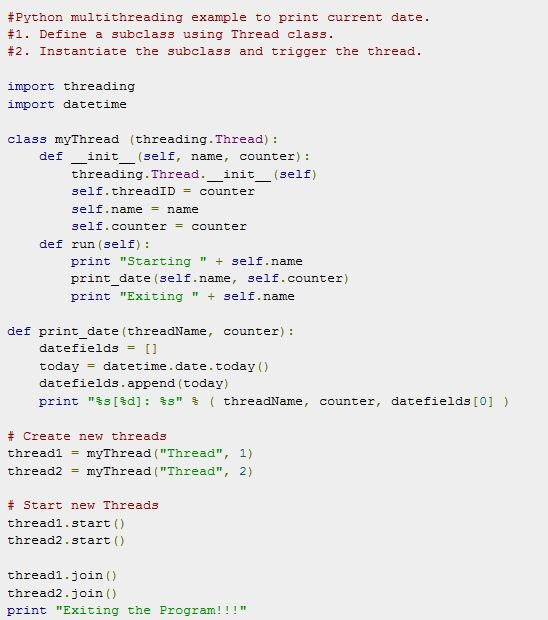
\includegraphics[width=0.75\textwidth]{figures/Thread}}
	\caption{Mengimplementasikan Thread menggunakan Threading}
	\label{Mengimplementasikan Thread menggunakan Threading}
\end{figure}

\chapter{XML Processing}
% Kelas D4 TI 3B Kelompok 3
% Diana Satima Gistivani 1154018
% M. Amran Hakim Siregar 1154106
% Indah Rahmawati 1154070
% Rizky Abdul Ghani Suherli 1154058


\section{Python XML Processing}
  XML adalah bahasa open source portable yang mungkinkan pemrogram mengemangkan aplikasi yang dapat dibaca oleh aplikasi lain, bahasa markup untuk keperluan umum yang disarankan oleh W3C untuk membuat dokumen markup keperluan pertukaran data antar sistem yang beraneka ragam. XML merupakan kelanjutan dari HTML (HyperText Markup Language) yang merupakan bahasa standar untuk melacak Internet.
terlepas dari sistem operasi dan bahasa pengembangnya .
\subsection{Apa itu XML}
  Extensible Markup Languange (XML) adalah bahasa markup seperti HTML atau SGML. 
Ini direkomendasikan oleh World Wide Web Consortium dan tersedia sebagai standar terbuka.
XML sangat berguna untuk mencatat data berukuran kecil dan menengah tanpa memerlukan tulang punggung berbasis SQL  
Pada kenyataanya dalam dunia komputer, sistem komputer dan database mengandung data yang tidak kompatibel satu sama lain. Dengan demikian tidak mungkin terjadinya pertukaran data melalui internet jika terdapat perbedaan sistem operasi dan aplikasi database yang digunakan.
Dengan menggunakan XML untuk pertukaran data, masalah perbedaan platform dan aplikasi tidak perlu diresahkan lagi. karena data yang disimpan pada XML dapat dibaca oleh berbagai macam platform dan aplikasi.

\subsection{Keunggulan dan Kelemahan Python XML Processing}
\subsubsection{Keunggulan Python XML Processing}
\begin{enumerate}
Keunggulan dari python dapat dijabarkan dari faktor-faktor berikut ini :
\item Quality : Python merupakan piranti lunak yang memakai meodologi reusability sehingga komponen-komponen pembangun piranti      lunak mudah digunakan dan diatur.
\item Productivity : penulisan program menggunakan python lebih mudah, karena interpreter menangani source code secara terpisah pada lower-level language.Interpreter menangani tipe deklarasi variabel,manajemen memory dan source code.
\item Portability : program python dapat dieksekusi di berbagai jenis komputer.Dengan demikian proses eksekusi program dapat dilakukan tanpa mengubah source code program.
\item Integration : phyton dirancang untuk dapat berinteraksi dengan aplikasi lain.Dengan demikian,program yang dibangun dengan bahasa pemrograman lain dapat dieksekusi dengan mudah padascript phyton dengan menggunakan function bahasa pemrograman lainnya.
\item Tidak ada tahapan kompilasi dan penyambungan (link) sehingga kecepatan perubahan pada masa pembuatan sistem aplikasi meningkat.
\item Tidak ada deklarasi tipe data yang merumitkan sehingga program menjadi lebih sederhana, singkat, dan fleksible.
\item Manajemen memori otomatis yaitu kumpulan sampah memori sehingga dapat menghindari pencacatan kode.
\item Tipe data dan operasi tingkat tinggi yaitu kecepatan pembuatan sistem aplikasi menggunakan tipe objek yang telah ada.
\item Pemrograman berorientasi objek.
\item Pelekatan dan perluasan dalam C.
\item Terdapat kelas, modul, eksepsi sehingga terdapat dukungan pemrograman skala besar secara modular.
\item Pemuatan dinamis modul C sehingga ekstensi menjadi sederhana dan berkas biner yang kecil
\item Pemuatan kembali secara dinamis modul phyton seperti memodifikasi aplikasi tanpa menghentikannya.
\item Model objek universal kelas Satu.
\item Konstruksi pada saat aplikasi berjalan.
\item Interaktif, dinamis dan alamiah.
\item Akses hingga informasi interpreter.
\item Portabilitas secara luas seperti pemrograman antar platform tanpa ports.
\item Kompilasi untuk portable kode byte sehingga kecepatan eksekusi bertambah dan melindungi kode sumber.
\item Antarmuka terpasang untuk pelayanan keluar seperti perangkat Bantu system, GUI, persistence, database, dll.


\end{enumerate}
 
\subsection {Arsitektur XML dan API}
  Perpustakaan standar Python menyediakan seperangkat antarmuka minimal tapi berguna untuk bekerja dengan XML. Dua API yang paling dasar dan umum digunakan untuk data XML adalah antarmuka SAX dan DOM. 
\subsubsection {System Arsitektur XML}
\begin{enumerate}
Sistem terdiri dari 3 lapisan yaitu :
\item lapisan database :Lapisan ini digunakan untuk menyimpan dokumen XML.Dalam system ini digunakan DBMS SQL Server.SQL
Server mengenalkan tipe data XML.Tipe data ini dapat digunakan dalam definisi tabel untuk mendefinisikan tipe sebuah kolom, tipe variabel dalam kode prosedural Transact-SQL, dan sebagai parameter prosedur.
\item lapisan bahasa query : XML, seperti basisdata relasional, mempunyai bahasa query sendiri yang dioptimasi untuk format data.Berpasangan dengan tipe data xml, hal ini mempercepat dan mengefisienkan penyimpanan dan temukembali data XML.
\item lapisan aplikasi : Lapisan ini merupakan antarmuka menggunakan bahasa Indonesia. Bahasa pemrograman yang digunakan adalah Java.Java menyediakan banyak fasilitas yang memudahkan untuk mengimplementasikan system yang dibuat.

\subsubsection {SAX}
  API sederhana untuk XML (SAX): mendaftarkan panggilan kemali untuk acara yang diminati dan kemudian membiarkan parser berjalan melalui dokumen. Ini berguna bila dokumen berukuran besar atau memiliki keterbatasan memori, ini memparsing file tidak pernah tersimpan dalam memori. Biasanya juga SAX ini dapat di pakai oleh Generator untuk membaca file XML dan pesan SAX ini juga biasa disebut dengan istilah event. SAX akan di kirimkan oleh Generator ke pipeline. SAX atau event ini juga dapat mengirimkan sebuah dokumen atau lampiran yang artinya SAX atau event ini dapat di proses nantinya.
  
\subsubsection {DOM}
  API Document Objek Model (DOM): ini adalah rekomendasi World Wide Web Consortium dimana keseluruhan file dibaca ke memori dan disimpan dalam bentuk hierarkies (tree-based) untuk mewakili semua fitur dokumen XML. 

SAX jelas tidak bisa memproses informasi secepat DOM saat bisa bekerjadengan file besar. Di sisi lain, menggunakan DOM secara eklusifenar-benar dapat membunuh sumber daya, terutama jika digunakan pada banyak file kecil. SAX hanya bisa dibaca sementara DOM mengizinkan perubahan pada file XML. Kedua API yang berbeda ini saling melengkapi satu sama lain, tidak ada alasan mengapa tidak dapat menggunakannya untuk proyek besar. 

Contoh: 
\begin{verbatim}
<collection shelf="New Arrivals"> 
<movie title="Enemy Behind"> 
  <type>War, Thriller</type> 
  <format>DVD</format> 
  <year>2003</year> 
  <rating>PG</rating> 
  <stars>10</stars>
  <description>Talk about a US-Japan war</description> 
</movie> 
<movie title="Transformers"> 
  <type>Anime, Science Fiction</type> 
  <format>DVD</format> 
  <year>1989</year> 
  <rating>R</rating> 
  <stars>8</stars> 
  <description>A schientific fiction</description> 
</movie> 
  <movie title="Trigun"> 
  <type>Anime, Action</type> 
  <format>DVD</format> 
  <episodes>4</episodes>  
  <rating>PG</rating> 
  <stars>10</stars> 
  <description>Vash the Stampede!</description> 
</movie>
<movie title="Ishtar"> 
  <type>Comedy</type> 
  <format>VHS</format> 
  <rating>PG</rating> 
  <stars>2</stars> 
  <description>Viewable boredom</description> 
</movie> 
</collection> 
\end{verbatim}


\subsection{Parsing XML dengan API SAX}
  SAX adalah antarmuka standar untuk parsing XML berbasis event. Parsing XML dengan SAX umumnya mengharuskan untuk membuat dengan subclassing xml.sax.
  ControlHandler menangani tag dan atribut tertentu dari XML. Objek ControlHandler menyediakan metode untuk menangani berbagai aktivitas parsing. Parsing memanggil metode ControlHandler saat memparsing file XML.
  Metode startDocument dan endDocument disebut awal dan akhir setiap elemen. Jika parsing tidak dalam mode namespace, metode startElement (tag attribute) dan endElement (tag) dipanggil. Jika tidak, metode yang sesuai startElemenNS dan endElemenNS dipanggil. 

Berikut ini metode penting untuk memahami sebelum melanjutkan ke materi berikutnya : 
\begin{enumerate}
  \item Metode berikut membuat objek parsing baru dan mengembalikannya. Objek parsing diuat akan menjadi tipe parsing pertama yang ditemukan sistem.
  \item xml.sax.make parser([parser list])
\end{enumerate}

Berikut adalah detail parameternya : 
\begin{enumerate}
  \item Parser list : pilihan argumen yang terdiri dari daftar parsing untuk digunakan yang semuanya harus menerapkan metode {make    parse}.
  \item Metode berikut membuat parsing SAX dan menggunakannya untuk mengurai dokumen. xml.sax.parser(xmlfile, contenthandler[, errorhandler])
\end{enumerate}

Membuat parsing SAX dan mengurai string XML yang ditentukan : 
xml.sax.parsertring(xmlstring,contenthandler[, errorhandler])

Brikut ini adalah detail nama dari parameter : 
\begin{enumerate}
  \item  {XMLstring}  = Nama dari string yang bisa dibaca.
  \item  {ContentHandler} = Menjadi objek ContenHandler.
  \item  {ErrorHandler} = Menjadi objek ErorHandler SAX. 
\end{enumerate}

Contoh : 
\begin{verbatim}
  \#  
  /usr/bin/python
import xml.sax 
class MovieHandler( xml.sax.ContentHandler ): 
~~ def init (self): 
~~~~~ self.CurrentData = "" 
~~~~~ self.type = "" 
~~~~~ self.format = "" 
~~~~~ self.year = "" 
~~~~~ self.rating = "" 
~~~~~ self.stars = "" 
~~~~~ self.description = "" 
~~ \#  Call when an element starts 
~~ def startElement(self, tag, attributes):
~~~~~ self.CurrentData = tag 
~~~~~ if tag == "movie": 
~~~~~~~~ print "*****Movie*****" 
~~~~~~~~ title = attributes["title"] 
~~~~~~~~ print "Title:", title 
~~ \#  Call when an elements ends 
~~ def endElement(self, tag): 
~~~~~ if self.CurrentData == "type":
~~~~~~~~ print "Type:", self.type 
~~~~~ elif self.CurrentData == "format": 
~~~~~~~~ print "Format:", self.format 
~~~~~ elif self.CurrentData == "year": 
~~~~~~~~ print "Year:", self.year 
~~~~~ elif self.CurrentData == "rating": 
~~~~~~~~ print "Rating:", self.rating 
~~~~~ elif self.CurrentData == "stars": 
~~~~~~~~ print "Stars:", self.stars 
~~~~~ elif self.CurrentData == "description": 
~~~~~~~~ print "Description:", self.description 
~~~~~ self.CurrentData = "" 
~~ \#  Call when a character is read 
~~ def characters(self, content): 
~~~~~ if self.CurrentData == "type":
~~~~~~~~ self.type = content 
~~~~~ elif self.CurrentData == "format": 
~~~~~~~~ self.format = content 
~~~~~ elif self.CurrentData == "year": 
~~~~~~~~ self.year = content 
~~~~~ elif self.CurrentData == "rating": 
~~~~~~~~ self.rating = content 
~~~~~ elif self.CurrentData == "stars":
~~~~~~~~ self.stars = content 
~~~~~ elif self.CurrentData == "description": 
~~~~~~~~ self.description = content 
if (name  == " main "): 
~~ \#  create an XMLReader 
~~ parser = xml.sax.make parser() 
~~ \#  turn off namepsaces
~~ parser.setFeature(xml.sax.handler.feature namespaces, 0) 
~~ \#  override the default ContextHandler 
~~ Handler = MovieHandler() 
~~ parser.setContentHandler( Handler )
~~ parser.parse("movies.xml") 
\end{verbatim}

Ini akan menghasilkan hasil sebagai berikut: 
\begin{verbatim}
{*****Movie******} 
{*****Movie*****} 
{Title: Enemy Behind} 
{Type: War, Thriller} 
{Format: DVD} 
{Year: 2003} 
{Rating: PG} 
{Stars: 10} 
{Description: Talk about a US-Japan war}
{*****Movie*****} 
{Title: Transformers} 
{Type: Anime, Science Fiction}
{Format: DVD} 
{Year: 1989} 
{Rating: R}
{Stars: 8} 
{Description: A schientific fiction} 
{*****Movie*****} 
{Title: Trigun} 
{Type: Anime, Action} 
{Format: DVD}
{Rating: PG} 
{Stars: 10} 
{Description: Vash the Stampede!} 
{*****Movie*****} 
{Title: Ishtar}
{Type: Comedy} 
{Format: VHS}
{Rating: PG} 
{Stars: 2} 
\end{verbatim}

\subsection{2.3 Parsing XML dengan API DOM} 
Document Ovject Model (DOM) adalah API lintas bahasa dari World Wide Web Consortium (W3C) untuk mengakses dan memodifikasi dokumen XML.  DOM sangat berguna untuk aplikasi akses acak. SAX hanya memungkinkan melihat satu bit dokumen sekaligus. Jika melihat satu elemen SAX, tidak memiliki akses ke yang lain. Berikut adalah cara termudah untuk memuat dokumen XML dengan cepat dan membuat objek minidom menggunakan modul xml.dom. Objek minidom menyediakan metode parsing sederhana yang dengan cepat memuat pohon DOM dari file XML. \par
Contoh~frase memanggil fungsi  parsing (file [,parsing]) dari objek minidokumen untuk mengurai file XML yang ditunjuk oleh file ke objek pohon DOM.
\begin{enumerate}
\item $  \#  $!/usr/bin/python
from xml.dom.minidom import parse 
import xml.dom.minidom 
\item $  \#  $ Open XML document using minidom parser
DOMTree = xml.dom.minidom.parse("movies.xml") 
collection = DOMTree.documentElement 
if collection.hasAttribute("shelf"): 
print "Root element :  $  \%  $s"  $  \%  $ collection.getAttribute("shelf") 
\item $  \#  $ Get all the movies in the collection 
movies = collection.getElementsByTagName("movie") 
\item $  \#  $ Print detail of each movie. 
for movie in movies: 
print "*****Movie*****" 
if movie.hasAttribute("title"): 
print "Title:  $  \%  $s"  $  \%  $ movie.getAttribute("title") 
type = movie.getElementsByTagName('type')[0] 
print "Type:  $  \%  $s"  $  \%  $ type.childNodes[0].data 
format = movie.getElementsByTagName('format')[0] 
print "Format:  $  \%  $s"  $  \%  $ format.childNodes[0].data 
rating = movie.getElementsByTagName('rating')[0] 
print "Rating:  $  \%  $s"  $  \%  $ rating.childNodes[0].data 
description = movie.getElementsByTagName('description')[0] 
print "Description:  $  \%  $s"  $  \%  $ description.childNodes[0].data 
Ini akan menghasilkan hasil sebagai berikut : 
Root element : New Arrivals 
*****Movie***** 
Title: Enemy Behind 
Type: War, Thriller 
Format: DVD 
Rating: PG 
Description: Talk about a US-Japan war 
*****Movie***** 
Title: Transformers 
Type: Anime, Science Fiction 
Format: DVD 
Rating: R 
Description: A schientific fiction 
*****Movie***** 
Title: Trigun 
Type: Anime, Action 
Format: DVD 
Rating: PG 
Description: Vash the Stampede! 
*****Movie***** 
Title: Ishtar 
Type: Comedy 
Format: VHS 
Rating: PG
Description: Viewable boredom 
\end{enumerate}

\subsection{Membangun Parsing Document XML menggunakan Python} 
Python mendukung untuk bekerja dengan berbagai bentuk markup data terstruktur. Selain mengurai xml.etree. \textit{ElementTree} mendukung pembuatan dokumen XML yang terbentuk dengan baik dari objek elemen yang dibangun dalam aplikasi. Kelas elemen digunakakan saat sebuah dokumen diurai untuk mengetahui bagaimana menghasilkan bentuk serial dari isinya kemudian dapat ditulis ke sebuah file.  
Untuk membuat instance elemeb gunakan fungsi elemen contructor dan \textit{SubElemen()} pabrik. 
Import xml.etree.ElementTree as xml \par
\vspace{12pt}
\noindent 
{\fontsize{10pt}{10pt}\selectfont filename =  $ " $/home/abc/Desktop/test $  \_  $xml.xml $ " $} \par
\noindent 
{\fontsize{10pt}{10pt}\selectfont toot = xml.Element( $ " $Users $ " $)} \par
\noindent 
{\fontsize{10pt}{10pt}\selectfont userelement = xml.Element( $ " $user $ " $)} \par
\noindent 
{\fontsize{10pt}{10pt}\selectfont root.append(userelement)} \par
\noindent 
\vspace{10pt}
\noindent 
Bila menjalankan ini, akan menghasilkan sebagai berikut : \par
\noindent 
{\fontsize{10pt}{10pt}\selectfont <Users>} \par
\noindent 
{\fontsize{10pt}{10pt}\selectfont  \hspace*{0.5in} <user>} \par
\noindent 
{\fontsize{10pt}{10pt}\selectfont  \hspace*{0.5in} <user>} \par
\noindent 
{\fontsize{10pt}{10pt}\selectfont </Users>} \par
\vspace{10pt}
\vspace{10pt}
\vspace{10pt}
\noindent 
Tambahkan anak-anak pegguna \par
\vspace{10pt}
\noindent 
{\fontsize{10pt}{10pt}\selectfont Uid = xml.SubElement(userelement,  $ " $uid $ " $)} \par
\noindent 
{\fontsize{10pt}{10pt}\selectfont Uid.text =  $ " $1 $ " $} \par
\vspace{10pt}
\noindent 
{\fontsize{10pt}{10pt}\selectfont FirstName = xml.SubElement(userelement,  $ " $FirstName $ " $)} \par
\noindent 
{\fontsize{10pt}{10pt}\selectfont FirstName.text =  $ " $testuser $ " $} \par
\vspace{10pt}
\noindent 
{\fontsize{10pt}{10pt}\selectfont LastName = xml.SubElement(userelement,  $ " $LastName $ " $} \par
\noindent 
{\fontsize{10pt}{10pt}\selectfont LastName.text =  $ " $testuser $ " $} \par
\vspace{10pt}
\noindent 
{\fontsize{10pt}{10pt}\selectfont Email = xml.SubElement(userelement,  $ " $Email $ " $)} \par
\noindent 
{\fontsize{10pt}{10pt}\selectfont Email.text = {mailto:testuser@test.com}{testuser@test.com}
} \par
\vspace{10pt}
\noindent 
{\fontsize{10pt}{10pt}\selectfont state = xml.SubElement(userelemet,  $ " $state $ " $)} \par
\noindent 
{\fontsize{10pt}{10pt}\selectfont state.text =  $ " $xyz $ " $} \par
\vspace{10pt}
\noindent 
{\fontsize{10pt}{10pt}\selectfont location = xml.SubElement(userelement,  $ " $location)} \par
\noindent 
{\fontsize{10pt}{10pt}\selectfont location.text = abc} \par
\vspace{10pt}
\noindent 
{\fontsize{10pt}{10pt}\selectfont tree = xml.ElementTree(root)} \par
\noindent 
{\fontsize{10pt}{10pt}\selectfont with open(filename,  $ " $w $ " $) as fh:} \par
\noindent 
{\fontsize{10pt}{10pt}\selectfont tree.write(fh)} \par
\vspace{10pt}
\noindent 
 \hspace*{0.5in} Pertama buat elemen root dengan mengunakan fungsi \textit{ElementTree}. Kemudian membuat elemen pegguna dan menambahkannya ke root. Selanjutnya membuat \textit{SubElement }dengan melewatkan elemen pengguna (userelement) ke \textit{SubElemen} beserta namanya seperto  $ " $FirstName $ " $. Kemudian untuk setiap \textit{SubElement} tetapkan properti teks untuk memberi nilai. Di akhir, membuat \textit{ElementTree} dan menggunakannya untuk menulis XML ke file. \par
\noindent 
 \hspace*{0.5in} Jika menjalankan ini akan menjadi sebagai berikut : \par
\noindent 
 {\fontsize{10pt}{10pt}\selectfont <users>} \par
\noindent 
{\fontsize{10pt}{10pt}\selectfont  \hspace*{0.5in} <user>} \par
\noindent 
{\fontsize{10pt}{10pt}\selectfont  \hspace*{0.5in}  \hspace*{0.5in} <uid>1</uid>} \par
\noindent 
{\fontsize{10pt}{10pt}\selectfont  \hspace*{0.5in}  \hspace*{0.5in} <FirstName>testuser</FirstName>} \par
\noindent 
{\fontsize{10pt}{10pt}\selectfont  \hspace*{0.5in}  \hspace*{0.5in} <LastName>testuser</LastName>} \par
\noindent 
{\fontsize{10pt}{10pt}\selectfont  \hspace*{0.5in}  \hspace*{0.5in} <state>xyz</state>} \par
\noindent 
{\fontsize{10pt}{10pt}\selectfont  \hspace*{0.5in}  \hspace*{0.5in} <location>abc</location>} \par
\noindent 
{\fontsize{10pt}{10pt}\selectfont  \hspace*{0.5in} </user>} \par
\noindent 
{\fontsize{10pt}{10pt}\selectfont </Users>} \par
\vspace{10pt}
\noindent 
Parsing XML Documen : \par
\vspace{12pt}
\noindent 
{\fontsize{10pt}{10pt}\selectfont import xml.etree.ElementTree as ET} \par
\noindent 
{\fontsize{10pt}{10pt}\selectfont tree = ET.parse(‘Your $  \_  $XML $  \_  $file $  \_  $path’)} \par
\noindent 
{\fontsize{10pt}{10pt}\selectfont root = tree.getroot()} \par
\noindent 
{\fontsize{10pt}{10pt}\selectfont 

 %%%%%%%%%%%%  Start New Page here %%%%%%%%%%%%%%


\newpage

}\vspace{10pt}
\vspace{10pt}
\noindent 
Disini \textit{getroot()} akan mengembalikan elemen dari dokumen XML \par
\vspace{10pt}
\noindent 
{\fontsize{10pt}{10pt}\selectfont <Users version= $ " $1.0 $ " $ languange= $ " $SPA $ " $>} \par
\noindent 
{\fontsize{10pt}{10pt}\selectfont  \hspace*{0.5in} <user>} \par
\noindent 
{\fontsize{10pt}{10pt}\selectfont  \hspace*{0.5in}  \hspace*{0.5in} <uid>1</uid>} \par
\noindent 
{\fontsize{10pt}{10pt}\selectfont  \hspace*{0.5in}  \hspace*{0.5in} <FirstName>testuser</FirstName>} \par
\noindent 
{\fontsize{10pt}{10pt}\selectfont  \hspace*{0.5in}  \hspace*{0.5in} <LastName>testuser</LastName>} \par
\noindent 
{\fontsize{10pt}{10pt}\selectfont  \hspace*{0.5in}  \hspace*{0.5in} <Email>testuser@tes.com/Email>} \par
\noindent 
{\fontsize{10pt}{10pt}\selectfont  \hspace*{0.5in}  \hspace*{0.5in} <state>xyz</state>} \par
\noindent 
{\fontsize{10pt}{10pt}\selectfont  \hspace*{0.5in}  \hspace*{0.5in} <location>abc</location>} \par
\noindent 
{\fontsize{10pt}{10pt}\selectfont  \hspace*{0.5in} </user>} \par
\noindent 
{\fontsize{10pt}{10pt}\selectfont </Users>} \par
\vspace{12pt}


\chapter{GUI Programming}
\documentclass [12pt,a4paper,notitlepage,oneside,bahasa]{article}
\usepackage[left=3.00 cm, right=2.00 cm, bottom=2.00 cm, top=3.00 cm]{geometry}
\begin{document}
\title{\textbf GUI Programming}
\maketitle

Python menyediakan berbagai pilihan untuk mengembangkan antarmuka pengguna grafis (GUIs). 
Berikut dibawah ini merupakan berbagai pilihan yang disediakan oleh Python :
\begin{itemize}
\item Tkinter \par
Tkinter merupakan standar bahasa python yang ditetapkan untuk membangun suatu antarmuka pengguna grafik (GUI). 
\item wxPython \par
wxPython adalah toolkit antarmuka pengguna grafis (GUI) yang digunakan dalam skripsi ini dan ini adalah pembungkus untuk toolkit wxWidgets.
\item Jpython \par
Port Python untuk java yang memberikan Python script akses tanpa batas ke perpustakaan kelas java pada mesin lokal \par
\end{itemize}
\vspace{12pt}
\noindent 
\section{\textbf Tkinter Pemrograman}
Tkinter adalah perpustakaan GUI standar untuk Python. Python bila dikombinasikan dengan Tkinter menyediakan cara yang amat mudah dan cepat untuk membuat aplikasi GUI. Tkinter menyediakan antarmuka yang berorientasi objek yang kuat untuk toolkit Tk GUI.
 \hspace*{0.5in} Membuat aplikasi GUI menggunakan Tkinter adalah tugas yang mudah. Yang diperlukan adalah melakukan langkah-langkah sebagai berikut : 
\begin{enumerate} 
	\item Mengimpor Tkinter modul 
	\item Buat jendela utama aplikasi GUI
	\item Tambahkan satu atau lebih dari widget tersebut diatas ke aplikasi GUI
	\item Masukkan acara loop utama untuk mengambil tindakan terhadap setiap peristiwa dipicu oleh pengguna
\end{enumerate}

 %%%%%%%%%%%%  Start New Page here %%%%%%%%%%%%%%


\newpage

\vspace{12pt}
\vspace{12pt}
\noindent 
Contoh : 
\begin{verbatim}
#!/usr/bin/python 
import Tkinter 
top = Tkinter.Tk()
# Code to add widgets will go here...
top.mainloop()
\end{verbatim}

\section{\textbf Tkinter Widget} \par
\noindent 
 \hspace*{0.5in} Tkinter menyediakan berbagai kontrol seperti tombol, label dan kotak teks yang digunakan dalam aplikasi GUI. 
 Kontrol ini biasanya disebut widget.
\noindent 
 \hspace*{0.5in} Saat ini ada 15 jenis widget di Tkinter. berikut adalah contoh widget serta penjelasan singkat pada tabel ini:


 %%%%%%%%%%%%  Table No:1 Here %%%%%%%%%%%%%%


\begin{table}[h]
	\caption{Ukuran}
		\begin{center}
		\begin{tabular}{|c|c|}
			\hline
			Operator & Penjelasan \\
			\hline
			Button & Menampilkan tombol dalam aplikasi\\
			Canvas & Menggambar bentuk seperti garis, oval, poligon dan persegi panjang dalam aplikasi\\
			Checkbutton & Menampilkan sejumlah pilihan sebagai kotak centang. Pengguna dapat memilih beberapa pilihan pada suatu waktu
			Entry & Menampilkan bidang garis teks tunggal untuk menerima nilai-nilai dari pengguna\\
			Frame & Wadah untuk mengatur widget lainnya\\
			Label & Memberikan keterangan garis single untuk widget lainnya. Hal ini berisi gambar\\
			Listbox & Menyediakan daftar pilihan kepada pengguna\\
			Menubutton & Menampilkan menu dalam aplikasi\\
			Menu & Memberikan berbagai perintah untuk pengguna. Perintah-perintah ini terkandung di dalam MenuButton\\
			Message & Menampilkan bidang teks multiline untuk menerima nilai-nilai dari pengguna\\
			RadioButton & Menampilkan sejumah pilihan sebagai tombol radio. Pengguna dapat memilih hanya satu pilihan pada suatu waktu\\
			Scale & Menyediakan widget slide\\
			Scrollbar & Menambah kemampuan bergulir ke berbagai widget seperti kotak daftar\\
			Text & Menampilka teks dalam beberapa garis\\
			Toplevel & Menyediakan wajah jendela terpisah\\
			PanedWindow & Wadah yang mengandung sejumlah panel disusun horizontal atau vertikal\\
			LabelFrame & Wadah widget sederhana. Bertindak sebagai spacer atau wajah untuk layout jendela kompleks\\
			TkMessageBox & Menampilkan kotak pesan dalam aplikasi\\
			Spinbox & Memilih sejumlah tetap nilai-nilai&\\
		\hline
		\end{tabular}
		\end{center}
	\begin{tablenotes}
	\end{tablenotes}
\end{table}

	


 %%%%%%%%%%%%  Table No:1 Ends Here %%%%%%%%%%%%%%


\vspace{12pt}
subsection{Atribut Tkinter}
\noindent 
 \hspace*{0.5in} Beberapa atribut umum sebagai ukuran, warna dan font ditentukan. Berikut adalah beberapa atribut standar :
\noindent 
\begin{enumerate}
\item Ukuran 
Berbagai panjang, lebar, dan dimensi lain dari widget digambarkan dalam banyak unit yang berbeda seperti 
\item Jika menetapkan dimensi ke integer diasumsikan dalam piksel 
\item Menentukan unit dengan menentukan dimensi untuk string yang berisi sejumlah diikuti oleh :
\end{itemize}
 


 %%%%%%%%%%%%  Table No:2 Here %%%%%%%%%%%%%%


\begin{table}[ht]
	\caption{Ukuran}
	\bein{center}
	\begin{tabular}{|c|c|}
		\hline
		Karakter&  Penjelasan \cr
		\hline
		c&Sentimeter\\
		i&Inci\\
		m&Milimeter\\
		p&Poin printer\\
		\hline
	\end{tabular}
	\end{center}
	\begin{tablenotes}
	\end{tablenotes}
\end{table}


 %%%%%%%%%%%%  Table No:2 Ends Here %%%%%%%%%%%%%%

 
 \hspace*{0.5in} \vspace{12pt}
 subsection{Panjang Tkinter}
 \hspace*{0.5in} Tkinter mengungkapkan panjang sebagai integer jumlah piksel. Berikut ini adalah daftar pilihan panjang umum:
\noindent 
\begin{itemize}
	\item borderwidth
	Lebar batas yang memberikan tampilan tiga dimensi untuk widget
	\item highlightthickness
	Lebar puncak persegi panjang ketika widget memiliki fokus
 	\item padX padY
	Ruang tambahan widget dari manajer tata letak luar minimum widget perlu menampilkan isinya di x dan y arah
	\item selectborderwidth
	Lebar perbatasan tiga dimensi disekitar dipilih item widget
	\item wraplength \par
	Panjang garis maksimum untuk widget yang melakukan kata membungkus
	\item height
	Tinggi diinginkan widget
	\item underline
	Indeks karakter untuk menggarisawahi dalam teks widget 
	\item width
	\item Lebar diinginkan widget
\end{itemize}
 
\noindent 
subsection{Warna Tkinter}
\noindent 
Tkinter memiliki warna dengan string. Ada dua cara umum untuk menentukan sebuah warna di Tkiter, yaitu : \par
\noindent 
\begin{itemize}
	\item Menggunakan string menentukan proporsi merah, hijau dan biru didigit heksadesimal. Misalnya  `` \#ffff '' putih,  ``  \#000000 '' hitam dan  ``\#000fff000 '' hijau.
\noindent 
	\item Menggunakan lokal standar nama warna . warna-warna ``white'', ``black'',  ``green'' dan  ``magenta'' akan selalu tersedia.
\end{itemize}

\vspace{12pt}
Pilihan warna umum :
\noindent 
\begin{itemize}
	\item activebackground \par
	Warna latar berlakang untuk widget ketika widget aktif \par
	\noindent 
	\item activeforeground \par
	Warna depan untuk widget ketika widget aktif \par
	\noindent 
	\item background \par
	Merepresentasikan sebagai \textit{bg} \par
	\noindent 
	\item disableforeground \par
	Warna depan untuk widget ketika widget dinonaktifkan \par
	\noindent 
	\item foreground \par
	Merepresentasikan fg \par
	\noindent 
	\item highlightbackground \par
	Warna latar belakang dari daerah puncak ketika widget memiliki fokus \par
	\noindent 
	\item hightlightcolor \par
	Warna depan dari wilayah puncak ketika widget memiliki fokus \par
	\noindent 
	\item selectbackground \par
	Warna latar belakang untuk item yang dipilih dari widget \par
	\noindent 
	\item selectforeground \par
	Warna depan untuk item yang dipilih dari widget \par
	\noindent 
	\item Font \par
	\noindent 
	Sebagai tupel yang elemen pertama adalah keluarga font diikuti dengan string yang berisi satu atau lebih gaya pengubah tebal,miring, garis bawah dan overstrike. 
	end{itemize}
	\noindent 
Contoh : \par
	\begin{itemize}
		\noindent
		\item ( ``Helvetica'', ``16 '') untuk 16 \- point Helvetica biasa \par
		\noindent 
		\item ( ``Times'', ``24 '',``beranimiring'') untuk 24 \- point kali miring tebal
	\end{itemize}
 		\par
\vspace{12pt}
Dapat membuat  ``font object'' dengan mengimpor modul tkFont dan menggunakan kelas konstruktor font nya : \par
Import tkFont \par
Font = tkFont.Font (option, ....) \par
\vspace{12pt}
Berikut adalah daftar pilihan : \par
\noindent 
\begin{itemize}
	\item Family \par
	Font nama keluarga sebagai string \par
	\noindent 
	\item Size \par
	Font tinggi sebagai integer dalam poin \par
	\noindent 
	\item Weight \par
	Bold untuk teal, normal untuk berat badan secara teratur \par
	\noindent 
	\item Slant \par
	Italic untuk miring, roman untuk unstlanted \par
	\noindent 
	\item Underline \par
	1 untuk teks yang digarisbawahi, 0 untuk normal \par
	\noindent 
	\item Overstrike \par
	1 untuk teks telak, 0 untuk normal \par
	Jika berjalan di bawah X window system, dapat menggunakan salah satu nama font X. Sebagai contoh, font bernama  \verb|"-*lucidatypewriter-medium-r-*-*-*-140-*-*-*"| adalah favorit fixed-width font penulis untuk digunakan pada layar. \par
	\noindent 
	\item Jangkar \par
	\noindent 
	Jangkar digunakan untuk mendefinisikan mana teks diposisikan relatif terhadap titik acuan. Berikut adalah daftar kemungkinan konstanta yang dapat digunakan :
	\noindent
	\begin{itemize}
		\item NW  
		\item N
		\item NE
		\item W
		\item TENGAH
		\item E
		\item SW
		\item S
		\item SE
	\end{itemize}
\end{itemize}
 \par
\vspace{12pt}
Jika menggunakan tengah sebagai jangkar tek, tek akan ditengahkan horizontal dan vertikal disekitar titik referensi. \par
Jangkar NW akan posisi teks sehingga titik referensi bertepatan dengan laut sudut kotak berisi teks \par
Jangakr W akan pusat teks secara vertikal disekitar satu titik referensi dengan tepi kiri kotak teks yang melewati titik itu dan sebagainya. \par
Jika membuat widget kecil didalam bingkai besar dan menggunakan jangkar = SE pilihan, widget akan ditempatkan disudut kanan bawah gambar. Jika menggunakan anchor = N sebaliknya widget akan dipusatkan disepanjang tepi atas. \par
\noindent 

subsection{Gaya relief}

Widget mengacu pada efek 3-D simulasi terbaru disekitar bagian luar widget. Berikut adalah daftar konstanta yang mungkin dapat digunakan untuk atribut:
\begin{itemize}
	\item Datar
	\item Dibesarkan
	\item Cekung
	\item Alur
	\item Punggung bukit
\end{itemize}


\vspace{12pt}
Contoh : \par
{\fontsize{10pt}{10pt}\selectfont From Tkinter import *} \par
{\fontsize{10pt}{10pt}\selectfont Import Tkinter} \par
\vspace{10pt}
{\fontsize{10pt}{10pt}\selectfont top = Tkinter.Tk()} \par
{\fontsize{10pt}{10pt}\selectfont B1 = Tkinter.Button(top, text= $ " $FLAT $ " $, relief=FLAT)} \par
{\fontsize{10pt}{10pt}\selectfont B2 = Tkinter.Button(top, text= $ " $RAISED $ " $, relief=RAISED)} \par
{\fontsize{10pt}{10pt}\selectfont B3 =Tkinter.Button(top, text= $ " $SUNKEN $ " $, relief=SUNKEN)} \par
{\fontsize{10pt}{10pt}\selectfont B4=Tkinter.Button(top, text= $ " $GROOVE $ " $, relief=GROOVE)} \par
{\fontsize{10pt}{10pt}\selectfont B5=Tkinter.Button(top, text= $ " $RIDGE $ " $, relief=RIDGE)} \par
\vspace{10pt}
{\fontsize{10pt}{10pt}\selectfont B1.pack()} \par
{\fontsize{10pt}{10pt}\selectfont B2.pack()} \par
{\fontsize{10pt}{10pt}\selectfont B3.pack()} \par
{\fontsize{10pt}{10pt}\selectfont B4.pack()} \par
{\fontsize{10pt}{10pt}\selectfont B5.pack()} \par
{\fontsize{10pt}{10pt}\selectfont top.mainloop()} \par
\noindent 
Britmaps \par
\noindent 
Ada beberapa jenis bitmap yang tersedia, diantaranya: \par
\noindent 
\begin{itemize}
\item Kesalahan \par
\noindent 
\item Gray75 \par
\noindent 
\item Gray50 \par
\noindent 
\item Gray12 \par
\noindent 
\item Jam Pasir \par
\noindent 
\item Info \par
\noindent 
\item Questhead \par
\noindent 
\item Perantanyaan  \par
\noindent 
\item Peringatan\end{itemize}
 \par
\vspace{12pt}
Contoh: \par
{\fontsize{10pt}{10pt}\selectfont From Tkinter import *} \par
{\fontsize{10pt}{10pt}\selectfont Import Tkinter} \par
\vspace{10pt}
{\fontsize{10pt}{10pt}\selectfont Top = Tkinter.Tk()} \par
\vspace{10pt}
{\fontsize{10pt}{10pt}\selectfont B1 = Tkinter.Button(top, text = $ " $error $ " $, relief=RAISED,  $  \setminus  $ bitmap= $ " $error $ " $)} \par
{\fontsize{10pt}{10pt}\selectfont B2 = Tkinter.Button(top, text = $ " $hourglass $ " $, relief=RAISED,  $  \setminus  $ bitmap= $ " $hourglass $ " $)} \par
{\fontsize{10pt}{10pt}\selectfont B3 = Tkinter.Button(top, text = $ " $info $ " $, relief=RAISED,  $  \setminus  $ bitmap= $ " $info $ " $)} \par
{\fontsize{10pt}{10pt}\selectfont B4 = Tkinter.Button(top, text = $ " $question $ " $, relief=RAISED,  $  \setminus  $ bitmap= $ " $question $ " $)} \par
{\fontsize{10pt}{10pt}\selectfont B5 = Tkinter.Button(top, text = $ " $warning $ " $, relief=RAISED,  $  \setminus  $ bitmap= $ " $warning $ " $)} \par
\vspace{10pt}
{\fontsize{10pt}{10pt}\selectfont B1.pack()} \par
{\fontsize{10pt}{10pt}\selectfont B2.pack()} \par
{\fontsize{10pt}{10pt}\selectfont B3.pack()} \par
{\fontsize{10pt}{10pt}\selectfont B4.pack()} \par
{\fontsize{10pt}{10pt}\selectfont B5.pack()} \par
{\fontsize{10pt}{10pt}\selectfont top.mainloop()} \par
\noindent 
Kursor \par
\noindent 
Berikut daftar menarik : \par
\noindent 
\begin{itemize}
\item Panah \par
\noindent 
\item Lingkaran \par
\noindent 
\item Jam \par
\noindent 
\item Menyebrang \par
\noindent 
\item Dotbox \par
\noindent 
\item Bertukar \par
\noindent 
\item Fluer \par
\noindent 
\item Jantung \par
\noindent 
\item Manusia \par
\noindent 
\item Tikus \par
\noindent 
\item Bajak laut \par
\noindent 
\item Tamah \par
\noindent 
\item Antar jemput \par
\noindent 
\item Perekat \par
\noindent 
\item Laba-laba \par
\noindent 
\item Kaleng semprot \par
\noindent 
\item Bintang \par
\noindent 
\item Target \par
\noindent 
\item Tcross \par
\noindent 
\item Melakukan perjalanan \par
\noindent 
\item Menonton\end{itemize}
 \par
\vspace{12pt}
Contoh : \par
{\fontsize{10pt}{10pt}\selectfont From Tkinter import *} \par
{\fontsize{10pt}{10pt}\selectfont Import Tkinter} \par
\vspace{10pt}
{\fontsize{10pt}{10pt}\selectfont Top = Tkinter.Tk()} \par
\vspace{10pt}
{\fontsize{10pt}{10pt}\selectfont B1 = Tkinter.Button(top, text = $ " $circle $ " $, relief=RAISED,  $  \setminus  $ bitmap= $ " $circle $ " $)} \par
{\fontsize{10pt}{10pt}\selectfont B2 = Tkinter.Button(top, text = $ " $plus $ " $, relief=RAISED,  $  \setminus  $ bitmap= $ " $plus $ " $)} \par
\vspace{10pt}
{\fontsize{10pt}{10pt}\selectfont B1.pack()} \par
{\fontsize{10pt}{10pt}\selectfont B2.pack()} \par
{\fontsize{10pt}{10pt}\selectfont top.mainloop()} \par
\vspace{10pt}
\noindent 
\textbf{3.3 Manajemen Geometri} \par
\noindent 
 \hspace*{0.5in} Semua widget tkinter memiliki akses ke metode manajemen geometri tertentu, yang memiliki tujuan menggorganisir widget diseluruh wilayah widget induk. Tkinter mengekspos kelas manager geometri berikut : \par
\noindent 
\begin{itemize}
\item Metode the \textit{pack()} \par
\noindent 
Manajer geometri ini mengatur widget diblok sebelum menempatkan mereka di widget induk \par
\noindent 
\item Metode the \textit{grid()} \par
\noindent 
Manajer geometri ini mengatur widget dalam struktur tabel seperti di widget induk \par
\noindent 
\item Metode the  \textit{place()}\end{itemize} \par
\noindent 
Manajer geometri ini mengatur widget dengan menempatkan dalam posisi tertentu dalam widget induk \par
\vspace{12pt}
\noindent 
\textbf{3.4 Manfaat Tkinter} \par
Tkinter sangat sederhana. Berikut manfaat Tkinter dibandingkan GUI toolkit : \par
\noindent 
\begin{itemize}
\item 
Tkinter terdiri dari sejumlah modul.  (Tkinter)\vspace{\baselineskip}
Antarmuka Tk terletak di modul biner
bernama _tkinter (ini adalah tkinter di versi sebelumnya). Modul ini berisi lowlevel
antarmuka ke Tk, dan tidak boleh digunakan langsung oleh pemrogram aplikasi. ini
biasanya shared library (atau DLL), tapi mungkin dalam beberapa kasus secara statis terkait dengan
Penerjemah Python. \par
\noindent
\item Tkinter mudah diakses oleh siapa saja. (Accessibilty)\vspace{\baselineskip}
Tkinter merupakan toolkit yang ringan dan satu-satunya solusi GUI yang paling sederhana untuk Python sampai saat ini. Cukup menuliskan 
beberapa baris kode Python untuk membuat aplikasi GUI sederhana dengan Tkinter. Untuk menambahkan komponen baru pada Tkinter, dapat 
membuatnya dalam kode Python atau menambahkan paket ekstensi seperti Pmw, Tix, atau ttk. \par
\noindent 
\item widget root tk (widget root tk)\vspace{\baselineskip}
Untuk menginisialisasi Tkinter, kita harus membuat widget root Tk. Ini adalah jendela biasa, dengan
judul bar dan hiasan lainnya yang disediakan oleh window manager Anda. Anda seharusnya saja
buat satu widget root untuk setiap program, dan itu harus dibuat sebelum widget lainnya. \par
\noindent 
\item Tkinter mudah digunakan di semua platform (Portability)\vspace{\baselineskip}
Sebuah program Python yang dibangun menggunakan Tkinter dapat berjalan dengan baik di semua platform sistem operasi seperti Microsoft 
Windows, Linux, dan Macintosh. Dan dari segi tampilan window, akan terlihat sama dengan standar platform yang digunakan. \par
\noindent 
\item Tkinter selalu tersedia di Python (Availability)\vspace{\baselineskip}
Tkinter merupakan modul standar pada pustaka Python. Sebagian besar paket instalasi Python sudah langsung berisi Tkinter. Khusus untuk 
beberapa distro Linux, perlu menambahkan paket Tkinter secara terpisah. Pada Windows, bisa langsung menggunakan Tkinter sesaat setelah 
menginstal paket instalasi Python. \par
\noindent 
\item handles bagus di gunakan di Python (Handles)\vspace{\baselineskip}
item kandles merupakan nilai integer yang digunakan untuk mengidentifikasi item tertentu pada kanvas. Tkinter secara otomatis menugaskan 
pegangan baru ke setiap item baru yang dibuat di atas kanvas. Item Handles dapat di lewatkan ke berbagai metode kanvas baik sebagai 
bilangan bulat atau sebagai string. Tag adalah nama simbolis yang dilekatkan pada item. Tag adalah string biasa, dan bisa berisi apa 
saja kecuali spasi (asalkan tidak sesuai dengan item pegangan). \par
\noindent 
\item Modul Tkinter menyediakan kelas yang sesuai dengan berbagai jenis widget di Tk (Module)\vspace{\baselineskip}
dan sejumlah mixin dan kelas pembantu lainnya (mixin adalah kelas yang dirancang untuk menjadi
dikombinasikan dengan kelas lain menggunakan multiple inheritance). Bila Anda menggunakan Tkinter, Anda
jangan pernah mengakses kelas mixin secara langsung. \par
\noindent 
\item Dokumentasi Tkinter sangat LUAR BIASA (Documentation)\vspace{\baselineskip}
Python (plus Tkinter) ini bersifat open-source, maka banyak sekali komunitas-komunitas yng membahas Python dan Tkinter dan bisa belajar dan bertanya langsung dengan para ahli.\end{itemize}
 \par
\vspace{12pt}
\vspace{12pt}

\end{document}


%\chapter{Futher Expression}
%\begin{center}{\fontsize{14pt}{14pt}\selectfont \textbf{FURTHER EXPRESSION} \\}\end{center} 
\vspace{14pt}

 \hspace*{0.5in} Stiap kode yang dituliskan menggunakan bahasa yang dikompilasi seperti C, C++ atau Java dapat diintegrasikan ke skrip Python lainnya. Kode ini diagnggap sebagai ektensi. 

 \hspace*{0.5in} Modul ekstensi Python tidak lebih dari sekedar perpustakaan C biasa. Pada mesin Unix, perpustakaan ini biasanya diakhiri dengan .so (untuk objek bersama). Pada mesin windows, biasanya melihat .dll (untuk perpusatkaan yang terhubung secara dinamis).  
\vspace{12pt}

\textbf{4.1 Pra-Persyaratan untuk Menulis Ekstensi} 

 \hspace*{0.5in} Untuk memulai ektensi, memerlukan file header Python. Pada mesin Unix, biasanya memerlukan instalasi paket khusus pengembang seperti python 2-5. 

 \hspace*{0.5in} Pengguna window mendapatkan header ini sebagai bagian dari paket saat menggunakan pemasang Python biner. 

 \hspace*{0.5in} Harus memiliki pengetahuan yang baik tentang C atau C++ untuk menulis ekstensi Python menggunakan pemrograman C. 
 
 \hspace*{0.5in} Untuk melihat modul ekstensi Python, perlu mengelompokkan kode menjadi empat bagian : 

\begin{itemize}
\item File header Python h 

\item Fungsi C yang ingin ditampilkan sebagai antarmuka dari modul 
 
\item Sebuah tabel memetakan nama-nama fungsi saat pengembang Python melihat ke fungsi C didalam modul ekstensi 

\item Fungsi inilisasi\end{itemize}
 
\vspace{12pt}
Perlu menyertakan file header Python.h di file sumber C memberi akses ke API Python internal digunakan untuk menghitung modul ke penerjamah. 
Menyertakan header Python.h sebelum header lain yang mungkin dibutuhkan. Mengikuti termasuk dengan fungsi yang ingin dipanggil dari Python. 
Tanda tangan penerapan C fungsi selalu mengambil salah satu dari tiga bentuk berikut : 

{\fontsize{10pt}{10pt}\selectfont static PyObject *MyFunction( PyObject *self, PyObject *args );} 
 
\vspace{10pt}
 
{\fontsize{10pt}{10pt}\selectfont static PyObject *MyFunctionWithKeywords(PyObject *self,} 

{\fontsize{10pt}{10pt}\selectfont ~~~~~~~~~~~~~~~~~~~~~~~~~~~~ PyObject *args,} 

{\fontsize{10pt}{10pt}\selectfont ~~~~~~~~~~~~~~~~~~~~~~~~~~~~ PyObject *kw);} 

\vspace{10pt}

{\fontsize{10pt}{10pt}\selectfont static PyObject *MyFunctionWithNoArgs( PyObject *self );} 
\vspace{12pt}

 \hspace*{0.5in} Masing-masing deklarasi seelumnya mengembalikan objek Python. Tidak ada yang namanya fungsi void dengan Python seperti ada di C. Jika ingin fungsi mengembalikan nilai, Python. Header Python mendefinisikan makro. Py $  \_  $Return $  \_  $None yang melakukan ini. 

 \hspace*{0.5in} Nama-nama fungsi C bisa menjadi apapun yang disuka karena tidak pernah diluar modul ekstensi mendefinisikan sebagai statis. 

 \hspace*{0.5in} Fungi Cbiasanya diberi nama dengan menggabnungkan modul dan fungsi Python bersama-sama yang ditunjukan disini : 


static PyObject *\textit{module $  \_  $func}(PyObject *self, PyObject *args)  $  \{  $ 

~~ /* Do your stuff here. */ 

~~ Py $  \_  $RETURN $  \_  $NONE; 

 $  \}  $ 
\vspace{12pt}
\vspace{12pt}
 
 \hspace*{0.5in} Ini adalah fungsi Python yang disebut func didalam modul-modul. Memasukkan petunjuk ke fungsi C ke dalam tabel metode untuk modul yang biasanya muncul selanjutnya dikode sumber tael pemetaan metode. 

 \hspace*{0.5in} Tabel metode ini adalah susunan sederhana dari struktur PyMethodSef. Struktur itu terlihat seperti ini : 

struct PyMethodDef  $  \{  $ 
 
~~ char *ml $  \_  $name; 
 
~~ PyCFunction ml $  \_  $meth; 

~~ int ml $  \_  $flags; 
 
~~ char *ml $  \_  $doc; 

 $  \}  $; 
\vspace{12pt}

Inilai uraian anggota struktur ini : 

\begin{itemize}
\item Ml $  \_  $name 
Nama fungsi yang digunakan penafsir Python saat digunakan dalam program Python 

\item Ml $  \_  $meth 
Menjadi alamaat ke fungsi yang memiliki salah satu tanda tangan yang dijelaskan dalam penelusuran sebelumnya 

\item Ml $  \_  $flags 
Memberitahu penafsir yang mana dari tiga tanda tangan yang digunakan ml $  \_  $meth. Bendera ini biasanya mmiliki nilai meth $  \_  $varargs. Bendera ini dapat digandakan dengan or’ed dengan meth $  \_  $keywords jika ingin memiarkan argumen kata kunci masuk ke fungsi. Ini juga bisa memiliki nilai meth $  \_  $noargs yang menunjukan bahwa tidak ingin menerima argumen apa pun. 

\item Ml $  \_  $doc 
Ini adalah docstring untuk fungsi yang bisa jadi NULL jika tidak ingin menulisnya. 
\vspace{12pt}
\vspace{12pt}

 \hspace*{0.5in} Tabel ini perlu diakhiri dengan sentinel yang terdiri dari NULL dan 0 untuk anggota yang sesuai. 
\vspace{12pt}

Contoh: 

static PyMethodDef \textit{module} $  \_  $methods[] =  $  \{  $ 

~~  $  \{  $ "\textit{func}", (PyCFunction)\textit{module $  \_  $func}, METH $  \_  $NOARGS, NULL  $  \}  $, 

~~  $  \{  $ NULL, NULL, 0, NULL  $  \}  $ 

 $  \}  $; 
\vspace{12pt}

 \hspace*{0.5in} Bagian terakhir dari modul ekstensi adalah fungsi inialisasi. Fungsi ini dipanggil oleh juru bahasa Python saat modul diisikan. Hal ini diperlukan agar fungsi diberi nama intiModule dimana modul adalah nama modul. 

 \hspace*{0.5in} Fungsi inialisasi perlu diekspor dari perpustakaan yang akan dibangun. Header Python mendefinisikan PyMODINIT $  \_  $Func untuk memasukkan mantra yang sesuai agar terjadi pada lingkungan tertentu tempat menyuusun. Yang harus dilakukan adalah mengunakan saat menentukan fungsinya. 

 \hspace*{0.5in} Fungsi inialisasi C umumnya memiliki strktur keseluruhan berikut : 

PyMODINIT $  \_  $FUNC init\textit{Module}()  $  \{  $ 

~~ Py $  \_  $InitModule3(\textit{func}, \textit{module} $  \_  $methods, "docstring..."); 

 $  \}  $ 
\vspace{12pt}

Berikut adalah penjelasan fugsi Py $  \_  $IntiModule : 

\item Func  

Ini adalah fungsi yang akan diekspor 

\item Module 

Ini adalah nama tabel pemetaan yang didefinisikan diatas 

\item Docstring\end{itemize}
 

Ini adalah komentar yang ingin diberikan diekstensi 
\vspace{12pt}

 \hspace*{0.5in} Menempatkan ini semua bersama-sama terlihat sebagai berikut : 

 $  \#  $include <Python.h>
\vspace{12pt}

static PyObject *\textit{module $  \_  $func}(PyObject *self, PyObject *args)  $  \{  $ 

~~ /* Do your stuff here. */ 

~~ Py $  \_  $RETURN $  \_  $NONE; 

 $  \}  $ 
\vspace{12pt}

static PyMethodDef \textit{module} $  \_  $methods[] =  $  \{  $ 

~~  $  \{  $ "\textit{func}", (PyCFunction)\textit{module $  \_  $func}, METH $  \_  $NOARGS, NULL  $  \}  $, 
 
~~  $  \{  $ NULL, NULL, 0, NULL  $  \}  $ 

 $  \}  $; 
\vspace{12pt}

PyMODINIT $  \_  $FUNC init\textit{Module}()  $  \{  $ 
 
~~ Py $  \_  $InitModule3(\textit{func}, \textit{module} $  \_  $methods, "docstring..."); 

 $  \}  $ 
\vspace{12pt}
\vspace{12pt}

Contoh : 
 
 $  \#  $include <Python.h> 
\vspace{12pt}
 
static PyObject* helloworld(PyObject* self) 

 $  \{  $ 
 
~~~ return Py $  \_  $BuildValue("s", "Hello, Python extensions!!"); 

 $  \}  $ 
\vspace{12pt}
 
static char helloworld $  \_  $docs[] = 
static PyMethodDef helloworld $  \_  $funcs[] =  $  \{  $ 

~~~  $  \{  $"helloworld", (PyCFunction)helloworld,  

~~~~ METH $  \_  $NOARGS, helloworld $  \_  $docs $  \}  $, 

~~~  $  \{  $NULL $  \}  $
 
 $  \}  $; 
\vspace{12pt}

void inithelloworld(void) 
 
 $  \{  $ 

~~~ Py $  \_  $InitModule3("helloworld", helloworld $  \_  $funcs, 

~~~~~~~~~~~~~~~~~~ "Extension module example!"); 
 
 $  \}  $ 
\vspace{12pt}
\vspace{12pt}
 
 \hspace*{0.5in} Disini fungsi Py $  \_  $BuildValue digunakan untuk membangun nilai Python.  
\vspace{12pt}
\vspace{12pt}
 
\textbf{4.2 Membangun dan Menginstal Ekstensi} 
\vspace{12pt}
\vspace{12pt}

 \hspace*{0.5in} Distutils paket membuatnya sangat mudah mendistribusikan modul Python, baik Python murni dan modul ekstensi dengan cara standar. Modul didistribusikan dalam bentuk sumber dan dibangun dan diinstal melalui skrip setup yang iasa disebut seup.py sebagai berikut : 
 
from distutils.core import setup, Extension \par
~~~~~ ext $  \_  $modules=[Extension('helloworld', ['hello.c'])]). 
\vspace{12pt}

 \hspace*{0.5in} Sekarang gunakan perintah berikut yang aka melalakukan semua kompilasi dan langkah penghubunh yang diperlukan dengan perintah dan bendera penyusun dan penghubung yang benar dan menyalin perpustakaan dinamis yang dihasilkan ke dalam direktori yang sesuai . 
\vspace{12pt}
 
Contoh : 
 
 $  \$  $ python setup.py install 
\vspace{12pt}
 
 \hspace*{0.5in} Pada sistem berbasis Unix kemungkinan besar perlu menjalankan perintah ini sebagai root agar meminta izin untuk menulis ke direktori paket situs. Ini biasanya tidak menjadi masalah pada window. 
Setelah~menginstal ekstensi, akan dapat mengimpor dan memanggil ekstensi tersebut di skrip Python  sebagai berikut : 

 $  \#  $!/usr/bin/python 
 
import helloworld 
\vspace{12pt}

print helloworld.helloworld() 
\vspace{14pt}
 
Ini~akan menghasilkan hasil sebagai berikut  : 

Hello, Python extensions!! 
\vspace{12pt}
Seperti kemungkinan besar ingin mendefinisikan fungsi yang menerima argumen, dapat menggunakan salah satu tanda tangan lain untuk fungsi C. Sebagai contoh, fungsi berikut yang menerima beberapa parameter akan didefinisikan seperti ini : 

static PyObject *\textit{module $  \_  $func}(PyObject *self, PyObject *args)  $  \{  $ 

~~ /* Parse args and do something interesting here. */ 

~~ Py $  \_  $RETURN $  \_  $NONE; 

 $  \}  $ 
\vspace{12pt}
Tabel metode yang berisi entri untuk fungsi baru akan terlihat seperti ini : 

static PyMethodDef \textit{module} $  \_  $methods[] =  $  \{  $ 

~~  $  \{  $ "\textit{func}", (PyCFunction)\textit{module $  \_  $func}, METH $  \_  $NOARGS, NULL  $  \}  $, 

~~  $  \{  $ "\textit{func}", \textit{module $  \_  $func}, METH $  \_  $VARARGS, NULL  $  \}  $, 

~~  $  \{  $ NULL, NULL, 0, NULL  $  \}  $ 

 $  \}  $; 
\vspace{12pt}
Menggunakan fungsi API PyArg $  \_  $ParseTuple untuk mengekstrak argumen dari satu pointer PyObject yang dikirimkan ke fungsi C. Argumen pertama untuk PyArg $  \_  $ParseTuple adalah args argumen. Ini adalah objek yang akan parsing. Argumen kedua adalah string format yang menggambarkan argumen saat mengharapkannya muncul. Setiap argumen diwakili oleh satu atau lebih karakter dalam format string sebagai berikut : 

static PyObject *\textit{module $  \_  $func}(PyObject *self, PyObject *args)  $  \{  $ 

~~ int i;

~~ double d; 

~~ char *s; 
\vspace{12pt}

~~ if (!PyArg $  \_  $ParseTuple(args, "ids",  $  \&  $i,  $  \&  $d,  $  \&  $s))  $  \{  $ 

~~~~~ return NULL; 

~~  $  \}  $ 

~~  

~~ /* Do something interesting here. */ 

~~ Py $  \_  $RETURN $  \_  $NONE; 

 $  \}  $ 
\vspace{12pt}
Mengkompilasi versi baru dari modul dan mengimpornya memungkinkan untuk memanggil fungsi baru dengan sejumlah argumen dari jenis apa pun : 

module.func(1, s="three", d=2.0) 

module.func(i=1, d=2.0, s="three") 

module.func(s="three", d=2.0, i=1) 
\vspace{12pt}
\vspace{12pt}
\vspace{12pt}
\vspace{12pt}

 \hspace*{0.5in} Berikut adalah tanda tangan standar untuk fungsi PyArg $  \_  $ParseTuple: 
 
int PyArg $  \_  $ParseTuple(PyObject* tuple,char* format,...) 
\vspace{12pt}

 \hspace*{0.5in} Fungsi ini mengembalikan 0 untuk kesalahan, dan nilai tidak sama dengan 0 untuk kesuksesan. Tuple adalah PyObject * yang merupakan argumen kedua dari fungsi C. Format berikut adalah string C yang menggambarkan argumen wajib dan opsional.\vspace{\baselineskip}
~~~~~~ Berikut adalah daftar kode format untuk fungsi PyArg $  \_  $ParseTuple: 


 %%%%%%%%%%%%  Table No:1 Here %%%%%%%%%%%%%%


\begin{table}[ht]
	\caption{Ukuran}
	\begin{tabular*}{\textwidth}{@{\extracolsep{\fill}}lcc}
		\hline
		Karakter&  Penjelasan \cr
		\hline
		c&Sentimeter&\cr
		i&Inci&\cr
		m&Milimeter&\cr
		p&Poin printer\cr
		\hline
	\end{tabular*}
	\begin{tablenotes}
	\end{tablenotes}
\end{table}

 %%%%%%%%%%%%  Table No:1 Ends Here %%%%%%%%%%%%%%


\vspace{12pt}
\vspace{14pt}
Py $  \_  $BuildValue~mengambil format string seperti PyArg $  \_  $ParseTuple. Alih-alih menyampaikan alamat nilai yang sedang  bangun, melewati nilai sebenarnya. Berikut adalah contoh yang menunjukkan bagaimana menerapkan fungsi tambah : 

static PyObject *foo $  \_  $add(PyObject *self, PyObject *args)  $  \{  $ 

~~ int a; 

~~ int b; 
\vspace{12pt}

~~ if (!PyArg $  \_  $ParseTuple(args, "ii",  $  \&  $a,  $  \&  $b))  $  \{  $ 

~~~~~ return NULL;

~~  $  \}  $ 

~~ return Py $  \_  $BuildValue("i", a + b); 

 $  \}  $ 
\vspace{14pt}
Ini adalah apa yang akan terlihat seperti jika diimplementasikan dengan Python : 

def add(a, b):

~~ return (a + b) 
\vspace{16pt}
Mengembalikan dua nilai dari fungsi sebagai berikut, ini akan dipicu menggunakan daftar dengan Python :

static PyObject *foo $  \_  $add $  \_  $subtract(PyObject *self, PyObject *args)  $  \{  $ 

~~ int a; 

~~ int b; 
\vspace{12pt}

~~ if (!PyArg $  \_  $ParseTuple(args, "ii",  $  \&  $a,  $  \&  $b))  $  \{  $ 

~~~~~ return NULL; 

~~  $  \}  $ 

~~ return Py $  \_  $BuildValue("ii", a + b, a - b); 

 $  \}  $ 
\vspace{16pt}
Ini adalah apa yang akan terlihat seperti jika diimplementasikan dengan Python : 

def add $  \_  $subtract(a, b): 

~~ return (a + b, a - b) 
\vspace{14pt}
Berikut~adalah tanda tangan standar untuk fungsi Py $  \_  $BuildValue  : 

PyObject* Py $  \_  $BuildValue(char* format,...) 
\vspace{14pt}
Format berikut adalah string C yang menggambarkan objek Python untuk dibangun. Argumentasi berikut Py $  \_  $BuildValue adalah nilai C dari mana hasilnya dibuat. Hasil PyObject * adalah referensi baru.  
Berikut daftar tabel string kode yang umum digunakan, yang nol atau lebihnya digabungkan ke dalam format string : 


 %%%%%%%%%%%%  Table No:2 Here %%%%%%%%%%%%%%


\begin{table}[ht]
	\caption{Ukuran}
	\begin{tabular*}{\textwidth}{@{\extracolsep{\fill}}lcc}
		\hline
		Code& C Type&  Meaning\cr
		\hline
		c&char&String Python dengan panjang 1 menjadi huruf C.\cr
		d&double&Pelampung Python menjadi C ganda.\cr
		f&float&Pelampung Python menjadi pelampung C.\cr
		i&int&Int Python menjadi int int\cr
		l&long&Sebuah int Python menjadi panjang C.\cr
		L&long long&Sebuah int Python menjadi C panjang panjang\cr
		O&PyObject*&Gets non-NULL meminjam referensi ke argumen Python\cr
		s&char*&Python string tanpa nulls tertanam ke C char *\cr
		s&char*+int&Setiap string Python ke alamat dan panjang C\cr
		t&char*+int&Read-only penyangga segmen tunggal ke alamat C dan panjangnya\cr
		U&PyUNICODE*&Python Unicode tanpa nulls tertanam ke C\cr
		u&PPyUNICODE*int+&Setiap alamat dan panjang Python Unicode C\cr
		w&char*+int&Membaca / menulis penyangga segmen tunggal ke alamat dan panjang C\cr
		Z&char*&Seperti s, juga menerima None (set C char * ke NULL).\cr
		z&char*+int&Seperti s, juga menerima None set C char * ke NULL\cr
		(...)&Poin printer&Urutan Python diperlakukan sebagai satu argumen per item.\cr
		|&as per ...&Argumen berikut bersifat opsional.\cr
		:&&Format akhir, diikuti dengan nama fungsi untuk pesan error.\cr
		;&&Format akhir, diikuti oleh seluruh pesan kesalahan teks.\cr				
		\hline
	\end{tabular*}
	\begin{tablenotes}
	\end{tablenotes}
\end{table}


 %%%%%%%%%%%%  Table No:2 Ends Here %%%%%%%%%%%%%%


\vspace{12pt}
Kode  $  \{  $... $  \}  $ membangun kamus dari sejumlah nilai C, kunci dan nilai bergantian. Misalnya, Py $  \_  $BuildValue (" $  \{  $issi $  \}  $", 23, "zig", "zag", 42) mengembalikan kamus seperti  $  \{  $23: 'zig', 'zag': 42 $  \}  $ Python. 
Setiap blok memori yang dialokasikan dengan malloc () pada akhirnya harus dikembalikan ke genangan memori yang tersedia dengan satu panggilan untuk membebaskan (). Penting untuk menelepon gratis () pada waktu yang tepat. Jika alamat blok dilupakan tapi gratis () tidak dipanggil untuk itu, memori yang ditempatinya tidak dapat digunakan kembali sampai program berakhir. Ini disebut kebocoran memori. Di sisi lain, jika sebuah program memanggil gratis () untuk satu blok dan kemudian terus menggunakan blok tersebut, itu menciptakan konflik dengan penggunaan ulang blok melalui panggilan malloc () yang lain. Ini disebut dengan menggunakan memori yang dibebaskan. Ini memiliki konsekuensi buruk yang sama seperti merujuk pada data yang tidak diinisiasi - dump inti, hasil yang salah, crash misterius. 
Karena Python membuat penggunaan malloc () dan gratis (), dibutuhkan strategi untuk menghindari kebocoran memori dan juga penggunaan memori yang bebas. Metode yang dipilih disebut penghitungan referensi. Prinsipnya sederhana: setiap objek berisi sebuah counter, yang bertambah saat referensi ke objek disimpan di suatu tempat, dan yang dikurangi saat referensi itu dihapus. Saat counter mencapai nol, referensi terakhir ke objek telah dihapus dan objeknya dibebaskan. 



\begin{references}{3.}
\bibitem{kilby}J. S. Kilby,
``Invention of the Integrated Circuit,'' {\it IEEE Trans. Electron Devices,}
{\bf ED-23,} 648 (1976).

\bibitem{hamming}R. W. Hamming,
                 {\it Numerical Methods for Scientists and 
                 Engineers}, Chapter N-1, McGraw-Hill, 
                 New York, 1962.

\bibitem{Hu}J. Lee, K. Mayaram, and C. Hu, ``A Theoretical
               Study of Gate/Drain Offset in LDD MOSFETs''
                     {\it IEEE Electron Device Lett.,} {\bf EDL-7}(3). 152 
                     (1986).

\bibitem{beren}A. Berenbaum, 
B. W. Colbry, D.R. Ditzel, R. D Freeman, and 
K.J. O'Connor, ``A Pipelined 32b Microprocessor with 13 kb of Cache Memory,''
{it Int. Solid State Circuit Conf., Dig. Tech. Pap.,} p. 34 (1987).
\end{references}


\begin{references}{Ham62}
\bibitem[Kil76]{kilb}J. S. Kilby,
``Invention of the Integrated Circuit,'' {\it IEEE Trans. Electron Devices,}
{\bf ED-23,} 648 (1976).

\bibitem[Ham62]{hamm}R. W. Hamming,
                 {\it Numerical Methods for Scientists and 
                 Engineers}, Chapter N-1, McGraw-Hill, 
                 New York, 1962.

\bibitem[Hu86]{lee}J. Lee, K. Mayaram, and C. Hu, ``A Theoretical
               Study of Gate/Drain Offset in LDD MOSFETs''
                     {\it IEEE Electron Device Lett.,} {\bf EDL-7}(3). 152 
                     (1986).

\bibitem[Ber87]{berm}A. Berenbaum, 
B. W. Colbry, D.R. Ditzel, R. D Freeman, and 
K.J. O'Connor, ``A Pipelined 32b Microprocessor with 13 kb of Cache Memory,''
{it Int. Solid State Circuit Conf., Dig. Tech. Pap.,} p. 34 (1987).

\end{references}



%%%%%%%%%%%%%%%
%%  The default LaTeX Index
%%  Don't need to add any commands before \begin{document}
\printindex

%%%% Making an index
%% 
%% 1. Make index entries, don't leave any spaces so that they
%% will be sorted correctly.
%% 
%% \index{term}
%% \index{term!subterm}
%% \index{term!subterm!subsubterm}
%% 
%% 2. Run LaTeX several times to produce <filename>.idx
%% 
%% 3. On command line, type  makeindx <filename> which
%% will produce <filename>.ind 
%% 
%% 4. Type \printindex to make the index appear in your book.
%% 
%% 5. If you would like to edit <filename>.ind 
%% you may do so. See docs.pdf for more information.
%% 
%%%%%%%%%%%%%%%%%%%%%%%%%%%%%%

%%%%%%%%%%%%%% Making Multiple Indices %%%%%%%%%%%%%%%%
%% 1. 
%% \usepackage{multind}
%% \makeindex{book}
%% \makeindex{authors}
%% \begin{document}
%% 
%% 2.
%% % add index terms to your book, ie,
%% \index{book}{A term to go to the topic index}
%% \index{authors}{Put this author in the author index}
%% 
%% \index{book}{Cows}
%% \index{book}{Cows!Jersey}
%% \index{book}{Cows!Jersey!Brown}
%% 
%% \index{author}{Douglas Adams}
%% \index{author}{Boethius}
%% \index{author}{Mark Twain}
%% 
%% 3. On command line type 
%% makeindex topic 
%% makeindex authors
%% 
%% 4.
%% this is a Wiley command to make the indices print:
%% \multiprintindex{book}{Topic index}
%% \multiprintindex{authors}{Author index}

\end{document}

